\documentclass[12pt, twoside, italian]{book}
%%%%%%%%%%%%%%%%%%%%%%%%%%%%%%%%%
% PACKAGE IMPORTS
%%%%%%%%%%%%%%%%%%%%%%%%%%%%%%%%%


\usepackage[tmargin=2cm,rmargin=1.5in,lmargin=1.5in,margin=0.85in,bmargin=2cm,footskip=.2in, a4paper]{geometry}
\usepackage{bookmark}
\usepackage{libertinus}
\usepackage{amsmath,amsfonts,amsthm,amssymb,mathtools}
\usepackage[varbb]{newpxmath}
%\usepackage[libertine]{newtxmath}
\usepackage{chemfig}
\usepackage{xfrac}
\usepackage{mhchem}
\usepackage[italian]{babel}
\usepackage[Sonny]{fncychap}
\usepackage[makeroom]{cancel}
\usepackage{mathtools}
\usepackage{listing}
\usepackage{enumitem}
\usepackage{hyperref,theoremref}
\hypersetup{
	pdftitle={Appunti di Complementi di Analisi Matematica 2},
	colorlinks=true, linkcolor=doc!90,
	bookmarksnumbered=true,
	bookmarksopen=true,
	pdftitle={\@title},
	pdfauthor={\@author}
}
\usepackage[most,many,breakable]{tcolorbox}
\usepackage{xcolor}
\usepackage{varwidth}
\usepackage{varwidth}
\usepackage{etoolbox}
%\usepackage{authblk}
\usepackage{nameref}
\usepackage{multicol,array}
\usepackage{tikz}
\usepackage{tikz-cd}
\usepackage{tikz-3dplot}
\usepackage{tikz}
\usetikzlibrary{3d,decorations.pathmorphing}
\usepackage[ruled,vlined,linesnumbered]{algorithm2e}
\usepackage{comment} % enables the use of multi-line comments (\ifx \fi) 
\usepackage{import}
\usepackage{xifthen}
\usepackage{pdfpages}
\usepackage{transparent}

\newcommand\mycommfont[1]{\footnotesize\ttfamily\textcolor{blue}{#1}}
\SetCommentSty{mycommfont}
\newcommand{\incfig}[1]{%
    \def\svgwidth{\columnwidth}
    \import{./figures/}{#1.pdf_tex}
}

\usepackage{tikzsymbols}
\usepackage{float}
\usepackage[toc, page]{appendix}
\renewcommand\qedsymbol{$\square$}
\usepackage{hyperref}
\usepackage{mwe}
\usepackage{fancyhdr}
\usepackage{pgfplots}
\usepackage{bm}
%\usepackage{import}
%\usepackage{xifthen}
%\usepackage{pdfpages}
%\usepackage{transparent}
\definecolor{doc}{RGB}{0,0,0}
\theoremstyle{definition}
\newtheorem{definition}{Definizione}[chapter]

\theoremstyle{definition}
\newtheorem{theorem}{Teorema}[chapter]
\theoremstyle{definition}
\newtheorem{cor}{Corollario}[theorem]
\theoremstyle{definition}
\newtheorem{lemma}{Lemma}[theorem]
\theoremstyle{plain}
\newtheorem{exercise}{Esercizio}[chapter]
\theoremstyle{definition}
\newtheorem{prop}{Proposizione}[chapter]

\theoremstyle{definition}
\newtheorem{example}{Esempio}[chapter]

\theoremstyle{remark}
\newtheorem*{remark}{Oss:}

\newcommand*\circled[1]{\tikz[baseline=(char.base)]{
		\node[shape=circle,draw,inner sep=1pt] (char) {#1};}}
\newcommand{\innerprod}[2]{\langle #1, #2 \rangle}
\renewcommand\appendixpagename{Appendici}
\renewcommand\appendixtocname{Appendici}
% Things Lie
\newcommand{\kb}{\mathfrak b}
\newcommand{\kg}{\mathfrak g}
\newcommand{\kh}{\mathfrak h}
\newcommand{\kn}{\mathfrak n}
\newcommand{\ku}{\mathfrak u}
\newcommand{\kz}{\mathfrak z}
\DeclareMathOperator{\Ext}{Ext} % Ext functor
\DeclareMathOperator{\Tor}{Tor} % Tor functor
\newcommand{\gl}{\opname{\mathfrak{gl}}} % frak gl group
\renewcommand{\sl}{\opname{\mathfrak{sl}}} % frak sl group chktex 6

% More script letters etc.
\newcommand{\SA}{\mathcal A}
\newcommand{\SB}{\mathcal B}
\newcommand{\SC}{\mathcal C}
\newcommand{\SF}{\mathcal F}
\newcommand{\SG}{\mathcal G}
\newcommand{\SH}{\mathcal H}
\newcommand{\OO}{\mathcal O}

\newcommand{\SCA}{\mathscr A}
\newcommand{\SCB}{\mathscr B}
\newcommand{\SCC}{\mathscr C}
\newcommand{\SCD}{\mathscr D}
\newcommand{\SCE}{\mathscr E}
\newcommand{\SCF}{\mathscr F}
\newcommand{\SCG}{\mathscr G}
\newcommand{\SCH}{\mathscr H}

% Mathfrak primes
\newcommand{\km}{\mathfrak m}
\newcommand{\kp}{\mathfrak p}
\newcommand{\kq}{\mathfrak q}

% number sets
\newcommand{\RR}[1][]{\ensuremath{\ifstrempty{#1}{\mathbb{R}}{\mathbb{R}^{#1}}}}
\newcommand{\NN}[1][]{\ensuremath{\ifstrempty{#1}{\mathbb{N}}{\mathbb{N}^{#1}}}}
\newcommand{\ZZ}[1][]{\ensuremath{\ifstrempty{#1}{\mathbb{Z}}{\mathbb{Z}^{#1}}}}
\newcommand{\QQ}[1][]{\ensuremath{\ifstrempty{#1}{\mathbb{Q}}{\mathbb{Q}^{#1}}}}
\newcommand{\CC}[1][]{\ensuremath{\ifstrempty{#1}{\mathbb{C}}{\mathbb{C}^{#1}}}}
\newcommand{\PP}[1][]{\ensuremath{\ifstrempty{#1}{\mathbb{P}}{\mathbb{P}^{#1}}}}
\newcommand{\HH}[1][]{\ensuremath{\ifstrempty{#1}{\mathbb{H}}{\mathbb{H}^{#1}}}}
\newcommand{\FF}[1][]{\ensuremath{\ifstrempty{#1}{\mathbb{F}}{\mathbb{F}^{#1}}}}
% expected value
\newcommand{\EE}{\ensuremath{\mathbb{E}}}
\newcommand{\charin}{\text{ char }}
\DeclareMathOperator{\sign}{sign}
\DeclareMathOperator{\Aut}{Aut}
\DeclareMathOperator{\Inn}{Inn}
\DeclareMathOperator{\Syl}{Syl}
\DeclareMathOperator{\Gal}{Gal}
\DeclareMathOperator{\GL}{GL} % General linear group
\DeclareMathOperator{\SL}{SL} % Special linear group

%---------------------------------------
% BlackBoard Math Fonts :-
%---------------------------------------

%Captital Letters
\newcommand{\bbA}{\mathbb{A}}	\newcommand{\bbB}{\mathbb{B}}
\newcommand{\bbC}{\mathbb{C}}	\newcommand{\bbD}{\mathbb{D}}
\newcommand{\bbE}{\mathbb{E}}	\newcommand{\bbF}{\mathbb{F}}
\newcommand{\bbG}{\mathbb{G}}	\newcommand{\bbH}{\mathbb{H}}
\newcommand{\bbI}{\mathbb{I}}	\newcommand{\bbJ}{\mathbb{J}}
\newcommand{\bbK}{\mathbb{K}}	\newcommand{\bbL}{\mathbb{L}}
\newcommand{\bbM}{\mathbb{M}}	\newcommand{\bbN}{\mathbb{N}}
\newcommand{\bbO}{\mathbb{O}}	\newcommand{\bbP}{\mathbb{P}}
\newcommand{\bbQ}{\mathbb{Q}}	\newcommand{\bbR}{\mathbb{R}}
\newcommand{\bbS}{\mathbb{S}}	\newcommand{\bbT}{\mathbb{T}}
\newcommand{\bbU}{\mathbb{U}}	\newcommand{\bbV}{\mathbb{V}}
\newcommand{\bbW}{\mathbb{W}}	\newcommand{\bbX}{\mathbb{X}}
\newcommand{\bbY}{\mathbb{Y}}	\newcommand{\bbZ}{\mathbb{Z}}

%---------------------------------------
% MathCal Fonts :-
%---------------------------------------

%Captital Letters
\newcommand{\mcA}{\mathcal{A}}	\newcommand{\mcB}{\mathcal{B}}
\newcommand{\mcC}{\mathcal{C}}	\newcommand{\mcD}{\mathcal{D}}
\newcommand{\mcE}{\mathcal{E}}	\newcommand{\mcF}{\mathcal{F}}
\newcommand{\mcG}{\mathcal{G}}	\newcommand{\mcH}{\mathcal{H}}
\newcommand{\mcI}{\mathcal{I}}	\newcommand{\mcJ}{\mathcal{J}}
\newcommand{\mcK}{\mathcal{K}}	\newcommand{\mcL}{\mathcal{L}}
\newcommand{\mcM}{\mathcal{M}}	\newcommand{\mcN}{\mathcal{N}}
\newcommand{\mcO}{\mathcal{O}}	\newcommand{\mcP}{\mathcal{P}}
\newcommand{\mcQ}{\mathcal{Q}}	\newcommand{\mcR}{\mathcal{R}}
\newcommand{\mcS}{\mathcal{S}}	\newcommand{\mcT}{\mathcal{T}}
\newcommand{\mcU}{\mathcal{U}}	\newcommand{\mcV}{\mathcal{V}}
\newcommand{\mcW}{\mathcal{W}}	\newcommand{\mcX}{\mathcal{X}}
\newcommand{\mcY}{\mathcal{Y}}	\newcommand{\mcZ}{\mathcal{Z}}


%---------------------------------------
% Bold Math Fonts :-
%---------------------------------------

%Captital Letters
\newcommand{\bmA}{\boldsymbol{A}}	\newcommand{\bmB}{\boldsymbol{B}}
\newcommand{\bmC}{\boldsymbol{C}}	\newcommand{\bmD}{\boldsymbol{D}}
\newcommand{\bmE}{\boldsymbol{E}}	\newcommand{\bmF}{\boldsymbol{F}}
\newcommand{\bmG}{\boldsymbol{G}}	\newcommand{\bmH}{\boldsymbol{H}}
\newcommand{\bmI}{\boldsymbol{I}}	\newcommand{\bmJ}{\boldsymbol{J}}
\newcommand{\bmK}{\boldsymbol{K}}	\newcommand{\bmL}{\boldsymbol{L}}
\newcommand{\bmM}{\boldsymbol{M}}	\newcommand{\bmN}{\boldsymbol{N}}
\newcommand{\bmO}{\boldsymbol{O}}	\newcommand{\bmP}{\boldsymbol{P}}
\newcommand{\bmQ}{\boldsymbol{Q}}	\newcommand{\bmR}{\boldsymbol{R}}
\newcommand{\bmS}{\boldsymbol{S}}	\newcommand{\bmT}{\boldsymbol{T}}
\newcommand{\bmU}{\boldsymbol{U}}	\newcommand{\bmV}{\boldsymbol{V}}
\newcommand{\bmW}{\boldsymbol{W}}	\newcommand{\bmX}{\boldsymbol{X}}
\newcommand{\bmY}{\boldsymbol{Y}}	\newcommand{\bmZ}{\boldsymbol{Z}}
%Small Letters
\newcommand{\bma}{\boldsymbol{a}}	\newcommand{\bmb}{\boldsymbol{b}}
\newcommand{\bmc}{\boldsymbol{c}}	\newcommand{\bmd}{\boldsymbol{d}}
\newcommand{\bme}{\boldsymbol{e}}	\newcommand{\bmf}{\boldsymbol{f}}
\newcommand{\bmg}{\boldsymbol{g}}	\newcommand{\bmh}{\boldsymbol{h}}
\newcommand{\bmi}{\boldsymbol{i}}	\newcommand{\bmj}{\boldsymbol{j}}
\newcommand{\bmk}{\boldsymbol{k}}	\newcommand{\bml}{\boldsymbol{l}}
\newcommand{\bmm}{\boldsymbol{m}}	\newcommand{\bmn}{\boldsymbol{n}}
\newcommand{\bmo}{\boldsymbol{o}}	\newcommand{\bmp}{\boldsymbol{p}}
\newcommand{\bmq}{\boldsymbol{q}}	\newcommand{\bmr}{\boldsymbol{r}}
\newcommand{\bms}{\boldsymbol{s}}	\newcommand{\bmt}{\boldsymbol{t}}
\newcommand{\bmu}{\boldsymbol{u}}	\newcommand{\bmv}{\boldsymbol{v}}
\newcommand{\bmw}{\boldsymbol{w}}	\newcommand{\bmx}{\boldsymbol{x}}
\newcommand{\bmy}{\boldsymbol{y}}	\newcommand{\bmz}{\boldsymbol{z}}

%---------------------------------------
% Scr Math Fonts :-
%---------------------------------------

\newcommand{\sA}{{\mathscr{A}}}   \newcommand{\sB}{{\mathscr{B}}}
\newcommand{\sC}{{\mathscr{C}}}   \newcommand{\sD}{{\mathscr{D}}}
\newcommand{\sE}{{\mathscr{E}}}   \newcommand{\sF}{{\mathscr{F}}}
\newcommand{\sG}{{\mathscr{G}}}   \newcommand{\sH}{{\mathscr{H}}}
\newcommand{\sI}{{\mathscr{I}}}   \newcommand{\sJ}{{\mathscr{J}}}
\newcommand{\sK}{{\mathscr{K}}}   \newcommand{\sL}{{\mathscr{L}}}
\newcommand{\sM}{{\mathscr{M}}}   \newcommand{\sN}{{\mathscr{N}}}
\newcommand{\sO}{{\mathscr{O}}}   \newcommand{\sP}{{\mathscr{P}}}
\newcommand{\sQ}{{\mathscr{Q}}}   \newcommand{\sR}{{\mathscr{R}}}
\newcommand{\sS}{{\mathscr{S}}}   \newcommand{\sT}{{\mathscr{T}}}
\newcommand{\sU}{{\mathscr{U}}}   \newcommand{\sV}{{\mathscr{V}}}
\newcommand{\sW}{{\mathscr{W}}}   \newcommand{\sX}{{\mathscr{X}}}
\newcommand{\sY}{{\mathscr{Y}}}   \newcommand{\sZ}{{\mathscr{Z}}}


%---------------------------------------
% Math Fraktur Font
%---------------------------------------

%Captital Letters
\newcommand{\mfA}{\mathfrak{A}}	\newcommand{\mfB}{\mathfrak{B}}
\newcommand{\mfC}{\mathfrak{C}}	\newcommand{\mfD}{\mathfrak{D}}
\newcommand{\mfE}{\mathfrak{E}}	\newcommand{\mfF}{\mathfrak{F}}
\newcommand{\mfG}{\mathfrak{G}}	\newcommand{\mfH}{\mathfrak{H}}
\newcommand{\mfI}{\mathfrak{I}}	\newcommand{\mfJ}{\mathfrak{J}}
\newcommand{\mfK}{\mathfrak{K}}	\newcommand{\mfL}{\mathfrak{L}}
\newcommand{\mfM}{\mathfrak{M}}	\newcommand{\mfN}{\mathfrak{N}}
\newcommand{\mfO}{\mathfrak{O}}	\newcommand{\mfP}{\mathfrak{P}}
\newcommand{\mfQ}{\mathfrak{Q}}	\newcommand{\mfR}{\mathfrak{R}}
\newcommand{\mfS}{\mathfrak{S}}	\newcommand{\mfT}{\mathfrak{T}}
\newcommand{\mfU}{\mathfrak{U}}	\newcommand{\mfV}{\mathfrak{V}}
\newcommand{\mfW}{\mathfrak{W}}	\newcommand{\mfX}{\mathfrak{X}}
\newcommand{\mfY}{\mathfrak{Y}}	\newcommand{\mfZ}{\mathfrak{Z}}
%Small Letters
\newcommand{\mfa}{\mathfrak{a}}	\newcommand{\mfb}{\mathfrak{b}}
\newcommand{\mfc}{\mathfrak{c}}	\newcommand{\mfd}{\mathfrak{d}}
\newcommand{\mfe}{\mathfrak{e}}	\newcommand{\mff}{\mathfrak{f}}
\newcommand{\mfg}{\mathfrak{g}}	\newcommand{\mfh}{\mathfrak{h}}
\newcommand{\mfi}{\mathfrak{i}}	\newcommand{\mfj}{\mathfrak{j}}
\newcommand{\mfk}{\mathfrak{k}}	\newcommand{\mfl}{\mathfrak{l}}
\newcommand{\mfm}{\mathfrak{m}}	\newcommand{\mfn}{\mathfrak{n}}
\newcommand{\mfo}{\mathfrak{o}}	\newcommand{\mfp}{\mathfrak{p}}
\newcommand{\mfq}{\mathfrak{q}}	\newcommand{\mfr}{\mathfrak{r}}
\newcommand{\mfs}{\mathfrak{s}}	\newcommand{\mft}{\mathfrak{t}}
\newcommand{\mfu}{\mathfrak{u}}	\newcommand{\mfv}{\mathfrak{v}}
\newcommand{\mfw}{\mathfrak{w}}	\newcommand{\mfx}{\mathfrak{x}}
\newcommand{\mfy}{\mathfrak{y}}	\newcommand{\mfz}{\mathfrak{z}}

%From M275 "Topology" at SJSU
\newcommand{\id}{\mathrm{id}}
\newcommand{\taking}[1]{\xrightarrow{#1}}
\newcommand{\inv}{^{-1}}

%From M170 "Introduction to Graph Theory" at SJSU
\DeclareMathOperator{\diam}{diam}
\DeclareMathOperator{\ord}{ord}
\newcommand{\defeq}{\overset{\mathrm{def}}{=}}

%From the USAMO .tex files
\newcommand{\ts}{\textsuperscript}
\newcommand{\dg}{^\circ}
\newcommand{\ii}{\item}

% % From Math 55 and Math 145 at Harvard
% \newenvironment{subproof}[1][Proof]{%
% \begin{proof}[#1] \renewcommand{\qedsymbol}{$\blacksquare$}}%
% {\end{proof}}

\newcommand{\liff}{\leftrightarrow}
\newcommand{\lthen}{\rightarrow}
\newcommand{\opname}{\operatorname}
\newcommand{\surjto}{\twoheadrightarrow}
\newcommand{\injto}{\hookrightarrow}
\newcommand{\On}{\mathrm{On}} % ordinals
\DeclareMathOperator{\img}{im} % Image
\DeclareMathOperator{\Img}{Im} % Image
\DeclareMathOperator{\coker}{coker} % Cokernel
\DeclareMathOperator{\Coker}{Coker} % Cokernel
\DeclareMathOperator{\Ker}{Ker} % Kernel
\DeclareMathOperator{\rank}{rank}
\DeclareMathOperator{\Spec}{Spec} % spectrum
\DeclareMathOperator{\Tr}{Tr} % trace
\DeclareMathOperator{\pr}{pr} % projection
\DeclareMathOperator{\ext}{ext} % extension
\DeclareMathOperator{\pred}{pred} % predecessor
\DeclareMathOperator{\dom}{dom} % domain
\DeclareMathOperator{\ran}{ran} % range
\DeclareMathOperator{\Hom}{Hom} % homomorphism
\DeclareMathOperator{\Mor}{Mor} % morphisms
\DeclareMathOperator{\End}{End} % endomorphism

\newcommand{\eps}{\epsilon}
\newcommand{\veps}{\varepsilon}
\newcommand{\ol}{\overline}
\newcommand{\ul}{\underline}
\newcommand{\wt}{\widetilde}
\newcommand{\wh}{\widehat}
\newcommand{\vocab}[1]{\textbf{\color{blue} #1}}
\providecommand{\half}{\frac{1}{2}}
\newcommand{\dang}{\measuredangle} %% Directed angle
\newcommand{\ray}[1]{\overrightarrow{#1}}
\newcommand{\seg}[1]{\overline{#1}}
\newcommand{\arc}[1]{\wideparen{#1}}
\DeclareMathOperator{\cis}{cis}
\DeclareMathOperator*{\lcm}{lcm}
\DeclareMathOperator*{\argmin}{arg min}
\DeclareMathOperator*{\argmax}{arg max}
\newcommand{\cycsum}{\sum_{\mathrm{cyc}}}
\newcommand{\symsum}{\sum_{\mathrm{sym}}}
\newcommand{\cycprod}{\prod_{\mathrm{cyc}}}
\newcommand{\symprod}{\prod_{\mathrm{sym}}}
\newcommand{\Qed}{\begin{flushright}\qed\end{flushright}}
\newcommand{\parinn}{\setlength{\parindent}{1cm}}
\newcommand{\parinf}{\setlength{\parindent}{0cm}}
% \newcommand{\norm}{\|\cdot\|}
\newcommand{\inorm}{\norm_{\infty}}
\newcommand{\opensets}{\{V_{\alpha}\}_{\alpha\in I}}
\newcommand{\oset}{V_{\alpha}}
\newcommand{\opset}[1]{V_{\alpha_{#1}}}
\newcommand{\lub}{\text{lub}}
\newcommand{\del}[2]{\frac{\partial #1}{\partial #2}}
\newcommand{\Del}[3]{\frac{\partial^{#1} #2}{\partial^{#1} #3}}
\newcommand{\deld}[2]{\dfrac{\partial #1}{\partial #2}}
\newcommand{\Deld}[3]{\dfrac{\partial^{#1} #2}{\partial^{#1} #3}}
\newcommand{\lm}{\lambda}
\newcommand{\uin}{\mathbin{\rotatebox[origin=c]{90}{$\in$}}}
\newcommand{\usubset}{\mathbin{\rotatebox[origin=c]{90}{$\subset$}}}
\newcommand{\lt}{\left}
\newcommand{\rt}{\right}
\newcommand{\bs}[1]{\boldsymbol{#1}}
\newcommand{\exs}{\exists}
\newcommand{\st}{\strut}
\newcommand{\dps}[1]{\displaystyle{#1}}

\newcommand{\sol}{\setlength{\parindent}{0cm}\textbf{\textit{Soluzione:}}\setlength{\parindent}{1cm} }
\newcommand{\solve}[1]{\setlength{\parindent}{0cm}\textbf{\textit{Soluzione: }}\setlength{\parindent}{1cm}#1 \Qed}
\DeclareMathOperator{\Div}{div}
\DeclareMathOperator{\Rot}{rot}
\newcommand{\dcdot}{%
  \mathbin{%
    \nonscript\mspace{-\muexpr\medmuskip*2/3}%
    \cdot
    \nonscript\mspace{-\muexpr\medmuskip*2/3}%
  }%
}

\usepackage{fancyhdr}
\usepackage{titlesec}  % Opzionale, per controllo avanzato sui titoli
\setlength{\parindent}{0pt}
\setlength{\parskip}{0pt}
\pagestyle{fancy}

% Definizione dell'intestazione per pagine dispari (Odd)
\fancyhead[LO]{\textbf{\thepage}}  % Numero di pagina in grassetto a sinistra
\fancyhead[RO]{\nouppercase\rightmark}         % Capitolo e sezione a destra

% Definizione dell'intestazione per pagine pari (Even)
\fancyhead[LE]{\nouppercase\leftmark}          % Capitolo e sezione a sinistra
\fancyhead[RE]{\textbf{\thepage}}  % Numero di pagina in grassetto a destra

% Cancella il footer
\fancyfoot{}
\setlength{\headheight}{14.49998pt}
\addtolength{\topmargin}{-2.49998pt}
% Personalizzazione della linea orizzontale
\renewcommand{\headrulewidth}{0.4pt}
\renewcommand{\footrulewidth}{0pt}

\pgfplotsset{compat=newest}
\title{Appunti di Complementi di Analisi Matematica 2}
\author{Francesco Sermi}
\date{\today}
\pgfplotsset{
	compat = newest,
	colormap/violet % se si vuole cambiare il colormap utilizzato per generare i grafici, tuttavia la copertina ha un colormap a
					% parte che va modificato qua sotto. Se si stampa non a colori consiglio blackwhite come colormap
	}
\renewcommand{\appendixpage}{}
\begin{document}
	\begin{titlepage}
	\centering
	\vspace*{3cm}
	{\huge\bfseries Appunti di Complementi di AM 2 \par}
	\vspace{2cm}
	{\Large\itshape Francesco Sermi\par}
	\vfill
	\begin{figure}[H]
    	\centering
		\includegraphics[width=\textwidth]{immagini/superficie.pdf}
	\end{figure}
	\vfill
	\end{titlepage}
	\pagestyle{empty}
	\vspace*{\fill}
	Appunti di Complementi di Analisi Matematica 2 © 2025 by Francesco Sermi is licensed under Creative Commons Attribution-NonCommercial 4.0 International. To view a copy of this license, visit https://creativecommons.org/licenses/by-nc/4.0/
	\cleardoublepage
	\vspace*{8cm}
	\begin{center}
			\begin{flushright}
				\small\emph{Ai miei amici di infanzia Carmine, Dario e Alessandro. \\
				Alla mia mamma Antonietta e al mio babbo Enrico. \\
				Ai miei coinquilini Matteo, Anna e Alessandro. \\
				}
			\end{flushright}
		\vspace*{\fill}
	\end{center}
	\cleardoublepage
	\pagestyle{fancy}
	\tableofcontents
	\chapter*{Introduzione}
	\pagestyle{empty}
	\thispagestyle{empty}
	\addcontentsline{toc}{chapter}{Introduzione}
	\markboth{Introduzione}{Introduzione}
	\pagestyle{fancy}
	Queste note nascono come riferimento per lo studio del corso di \emph{Complementi di Analisi Matematica}, tenuto dal professor Valentino Magnani. Il contenuto segue prevalentemente il programma svolto nel primo semestre dell'anno accademico 2023/2024, per cui non garantisco che rimanga completamente valido anche per gli anni successivi.\

	Le presenti note sono state scritte con due obiettivi principali: fornire un materiale teorico il più possibile completo per affrontare l'esame, includendo le dimostrazioni dei teoremi e dei lemmi presentati a lezione, e al contempo offrire spunti per chi desideri approfondire ulteriormente alcuni argomenti. Questi due intenti, per mia inclinazione personale, si sono rivelati difficili da conciliare: tendo spesso a divagare o ad andare oltre gli scopi immediati del corso. Per questo ho deciso di raccogliere in appendice alcuni approfondimenti, sviluppati con l'intento di mantenerne la coerenza logica, ma senza pormi limiti in termini di lunghezza o complessità. Tali appendici sono riconoscibili per una grafica distintiva posta accanto alla lettera $\Gamma$ che ne segna l'inizio.\

	Raccomando comunque di non limitarsi, nel caso si voglia approfondire, alla sola lettura delle appendici: esse vanno intese come introduzioni a temi molto più ampi. L'analisi matematica in più variabili, a mio avviso, rappresenta un punto di svolta fondamentale per accedere alle branche più moderne della matematica, come l'analisi funzionale, la geometria differenziale e la topologia. Purtroppo, per un percorso di studi incentrato sulla fisica, non è sempre possibile esplorare con la dovuta profondità questi argomenti all'interno di un corso di analisi, nonostante siano presenti in molti strumenti matematici che usiamo quotidianamente. Per questo motivo, all'inizio di ogni capitolo ho inserito una breve introduzione al contenuto trattato e suggerito del materiale utile per ripassare e approfondire.\

	Un punto debole che riconosco in questo lavoro è la scarsità di esercizi. Ho cercato di includere un numero adeguato di esempi nel capitolo sull'integrale di Lebesgue, ma i capitoli precedenti ne sono quasi del tutto privi. Ciò è dovuto principalmente alla mancanza di tempo. Va detto, però, che il professore è sempre disponibile a fornire esercizi e chiarimenti, e che queste note \textbf{non} sostituiscono in alcun modo la frequenza alle lezioni, che raccomando vivamente di non trascurare.\

	Prima di concludere, desidero ringraziare chi ha contribuito alla revisione di questo documento. In particolare, Francesco Angelo Fabiano Antonacci per il supporto nella verifica di alcune dimostrazioni, Stefano Nordio e Davide Geria per l'aiuto nell'individuazione di errori e sviste.\

	Queste note sono state redatte tra mille impegni e spesso a notte fonda: un modo elegante per dire che \textbf{possono} contenere errori. Se ne trovate, vi sarei molto grato se voleste segnalarmeli — che siano refusi o imprecisioni più sostanziali — scrivendomi a:
	\begin{center}
	francesco291104 (\textbf{dot}) gmail.com
	\end{center}

	oppure fermandomi direttamente in dipartimento. In ogni caso, vi auguro di appassionarvi allo studio di questa materia.\

	Buono studio a tutti! \\ \\ \\ \\
	\emph{Pisa, \today} \hfill Francesco Sermi\
	\vfill
	\cleardoublepage
	\chapter*{Notazioni}
	\markboth{Notazioni}{Notazioni}
	\pagestyle{empty}
	\thispagestyle{empty}
	\pagestyle{fancy}

	Riporto all'inizio del libro le notazioni adottate all'interno di questo documento:
	\begin{itemize}[label=\hspace{-0.5em}]
		\item $\lim$ limite		
		\item $\frac{\partial f}{\partial x_i}, \partial_{e_i} f, \partial_{x_i} f, f_{x_i}$ derivata parziale rispetto a $x_i$
		\item $\frac{\partial f}{\partial v}, \partial_v f$ derivata direzionale rispetto a $v$
		\item $\mathbb{S}^{n}$ sfera unitaria centrata nell'origine in $\mathbb{R}^{n+1}$
		\item $\nabla$ gradiente
		\item $\Div \cdot A$ divergenza del campo vettoriale $A$
		\item $\Rot A$ rotore del campo vettoriale $A$
		\item $\underline{v}$ vettore (alcune volte senza il trattino)
		\item $||\cdot||, |\cdot|$ norma
		\item $\innerprod{\cdot}{\cdot}$ prodotto scalare/hermitiano
		\item $a \times b, a \wedge b$ prodotto vettoriale
		\item $\text{Int}(A)$ parte interna di A
		\item $\bar{A}$ chiusura di A
		\item $\text{Fr} \, A$ frontiera di A
		\item $B(x_0, r)$ palla aperta di raggio $r$ centrata in $x_0$
		\item $\mathbb{B}(x_0, r)$ palla chiusa di raggio $r$ centrata in $x_0$
		\item $|| A ||$ norma di Hilbert-Schmidt
		\item $o(f)$ o-piccolo di $f$
		\item $O(f)$ O-grande di $f$
		\item $\sum_{n}$ gruppo (rispetto all'operazione di composizione di funzioni) delle permutazioni $\sigma: \{1, \ldots n \} \to \{1, \ldots n \}$ bigettive.
		\item $\iota_+$ segnatura positiva di un prodotto scalare/hermitiano
		\item $\iota_-$ segnatura negativa di un prodotto scalare/hermitiano
		\item $\iota_0$ segnatura nulla di un prodotto scalare/hermitiano
		\item $(\iota_+, \iota_-, \iota_0)$ segnatura di un prodotto scalare/hermitiano
		\item $I(x_0, \delta) = (x_0 - \delta, x_0 + \delta) = B(x_0, \delta) \subset \mathbb{R}$ con $x_0 \in \mathbb{R}, \delta > 0$ intervallo centrato in $x_0$ di ampiezza $2\delta$
		\item $m_n$ misura di Lebesgue
		\item $\mathfrak{M}(X)$ classe degli insiemi misurabili per Lebesgue
		\item $\mathcal{P}(X)$ insieme delle parti di $X$
		\item $\varprod\limits_i$ prodotto cartesiano multiplo
		\item $\sum\limits_i$ sommatoria
		\item $\sim$ relazione d'equivalenza
		\item $\sfrac{X}{\sim}$ insieme quoziente di $X$ rispetto alla relazione d'equivalenza
 
	\end{itemize}
	\chapter{Spazi euclidei}
	In questo capitolo, ci soffermeremo su alcuni risultati che possono essere ottenuti considerando uno spazio euclideo e sullo studio della sua topologia, siccome molti concetti dell'Analisi 1 devono essere concettualmente rivisti per poter essere generalizzati a spazi di dimensione diversa da 1. \\
	Nell'utilizzo a dimensioni maggiore di $1$ siamo quasi "obbligati" a fare riferimento ad alcuni strumenti presi dal corso di Geometria per sviluppare correttamente la teoria, pertanto per una trattazione più accurata rimando ai libri più celebri riguardo a Geometria come \cite{lang} oppure \cite{sernesi}.
	
	\section{Spazio euclideo e prodotto scalare}
	Partiamo ricordando al lettore la definizione di prodotto scalare/hermitiano e di \textbf{spazio euclideo}:
	\begin{definition}[prodotto scalare/hermitiano]
	dato $V$ spazio vettoriale sul campo $\mathbb{R}$ ($\mathbb{C}$) si definisce prodotto scalare (hermitiano) un'applicazione $\varphi: V \times V \to \mathbb{R}$ ($\varphi: V \times V \to \mathbb{C}$) che gode delle seguenti proprietà:
	\begin{enumerate}[label=\protect\circled{\arabic*}]
		\item lineare nella prima componente, ovvero
		$$
		\forall \underline{v}, \underline{w}, \underline{z}, \forall \alpha, \beta \in \mathbb{R}, \varphi(\alpha \underline{v} + \beta \underline{w}, \underline{z}) = \alpha \varphi(\underline{v}, \underline{z}) + \beta \varphi(\underline{w}, \underline{z})
		$$
		\item lineare nella seconda componente, ovvero
		$$
		\forall \underline{v}, \underline{w}, \underline{z}, \forall \alpha \beta \in \mathbb{R}, \varphi(\underline{v}, \alpha \underline{w} + \beta \underline{z}) = \alpha \varphi(\underline{v}, \underline{w}) + \beta \varphi(\underline{v}, \underline{z})
		$$
		\item simmetrica, ovvero
		$$
		\forall \underline{v}, \underline{w} \in V \, \, , \varphi(\underline{v}, \underline{w}) = \varphi(\underline{w}, \underline{v})
		$$
	\end{enumerate}
	(sostituendo $\mathbb{C}$ al posto di $\mathbb{R}$ si ottengono le proprietà che rendono identificano un prodotto hermitiano)
	\end{definition}
	\begin{definition}[spazio euclideo]
		uno spazio vettoriale $V$ munito di un prodotto scalare $\varphi: V \times V \to \mathbb{R}$ (analogamente nel caso di un prodotto hermitiano) definito positivo ($\forall \underline{v} \neq \underline{0}, \varphi(\underline{v}, \underline{v}) > 0$) si dice \textbf{spazio euclideo}
	\end{definition}
	\begin{remark}
	Quando un prodotto scalare/hermitiano è definito positivo, diciamo che è \textbf{coercivo}. Durante questo documento capiterà spesso di riferirci a questa proprietà con questo termine
	\end{remark}
	\noindent Introduciamo qualche notazione a noi utile:
	\begin{itemize}
		\item $E_n$: spazio affine euclideo di dimensione finita $n$;
		\item $\mathbb{E}_n$: spazio vettoriale euclideo, ottenuto fissando un'origine in $E_n$;
	\end{itemize}
	Sappiamo, dal corso di Geometria, che, fissando una base $\mathcal{B}$ di $\mathbb{E}_n$, le coordinate di un generico vettore $\underline{x} \in \mathbb{E}_n$ sono univoche e definendo la funzione $\varphi: \mathbb{E}_n \to \mathbb{R}^n$ tale che $\underline{x} \in \mathbb{E}_n \mapsto [\underline{x}]_{\mathcal{B}}$, dove con $[\underline{x}]_{\mathcal{B}}$ indichiamo il vettore delle coordinate del vettore $\underline{x}$ rispetto alla base $\mathcal{B}$ nello spazio $\mathbb{E}_n$. \\
Per comodità, noi vorremmo che questa base fosse anche ortonormale per semplificare la trattazione (l'esistenza è garantita, ovviamente, dal teorema di Lagrange). 
\begin{definition}[base ortonormale]
	sia $\mathcal{B} = \{ \underline{v}_1, \ldots \underline{v}_n \}$, diciamo che essa è una base ortonormale se
	$$
	\innerprod {\underline{v}_i} {\underline{v}_j} = \delta_{ij} = \begin{cases} 1 & i = j \\ 0 & i \neq j \end{cases}	
	$$
\end{definition}
\begin{remark}
	Se con la norma indotta dal prodotto scalare lo spazio è completo, allora $\mathbb{E}_n$ è uno spazio di Hilbert.
\end{remark}
\noindent Indichiamo adesso fissata la base ortonormale $(\underline{e}_1, \ldots \underline{e}_n)$. Osserviamo che, dati $\underline{v}, \underline{w}$, allora
$$
\innerprod {\underline{v}}{\underline{w}} = \innerprod{\sum_{j=1}^n x_j \underline{v}_j}{\sum_{i=1}^n y_i \underline{v}_i} = \sum_{j=1}^n \sum_{i=1}^n x_j y_i \innerprod{\underline{v}_j}{\underline{v}_i} = \sum_{j=1}^n \sum_{i=1}^n x_i y_i \delta_{ij} = \sum_{i=1}^n x_i y_i
$$
\begin{definition}[norma]
	Sia $V$ uno spazio vettoriale reale (o complesso). Si definisce norma un'applicazione $|| \cdot ||: V \to \mathbb{R}$ ($|| \cdot ||: V \to \mathbb{C}$) che verifica le seguenti condizioni:
	\begin{enumerate}[label=\protect\circled{\arabic*}]
		\item $||\underline{v}|| \geq 0 \, \, \forall \underline{v} \in V$
		\item $|| \underline{v} || = 0 \iff \underline{v} = \underline{0}$
		\item $|| \lambda \underline{v} || = | \lambda | || \underline{v} || \, \, \forall \lambda \in \mathbb{R}, \forall \underline{v} \in V$
		\item $|| \underline{v} + \underline{w} || \leq || \underline{v} || + || \underline{w} || \, \, \forall \underline{v}, \underline{w} \in V$
	\end{enumerate}
	(analogamente per uno spazio definito su $\mathbb{C}$ sostituendo $\mathbb{C}$ a $\mathbb{R}$)
\end{definition}
\noindent \textbf{Notazione}: la norma di un vettore verrà indicata all'interno di questo documento, per comodità, sia con $||\cdot||$ e sia con $|\cdot|$
\begin{remark}
Osserviamo che se $(V, \varphi)$ è uno spazio euclideo allora $|| \cdot || = \sqrt{\varphi(\cdot, \cdot)}$ è una norma: il prodotto scalare \emph{induce} una norma su $V$. Mostreremo più avanti il punto $\circled{4}$ (ovvero la proprietà \emph{meno} banale fra quelle) usando la norma indotta dal prodotto scalare
\end{remark}
\noindent Sapendo che $\mathbb{E}_n \simeq \mathbb{R}^n$(quando quest'ultimo è munito di un prodotto scalare definito positivo naturalmente) possiamo effettuare tutte le dimostrazioni in $\mathbb{R}^n$ e queste saranno naturalmente valide in tutti gli spazi euclidei di dimensione finita $n$. 
\begin{theorem} Sia $(V, \varphi)$ uno spazio euclideo. Allora $$\forall \underline{v}, \underline{w} \in V, \innerprod{\underline{v}}{\underline{w}} = ||\underline{v}|| \, || \underline{w} || \cos{\hat{\theta}}$$
dove $\hat{\theta}$ è l'angolo convesso fra i due vettori $\underline{v}$ e $\underline{w}$
\end{theorem}
\begin{proof}
consideriamo due vettori $\underline{v} \in \mathbb{E}_2$ con $|| \underline{v} || = || \underline{w} || = 1$. Prendiamo per semplicità $\underline{v} = \underline{e}_1$ e si osserva che
$$
\innerprod{\underline{e}_1}{\underline{w}} = \cos{\hat{\theta}}
$$
Questo segue banalmente dall'interpretazione geometrica del prodotto scalare canonico. \\
Per estendere la validità di questo risultato a tutti i $\underline{v} \neq \underline{e}_1$ si osserva che $\exists R \in \text{SO}(\mathbb{E}_2): R\underline{e}_1 = \underline{v}$ e dunque, considerando $R^{-1}(\underline{w})$ (l'esistenza di un'inversa è garantita dal fatto che $R \in \text{SO}(2)$) e sappiamo che:
$$
\innerprod{\underline{v}}{\text{Id}(\underline{w})} = \innerprod{R \underline{e}_1}{(R \circ R^{-1})\underline{w}} \stackrel{R\text{ è isometria}}{=} \innerprod{\underline{e}_1}{R^{-1}(\underline{w})} =  \cos{\hat{\theta}}
$$
A questo punto, dati due vettori qualunque $\underline{v}$ e $\underline{w}$ non di norma unitaria, possiamo utilizzare il ragionamento procedente osservando che:
$$
\innerprod{\frac{\underline{v}}{|\underline{v}|}} {\frac{\underline{w}}{|\underline{w}|}} = \cos{\hat{\theta}}
$$
ma allora, si osserva che:
$$
\frac{1}{|\underline{v}|} \cdot \frac{1}{|\underline{w}|} \innerprod{\underline{v}} {\underline{w}} = \cos{\hat{\theta}} \implies \innerprod{\underline{v}}{ \underline{w}} = |\underline{v}| |\underline{w}| \cos{\hat{\theta}}
$$
dunque la tesi (in $\mathbb{E}_2$). Per generalizzare questo concetto a qualunque spazio, noi sappiamo che possiamo considerare il piano $\pi = \text{Span}(\underline{v}, \underline{w})$ e considerare il loro angolo $\hat{\theta}$ convesso giacente in questo piano.
\end{proof}
\begin{prop}[Disuguaglianza di Cauchy-Schwarz]
$$\forall \underline{v}, \underline{w} \in \mathbb{E}_n, \, | \innerprod{\underline{v}}{\underline{w}} | \leq ||\underline{v}|| \, ||\underline{w}||$$
\label{prop:dis_cs}
\end{prop}
\begin{proof}
Consideriamo $\lambda \in \mathbb{R}$ e sappiamo che, per coercività del prodotto scalare, che:
$$
\forall \underline{v}, \underline{w} \in \mathbb{E}_n, \, \innerprod {\underline{v} + \lambda \underline{w}} {\underline{v} + \lambda \underline{w}} > 0
$$
ma per bilinearità del prodotto scalare abbiamo che
$$
\innerprod {\underline{v} + \lambda \underline{w}} {\underline{v} + \lambda \underline{w}} = \innerprod{\underline{v}}{\underline{v}} + 2\lambda \innerprod{\underline{v}} {\underline{w}} + \lambda^2 \innerprod{\underline{w}}{\underline{w}}> 0
$$
dunque l'equazione in $\lambda$
$$
\innerprod{\underline{v}}{\underline{v}} + 2\lambda \innerprod{\underline{v}} {\underline{w}} + \lambda^2 \innerprod{\underline{w}}{\underline{w}} = 0
$$
non deve avere soluzione, il che implica che
$$
\Delta = 4\innerprod{\underline{v}}{\underline{w}}^2 - 4 \innerprod{\underline{v}}{\underline{v}} \innerprod{\underline{w}}{\underline{w}} < 0 \implies \innerprod{\underline{v}}{\underline{w}}^2 < \innerprod{\underline{v}}{\underline{v}} \innerprod{\underline{w}}{\underline{w}} \implies |\innerprod{\underline{v}}{\underline{w}}| < ||\underline{v}|| \, ||\underline{w}||
$$
\end{proof}
\begin{prop}[Disuguaglianza triangolare] \hfill \\
$ \forall \underline{v}, \underline{w} \in \mathbb{E}_n, $
\begin{enumerate}[label=\protect\circled{\arabic*}]
	\item $|\underline{v} + \underline{w}| \leq |\underline{v}| + |\underline{w}|$
	\item $||\underline{v}| - |\underline{w}|| \leq |\underline{v} - \underline{w}|$
\end{enumerate}
\label{prop:dis_triang}
\end{prop}
\begin{proof}
osserviamo che
$$
|\underline{v} + \underline{w}|^2 = \innerprod{\underline{v} + \underline{w}}{\underline{v} + \underline{w}} = \innerprod{\underline{v}}{\underline{v}} + 2\innerprod{\underline{v}}{\underline{w}} + \innerprod{\underline{w}}{\underline{w}} = |\underline{v}|^2 + 2 \innerprod{\underline{v}}{\underline{w}} + |\underline{w}|^2 \stackrel{\text{dis. di Cauchy-Schwarz}}{\leq} |\underline{v}|^2 + 2|\underline{v}| \, |\underline{w}| + |\underline{w}|^2
$$
dunque
$$
|\underline{v} + \underline{w}|^2 \leq |\underline{v}|^2 + 2|\underline{v}| \, |\underline{w}| + |\underline{w}|^2 = (|\underline{v}| + |\underline{w}|)^2 \implies |\underline{v} + \underline{w}| \leq |\underline{v}| + |\underline{w}|
$$
e si ottiene la tesi del punto $\circled{1}$. \\
Il punto $\circled{2}$ si ottiene come corollario del primo punto osservando che
$$
|\underline{v}| = |\underline{v} + \underline{w} - \underline{w}| \leq |\underline{v} - \underline{w}| + |\underline{w}| \implies |\underline{v}| - |\underline{w}| \leq |\underline{v} - \underline{w}| 
$$
ma ragionando in maniera identica sul vettore $\underline{w}$ si osserva che
$$
|\underline{w}| = |\underline{w} - \underline{v} + \underline{v}| \leq |\underline{w} - \underline{v}| + |\underline{v}| \implies |\underline{w}| - |\underline{v}| \leq |\underline{w} - \underline{v}|= |\underline{v} - \underline{w}|
$$
dunque possiamo concludere che
$$
||\underline{v}| - |\underline{w}|| \leq |\underline{v} - \underline{w}|
$$
ottenendo la tesi
\end{proof}
\begin{remark}
Come avevo detto in una osservazione, ogni prodotto scalare definito positivo induce sempre una norma. La dimostrazione qua sopra non fa uso di nessuna proprietà specifiche del prodotto scalare canonico di $\mathbb{R}^n$, dunque può essere usata per ogni norma indotta dal prodotto scalare definito positivo di qualunque spazio euclideo
\end{remark}
\section{Il prodotto vettoriale}
\noindent In $\mathbb{R}^3$ (ma in generale in qualunque spazio euclideo di dimensione $3$) è anche possibile definire l'operazione di prodotto vettoriale, molto utile per trattare (come vedremo più avanti) l'orientazione delle superfici. \\
Fissando una base ortonormale $\{\underline{e_1}, \underline{e_2}, \underline{e_3} \}$ di $\mathbb{E}_3$, definendo questa operazione $\times: V \times V \to V$ assegnando i prodotti elementari secondo l'invarianza per permutazioni cicliche, ponendo che
$$
\underline{e_1} \times \underline{e_2} = \underline{e_3}
$$
e, per invarianza per permutazioni cicliche, dovremo avere che
\begin{align*}
&\underline{e_3} \times  \underline{e_1} = \underline{e_2} \\
&\underline{e_2} \times \underline{e_3} = \underline{e_1}
\end{align*}
Le permutazioni non cicliche invece fanno variare il segno dunque avremo, per il vettore $\underline{e_1}$
\begin{align}
	\begin{cases}
		\underline{e_1} \times \underline{e_2} = \underline{e_3} \\
		\underline{e_1} \times \underline{e_3} = - \underline{e_2} \\
		\underline{e_2} \times \underline{e_3} = \underline{e_1}
	\end{cases}
\end{align}
Le regole che abbiamo visto possono essere anche facilmente ottenute tramite la cosiddetta \emph{regola della mano destra}: indicando la direzione del primo vettore con il pollice (in questo caso $\underline{e_1}$) e con l'indice il secondo vettore (in questo caso $\underline{e_2}$), ottenendo sul pollice la direzione del terzo vettore. \\
Vogliamo inoltre che questo prodotto vettoriale sia \emph{bilineare}. \\
Dati adesso due vettori $\underline{v}$ e $\underline{w} \in E_3$ abbiamo che $\underline{v}, \underline{w} \in \text{Span}(\underline{e_1}, \underline{e_2}, \underline{e_3})$ dunque avremo che:
\begin{align*}
&\underline{v} = x_1 \underline{e_1} + x_2 \underline{e_2} + x_3 \underline{e_3} &
&\underline{w} = y_1 \underline{e_1} + y_2 \underline{e_2} + y_3 \underline{e_3}
\end{align*}
e studiamo quali saranno le coordinate del prodotto vettoriale fra questi due:
\begin{align*}
&\underline{v} \times \underline{w} =  (x_1 \underline{e_1} + x_2 \underline{e_2} + x_3 \underline{e_3}) \times (y_1 \underline{e_1} + y_2 \underline{e_2} + y_3 \underline{e_3}) = \\
	&= (x_1 y_2 - x_2 y_1)( \underline{e_1} \times \underline{e_2}) + (x_1 y_3 - x_3 y_1) (\underline{e_1} \times \underline{e_3}) + (x_2 y_3 - x_3 y_2) (\underline{e_2} \times \underline{e_3})
\end{align*}
dunque definiamo una matrice $C$ di questa forma:
\begin{align}
C = \begin{pmatrix}
	x_1 & y_1 \\
	x_2 & y_2 \\
	x_3 & y_3 
\end{pmatrix}
\end{align}
e ne consideriamo i minori:
\begin{align}
M_{ij}(C) = \text{det}\begin{pmatrix}
	x_i & y_i \\
	x_j & y_j
\end{pmatrix} = x_i y_j - x_j y_i
\end{align}
dunque otteniamo una nuova formula:
$$
\underline{v} \times \underline{w} = M_{12}(C)(\underline{e_1} \times \underline{e_2}) + M_{23}(C) (\underline{e_2} \times \underline{e_3}) + M_{13}(C) (\underline{e_1} \times \underline{e_3}) = M_{12}(C)\underline{e_3} + M_{23}(C)\underline{e_1} - M_{13}(C) \underline{e_2}
$$
usando le proprietà del determinante, sappiamo che $M_{13}(C) = -M_{31}(C)$ dunque
$$
\underline{v} \times \underline{w} = M_{12}(C) \underline{e_3} + M_{23}(C) \underline{e_1} + M_{31} \underline{e_2}
$$
abbiamo dunque dimostrato la seguente proposizione
\begin{prop} dati i vettori $\underline{v}, \underline{w} \in \mathbb{E}_3$ allora $\exists x_1, \ldots, x_3, y_1, \ldots y_3 \in \mathbb{R}$ tali che $\underline{v} = x_1 \underline{e_1} + x_2 \underline{e_2} + x_2 \underline{e_3}$ e $\underline{w} = y_1 \underline{e_1} + y_2 \underline{e_2} + y_3 \underline{e_3}$. Posta la matrice $C$ tale che
$$
C = \begin{pmatrix}
	x_1 & y_1 \\
	x_2 & y_2 \\
	x_3 & y_3
\end{pmatrix}
$$
allora
	\begin{equation}
\underline{v} \times \underline{w} = M_{23}(C)\underline{e_1} + M_{31}(C)\underline{e_2} + M_{12}(C)\underline{e_3}
\end{equation}
\end{prop}
\begin{remark}
si noti come i numeri siano tutti disposti secondo permutazioni cicliche: questo può essere un buon trucco per ricordarsela.
\end{remark}
\begin{cor}[matrice del prodotto vettoriale] siano $\underline{v}, \underline{w} \in \mathbb{E}_3$ e siano $x_1, \ldots x_3$ e $y_1, \ldots y_3$ le rispettive coordinate rispetto alla base ortonormale $\mathcal{B} = \{ \underline{e_1}, \underline{e_2}, \underline{e_3}\}$ di $\mathbb{E}_3$. Allora
\begin{equation}
\underline{v} \times \underline{w} = \text{det}\begin{pmatrix}
	x_1 & y_1 & \underline{e_1} \\
	x_2 & y_2 & \underline{e_2} \\
	x_3 & y_3 & \underline{e_3}
\end{pmatrix}
\end{equation}
\label{cor:pr_vett_det}
\end{cor}
\begin{proof}
si osservi che, procedendo con uno sviluppo di Laplace lungo la terza colonna abbiamo che:
$$
\text{det}\begin{pmatrix}
x_1 & y_1 & \underline{e_1} \\
	x_2 & y_2 & \underline{e_2} \\
	x_3 & y_3 & \underline{e_3}
\end{pmatrix} = \underline{e_1} M_{23}(C) - \underline{e_2}M_{13}(C) + \underline{e_3} M_{12}(C) = M_{23}(C) \underline{e_1} + M_{31}(C) \underline{e_2} + M_{12}(C) \underline{e_3}
$$
\end{proof}
\begin{prop}[matrice del prodotto misto]
siano dati i vettori $\underline{v}=x_1 \underline{e_1} + x_2 \underline{e_2} + x_3 \underline{e_3}$ e $\underline{w} = y_1 \underline{e_1} + y_2 \underline{e_2} + y_3 \underline{e_3}$ e $\underline{z} = \xi_1 \underline{e_1} + \xi_2 \underline{e_2} + \xi_3 \underline{z_3}$. Allora
\begin{equation}
\innerprod{\underline{v} \times \underline{w}}{\underline{z}} = \text{det}\begin{pmatrix}
	x_1 & y_1 & \xi_1 \\
	x_2 & y_2 & \xi_2 \\
	x_3 & y_3 & \xi_3
\end{pmatrix}
\end{equation}
\label{prop:prod_mist}
\end{prop}
\begin{proof}
	sappiamo che $\underline{v} \times \underline{w} = M_{23}(C)\underline{e_1} + M_{31}(C) \underline{e_2} + M_{12}(C) \underline{e_3}$ dunque $\innerprod{\underline{v} \times \underline{w}}{\underline{z}} = M_{23}(C)\xi_1 + M_{31}(C)\xi_2 + M_{12}(C)\xi_3$. D'altra parte definendo la matrice 
	$$M=\begin{pmatrix}
		x_1 & y_1 & \xi_1 \\
		x_2 & y_2 & \xi_2 \\
		x_3 & y_3 & \xi_3
	\end{pmatrix} 
$$
allora si osserva che
$$
\innerprod{\underline{v} \times \underline{w}}{\underline{z}} = \text{cof}_{13}(M)\xi_1 + \text{cof}_{23}(M)\xi_2 + \text{cof}_{33}(M) \xi_3 = \text{det}(M)
$$
dunque la tesi.
\end{proof}
\begin{cor}[$\underline{v} \times \underline{w} \perp \text{Span}(\underline{v}, \underline{w})$]
Dati due vettori $\underline{v}, \underline{w} \in \mathbb{E}_3$ allora
$$
\underline{v} \times \underline{w} \, \perp \text{Span}(\underline{v}, \underline{w})
$$
\end{cor}
\begin{proof}
dalla proposizione~\ref{prop:prod_mist} sappiamo che
$$
\innerprod{\underline{v} \times \underline{w}}{\underline{v}} = \text{det}\begin{pmatrix}
	x_1 & y_1 & x_1 \\
	x_2 & y_2 & x_2 \\
	x_3 & y_3 & x_3
\end{pmatrix} = 0
$$
per proprietà del determinante. Similmente per il vettore $\underline{w}$. Dunque abbiamo che $\underline{v} \times \underline{w} \perp \underline{v}$ e $\underline{v} \times \underline{w} \perp \underline{w}$ che implica che $\underline{v} \times \underline{w}$ è perpendicolare a qualunque combinazione lineare dei vettori $\underline{v}$ e $\underline{w}$, quindi $\underline{v} \times \underline{w} \perp \text{Span}(\underline{v}, \underline{w})$ ovvero la tesi.
\end{proof}
\begin{cor}[norma del prodotto vettoriale]
Siano $\underline{v}, \underline{w} \in \mathbb{E}_3$ con $\underline{v} = x_1 \underline{e_1} + x_2 \underline{e_2} + x_3 \underline{e_3}$ e $\underline{w} = y_1 \underline{e_1} + y_2 \underline{e_2} + y_3 \underline{e_3}$. Allora, ponendo
$$
C = \begin{pmatrix}
	x_1 & y_1 \\
	x_2 & y_2 \\
	x_3 & y_3 
\end{pmatrix}
$$
allora
$$
|\underline{v} \times \underline{w}| = \sqrt{M_{23}(C)^2 + M_{12}(C)^2 + M_{31}(C)^2} 
$$
\label{cor:norm_cross_prod}
\end{cor}
\begin{proof}
Osserviamo, per la proposizione~\ref{prop:prod_mist}, che
\begin{align*}
&\innerprod{\underline{v} \times \underline{w}}{\underline{v} \times \underline{w}} = \text{det}\begin{pmatrix}
\underline{v} & \underline{w} & \underline{v} \times \underline{w}
\end{pmatrix} = M_{23}(C) (\underline{v} \times \underline{w})_1 + M_{31}(C) (\underline{v} \times \underline{w})_2 + M_{12}(C) (\underline{v} \times \underline{w})_3 = \\
&= M_{23}(C)^2 + M_{31}(C)^2 + M_{12}(C)^2
\end{align*}
\noindent dunque $|\underline{v} \times \underline{w}| = \sqrt{M_{23}(C)^2 + M_{31}(C)^2 + M_{12}(C)^2}$
\end{proof}
\begin{prop}
Sia $R \in \text{SO}(3)$ e siano dati $\underline{v}, \underline{w} \in \mathbb{E}_3$. Allora
\begin{equation}
R(\underline{v} \times \underline{w}) = R\underline{v} \times R\underline{w}
\end{equation}
\end{prop}
\begin{proof}
Sia $\underline{u} \in \mathbb{E}_3$ e consideriamo il seguente prodotto scalare:
\begin{align*}
\innerprod{R\underline{v} \times R\underline{w}}{R\underline{u}} &= \text{det}\begin{pmatrix}
R\underline{v} & R\underline{w} & R\underline{u}
\end{pmatrix} \\
&= \text{det}\left(R \begin{pmatrix}
\underline{v} & \underline{w} & \underline{u} 
\end{pmatrix}\right)
\end{align*}
Usando il teorema di Binet abbiamo che
$$
\innerprod{R\underline{v} \times R\underline{w}}{R\underline{u}} = \text{det}\left(R \begin{pmatrix}
\underline{v} & \underline{w} & \underline{u} 
\end{pmatrix}\right) = \text{det}(R)\text{det}\begin{pmatrix}
\underline{v} & \underline{w} & \underline{u} 
\end{pmatrix} = \text{det}\begin{pmatrix}
	\underline{v} & \underline{w} & \underline{u}
\end{pmatrix}
$$
dove abbiamo usato l'ipotesi che $R \in \text{SO}(3)$ dunque $\text{det}(R) = 1$ e siccome sappiamo che $R$ è un'isometria allora
$$
\innerprod{R(\underline{v} \times \underline{w})}{R\underline{u}} = \text{det}\begin{pmatrix} \underline{v} & \underline{w} & \underline{u} \end{pmatrix} = \innerprod{\underline{v} \times \underline{w}}{\underline{u}} = \innerprod{R(\underline{v} \times \underline{w})}{R\underline{u}}
$$
ma allora $\innerprod{R\underline{v} \times R\underline{w}}{R\underline{u}} = \innerprod{R(\underline{v} \times \underline{w})}{R\underline{u}} \implies \innerprod{R(\underline{v} \times \underline{w}) - (R\underline{v} \times R\underline{w})}{R\underline{u}} = 0$. Ma allora, per la coercività del prodotto scalare, abbiamo necessariamente che
$$
R(\underline{v} \times \underline{w}) = R\underline{v} \times R\underline{w}
$$
\end{proof}
\begin{prop}
Se $\underline{v}, \underline{w} \in \mathbb{R}^3, \underline{v} \perp \underline{w}$ e $|\underline{v}| = |\underline{w}| = 1$ allora
$$
|\underline{v} \times \underline{w}| = 1
$$
\label{prop:norm_unit_cross_prod}
\end{prop}
\begin{proof}
Dati $\underline{v}$ e $\underline{w}$ con $\underline{v} \perp \underline{w}$, allora $\{\underline{v}, \underline{w}, \underline{v} \times \underline{w} \}$ è una base. Siccome appartengono a $\mathbb{R}^3$ e sono perpendicolari, allora sappiamo che $\exists R \in \text{SO}(3): R\underline{v} = \underline{e_1}$, $R\underline{w} = \underline{e_2}$ e $R(\underline{v} \times \underline{w}) = \underline{e_3}$ dunque
$$
|\underline{v} \times \underline{w}| = 1 = |R\underline{e_1} \times R\underline{e_2}|= |R(\underline{e_1} \times \underline{e_2})| = |\underline{v} \times \underline{w}| \implies |\underline{v} \times \underline{w}| = 1
$$
\end{proof}
\begin{cor}[modulo del prodotto vettoriale di vettori perpendicolari]
siano $\underline{v}, \underline{w} \in \mathbb{E}_3$ e $\underline{v} \perp \underline{w}$ allora:
$$
	|\underline{v} \times \underline{w}| = |\underline{v}| \, |\underline{w}|
$$
\end{cor}
\begin{proof}
siccome $\underline{v} \perp \underline{w}$ allora $\frac{\underline{v}}{|\underline{v}|} \perp \frac{\underline{w}}{|\underline{w}|}$. Ma allora possiamo applicare a questi due vettori la proposizione precedente, dunque:
$$
\Big|\frac{\underline{v}}{|\underline{v}|} \times \frac{\underline{w}}{|\underline{w}|} \Big| = 1 = \frac{1}{|\underline{v}| \, |\underline{w}|} |\underline{v} \times \underline{w}| \implies |\underline{v} \times \underline{w}| = |\underline{v}| \, |\underline{w}|
$$
\end{proof}
\begin{prop}[area del parallelogramma]
Siano $\underline{v}, \underline{w} \in \mathbb{E}_3$. Allora $$|\underline{v} \times \underline{w}| = |\underline{v}| \, |\underline{w}| \sin{\hat{\theta}}$$
dove $\hat{\theta}$ è l'angolo convesso fra i due vettori
\end{prop}
\begin{proof}
possiamo "ortogonalizzare" il vettore $\underline{v}$ usando il procedimento di Grand-Schmit, dunque
\begin{align*}|\underline{v} \times \underline{w}|^2 = \Bigg| &\left( \underline{v} - \frac{\innerprod{\underline{v}}{\underline{w}}}{|\underline{w}|^2} \underline{w} \right) \times \underline{w} \Bigg|^2 = \Bigg| \underline{v} - \frac{\innerprod{\underline{v}}{\underline{w}}}{|\underline{w}|^2} \underline{w} \Bigg|^2 |\underline{w}|^2 = \innerprod{\underline{v} - \frac{\innerprod{\underline{v}}{\underline{w}}}{|\underline{w}|^2} \underline{w}}{\underline{v} - \frac{\innerprod{\underline{v}}{\underline{w}}}{|\underline{w}|^2} \underline{w}} |\underline{w}|^2 = \\
&= |\underline{w}|^2 \left( \innerprod{\underline{v}}{\underline{v}} - 2 \innerprod{\underline{v}}{\frac{\innerprod{\underline{v}}{\underline{w}}}{|\underline{w}|^2} \underline{w}} + \frac{(\innerprod{\underline{v}}{\underline{w}})^2}{|\underline{w}|^2} \innerprod{\underline{w}}{\underline{w}} \right) = \\
&= |\underline{w}|^2 \left( \innerprod{\underline{v}}{\underline{v}} - 2 \frac{\innerprod{\underline{v}}{\underline{w}}}{|\underline{w}|^2} \innerprod{\underline{v}}{\underline{w}} + \frac{(\innerprod{\underline{v}}{\underline{w}})^2}{|\underline{w}|^2} \innerprod{\underline{w}}{\underline{w}} \right) = \\
&= |\underline{w}|^2 \left( \innerprod{\underline{v}}{\underline{v}} - \frac{(\innerprod{\underline{v}}{\underline{w}})^2}{|\underline{w}|^2} \right)
\end{align*}
Sappiamo adesso che $\innerprod{\underline{v}}{\underline{w}} = |\underline{v}| \, |\underline{w}|\cos{\hat{\theta}}$, dunque
$$
|\underline{w}|^2 \left(|\underline{v}|^2 - |\underline{v}^2|\cos^2{\hat{\theta}} \right) = |\underline{v}|^2 |\underline{w}|^2 (1-\cos^2{\hat{\theta}}) = |\underline{v}|^2 |\underline{w}|^2 \sin^2{\hat{\theta}}
$$
ma allora se ne conclude che
$$
|\underline{v} \times \underline{w}|^2 = |\underline{v}|^2 |\underline{w}|^2 \sin^2{\hat{\theta}} \implies |\underline{v} \times \underline{w}| = |\underline{v}| \, |\underline{w}|\sin{\hat{\theta}}
$$
e questo conclude la dimostrazione.
\end{proof}
\begin{remark}
Unendo quest'ultima proposizione con il corollario~\ref{cor:norm_cross_prod} possiamo facilmente vedere che
$$
|\underline{v} \times \underline{w}| = |\underline{v}| \, |\underline{w}| \sin{\hat{\theta}} = \sqrt{M_{23}(C)^2 + M_{12}(C)^2 + M_{31}(C)^2}
$$
\end{remark}
\begin{definition}[base positivamente orientata]
diremo che tre vettori $\underline{v}, \underline{w}, \underline{z} \in \mathbb{E}_3$ linearmente indipendenti sono una base positivamente orientata se
$$
\text{det}\begin{pmatrix}
	\underline{v} & \underline{w} & \underline{z}
\end{pmatrix} > 0
$$
\end{definition}
\begin{remark}
La base canonica di $\mathbb{R}^3$ è positivamente orientata, siccome
$$
\text{det}\begin{pmatrix}
	1 & 0 & 0 \\
	0 & 1 & 0 \\
	0 & 0 & 1
\end{pmatrix} = \text{det}(I) = 1
$$
\end{remark}
\begin{prop}
	Se $\underline{v}, \underline{w} \in \mathbb{R}^3$ sono linearmente indipendenti, allora l'insieme $\mathcal{B} = \{\underline{v}, \underline{w}, \underline{v} \times \underline{w} \}$ è una base positivamente orientata
\label{prop:base_pos_orient}
\end{prop}
\begin{proof}
banalmente
$$
\text{det}\begin{pmatrix}
	\underline{v} & \underline{w} & \underline{v} \times \underline{w} \end{pmatrix} = \innerprod{\underline{v} \times \underline{w}}{\underline{v} \times \underline{w}} = |\underline{v} \times \underline{w}|^2 >  0
$$
\end{proof}
\begin{remark}
Una base positivamente orientata si può sempre rappresentare con la regola della mano destra: il vettore $\underline{v}$ è rappresentato dall'indice, il vettore $\underline{w}$ è rappresentato dal dito medio e il pollice invece rappresenta $\underline{v} \times \underline{w}$.
\end{remark}
\noindent Infine, per concludere per adesso la lista dei teoremi sul prodotto vettoriale, abbiamo che:
\begin{prop}
Una base ortonormale $\{ \underline{v} , \underline{w} , \underline{v} \times \underline{w} \}$ è positivamente orientata se e solo se $\underline{z} = \underline{v} \times \underline{w}$
\end{prop}
\begin{proof} \hfill \\
$\boxed{\Leftarrow} \,$: già mostrato per la proposizione~\ref{prop:base_pos_orient} \\
$\boxed{\Rightarrow} \,$: supponiamo di avere la seguente base ortonormale positivamente orientata $\{\underline{i}, \underline{j}, \underline{k} \}$, allora abbiamo che questa segue la regola della mano destra, dunque $\underline{i} \times \underline{j} = \alpha \underline{k}$ con $k \in \mathbb{R}$. Ma allora, per la proposizione~\ref{prop:norm_unit_cross_prod}, abbiamo che $|\alpha \underline{k}|=1$ (siccome $\underline{v} \perp \underline{w}$) dunque $\underline{i} \times \underline{j} = \underline{k}$. 	
\end{proof}
\section{Topologia di $\mathbb{R}^n$}
Come visto dal corso di Analisi Matematica del primo anno, possiamo pensare $\mathbb{R}^n$ come uno spazio metrico se consideriamo la distanza indotta dal prodotto scalare. Per una trattazione più specifica nella materia (pur conservando un approccio rivolto verso l'applicazione all'Analisi matematica) consiglio di sfogliare l'eccellente capitolo presente in \cite{rudin} o nel \cite{ambrosio} oppure un buon libro di Topologia, di cui consiglio \cite{manetti} oppure \cite{munkres}. \\
Possiamo dunque andare a definire le \textbf{palle}:
\begin{definition}[palle aperte e chiuse]
Sia $x \in \mathbb{R}^n$ e fissiamo $r > 0$. Allora definiamo la palla aperta di raggio $r$ nella seguente maniera
$$
B(x, r) = \{ z \in \mathbb{R}^n: |z-x| < r \}
$$
e la palla chiusa di raggio $r$ nella seguente maniera
$$
\mathbb{B}(x, r) = \{ z \in \mathbb{R}^n: |z - x| \leq r \}
$$
con centro $x$ e raggio $r$.
\end{definition}
\noindent Ma cosa vuol dire palla aperta? In generale possiamo definire la nozione di insieme aperto nella seguente maniera:
\begin{definition}[insieme aperto]
$A \subset \mathbb{R}^n$ è un insieme aperto se $\forall y \in A \exists r > 0: B(\underline{y}, r_y) \subset A$
\end{definition}
\begin{exercise}
Mostrare che $B(x, r)$ è un aperto $\forall x \, \forall r$
\end{exercise}
\begin{proof}[Svolgimento]
Sia $x \in \mathbb{R}^n$ e sia fissato $r > 0$. Allora scelto $y \in B(x, r)$ sappiamo che preso $\varepsilon = r - |x - y| > 0$ allora 
possiamo definire la palla $B(y, \varepsilon)$ e prendere $z \in B(y, \varepsilon)$ e osservare che
$$
|z-x| \leq |z-y| + |y-x| < r - |x-y| + |x-y| = r
$$
dunque $|z-x| < r$ il che implica che $B(y, \varepsilon) \subset B(x, r)$
\end{proof}
\begin{exercise}
Siano $\{A_j: j \in J \}$ una famiglia di aperti (non necessariamente numerabile), allora $\bigcup\limits_{j \in J} A_j$ è un insieme aperto.
\end{exercise}
\begin{proof}[Svolgimento]
si osserva che, siccome $A_j$ è un insieme aperto $\forall j$, allora $\forall a \in A_j \exists r > 0: B(a, r) \subset A_j$, ma allora $B(a, r) \subset \bigcup\limits_{j \in J} A_j$, dunque $\forall a \in \bigcup\limits_{j \in J} A_j \exists r > 0: B(a, r) \subset \bigcup\limits_{j \in J} A_j$
\end{proof}
	\chapter{Successioni e funzioni continue}
In questo capitolo andremo a definire il concetto di successione e vedere il forte collegamento presente fra esse e il concetto di continuità in più variabili. \\
Ricordiamo al lettore che una successione a valori in un insieme $A$ è una funzione $x_k: \mathbb{N} \to A$. Vediamo adesso come si definisce il concetto di \emph{successione convergente} in più variabili
\begin{definition}[convergenza di una successione]
diremo che $\{x_k \} \subset \mathbb{R}^n$ è una successione convergente a $z \in \mathbb{R}^n$ se $\lim\limits_{k \to +\infty} |x_k - z| = 0$.
\end{definition}
\begin{remark}
Naturalmente se $\underline{x_k} = (x_{k_1}, x_{k_2}, \ldots x_{k_n}) \in \mathbb{R}^n$ converge a $\underline{z} = (z_1, z_2, \ldots z_n) \iff \lim\limits_{k \to \infty} x_{k_i} = z_i \, \forall i \in 1, \ldots n$
\end{remark}
\begin{example}
Consideriamo la successione $\underline{x_k} = (e^{-k} + 1,(-1)^k)$. Per il precedente teorema questa successione è convergente.
\end{example}
\begin{prop}[Unicità del limite]
Il limite di una successione è unico. 
Se $\underline{x_k} \in \mathbb{R}^n \, \, \forall k$ converge a $\underline{z} \in \mathbb{R}^n$ allora $z$ è unico.
\end{prop}
\begin{proof}
Supponiamo per assurdo che $\underline{x_k}$ converga a $\underline{z}$ e $\underline{y}$ con $\underline{z} \neq \underline{y}$. Allora
$$
|\underline{z} - \underline{y}| \leq |\underline{x_k} - \underline{z}| + |\underline{x_k} - \underline{y}| \stackrel{k \to +\infty}{\to} 0 \implies z = y
$$
\end{proof}

\begin{prop}
Se $\underline{x_k} \to \underline{x}$ allora $|\underline{x_k}| \to |\underline{x}|$
\end{prop}
\begin{proof}
si osserva che, dalla proposizione~\ref{prop:dis_triang}, si ha che
$$
|\underline{x_k}| - |\underline{x}| \leq |\underline{x_k} - \underline{x}| \stackrel{k \to +\infty}{\to} 0
$$
\end{proof}
\noindent Mostriamo adesso una banale proposizione, le cui conseguenze non sono così "scontate".
\begin{prop}[spazio vettoriale delle successioni convergenti]
Se $\underline{x_k} \to \underline{x}$ e $\underline{y_k} \to \underline{y}$ allora $\forall \lambda, \mu \in \mathbb{R}, \, \lambda \underline{x_k} + \mu \underline{y_k} \to \lambda \underline{x} + \mu \underline{y}$ 
\end{prop}
\begin{proof}
osserviamo che
$$
|\lambda \underline{x_k} + \mu \underline{y_k} - \lambda \underline{x} - \mu \underline{y}| = |\lambda (\underline{x_k} - \underline{x}) + \mu (\underline{y_k} - \underline{y})|
$$
Per la proposizione~\ref{prop:dis_triang} abbiamo che
$$
|\lambda (\underline{x_k} - \underline{x}) + \mu (\underline{y_k} - \underline{y})| \leq |\lambda| |\underline{x_k} - \underline{x}| + |\mu| |\underline{y_k} - \underline{y}| \stackrel{k \to +\infty}{\to} 0
$$
dunque la tesi
\end{proof}
\begin{remark}
l'importanza di questa dimostrazione sta nel fatto che questo teorema dimostra che l'insieme delle successioni convergenti in $\mathbb{R}^n$ forma uno spazio vettoriale che è chiuso rispetto all'addizione $+_{\mathbb{R}}$ e prendendo come prodotto per scalare $*_\mathbb{R}$
\end{remark}
\noindent Adesso andiamo a mostrare una proprietà che segue direttamente dalla topologia di $\mathbb{R}^n$ (in spazi topologici qualunque non è sempre valido)
\begin{prop}[caratterizzazione degli insiemi chiusi]
	Un insieme $A \subset \mathbb{R}^n$ è chiuso se e solo se $\forall \underline{x_k} \to \underline{z}, \underline{x_k} \in A \, \forall k$ allora $z \in A$. Formalmente
	$$
	(A \subset \mathbb{R}^n \text{è chiuso}) \iff (\forall \underline{x_k} \to \underline{z}, \underline{x_k} \in A \, \forall k \implies z \in A) 
	$$
	\label{prop:caratt_chiusi}
\end{prop}
\begin{proof} \hspace{1em} \newline
$\boxed{\Rightarrow}$: Se $A$ è chiuso, considerando una generica $\underline{x_k} \to \underline{z}, \underline{x_k} \in A \, \forall k$, allora $\forall r > 0$ dato che $|\underline{x_k} - \underline{z}| \to 0 \, \exists k_r \in \mathbb{N}$ tale che $|\underline{x_k} - \underline{z}| < r \, \forall k \geq k_r \implies \underline{x_k} \in B(z, r) \implies B(z, r) \cap A \neq \emptyset \implies z \in \bar{A}$. Siccome A è chiuso allora $\bar{A} = A$ dunque $z \in A$. \\
$\boxed{\Leftarrow}$: Sia $\underline{w} \in \bar{A} \implies B(\underline{w}, \frac{1}{k}) \cap A \neq \emptyset \, \forall k \geq 1$ quindi esiste una successione $\underline{x_k}$ (potremmo prendere per esempio $\underline{w}-\frac{1}{k}$). Ma allora $|\underline{x_k} - \underline{w}| < \frac{1}{k} \implies \underline{x_k} \stackrel{k \to +\infty}{\to} \underline{w} \implies \underline{w} \in A$ per la seconda proprietà, ma allora $\bar{A} \subset A \implies \bar{A} = A$ e dunque $A$ è chiuso per definizione. 
\end{proof}
\noindent Questa proprietà è molto importante, siccome garantisce l'equivalenza fra \textbf{chiusura sequenziale} e \textbf{chiusura} (che negli spazi topologici non è generalmente garantito) in $\mathbb{R}^n$. \\
In $\mathbb{R}^n$, dato un insieme $A \subset \mathbb{R}^n$, se vogliamo verificare che sia chiuso sarà dunque necessario verificare che ogni successione $\underline{x_k}$ tali che $\forall k, \underline{x_k} \in A$ avremo che $\underline{x_k} \to \underline{x} \in A$, ovvero che ogni successione convergente in $A$ converga ad un punto che appartiene ad $A$.
\section{Funzioni continue}
\begin{definition}[funzioni continue]
Una funzione $f: A \to \mathbb{R}$ con $A \subset \mathbb{R}^m$ si dice continua in $\underline{z} \in A$ se $$\forall \underline{x_k} \in A, \underline{x_k} \to \underline{z}, \, \lim\limits_{k \to +\infty} f(\underline{x_k}) = f(\underline{z})$$
\end{definition}
\begin{remark}
Diremo che $f: A \to \mathbb{R}$ con $A \subset \mathbb{R}^n$ è continua in $A$ se è continua $\forall \underline{x} \in A$.
\end{remark}
\noindent Andiamo a ricordare un concetto molto importante preso dal precedente capitolo:
\begin{definition}[apertura relativa]
Fissato $A \subset \mathbb{R}^n$ diremo che $S \subset A$ è aperto in $A$ se $\exists \Omega \subset \mathbb{R}^n$ aperto tale che $$S = A \cap \Omega$$
\end{definition}
Dopo questa definizione siamo pronti per enunciare una serie di teoremi sulle funzioni continue che le caratterizzano in $\mathbb{R}^n$.
\begin{theorem}[teorema C1]
Sia $f: A \to \mathbb{R}^m$ con $A \subset \mathbb{R}^n$. Allora $f$ è continua $\iff \forall U \subset \mathbb{R}^m$ aperto $f^{-1}(U)$ è aperto in $A$
\label{thm:theo_c1}
\end{theorem}
\begin{proof} \hspace{1em} \newline
$\boxed{\Rightarrow}$: se $f$ è continua, supponiamo per assurdo che esista $U \subset \mathbb{R}^m$ aperto tale che $f^{-1}(U)$ non è aperto in $A$. Allora $\exists z \in f^{-1}(U)$ tale che $\forall k \geq 1, B(\underline{z}, \frac{1}{k}) \not\subset f^{-1}(U)$. Ma questo implica che $\exists \underline{x_k} \in A \cap B(\underline{z}, \frac{1}{k})$ tale che $\underline{x_k} \not\in f^{-1}(U)$. Ma allora 
$$
|\underline{x_k} - \underline{w}| < \frac{1}{k} \to 0 \implies f(\underline{x_k}) \to f(\underline{z})
$$
ma allora $f(x_k) \in U^c$ (se appartenesse a $U$ allora $\underline{x_k} \in f^{-1}(U)$ il che contraddice come abbiamo definito la successione). \\ Ma allora $f(z) \not\in U$: infatti, $U^c$ è chiuso dunque, per la proposizione~\ref{prop:caratt_chiusi}, abbiamo che ogni successione a valori in $U^c$ converge ad un punto appartenente in $U^c$, ma ciò contraddice l'ipotesi iniziale che $z \in f^{-1}(U)$. \\
$\boxed{\Leftarrow}$: sappiamo che la preimmagine di aperti è aperta in $A$ allora sia $\underline{x_k} \to \underline{z}$ con $\underline{x_k} \in A$ e $\underline{z} \in A$: se supponiamo, per assurdo, $f(\underline{x_k}) \not\to f(\underline{z})$ allora $\exists \alpha: \mathbb{N} \to \mathbb{N}$ tale che $\alpha(k) \stackrel{k \to +\infty}{\to} +\infty$ ed esiste $\sigma > 0: |f(\underline{x}_{\alpha(k)} - f(\underline{z})| \geq \sigma$. D'altra parte $f^{-1}(B(f(z), \sigma)$ è aperto in $A$ (siccome preimmagine di una balla, che è aperta), dunque esiste $\delta > 0$ tale che $A \cap B(z, \delta) \subset f^{-1}(B(f(z), \sigma)$ ed esiste $k_0 \geq 1$ tale che $x_k \in A \cap B(z, \delta) \subseteq f^{-1}(B(f(z), \sigma) \, \forall k \geq k_0 \implies |f(\underline{x_k}) - f(\underline{z})| \leq \sigma$ e questo contraddice la precedente disequazione $|f(\underline{x}_{\alpha(k)}-f(\underline{z})| \geq \sigma$ per $k$ sufficientemente grande.
\end{proof}
\begin{theorem}[teorema della permanenza del segno]
Sia $f: A \to \mathbb{R}$ continua in $z \in A$. Se $f(z) > 0$ allora $\exists \delta > 0$ tale che $\forall x \in A \cap B(z, \delta), f(x) > 0$
\end{theorem}
\begin{proof}
Se neghiamo la tesi allora otteniamo che $\forall \delta > 0, \exists x \in A \cap B(z, \delta): f(x) < 0$. Ma allora deduciamo che $\exists \underline{x_k} \in A \cap B(z, \frac{1}{k}): f(x_k) <0$, ma $\underline{x_k} \to z$ e $f(x_k) \to f(z) \leq 0$ che rappresenta una contraddizione.
\end{proof}
\begin{theorem}[teorema C2]
Siano $A \subset \mathbb{R}^n$, $f, g: A \to \mathbb{R}^m$ e $h: B \to \mathbb{R}^k$ con $f(A) \subset B \subset \mathbb{R}^m$. Se $f$ e $g$ sono continue in $z \in A$ e $h$ è continua in $f(z) \in B$ allora valgono le seguenti proprietà:
\begin{enumerate}[label=\protect\circled{\arabic*}]
	\item $\forall \lambda, \mu \in \mathbb{R}$ abbiamo che $\lambda f + \mu g$ è continua in $z \in A$;
	\item Se $m = 1$, allora $fg$ è continua in $z$;
	\item Se $m=1$ e $g(z) \neq 0$ allora $\exists \delta > 0$ per cui $f/g$ è ben definita su $A \cap B(z, \delta)$ ed è continua in $z$;
	 \item la composizione $h \circ f$ è continua in $z$
\end{enumerate}
\end{theorem}
\begin{proof}
Per mostrare la $\circled{1}$ osserviamo che, prendendo $x_k \to z$, abbiamo che
$$
\lambda f(x_k) + \mu g(x_k) \to \lambda f(z) + \mu g(z)
$$
Per mostrare la $\circled{2}$ osserviamo che
$$
x_k \to z \implies f(x_k)g(x_k) \to f(z)g(z)
$$
Per mostrare la $\circled{3}$ si osserva che possiamo supporre che $g(z) > 0$ senza perdita di generalità da cui segue che
$$
\exists \delta > 0: \forall x \in A \cap B(z, \delta), g(x) > 0 \implies \frac{f}{g}: B(z, \delta) \to \mathbb{R}
$$
che ci permette di concludere che $\frac{f}{g}$ sia ben definita e $\lim\limits_{k \to +\infty} \frac{f(x_k)}{g(x_k)} = \frac{f(z)}{g(z)}$ con $x_k \to z$. \\
La $\circled{4}$ segue banalmente dal fatto che presa $x_k \in A, x_k \to z$ allora
$$
\lim_{k \to +\infty} h(f(x_k)) = h(\lim_{k \to +\infty} f(x_k)) = h(f(z))
$$
per la continuità di $h$ in $f(z) \in f(A)$ e di $f$ in $z \in A$.
\end{proof}
\begin{prop}
Sia $f: A \to \mathbb{R}^m$, dove $f(x) = (f_1(x), f_2(x), \ldots f_m(x))$ e $f_j(x): A \to \mathbb{R} \, \forall j \in \{1, \ldots m\}$ con $A \subset \mathbb{R}^n$. Allora abbiamo che
	$$f \text{ è continua in } p \in A \iff f_j \text{ è continua in p} \in A \, \forall j \in \{1, \ldots m\}$$
\end{prop}
\begin{proof}
Basta osservare che $f(x_k) \to f(p) \iff f_j(x_k) \to f_j(p) \, \forall j \in \{1, \ldots m \}$
\end{proof}
\begin{remark}
$f$ è continua in $A \iff f_j$ è continua in $A \, \forall j \in \{1, \ldots m \}$.
\end{remark}
\begin{example}
La funzione $|\cdot|: \mathbb{R}^n \to [0; +\infty)$ è continua siccome abbiamo mostrato che se $x_k \stackrel{k \to +\infty}{\to} x \implies |x_k| \stackrel{k \to +\infty}{\to} |x|$
\end{example}
\begin{example}
	La funzione $f(x, y, z) = x^2 - 3y + \sqrt{|xz|}, f: \mathbb{R}^3 \to \mathbb{R}$ è continua in quanto somma di funzioni continue: $\sqrt{|xz|}$ è continua in quanto composizione della funzione $\sqrt{t}, t \geq 0$ con $|\cdot|$ e $xz$ che sono tutte continue. 
\end{example}
\begin{example}
	$f: \mathbb{R}^2 \setminus \{ 0 \} \to \mathbb{R}$ con 
	$$
	f(x, y) = \frac{xy^3}{x^2 + y^4}
	$$
	è continua in quanto quoziente di funzioni continue.
\end{example}
Vogliamo adesso individuare delle \emph{buone} proprietà che le funzioni continue possiedono. Per fare ciò dobbiamo definire qualche altro concetto topologico:
\begin{definition}
	Un insieme $E \subseteq \mathbb{R}^n$ è limitato se $\exists R > 0 : E \subseteq B(0, R)$
\end{definition}
\begin{remark}
	Un insieme è illimitato $\iff$ $\exists \{x_k\} \in E \, \, \forall k : |x_k| \to +\infty$
\end{remark}
\begin{remark}
	Ogni palla aperta o chiusa è limitata
\end{remark}
\begin{remark}
	Se $B$ è limitato e $A \subseteq B \implies A$ è limitato.
\end{remark}
\begin{example}
$$
A = \{(x, y, z) \in \mathbb{R}^3: x^2 + y^2 + 1 < z < 10 \}
$$
è limitato. Infatti preso $(x, y, z) \in A \implies |(x, y, z)|^2 = x^2 + y^2 + z^2 = x^2 + y^2 + z^2 + 1 - 1 < z + z^2 - 1 < 10 + 100 - 1 = 109 \implies A \subseteq B(0, \sqrt{109})$ dunque è limitato. \\
Da questo esempio intuiamo che per verificare la limitatezza di un insieme non è necessario disegnarlo (e spesso è anche molto difficile).
\end{example}
\begin{example}
$$
A = \{(x, y) \in \mathbb{R}^2: x^2 y^2 < 1 \} = \{ (x, y) \in \mathbb{R}^2 : |xy| < 1 \}
$$
osserviamo che è illimitato siccome possiamo prendere $x_k = (\frac{1}{2k}, k)$ e osservare che $|\frac{1}{2k} \cdot k| = \frac{1}{2} < 1$ dunque $\forall k, x_k = (\frac{1}{2k}, k) \in A$ ma per $k \to +\infty, |x_k| = \sqrt{\frac{1}{4k^2} + k^2} \geq |k| \stackrel{k \to +\infty}{\to} +\infty$. 
Questo insieme, nel piano cartesiano, corrisponde ai punti che stanno sotto alla figura $|xy| = 1$
\begin{figure}[H]
	\centering
	\begin{tikzpicture}
		% Assi cartesiani
		\draw[->] (-3.1, 0) -- (3.1, 0) node[right] {$x$};
		\draw[->] (0, -3.1) -- (0, 3.1) node[above] {$y$};
	  
		% Iperbole nel primo e terzo quadrante: y = 1/x
		\draw[thick, black, domain=0.333:3, samples=100] plot (\x, {1/\x});
		\draw[thick, black, domain=0.333:3, samples=100] plot (-\x, {-1/\x});
	  
		% Iperbole nel secondo e quarto quadrante: y = -1/x
		\draw[thick, black, domain=0.333:3, samples=100] plot (-\x, {1/\x});
		\draw[thick, black, domain=0.333:3, samples=100] plot (\x, {-1/\x});
	  
		% Etichetta per |xy| = 1
		\node at (1.2, 0.2) {\small $|xy| = 1$};
	  
	  \end{tikzpicture}
	  \caption{Immagine dell'insieme A}
	  \label{fig:set_A}
\end{figure}
\end{example}
\begin{definition}[insiemi compatti]
	Un insieme $E \subseteq \mathbb{R}^n$ è compatto se $\forall \{x_k \} \subset E, \exists x \in E \exists \alpha: \mathbb{N} \to \mathbb{N}$ strettamente crescente tale che
	$$
	x_{\alpha(k)} \to x \in E
	$$
\end{definition}
\begin{theorem}[teorema di Heine-Borel]
	Dato $E \subseteq \mathbb{R}^n$, allora 
	\begin{align*}
		E \subseteq \mathbb{R}^n \text{ è compatto } \iff E \text{ è chiuso e limitato.}
	\end{align*}
\end{theorem}
\begin{proof} \hspace{1cm} \\
$\boxed{\Rightarrow}$: sia $x_k \to x \implies$ (per l'ipotesi di compattezza) $\exists y \in E \exists \alpha: \mathbb{N} \to \mathbb{N} x_{\alpha(k)} \to y \in E \implies x=y \in E$ per unicità del limite. Se $E$ non fosse limitato $\implies \exists \{x_k \} \subset E : |x_k| \to +\infty$ e per la compattezza $\exists \beta: \mathbb{N} \to \mathbb{N}$ strettamente crescente tale che $x_{\beta(k)} \to x \in E$ ma per unicità del limite $|x_\beta(k)| \to |x_k| \to +\infty$ e questo contraddice il limite $+\infty$. \\
$\boxed{\Leftarrow}$: Se $\{ x_ k\} \subset E$ e $x_k = (x_{k_1}, \ldots, x_{k_n}) \implies x_{k_j}$ sono successioni reali limitate tali che $\exists x_{{\alpha_1(k)}_1} \to x_1, \exists x_{{\alpha_2(k)}_2} \to x_2, \ldots \implies 
\exists x_{\alpha_1 \ldots \alpha_n(k)} \to x = (x_1, \ldots, x_n)$ e $x \in E$ per la chiusura di $E$. Il fatto di poter estrarre delle sottosuccessioni convergenti è garantito dal teorema di Bolzano-Weierstrass.
\end{proof}
\noindent A questo punto ricordiamo la definizione di massimo e minimo locale o globale
\begin{definition}[massimo globale]
Sia $A \subseteq \mathbb{R}^n$ e sia $f: A \to \mathbb{R}$. Diremo che $z \in A$ è un punto di massimo assoluto, o globale, su $A$ se$$\forall x \in A, f(z) \geq f(x)$$.
\end{definition}
\noindent La definizione di minimo globale è analoga (basta sostituire il $\geq$ con $\leq$). \\
Diamo adesso la definizione di massimo e minimo locale:
\begin{definition}[massimo locale]
Sia $A \subseteq \mathbb{R}^n$ e sia $f: A \to \mathbb{R}$. Diremo che $z \in A$ è un punto di massimo locale su $A$ se
$$
\exists \delta > 0: \forall x \in A \cap B(z, \delta), f(z) \geq f(x)
$$
\end{definition}
\noindent analogamente si ottiene la definizione di minimo locale. \\ Data una funzione $f:A \to \mathbb{R}$ con $A \subset \mathbb{R}^n$, introdurremo la seguente notazione 
\begin{align*}
&\max_A{f} & &\min_A{f} 
\end{align*}
per indicare, rispettivamente, il massimo e il minimo assoluto. \\
Enunciamo il seguente teorema, valido in $\mathbb{R}^n$, che garantisce l'esistenza del massimo e del minimo di una funzione continua quando \emph{mappa} un insieme compatto ad un altro. \\
\begin{theorem}[teorema di Weierstrass]
Sia $A \subset \mathbb{R}^n$ un insieme compatto e sia $f: A \to \mathbb{R}$ una funzione continua su $A$. Allora $\exists \max\limits_A{f}, \min\limits_A{f}$. 
\label{thm:weierstrass}
\end{theorem}
\begin{proof}
Per caratterizzazione del $\sup{f(A)}$ sappiamo che esiste una successione $y_k$ tale che $y_k \in f(A) \, \forall k \geq 1$ e $y_k \stackrel{k \to +\infty}{\to} \sup f(A)$, ovvero esiste una successione a valori in $f(A)$ che tende all'estremo superiore di tale insieme. Siccome $\forall \, k \geq 1, \, y_k \in f(A)$ allora $\exists x_k \in A: f(x_k) = y_k \, \forall k \geq 1$. Ma allora noi sappiamo che, per al compattezza di $A$, che esiste una sottosuccessione $x_{\alpha (k)}$ tale che $x_{\alpha(k)} \to z \in A$, da cui si deduce che
$$
f(z) = \lim_{k \to +\infty} f(x_{\alpha(k)}) = \lim_{k \to +\infty} y_{\alpha(k)} = \sup_A{f}
$$
dove la prima uguaglianza segue dalla continuità di $f$ e la terza uguaglianza segue dal fatto che $y_{\alpha(k)}$ è una sottosuccessione estratta di $y_k$, ma siccome $y_k$ converge al $\sup\limits_A{f}$ allora anche $y_{\alpha(k)}$ vi convergerà.
\end{proof}
Un'altra buona proprietà delle funzioni continue è quello di preservare la connessione per archi di un insieme
\begin{definition}[insieme connesso per archi]
	Un insieme $C \subseteq \mathbb{R}^n$ è connesso per archi se $\forall x, y \in C \exists \gamma: [0, 1] \to C$ continua tale che $\gamma(0) = x$ e $\gamma(1) = y$.
\end{definition}
\begin{example}
	Una palla è un insieme connesso per archi
\end{example}
\begin{definition}[insiemi convessi]
	$C \subseteq \mathbb{R}^n$ è convesso $\iff \, \, \forall x, y \in C$ si ha che $[x, y] = \{ x + t(y-x) : t \in [0, 1] \} \subset C$.
\end{definition}
\begin{remark}
	In maniera spicciola, un insieme è convesso se, presi due punti, il segmento che li congiunge è costituito da punti tutti appartenenti all'insieme $C$. Le palle aperte e chiuse rimangono un esempio di insiemi convessi.
\end{remark}
\begin{remark}
	Dalla continuità del segmento segue banalmente che se $E \text{ convesso } \implies E \text{ connesso per archi}$. Il viceversa naturalmente non è valido: si potrebbe pensare all'insieme 
	$$
	A = \{(x, y) \in \mathbb{R}^2 : 1 \leq \sqrt{x^2 + y^2} \leq 2 \} = \mathbb{B}(0, 2) \setminus B(0,1)
	$$
	che corrisponde ad una corona circolare. E' connesso per archi siccome presi due punti possiamo trovare una curva che li "collega" tuttavia non è detto che, presi i due punti, sia possibile individuare un segmento che non passi nella zona che non fa parte di $A$.
\end{remark}
\noindent Dimostriamo adesso che la continuità preserva la connessione per archi di un insieme:
\begin{theorem}[teorema C4]
	Sia $f: C \to \mathbb{R}^m$ continua e sia $C$ connesso per archi. Allora $f(C) \subset R^m$ è connesso per archi
\end{theorem}
\begin{proof}
Siano $y, z \in f(C) \implies \exists x, u \in C$ tali che $f(x) = y$ e $f(u) = z$, pertanto $\exists \gamma : [0,1] \to C$ grazie alla connettività per archi di $C$ per cui $\gamma(0) = x$ e $\gamma(1) = u$. Ma allora la curva $f \circ \gamma: [0,1] \to f(C)$ è continua (siccome composizione di funzioni continue) e $(f \circ \gamma)(0) = y$ e $(f \circ \gamma)(1) = z$, dunque $f(C)$ è connesso per archi.
\end{proof}
\begin{cor}
$f: C \to \mathbb{R}$ continua, $C$ è connesso per archi $\implies f(C) \subset \mathbb{R}$ è un intervallo. 
\end{cor}
\begin{proof}
Dal precedente teorema segue, naturalmente, che $f(C)$ è connesso per archi. Mostriamo che è un intervallo: dati $t, s \in f(C), \exists \Gamma: [0,1] \to f(C) \subset \mathbb{R}$ continua tale che $\Gamma(0) = t$ e $\Gamma(1) = s$. Dunque $[t,s] \subseteq \Gamma([0, 1]) \subseteq f(C) \implies f(C)$ è un intervallo
\end{proof}
\noindent Da questo corollario è anche possibile anche dimostrare la seguente proposizione
\begin{prop}
Sia $A$ connesso per archi e sia $f: A \to \mathbb{R}$ continua. Allora
\begin{enumerate}[label=\protect\circled{\arabic*}]
	\item Se $\exists \max\limits_{A} f, \min\limits_{A} f$ allora $f(A) = [\min\limits_{A} f, \max\limits_{A} f]$
	\item Se $\not\exists \max\limits_{A} f, \exists \min\limits_{A} f$ allora $f(A)=[\min\limits_{A} f, \sup\limits_{A} f)$
\end{enumerate}
\end{prop}
\begin{exercise}
Mostrare la proposizione precedente
\end{exercise}
\begin{proof}
Per il corollario sappiamo che $f(A)$ è un intervallo. \\
Se il minimo e il massimo della funzione sono ben definiti, allora l'immagine è banalmente contenuta fra il minimo e il massimo la cui esistenza è garantita dal teorema di Weierstrass. \\
Per quanto riguarda il secondo caso, possiamo supporre, senza perdere di generalità, che $\not\exists \max\limits_{A} f$. Naturalmente, per caratterizzazione del $\sup$ abbiamo che $\forall \varepsilon > 0, \sup\limits_{A}{f} - \varepsilon \in f(A)$, dunque $\exists x \in A: f(x) = \sup\limits_{A}{f} - \varepsilon$, dunque $[\min\limits_{A} f, f(x)] \subseteq [\min\limits_A{f}, \sup\limits_{A}{f})$, dunque la tesi.
\end{proof}
\section{Accenni ai limiti in più variabili}
\begin{definition}[definizione di limite]
Sia data $f: A \to \mathbb{R}^k, A \subseteq \mathbb{R}^n$ e sia $x_0 \in \text{Fr} A$. Allora diciamo che $f$ tende a $v \in \mathbb{R}^k$ per $x$ che tende a $x_0$ e scriviamo che
$$
\lim_{x \to x_0} f(x) = v \iff \forall \varepsilon > 0 \exists \delta > 0 : \forall x \in B(x_0, \delta) \cap A \setminus \{ x_0 \}, |f(x) - v| < \varepsilon
$$
\end{definition}
\noindent Diamo adesso la definizione di limite di $f(x)$ che tende all'infinito:
\begin{definition}
Sia data $f: A \to \mathbb{R}^k, A \subseteq \mathbb{R}^n$ illimitato. Diremo che $f$ tende all'infinito per $x$ che tende all'infinito e scriveremo che
$$
\lim_{|x| \to \infty} f(x) = \infty \iff \forall M > 0, \exists N > 0: \forall x \in A, |x| > N, |f(x)| > M
$$
\end{definition}
\begin{remark}
In generale tutte queste definizioni che stiamo dando funzionano in qualunque spazio metrico $(X,d)$ sostituendo al posto dell'usuale distanza euclidea definita in $\mathbb{R}^n$ la distanza $d$.
\end{remark}
\noindent Potremo scrivere anche le definizioni per gli altri due casi che ci restano, ma è banale e lo lasciamo come semplice esercizio teorico al lettore. \\
\begin{theorem}[caratterizzazione del limite per successioni]
Sia $f: A \to \mathbb{R}^m, A \subseteq \mathbb{R}^n, q \in \text{Fr} A, v \in \mathbb{R}^m$. Abbiamo che
$$
\lim_{x \to q} f(x) = v \iff (\forall \{ p_k \} \subseteq A \setminus \{ q \}, p_k \to q) \implies \lim_{k \to +\infty} f(p_k) = v
$$
\end{theorem}
\begin{proof} \hspace{1em} \newline
$\boxed{\Rightarrow}$: si osserva che, presa una qualunque successione $p_k$ che soddisfa le ipotesi della proposizione sulla destra, avremo che il limite $\lim_{k \to +\infty} f(p_k)$ è un limite dove avviene la composizione della successione $p_k$ con la funzione $f$ e sono verificate tutte le ipotesi riguardo al cambio di variabile nel limite, dunque $\lim\limits_{k \to +\infty} f(p_k) = \lim\limits_{x \to q} f(x) = v$. \\
$\boxed{\Leftarrow}$: osserviamo che se procedessimo per assurdo, negando la definizione di limite, avremo che $\exists \varepsilon: \forall \delta > 0, \exists x \in B(q, \delta) \cap A \setminus \{ q \}: |f(x) - v| \geq \varepsilon$. Ma allora, restringendosi a degli intorni di $q$ via via sempre più piccoli, come $V_k = (q-\frac{1}{k}, q + \frac{1}{k})$ esisterebbe $x_k \in A \cap V_k : |f(x_k) - v| > \varepsilon$. Ma questo è un assurdo, siccome $x_k \to q$ e ma $f(x_k) \not\to v$ contraddicendo la nostra ipotesi iniziale.
\end{proof}
\noindent Da questo teorema importantissimo segue questo semplice corollario (la cui dimostrazione è omessa siccome segue direttamente dalla definizione di funzione continua)
\begin{cor}
	Sia $\Omega \subseteq \mathbb{R}^n$ aperto e $f: \Omega \to \mathbb{R}^m$. Allora valgono le seguenti proprietà:
	\begin{enumerate}[label=\protect\circled{\arabic*}]
		\item $f$ è continua in $x_0 \in \Omega \iff \lim\limits_{x \to q} f(x) = f(q)$;
		\item $f$ è continua in $\Omega \iff \, \, \forall q \in \Omega, \lim\limits_{x \to q} f(x) = f(q)$
	\end{enumerate}
\end{cor}
\begin{theorem}[teorema del confronto]
Siano $h, g, f: A \to \mathbb{R}, x_0 \in \text{Fr} A, l \in \mathbb{R}$ e supponiamo che $\exists \delta > 0$ con
\begin{align*}
h(x) \leq f(x) \leq g(x) \, \, \forall x \in A \cap B(x_0, \delta) \setminus \{ x_0 \}
\end{align*} \\
Se 
$$\lim\limits_{x \to x_0} h(x) = \lim\limits_{x \to x_0} g(x) = l \implies \lim_{x \to x_0} f(x) = l$$
\end{theorem}
\begin{proof}
La dimostrazione è analoga a quella di Analisi 1 con qualche accorgimento sugli insiemi di definizione
\end{proof}
\noindent Prima di procedere sulla parte del calcolo differenziale, diamo una breve introduzione ai simboli di Landau (i cosiddetti o-piccoli e O-grandi) che semplificano notevolmente il calcolo in più variabili:
\begin{definition}[o-piccolo]
Siano $x_0 \in \text{Fr} A, A \subseteq \mathbb{R}^n$ e $f: A \to \mathbb{R}^m$ e $g: A \to \mathbb{R}^k$. Diremo che $f$ è un o-piccolo di $g$ per $x$ che tende a $x_0$, in simboli
$$
f = o(g) \text{ per } x \to x_0
$$
se $$\forall \varepsilon > 0 \, \exists \delta > 0 : |f(x)| \leq \varepsilon |g(x)| \, \forall x \in A \cap B(x_0, \delta) \setminus \{ x_0 \}$$
\end{definition}
\begin{definition}[O-grande]
Siano $x_0 \in \text{Fr} A, A \subseteq \mathbb{R}^n$ e $f: A \to \mathbb{R}^m$ e $g: A \to \mathbb{R}^k$. Diremo che $f$ è un O-grande di $g$ per $x$ che tende a $x_0$, in simboli
$$
f = O(g) \text{ per } x \to x_0
$$
se $$\exists M > 0, \delta > 0 : |f(x)| \leq M|g(x)| \, \forall x \in A \cap B(x_0, \delta) \setminus \{ x_0 \} $$
\end{definition}
\begin{exercise}
Se $f$ è un o-piccolo di $g$ allora $f$ è O-grande di $g$
\end{exercise}
\begin{proof}
Segue direttamente dalla definizione, siccome se $f = o(g)$ allora $\forall \varepsilon > 0 \exists \delta > 0: |f(x)| \leq \varepsilon |g(x)| \forall x \in A \cap B(x_0, \delta) \setminus \{ x_0 \}$, dunque fissando $M = \varepsilon > 0$ allora sappiamo che esiste un $\delta(\varepsilon)$ per cui
$$
|f(x)| \leq M |g(x)| \forall x \in A \cap B(x_0, \delta) \setminus \{ x_0 \}
$$ 
dunque risulta che $f$ è un O-grande di $g$, ovvero la tesi.
\end{proof}
\begin{prop}
Siano $A \subseteq \mathbb{R}^n, x_0 \in  A$ e $f: A \to \mathbb{R}^m$ e $\alpha > 0$. Allora abbiamo
$$
f(x) = o(|x-x_0|^\alpha) \text{ per } \, x \to x_0 \iff \lim_{x \to x_0} \frac{f(x)}{|x-x_0|^\alpha} = 0
$$
\end{prop}
\begin{proof}
la dimostrazione è banale, siccome 
\begin{align*}
&\forall \varepsilon > 0 \exists \delta > 0: |f(x)| \leq \varepsilon |x-x_0|^\alpha \, \forall x \in A \cap B(x_0, \delta) \setminus \{ x_0 \} \iff \forall \varepsilon > 0 \exists \delta > 0: \\
&\frac{|f(x)|}{|x-x_0|^\alpha} \leq \varepsilon \, \forall x \in A \cap B(x_0, \delta) \setminus \{ x_0 \} \iff \lim_{x \to x_0} \frac{f(x)}{|x-x_0|^\alpha} = 0
\end{align*}
\end{proof}
\begin{prop}
Siano $A \subseteq \mathbb{R}^n, x_0 \in A, f: A \to \mathbb{R}$ e $\alpha > 0$. Allora abbiamo che $$f(x) = O(|x-x_0|^\alpha) \text{ per } x \to x_0 \iff \exists M, \delta > 0: \frac{f(x)}{|x-x_0|^\alpha} \leq M \, \forall x \in A \cap B(x_0, \delta) \setminus \{ x_0 \}$$
\end{prop}
\begin{proof}
Analoga alla dimostrazione fatta sopra
\end{proof}
\noindent L'ultima proposizione si può anche riscrivere dicendo che se $f=O(|x-x_0|^\alpha)$ allora abbiamo necessariamente, per $x \to x_0$, che $\sup\limits_{A \cap B(x_0, \delta) \setminus \{ x_0 \}} \Bigg| \frac{f(x)}{|x-x_0|^{\alpha}} \Bigg| < +\infty$. \\
Osserviamo che
$$
\lim_{x \to x_0} f(x) = l \iff f(x) = l + o(1) \text{ per } x \to x_0
$$
e quindi potremmo (con tanta buona volontà) andare a riscrivere tutta la teoria appena fatta sui limiti in più variabili tramite i simboli di Landau. Ciò non verrà fatto, ma li useremo per introdurre, come avevo accennato, il calcolo differenziale.
	\chapter{Calcolo differenziale}
\pagestyle{plain}
\thispagestyle{empty}
\pagestyle{fancy}
In questo capitolo andremo a generalizzare il concetto di derivata  alle funzioni vettoriali (sia nell'insieme di definizione che nell'insieme di arrivo). Tutto ciò avverrà passando, naturalmente, per la definizione di funzione differenziabile e, successivamente, andando ad enunciare i teoremi riguardo all'esistenza e l'unicità del differenziale, soffermandosi in particolare modo nell'individuare delle espressioni per il differenziale, il gradiente e la matrice jacobiana e, per poi passare, alle derivate seconde, necessarie per lo studio dei massimi e dei minimi tramite lo studio della matrice hessiana. 

\section{Funzione differenziabile}

\begin{definition}[funzione differenziabile in un punto e matrice jacobiana]
Sia $\Omega \subseteq \mathbb{R}^n$ aperto e $x_0 \in \Omega$. Diremo che $f: \Omega \to \mathbb{R}^m$ è differenziabile in $x_0$ se $\exists L: \mathbb{R}^n \to \mathbb{R}^m$ lineare tale che
$$
\frac{f(x_0 + h)-f(x) - L(h)}{|h|} \stackrel{h \to 0}{\to} 0
$$
dove l'applicazione $L = df(x_0): \mathbb{R}^n \to \mathbb{R}^m$ è detto il differenziale di $f$ in $x_0$. La matrice $Df(x_0) \in \mathbb{R}^{m \times n}$ che rappresenta $df(x_0)$ rispetto alla base canonica è detta \textbf{matrice jacobiana} di $f$ in $x_0$.
\end{definition}

\begin{figure}[htbp]
\centering
\begin{tikzpicture}
    % Definisco lo stile dei vettori
    \tikzset{vector/.style={-stealth, thick, color=black}}

    % Parametri per il punto di contatto
    \def\xo{1}
    \def\yo{2}
    \def\zo{5} % Calcola z0 = f(x0, y0)

    % Derivate parziali della funzione f(x, y) = x^2 + y^2 nel punto (x0, y0)
    \def\fx{2*\xo} % = 2
    \def\fy{2*\yo} % = 4

    % Disegno la superficie
    \begin{axis}[
        width=12cm,
        view={40}{10}, % Angolazione impostata
        axis lines=middle,
        zlabel={$f(x,y)$},
        clip=false,
        domain=-5:5,
        y domain=-5:5,
        samples=50,
        z buffer=sort
    ]

    % Grafico della superficie con colore visibile
    \addplot3[surf, opacity=0.8, shader=interp]
        {x^2 + y^2}; % Superficie f(x, y) = x^2 + y^2

    % Disegno del piano tangente al punto (x0, y0)
    \addplot3[surf, opacity=0.7, fill=blue!50, domain=0:3, y domain=0:4]
        {(\zo + \fx*(x - \xo) + \fy*(y - \yo))}; % Piano tangente

    % Punto di contatto sulla superficie
    \addplot3[mark=*, mark options={color=black}, only marks] coordinates {(\xo,\yo,\zo)};
    \node at (axis cs: \xo,\yo,\zo+0.2) [anchor=south east] {$P(x_0, y_0, z_0)$};
    \end{axis}
\end{tikzpicture}
\caption{Nozione di differenziabilità da un punto di vista geometrico: la funzione $x^2 + y^2$ è differenziabile nel punto $x_0=(1, 2, 5)$ e, dunque, possiamo approssimare la funzione in un intorno di $x_0$ alla funzione alla funzione lineare $L$ tale che $L(x, y) = 5 + 2(x-1) + 4(y-2)$}
\end{figure}
\begin{remark}
Naturalmente diremo che $f$ è differenziabile in $\Omega$ se è differenziabile $\forall x \in \Omega$.
\end{remark}
\noindent Come avevo anticipato alla fine dello scorso capitolo, possiamo rendere molto semplice la trattazione del calcolo differenziabile tramite i simboli di Landau. Mostriamo per esempio la seguente proposizione:
\begin{prop}
$f: \Omega \to \mathbb{R}^m$ con $\Omega \subseteq \mathbb{R}^n$ aperto. Diremo che $f$ è differenziabile in $x_0 \in \Omega \iff \exists L:\mathbb{R}^n \to \mathbb{R}^m$ lineare tale che $f(x_0 + h) = f(x_0) + L(h) + o(h)$ per $h \to 0 \iff $(cambio di variabile) $\exists L: \mathbb{R}^n \to \mathbb{R}^m$ lineare tale che $f(x) = f(x_0) + L(x-x_0) + o(x-x_0)$ per $x \to x_0$.
\end{prop}
\begin{proof}
Se $f$ è differenziabile in $x_0 \in \Omega$, sappiamo che $\exists L : \mathbb{R}^n \to \mathbb{R}^m$ tale che
$$
\frac{f(x_0 + h) - f(x_0) - L(h)}{|h|} \to 0 \implies f(x_0 + h) - f(x_0) - L(h) = o(|h|) \text{ per } h \to 0
$$
che è equivalente (per cambiamento di variabile) a:
$$
f(x) = f(x_0) + L(x-x_0) + o(|x-x_0|) \text{ per } x \to x_0
$$
Il viceversa è analogo, siccome se
\begin{align*}
&f(x_0 + h) - f(x_0) - L(h) = o(|h|) \implies \frac{f(x_0 + h) - f(x_0) - L(h)}{|h|} \to 0 \implies \\
&\text{f è differenziabile in } x_0
\end{align*}
\end{proof}
\noindent Ma in sostanza che cosa vuol dire essere differenziabili? Come forse alcuni avranno potuto capire dalla definizione, essere differenziabili vuol dire che è possibile approssimare la funzione, in quel punto $x_0 \in \Omega$ in cui è differenziabile, ad una applicazione affine del tipo $$a(x) = f(x_0) + df(x_0)(x-x_0)$$ che sarebbe, in maniera impropria, ciò che, in gergo da fisici, diciamo essere un'approssimazione del primo ordine. \\
Dopo questa definizione siamo persino pronti a definire il concetto di derivata direzionale, nozione strettamente connessa a quella di differenziabilità.
\begin{definition}[derivata direzionale]
Sia $\Omega \subseteq \mathbb{R}^n$ aperto, $x_0 \in \Omega$, $f: \Omega \to \mathbb{R}$ e sia $v \in \mathbb{R}^n \setminus \{ \underline{0} \}$. Definiamo la derivata direzionale rispetto a $v$ il limite (se esiste!)
$$
\partial_v f(x_0) = \lim_{t \to 0} \frac{f(x_0 + tv) - f(x_0)}{t}
$$
\end{definition}
\noindent Nel caso in cui $v = e_i$ la derivata direzionale è detta derivata parziale rispetto a $x_i$.
\begin{remark}
La derivata parziale rispetto a $x_i$ è, di fatto, la derivata di una funzione di una sola variabile. Pertanto queste posso essere svolte tenendo "costanti" le altre variabili $x_j$ con $j \neq i$ e calcolare la derivata come usualmente si faceva ad Analisi 1
\end{remark}
\noindent Ricollegandoci all'osservazione fatta qua sopra, infatti, possiamo osservare che:
$$
\partial_{e_1} f(x_0) = \lim_{t \to 0} \frac{f(x_0 + te_1) - f(x_0)}{t} = \lim_{t \to 0} \frac{f(x_1 + t, x_2, \ldots) - f(x_1, x_2, \ldots )}{t}
$$
Siamo adesso pronti ad enunciare il seguente risultato, che ci dà qualche informazione su come sia il differenziale:
\begin{theorem}[DF1]
Se $f: \Omega \to \mathbb{R}$ è differenziabile in $x_0$ allora $\exists \partial_v f \, \forall v \in \mathbb{R}^n \setminus \{ \underline{0} \}$ e vale che
$$
df(x_0)(v) = \partial_v f(x_0)
$$
\label{thm:teorema_df1}
\end{theorem}
\begin{proof}
Siccome $f$ è differenziabile in $x_0 \in \Omega$ allora $\exists L: \mathbb{R}^n \to \mathbb{R}$ tale che $f(x_0 + tv) = f(x_0) + L(tv) + o(|tv|)$ dove $|tv| \to 0$ per $v \in \mathbb{R}^n \setminus \{ \underline{0} \}$. Ma questo allora implica che
\begin{align*}
&\frac{f(x_0 + tv) - f(x_0) - L(|tv|)}{t} \to 0 \implies \frac{f(x_0 + tv) - f(x_0) - tL(v)}{t} \to 0 \implies \\ &\implies \lim_{t \to 0} (\frac{f(x_0 + tv) - f(x_0)}{t} - L(v)) \to 0 \implies \implies \exists \partial_v f(x_0) = L(v) = df(x_0)(v)
\end{align*}
\end{proof}
\begin{theorem}[rappresentazione e unicità del differenziale]
Se $f: \Omega \to \mathbb{R}$ è differenziabile in $x_0 \in \Omega$  allora il differenziabile di $f$ nel punto $x_0 \in \Omega$ è unico e
$$
df(x_0)(\xi_1, \ldots \xi_n) = \sum_{j=1}^n \xi_j \frac{\partial f}{\partial x_j}(x_0)
$$
\end{theorem}
\begin{proof}
Preso $v \in \mathbb{R}^n \setminus \{ \underline{0} \}$, allora 
$$
v = \sum \xi_i e_i \simeq (\xi_1, \ldots, \xi_n) \implies df(x_0)(v) = \sum_{j = 1}^n \xi_j df(x_0)(e_j) = \sum_{j=1}^n \xi_j \partial_{e_j} f(x_0)
$$
dove abbiamo solamente sfruttato la linearità della funzione differenziabile e il fatto che $df(x_0)(e_j) = \frac{\partial f}{\partial x_j}(x_0)$. L'unicità del differenziabile deriva dal fatto che se supponiamo per assurdo che esista $L' \neq df(x_0)$ lineare, tali che $L(v) = df(x_0)(v) \, \forall v \in \mathbb{R}^n \setminus \{ \underline{0} \}$ allora preso un $v \in \mathbb{R}^n \setminus \{ \underline{0} \}$ avremo che:
$$
L(v) = \sum_j^n \xi_j L(e_j) = \sum_j^n \xi_j df(x_0)(e_j) = df(x_0)(v)
$$
dove tutte queste uguaglianze sono ottenute sfruttando la linearità di $L$ e $df(x_0)$. L'unica possibilità (siccome questa è una relazione valida per ogni vettore) è che $L(e_j) = df(x_0)(e_j) \, \forall j$ ma allora queste due applicazioni lineari coincidono, giungendo ad un assurdo. Quindi il differenziale $df(x_0)$ è unico.
\end{proof}
\noindent Possiamo dunque definire il concetto di gradiente:
\begin{definition}[gradiente di una funzione]
Sia $f: \Omega \to \mathbb{R}$ con $\Omega \subseteq \mathbb{R}^n$, $x_0 \in \Omega$ e $f$ differenziabile in $x_0$. Allora definiamo il gradiente $$\nabla{f(x_0)} = \left( \frac{\partial f}{\partial x_1}(x_0), \ldots, \frac{\partial f}{\partial x_n}(x_0) \right) = \sum_{i=1}^n \frac{\partial f}{\partial x_i}f(x_0)e_i \in \mathbb{R}^n$$
\end{definition}
\begin{remark}
Il gradiente di $f$ nel punto $x_0$ è di fatto il vettore che ha come componenti le derivate parziali di $f$
\end{remark}
\noindent Dalla formula precedente è possibile ricavare che
$$
df(x_0)(v) = \innerprod{\nabla{f(x_0)}}{v}
$$
\begin{remark}
Da qua possiamo vedere il grandissimo problema di definire il gradiente: per definire le derivate parziali, di fatto, abbiamo solamente fatto riferimento alla natura da "spazio metrico" di $\mathbb{R}^n$, quindi in generale potremmo andare a definire la derivata su una classe maggiore di insiemi rispetto che a $\mathbb{R}$ e $\mathbb{C}$. Per definire il gradiente, però, abbiamo richiesto il prodotto scalare, che è una condizione decisamente più forte che alla semplice distanza.
\end{remark}
\noindent Cerchiamo adesso di capire che cosa rappresenta il gradiente. Il gradiente possiamo vederlo come la direzione in cui la funzione ha la massima pendenza\footnote{questo è particolarmente comodo, per gli algoritmi locali di minimizzazione o massimizzazione, in cui si sfrutta la pendenza della funzione nel punto per trovare i massimi e i minimi locali.}. Per vedere questo possiamo considerare il vettore $v = \frac{\nabla f(x_0)}{|\nabla f(x_0)|}$ e considerando il vettore $w \in \mathbb{R}^n$ tale che $|w| = 1$ allora
$$
\partial_w f(x_0) = \innerprod{\nabla{f(x_0)}}{w} \leq |\nabla{f(x_0)}| \, |w| = |\nabla{f(x_0)}|
$$
per la disuguaglianza di Cauchy-Schwarz. Tuttavia si osserva che
$$
|\nabla{f(x_0)}| = \innerprod{\nabla{f(x_0)}}{v} = \innerprod{\nabla{f(x_0)}}{\nabla{f(x_0)}} \frac{1}{|\nabla{f(x_0)}|} = \partial_v f(x_0)
$$
dunque
$$
\partial_w f(x_0) \leq \partial_v f(x_0)
$$
Per poter ampliare la nostra teoria ed esprimere correttamente il differenziale è necessario riprendere la definizione di spazio duale dal corso di Geometria:
\begin{definition}[spazio duale]
Sia $V$ uno spazio vettoriale sul campo $\mathbb{K}$, definiamo lo spazio duale $V^{*}$ come lo spazio vettoriale dei funzionali lineari $f: V \to \mathbb{K}$. In simboli
$$
V^{*} = \{f \, | \, f: V \to \mathbb{K} \}
$$
\end{definition}
\noindent Introduciamo, a questo punto, le funzioni proiezioni $\pi_i: \mathbb{R}^n \to \mathbb{R}$ tali che $x = (x_1, \ldots, x_n) \mapsto x_i$, ovvero le funzioni che associano l'$i$-esima componente del vettore $x \in \mathbb{R}^n$. \\
Osserviamo naturalmente che
$$
|\pi_i(x)| = |x_i| \leq |x| \, \forall x \in \mathbb{R}^n
$$ 
e notiamo che le funzioni proiezioni sono lineari e se $L: \mathbb{R}^n \to \mathbb{R}$ è lineare, allora
$$
L(x) = L \left( \sum_{i=1}^n x_i e_i \right) = \sum_{i=1}^n x_i L(e_i) = \sum_{i=1}^n \pi_i(x) L(e_i)
$$
e, naturalmente, per come è definita $L$ abbiamo che $L(e_i) = a_i \, \forall i$, quindi ogni funzione lineare da $\mathbb{R}^n$ a $\mathbb{R}$ è una combinazione lineare delle funzioni lineari $\pi_i$. \\
Passando in $\mathbb{R}^n$, osserviamo che queste funzioni proiezioni sono una base dello spazio duale $(\mathbb{R}^n)^{*}$ e definiamo $dx_i = \pi_i$. \\
\begin{prop}
Sia $f: \Omega \to \mathbb{R}, f$ differenziabile in $x_0 \in \Omega$. Allora
$$
df(x_0) = \sum_{i=1}^n \partial_{x_i} f(x_0)dx_i = \partial_{x_1} f(x_0)dx_1 + \ldots + \partial_{x_n} f(x_0)dx_n \in (\mathbb{R}^n)^{*}
$$
\end{prop}
\begin{proof}
Dato $v=(\xi_1, \ldots \xi_n) = \sum_{i=1}^n \xi_i e_i$ allora
$$
df(x_0)(v) \stackrel{\text{per linearità}}{=} \sum_{i=1}^n \xi_i df(x_0)(e_i) = \sum_{i=1}^n \pi_i(v) df(x_0)(e_i)$$
dove l'ultima uguaglianza si è ottenuta osservando che $\xi_i = \pi_i(v) = dx_j(v)$. A questo punto, ricordando che $df(x_0)(e_i) = \partial_{x_i} f(x_0)$ in virtù del teorema~\ref{thm:teorema_df1}, otteniamo la tesi, siccome
$$\sum_{i=1}^n \partial_{x_i} f(x_0) dx_i(v) \implies df(x_0) = \sum_{i=1}^n \partial_{x_i} f(x_0) dx_i
$$
\end{proof}
\begin{remark}
Data $f: \Omega \to \mathbb{R}$, possiamo allora vedere il differenziale come una funzione che ad ogni punto $p \in \Omega$ associa $df(p) \in (\mathbb{R}^n)^{*}$, ovvero $df: \Omega \mapsto (\mathbb{R}^n)^{*}$
$$
df(p) = \sum_{i=1}^n df(p)dx_i \, \forall p \in \Omega
$$
\end{remark}
Alla luce dell'osservazione qua sopra possiamo dunque dare la seguente definizione:
\begin{definition}[1-forma differenziale]
Diremo che $\omega: \Omega \to (\mathbb{R}^n)^{*}$ con $\Omega \subseteq \mathbb{R}^n$ aperto è una $1$-forma differenziale su $\Omega$. Inoltre, $\forall p \in \Omega$ avremo un'unica $n$-upla di coefficiente $(a_1(p), \ldots a_n(p))$ dipendenti da $p$ tali che
$$
\omega(x) = \sum_{i=1}^n a_i(x)dx_i
$$
\end{definition}
\begin{remark}
\noindent Quando abbiamo a che fare con $\omega$ $1$-forma differenziale possiamo andare a definrie delle funzioni $a_1(x), \ldots a_n(x): \Omega \to \mathbb{R}$ tali che
$$
\omega(x) = \sum_{j=0}^n a_j(x)dx_j
$$
\end{remark}
\begin{definition}[campo vettoriale]
Sia $\Omega \subseteq \mathbb{R}^n$ aperto, diremo che $F$ è un campo vettoriale se $F: \Omega \to \mathbb{R}^n$, ovvero $F(p) = \sum\limits_{j=1}^n f_j(p)e_j = (f_1(p), \ldots f_n(p))$ ove $f_j: \Omega \to \mathbb{R}$ sono le componenti di $F$
\end{definition}
\begin{remark}
Se $\omega: \Omega \to (\mathbb{R}^n)^{*}$ è una 1-forma differenziale e $F: \Omega \to \mathbb{R}^n$ è un campo vettoriale, allora $\innerprod{\omega}{F}: \Omega \to \mathbb{R}$ tale che $p \mapsto \omega(p)F(p)$ è uno scalare, ovvero è indipendente dal fatto che utilizziamo le basi canoniche per rappresentare $\omega$ e $F$. In questo caso diremo che la 1-forma differenziale $\omega$ si è contratta su $F$
\end{remark}
Enunciamo adesso il risultato più importante di questo capitolo:
\begin{theorem}
Sia $\Omega \subseteq \mathbb{R}^n$ aperto, $p_0 \in \Omega$ e sia $f: \Omega \to \mathbb{R}^m$ ($\iff f=(f_1, \ldots f_m)$ con $f_j: \Omega \to \mathbb{R} \, \forall j$). Allora 
$$
f \text{ è differenziabile in } p_0 \iff \text{ogni componente di } f_j \text{ è differenziabile in } p_0
$$
In ogni caso avremo che
$$
D(f(x_0)) = \begin{pmatrix}
\nabla{f_1(p_0)} \\
\nabla{f_2(p_0)} \\
\vdots \\
\nabla{f_m(p_0)} \\
\end{pmatrix} \in \mathbb{R}^{m \times n}
$$
\end{theorem}
\begin{proof} \hspace{1em} \\
$\boxed{\Rightarrow}$: se $f$ è differenziabile allora possiamo definire la funzione $\pi_i \circ df(p_0): \mathbb{R}^n \to \mathbb{R}$ e sappiamo che
\begin{equation}
f(x) = f(p_0) + df(p_0)(x-p_0) + o(x-p_0) 
\label{eq:appl_aff}
\end{equation}
e osserviamo, ricordando che $x_i \leq |x|$ con dove $x_i$ rappresenta l'$i$-esima, che
\begin{align*}
&\frac{|\pi_i \circ o(x-p_0)|}{|x-p_0|} \leq \frac{|o(x-p_0)|}{|x-p_0|} \to 0 \\
&\implies \pi_i \circ o(x-p_0) = o(x-p_0)
\end{align*}
dove l'ultima affermazione segue, banalmente, dal teorema del confronto. \\
Componendo $\pi_i$ all'applicazione lineare affine otteniamo che
$$
\pi_i \circ f(x) = f_i(p_0) + (df(p_0))_i (x-p_0) + o(x-p_0) \, \text{per } x \to p_0 
$$
Per l'unicità del differenziale di $f_i$ (che ricordiamo essere una funzione $\Omega \to \mathbb{R}$, dunque sappiamo, per il teorema precedente, che il suo differenziale è unico) segue che
$$
\pi_i \circ L(x) = df_i(p_0)(x) = \innerprod{\nabla{f(p_0)}}{x}
$$
il che naturalmente implica che
\begin{align*}
&L(x) = \sum_{i=1}^m L_i(x) e_i = \sum_{i=1}^m (\pi_i \circ L)(x) e_i = \sum_{i=1}^m \innerprod{\nabla{f_i(x_0)}}{x} e_i = \begin{pmatrix} \partial_{x_1} f_1(p_0) & \ldots & \partial_{x_n} f_1(p_0) \\
\vdots & \vdots & \vdots \\
\partial_{x_1} f_m(p_0) & \ldots & \partial_{x_n} f_m(p_0)  \end{pmatrix} \begin{pmatrix}
x_1 \\
x_2 \\
\vdots \\
x_n
\end{pmatrix} = \\
&= Df(x_0)x
\end{align*}
e questo mostra la tesi. \\
$\boxed{\Leftarrow}$: se $f_i$ è differenziabile in $p_0 \, \forall i \in 1, \ldots, n$ definiamo $df_i(x_0): \mathbb{R}^n \to \mathbb{R}$ e osserviamo che
\begin{align*}
&f(p_0 + h) - f(p_0) = \sum_{i=1}^m (f_i(p_0 + h) - f_i(p_0))e_i = \sum_{i=1}^m (df_i(p_0)(h) + o(h))e_i = \\
&= \sum_{i=1}^m df_i(p_0)(h)e_i + \sum_{i=1}^m o_i(h)e_i = L(h) + o(h) \implies f \text{ è differenziale in } p_0
\end{align*}
dove, naturalmente, abbiamo che
$$
L(h) = \sum_{i=1}^m \innerprod{\nabla{f(p_0)}}{h}e_i = Df(x_0)h
$$
Abbiamo dunque ottenuto la tesi.
\end{proof}
\begin{cor}
Il teorema precedente mostra anche come il differenziale sia unico anche nel caso di funzioni vettoriali.
\end{cor}
\begin{theorem}[del differenziale totale]
Sia $f: \Omega \to \mathbb{R}, \Omega \subseteq \mathbb{R}^n$ aperto e $p_0 \in \Omega$. Se $$\exists \partial_{x_j} f: B(p_0, r) \to \mathbb{R} \, \forall j \in \{1, \ldots n\} \text{ con } B(p_0, r) \subseteq \Omega$$ e se 
$$
\partial_{x_j} f \text{ sono tutte continue in } p_0 \, \forall j \in \{1, \ldots, n \}$$ allora $f$ è differenziale in $p_0$
\end{theorem}
\begin{proof}
Consideriamo $h=\sum\limits_{j=1}^n h_j e_j = (h_1, \ldots h_n)$. Osserviamo che posto
$$
L(h) = \sum_{j=1}^n \partial_j f(p_0)h_j
$$
possiamo notare come
\begin{align*}
&f(p_0 + h) - f(p_0) - L(h) = \\
&= f(p_0 + h) - f \left( p_0 + \sum_{i=1}^{n-1} h_j e_j \right) + f \left( p_0 + \sum_{i=1}^{n-1} h_j e_j \right) - f \left( p_0 + \sum_{i=1}^{n-2} h_j e_j \right) + f \left( p_0 + \sum_{i=1}^{n-2} h_j e_j \right) - \ldots \\ 
&- f(p_0) - L(h)
\end{align*}
possiamo raggruppare a 2 a due i termini, notando che:
\begin{align*}
&\left( f(p_0 + h) - f(p_0 + \sum_{i=1}^{n-1} h_j e_j) \right) + \left( f(p_0 + \sum_{i=1}^{n-1} h_j e_j) - f(p_0 + \sum_{i=1}^{n-2} h_j e_j) \right) + \ldots + \\
&\left( f(p_0 + h_1) - f(p_0) \right) - L(h)
\end{align*}
al raggruppamento $j$-esimo teniamo fisso la $n-j+1$ componente dell'argomento della funzione sulla sinistra, pertanto possiamo applicare il teorema di Lagrange se definiamo una funzione dipendente esclusivamente dalla variabile $h_j$, dunque:
\begin{align*}
    & f(p_0 + h) - f(p_0) - L(h) = \\
    & = \quad \partial_{x_n} f (p_0 + \sum_{j=1}^{n-1} h_j e_j + \theta_n h_n e_n) h_n + \partial_{x_{n-1}} f(p_0 + \sum_{j=1}^{n-2} h_j e_j + \theta_{n-1} h_{n-1} e_{n-1}) h_{n-1} + \ldots - L(h) = \\
    & = \quad \left(\partial_{x_n} f(p_0 + \sum_{j=1}^{n-1} h_j e_j + \theta_n h_n e_n) - \partial_{x_n} f(p_0)\right) h_n + \left(\partial_{x_{n-1}} f(p_0 + \sum_{j=1}^{n-2} h_j e_j + \theta_{n-1} h_{n-1} e_{n-1}) - \right. \\
    & -\partial_{x_{n-1}} f(p_0) \bigg) h_{n-1} + \ldots = o(1) h_n + o(1) h_{n-1} + \ldots + o(1) h_1 \quad \text{per } |h| \to 0.
\end{align*}
dove la penultima uguaglianza segue da come avevamo definito $L(h)$ e l'ultima dalla continuità delle derivate parziali che avevamo richiesto nelle ipotesi. Dunque, per $|h| \to 0$, osserviamo che $o(1)h_j \leq o(1)|h| \implies \frac{o(1)h_j}{|h|} \leq \frac{o(1)|h|}{|h|} = o(1) \implies o(1)h_j = o(h)$ e chiaramente $\frac{o(1)h_n + \ldots + o(1)h_1}{|h|} \to 0$. Dunque 
$$
f(p_0 + h) - f(p_0) - L(h) = o(h)
$$
ovvero la tesi.
\end{proof}
Prima di procedere con la prossima dimostrazione, introduciamo la norma di Hilbert-Schmidt
\begin{definition}[norma di Hilbert-Schmidt]
Sia $A \in \mathbb{R}^{m \times n}$, definiamo
$$
|| A || = \sqrt{\sum a_{ij}^2} \text{ è la norma di Hilbert-Schmidt}
$$
\end{definition}
\begin{remark}
$|Lx| \leq ||A|| \, |x| \, \, \forall x \in \mathbb{R}^n$
\end{remark}
\begin{theorem}[differenziale della composizione]
Sia $f: \Omega \to \mathbb{R}^m, g: U \to \mathbb{R}^k$ con $\Omega \subseteq \mathbb{R}^n$ aperto, $U \subseteq \mathbb{R}^m$ aperto, $f(\Omega) \subseteq U$ e sia $p_0 \in \Omega$. Allora se $f$ differenziabile in $p_0$ e $g$ differenziabile in $f(p_0)$ allora
$$
g \circ f: \Omega \to \mathbb{R}^k \text{ è differenziabile in } p_0
$$
Inoltre, in tal caso, avremo che
\begin{enumerate}[label=\protect\circled{\arabic*}]
	\item $d(g \circ f)(p_0) = dg(f(p_0)) \circ df(p_0)$
	\item $D(g \circ f)(p_0) = (Dg(f(p_0))(Df(p_0))$
\end{enumerate}
\end{theorem}
\begin{proof}
Osserviamo che, per l'ipotesi di differenziabilità di $f$, abbiamo che
$$
f(x) = f(p_0) + df(p_0)(p-p_0) + o(|p-p_0|) \text{ per } p \to p_0 \in \Omega
$$
e, siccome $g$ è differenziabile in $f(p_0)$, abbiamo che
$$
g(x) = g(f(p_0)) + dg(f(p_0))[f(x) - f(p_0)] + o(|f(x) - f(p_0)|)
$$
ma allora
$$
g(x) = g(f(p_0)) + dg(f(p_0))[df(p_0)(p-p_0) + o(|p-p_0|)] + o(|f(x) - f(p_0)|)
$$
ovvero
$$
g(x) = g(f(p_0)) + \left( dg(f(p_0)) \circ df(p_0) \right) (x - p_0) + dg(f(x_0))o(|x-x_0|) + o(|f(x)-f(p_0)|) 
$$
Ma adesso osserviamo che
$$
\Bigg| \frac{dg(f(x_0))o(|x-x_0|)}{|x-x_0|} \Bigg| \leq |Dg(f(x_0))| \frac{o(|x-x_0|)}{|x-x_0|} = o(1) \implies dg(f(x_0))o(|x-x_0|) = o(|x-x_0|)
$$
e, inoltre, osserviamo che
$$
o(|f(x)-f(x_0)|) = o(|df(x_0)(x-x_0) + o(|x-x_0|)|).
$$
A questo punto fissiamo $0 < \varepsilon < 1$, da cui deduciamo che
$$
o(|f(x)-f(x_0)|) = o(|df(x_0)(x-x_0) + o(|x-x_0|)|)
$$
dunque, per definizione di $o-$piccolo abbiamo che $\exists \delta_\varepsilon > 0: \forall x \in \Omega \cap B(x_0, \delta_\varepsilon), |o(|f(x)-f(x_0)|)| < \varepsilon |df(x_0)(x-x_0) + o(|x-x_0|)|$. Oltre a questo si ha chiaramente che $\exists \bar{\delta}_\varepsilon > 0: \forall x \in B(x_0, \bar{\delta}_\varepsilon), |o(|x-x_0|)| < \varepsilon |x-x_0|$: ponendo quindi $\delta = \min \{\delta_\varepsilon, \bar{\delta}_ \varepsilon \}$ abbiamo che valgono contemporaneamente le due diseguaglianze sopra enunciate e si ha che
\begin{align*}
&o(|f(x)-f(x_0)|) < \varepsilon |f(x)-f(x_0)| < \varepsilon|df(x_0)(x-x_0) + o(|x-x_0|)| < \varepsilon |df(x_0)(x-x_0) + \\
& \varepsilon|x-x_0|| <\varepsilon (|Df(x_0)| \, |x-x_0| + \varepsilon |x-x_0|) = \varepsilon (|Df(x_0)| + 1)|x-x_0| \implies \\
&\implies o(|f(x)-f(x_0)|) = o(|x-x_0|)
\end{align*}
Dunque si ottiene che
$$
g(f(x)) = g(f(x_0)) + (dg(f(x_0)) \circ df(x_0))(x-x_0)+ o(|x-x_0|) \text{ per } x \to x_0
$$
Osserviamo infine che
\begin{align*}
&d(g \circ f)(x_0)(v) = D(g \circ f)(x_0)(v) = dg(f(x_0))(df(x_0)(v)) = Dg(f(x_0))Df(x_0)v \implies \\
&\implies D(g \circ f)(x_0) = Dg(f(x_0))Df(x_0)
\end{align*}
\end{proof}
\subsection{Interpretazione geometrica delle derivate prime}
Nel caso delle funzioni a singola variabile, la derivata di $f: \Omega \to \mathbb{R}$ (dove $\Omega \subseteq \mathbb{R}$ aperto) nel punto $x_0 \in \Omega$ rappresenta il coefficiente angolare della retta tangente al grafico della funzione $f$ nel punto $(x_0, f(x_0))$. In più variabili la differenziabilità che significato ha? \\
Mostriamo innanzitutto che una funzione a singola variabile a valori in $R$ derivabile è equivalente a dire che essa è differenziabile:
\begin{prop}[differenzialità $\iff$ derivabilità]
Sia $f: \Omega \to \mathbb{R}$ con $\Omega \subseteq \mathbb{R}$ aperto e sia $x_0 \in \Omega$. Allora
$$
f \text{ è differenziabile in } x_0 \iff f \text{ è derivabile in }x_0
$$
\end{prop}
\begin{proof} \hspace{1em} \\
$\boxed{\Rightarrow}$: osserviamo che se $f$ è derivabile in $x_0$ allora
$$
\lim_{x \to x_0} \frac{f(x)-f(x_0)}{x-x_0} = f'(x_0) \implies \lim_{x \to x_0} \frac{f(x) - f(x_0) - f'(x_0)(x-x_0)}{x-x_0} = 0
$$
ma per definizione di $o$-piccolo abbiamo che
$$
f(x)-f(x_0) - f'(x_0)(x-x_0) = o(x-x_0) \implies f(x_0 + h) - f(x_0) - f'(x_0)h = o(h)
$$
dunque\footnote{il cambio di variabile l'ho fatto per tirare fuori la definizione di differenziabilità per come l'avevamo espressa} $f(x)$ è differenziabile siccome $L(h)=f'(x_0)(h)$ è una funzione lineare. \\
$\boxed{\Leftarrow}$: osserviamo che se $f$ è differenziabile in $x_0$ allora
$$
f(x) - f(x_0) - L(x-x_0) = o(x-x_0)
$$
dove $L(x-x_0) = a(x_0)(x-x_0)$ (siccome le uniche funzioni lineari in $\mathbb{R}$ sono le rette e, nel nostro caso, il coefficiente angolare dipenderà sicuramente dal punto $x_0$ considerato e questo motiva la notazione usata), ottenendo che
$$
\frac{f(x)-f(x_0)}{x-x_0} - a(x_0) = 0 \text{ per } x \to x_0
$$
dunque $\lim\limits_{x \to x_0} \frac{f(x)-f(x_0)}{x-x_0} = a(x_0) = f'(x_0)$ (per unicità del limite).
\end{proof}
Dunque la differenziabilità è l'unica nozione che generalizza il concetto di derivabilità a dimensioni superiori a $1$. Però ha ancora una valenza geometrica? \\
Per rispondere a questa domanda dobbiamo ricordare al lettore qualche concetto proveniente dal corso di Geometria: sappiamo che l'equazione di un piano in $\mathbb{R}^3$ è data dalla formula
\begin{equation}
ax + by + cz + d = 0
\end{equation}
L'equazione qua sopra può essere ottenuta in due modi: il primo consiste nel trovare una base del piano\footnote{più correttamente, si dovrebbe parlare di giacitura perché a priori lavoriamo con dei piani che dobbiamo supporre affini. Ricordiamo però dal corso di Geometria, che un sottospazio affine è uno spazio vettoriale "traslato" di un vettore e tale spazio vettoriale, che avrà dunque una sua base, è ciò che prima ho chiamato giacitura} e, successivamente, ricavare l'equazione prendendo la matrice che ha come colonne i vettori della base più un vettore di coordinate generiche $(x, y, z)$ che supponiamo appartenere al piano: la matrice avrà, conseguentemente, determinante nullo; ottenendo la formula attesa sopra attesa. Usufruendo, invece, del prodotto scalare possiamo possiamo osservare che, presa una base ortogonale del piano, allora possiamo decomporre lo spazio vettorale $\mathbb{R}^3$ in due sottospazi: il piano (di dimensione $2$) che indicheremo $W$ e lo Span del vettore ortogonale al piano (di dimensione $1$) $W^{\perp}$, dunque, ricordando dal corso di Geometria che ogni combinazione lineari dei vettori appartenenti a $W$ sarà ortogonale a $W^{\perp}$, possiamo definire il nostro piano come l'insieme dei vettori il cui prodotto scalare con il vettore ortogonale è nullo. Questo ragionamento effettuato è facilmente estendibile a spazi euclidei muniti del prodotto scalare canonico di dimensione $n$ per iperpiani di dimensione $n-1$: infatti, presi $n-1$ vettori linearmente ortogonali come base dell'iperpiano che indichiamo con $W$, allora $W^{\perp}$ avrà dimensione $1$ (grazie all'ipotesi di coercività del prodotto scalare) dunque $W^{\perp} = \text{Span}(v)$ con $v$ vettore ortogonale; a questo punto possiamo ottenere la formula mostrata sopra osservando, come fatto prima, che ogni combinazione lineare dei vettori appartenenti a $W$ sarà ortogonale a $W^{\perp}$ e, quindi, indicare il piano come l'insieme dei vettori per cui il prodotto scalare con il vettore $v$ è nullo. Vedendo questo procedimento in maniera esplicita, possiamo considerare un piano $\pi \in \mathbb{R}^3$ di dimensione pari a $2$ da cui abbiamo che $\dim{(\pi)^{\perp}} = \dim{\mathbb{R}^3} - \dim{\pi} + \dim{\pi \cap (\mathbb{R}^n)^{\perp}} = 1$ e, prendendo un generico vettore $v = (a, b, c)$ (ovvero la base del nostro $(\pi)^{\perp}$), se vogliamo trovare l'equazione di un piano affine, allora, fissato un punto $P_0 = (x_0, y_0, z_0) \in \pi$ preso $P = (x, y, z)$ appartenente al piano, allora per quanto detto, dobbiamo avere che
$$
\vec{P_0P} \perp v
$$
dunque
$$
\begin{pmatrix}
	x - x_0 & y-y_0 & z-z_0
\end{pmatrix} \begin{pmatrix}
1 & 0 & 0 \\
0 & 1 & 0 \\
0 & 0 & 1
\end{pmatrix} \begin{pmatrix}
a \\
b \\
c
\end{pmatrix} = 0 \implies
a(x-x_0) + b(y-y_0) + c(z-z_0) = 0
$$
da cui possiamo facilmente ottenere che
$$
ax+by +cz + d  = 0
$$
ponendo $d = - ax_0 - by_0 - cz_0$. Dunque, ripensando al procedimento effettuato, possiamo ben motivare la seguente definizione
\begin{definition}[piano in uno spazio euclideo]
Un piano nello spazio euclideo $\mathbb{R}^3$ (oppure un iperpiano di dimensione $n-1$ in $\mathbb{R}^{n-1}$) si può vedere come il luogo geometrico dei punti perpendicolari ad una data direzione $v = (a, b, c) \neq 0_{\mathbb{R}^3}$ (equivalentemente, per l'iperpiano, $v=(x_1, \ldots x_n) \neq 0_{\mathbb{R}^n}$). Dunque, preso $p \in \mathbb{R}^3$ (per l'iperpiano $p \in \mathbb{R}^n$), possiamo trovare l'equazione cartesiana del piano passante per $p \in \mathbb{R}^3$ (per l'iperpiano $p \in \mathbb{R}^n$) perpendicolare a $v$ tramite la seguente relazione:
\begin{equation}
\innerprod{(x, y, z) - p}{v}
\end{equation}
\label{def:iperpiano}
\end{definition}
Sia adesso $f: \Omega \to \mathbb{R}$, con $\Omega \subseteq \mathbb{R}^m$ aperto con $f$ differenziabile in $p_0 \in \Omega$. Allora osserviamo che
\begin{align*}
\pi &= \{ (x, L_p(x)) : x \in \mathbb{R}^n \} = \{ (x, t) \in \mathbb{R}^{n+1} : t = f(p) + \innerprod{\nabla{f(p)}}{x-p} \} = \\
&= \{ (x, t) \in \mathbb{R}^{n+1} : \innerprod{\begin{pmatrix} -\nabla{f(x_0)}, & 1 \end{pmatrix}}{\begin{pmatrix} x-p, & t-f(p) \end{pmatrix}} = 0 \}
\end{align*}
Dunque possiamo interpretare come la differenziabilità della funzione in un punto come quella funzione che descrive il piano tangente alla funzione nel punto.
\subsection{Legame fra differenziabilità e continuità}
Mostriamo adesso il legame fra differenziabilità e continuità. Per fare questo dobbiamo mostrare il seguente lemma:
\begin{lemma}
Ogni funzione lineare $L: \mathbb{R}^n \to \mathbb{R}^m$ continua e se $A = (a_{ij}) \in \mathbb{R}^{m \times n}$ è la sua matrice allora $|Lx| \leq | A | |x|  \, \forall x \in \mathbb{R}^n$, dove
$$
|| A || = \sqrt{\sum a_{ij}^2} \text{ è la norma di Hilbert-Schmidt}
$$
\end{lemma}
\begin{proof}
Dalla regola del prodotto matriciale abbiamo che
$$
|Lx|^2 = \Bigg| \sum_{i=1}^m \left( \sum_{j=1}^n a_{ij} x_j \right)e_i \Bigg|^2 = \sum_{i=1}^m \left( \sum_{j=1}^n a_{ij} x_j \right)^2 \leq \sum_{i=1}^m \left( \sum_{j=1}^n a_{ij}^2 \right)  \left( \sum_{j=1}^n x_j^2 \right) = || A ||^2 |x|^2
$$
e possiamo osservare che $L$ è continua, infatti se $x_0 \in \mathbb{R}^n$
$$
|Lx - Lx_0| = |L(x-x_0)| \leq || A || |x-x_0|
$$
pertanto se $p_k \to x_0$ allora
$$
|Lp_k - Lx_0| \leq || A || |p_k-x_0| \stackrel{k \to +\infty}{\to} 0
$$
\end{proof}
A questo punto possiamo dunque mostrare la seguente proposizione
\begin{prop}
Se $f: \Omega \to \mathbb{R}^m, p_0 \in \Omega$ differenziabile in $p_0$, allora $f$ è continua in $p_0$
\end{prop}
\begin{proof}
Osserviamo che se $f$ è differenziale in $p_0$ allora $\exists df(p_0): \Omega \to \mathbb{R}^m$ tale che
$$
f(p_0 + h) = f(p_0) + df(p_0)h + o(h) \stackrel{h \to 0}{\to} f(p_0)
$$
in quanto $df(p_0)$ è lineare e quindi continua in $\mathbb{R}^n$ e $o(h) \stackrel{h \to 0}{\to} 0$
\end{proof}
\section{Derivate di ordine successivo}
Per trattare i massimi e i minimi in più variabili è necessario ricostruire il comportamento della funzione anche al "secondo ordine" (riprendendo la terminologia del polinomio di Taylor che verrà comunque ripreso più avanti), ovvero osservare le derivate seconde (che non abbiamo ancora introdotto, però la sostanza rimane a grandi linee quella nel caso ad una singola variabile): se nel caso delle funzioni a singola variabile non era necessario studiare la concavità della funzione (che ricordiamo essere il comportamento al secondo ordine della funzione a variabile singola), nel caso a più variabile è quasi inevitabile (a meno che non si voglia procedere per ragionamenti più "raffinati"). Andiamo dunque a vedere il concetto di derivate di ordine superiore al primo. \\
In generale, presa la funzione $f: \Omega \to \mathbb{R}, \Omega \subseteq \mathbb{R}^n$ aperto tale che $\exists \partial_{x_i}f: \Omega \to \mathbb{R}$ con $i \in \{ 1, \ldots n \}$, allora la derivata parziale rispetto a $x_i$ o anche derivata parziale $i$-esima può ammettere un'ulteriore derivata parziale rispetto a $x_j$:
$$
\partial_{x_j}(\partial_{x_i} f) = \frac{\partial^2 f}{\partial x_j \partial x_i} = (f_{x_i})_{x_j} = f_{x_i x_j}
$$
(si faccia attenzione alla notazione, in cui viene \textbf{sempre} specificato l'ordine in cui sono fatte le derivate). Di fatto potremmo definire anche le derivate terze, quarte, ecc.
$$
\partial_{x_3} \partial_{x_2} \partial_{x_1} f = f_{x_1 x_2 x_3} = \frac{\partial^3 f}{\partial x_3 \partial x_2 \partial x_1}
$$
In generale, ove esistono, le derivate di ordine $k$ possono essere denotate nella seguente maniera:
$$
\partial_{x_{i_k}} \partial_{x_{i_{k-1}}} \ldots \partial_{x_{i_1}} f = \frac{\partial^k f}{\partial_{x_{i_k}} \ldots \partial_{x_{i_1}}} = f_{x_{i_1} \ldots x_{i_k}}
$$
tale derivata parziale iterata diremo essere la derivata parziale di ordine $k$ o derivata parziale $k$-esima rispetto a $x_{i_1}, \ldots x_{i_k}$
\begin{theorem}[di Schwarz]
Sia $f:\Omega \to \mathbb{R}, x_0 \in \Omega \subseteq \mathbb{R}^n$ con $\Omega$ aperto e $\exists \partial_{x_i} f, \partial_{x_j} f, \partial_{x_i x_j} f, \partial_{x_j x_i} f$ continue in $x_0$. Allora
$$
\partial_{x_i x_j} f(x_0) = \partial_{x_j x_i} f(x_0)
$$
\end{theorem}
\begin{proof}
Consideriamo la funzione 
$$
\varphi(\tau) = f(x_0 + \tau e_i + t e_j) - f(x_0 + \tau e_i)
$$
dove $t$ è sufficientemente piccolo e fissato. Osserviamo che
\begin{align*}
&\varphi(t) - \varphi(0) = f(x_0 + te_i + te_j) - f(x_0 + te_i) + f(x_0 + te_j) - f(x_0) = \\
&=f(x_0 + te_i + te_j) - f(x_0 + te_j) + f(x_0 + te_j) + f(x_0)
\end{align*}
Adesso sappiamo, per il teorema di Lagrange, che
$$
\varphi(t) - \varphi(0) = \varphi'(\theta t)t
$$
con $0 < \theta < 1$. Possiamo "accorpare" i termini come
$$\varphi(t) - \varphi(0) = [(f(x_0 + te_i + te_j)-f(x_0 + te_j)) - (f(x_0 + te_j) - f(x_0))]t$$
e per il teorema di Lagrange, definendo le funzioni $z(\tau) = f(x_0 + \tau e_i + t e_j)$ e $h(\tau) = f(x_0 + \tau e_i)$ e ponendo $0 < \theta < 1$, avremo che
$$
\varphi(t) - \varphi(0) = [(z(t) - z(0)) + (h(t) - h(0))]t = (\partial_{x_i} f(x_0 + \theta te_i + te_j) - \partial_{x_i} f(x_0 + \theta te_i))t.
$$
Possiamo riapplicare nuovamente il teorema di Lagrange su questa differenza, ponendo $0 < \theta' < 1$
\begin{align*}
[\partial_{x_i} f(x_0 + \theta te_i + te_j) - \partial_{x_i} f(x_0 + \theta te_i)]t = [\partial_{x_i} (f(x_0 + \theta te_i + te_j)) - \partial_{x_i} f(x_0 + \theta te_i)]t = \\
=\partial_{x_i} (\partial_{x_j} f) (x_0 + \theta t e_i + \theta' e_j)t^2.
\end{align*}
Ripetendo questo ragionamento invertendo gli indici, possiamo dunque concludere, per continuità delle derivate seconde nel punto $x_0$, che:
$$
\lim_{t \to 0} \frac{\varphi(t) - \varphi(0)}{t^2} = \partial_{x_i} \partial_{x_j} f(x_0) = \partial_{x_j} \partial_{x_i} f(x_0)
$$
\end{proof}
\begin{remark}
Con degli argomenti più sofisticati è possibile indebolire ulteriormente le ipotesi richiedendo che le derivate parziali siano differenziabili in $p_0$.
\end{remark}
\begin{theorem}[di Schwarz di ordine superiore]
Sia $f: \Omega \to \mathbb{R}, \Omega$ aperto e $\Omega \subseteq \mathbb{R}^n$. Supponiamo che esistano tutte le derivate di $f$ fino all'ordine $k$ e che siano continue in $\xi \in \Omega$. Allora per ogni scelta di indici $1 \leq i_1, \ldots, i_k \leq n$ abbiamo
$$
\frac{\partial^k f}{\partial x_{i_1} \partial x_{i_2} \ldots \partial x_{i_k}}(\xi) = \frac{\partial^k f}{\partial x_{i_{\sigma(1)}} \partial x_{i_{\sigma(2)}} \ldots \partial x_{i_{\sigma(k)}}}(\xi)
$$
dove $\sigma \in \sum_{k}$.
\end{theorem}
\begin{proof}
La dimostrazione è omessa siccome è un banale corollario del precedente teorema di Schwarz.
\end{proof}
E' adesso comodo introdurre i cosiddetti spazi funzionali $C^k(\Omega)$, con $k \in \mathbb{N} \setminus \{ 0 \}$:
\begin{definition}[spazio $C^k$]
Sia $\Omega \subseteq \mathbb{R}^n$ aperto e $k \in \mathbb{N} \setminus \{ 0 \}$. Definiamo
\begin{flalign*}
&C^k(\Omega) = \left\{ f: \Omega \to \mathbb{R} \mid \forall l \in \{1, \ldots, k\}, \, \exists \, \partial_{x_{i_1}} \partial_{x_{i_2}} \cdots \partial_{x_{i_l}} f: \Omega \to \mathbb{R} \text{ continua in } \Omega \text{ per ogni } \right. \\
& i_1, \ldots, i_l \in \{1, \ldots, n\} \Bigg\}
\end{flalign*}
Se $f \in C^{k}(\Omega)$ allora diremo che $f$ è una funzione di classe $C^k$.
\end{definition}
\begin{remark}
Possiamo estendere la definizione che abbiamo dato a $k=0$ definendo lo spazio $C^{0}$ come
$$
C^{0}(\Omega) = \{f: \Omega \to \mathbb{R}, f \text{ continua in } \Omega \}
$$
osserviamo che $C^{m}(\Omega) \subseteq C^{k}(\Omega) \, \forall k, m : k \leq m$.
\end{remark}
Definiamo infine $C^{\infty}(\Omega) = \bigcap\limits^{+\infty}_{k=1} C^{k}(\Omega)$ lo spazio delle funzioni $C^{+\infty}$, ovvero lo spazio delle funzioni che hanno derivate parziale di ogni ordine.
\begin{remark}
Se $f \in C^1 (\Omega)$ allora è differenziabile ovunque in $\Omega$ dal teorema del differenziale totale
\end{remark}
\begin{remark}
Se $f \in C^{k} (\Omega)$ tutte le derivate parziali fino all'ordine $k-1$ sono differenziabili (sempre per il teorema del differenziale totale)
\end{remark}
Dunque possiamo generalizzare il teorema di Schwarz di ordine superiore che abbiamo visto prima
\begin{theorem}
Sia $f \in C^k(\Omega), \Omega \subseteq \mathbb{R}^n$ aperto. Allora $\forall 1 \leq i_1, \ldots, i_l \leq n$ e $2 \leq l \leq k$, definendo $\sigma \in \sum_{l}$, abbiamo che
$$
\partial_{x_{i_l}} \partial_{x_{i_{l-1}}} \ldots \partial_{x_{i_1}} f = \partial_{x_{i_{\sigma(l)}}} \partial_{x_{i_{\sigma(l-1)}}} \ldots \partial_{x_{i_{\sigma_{1}}}} f
$$
\end{theorem}
\begin{proof}
Segue banalmente dal teorema precedente.
\end{proof}
Questo teorema è molto importante siccome stabilisce che, per funzioni di classe $C^k$, l'ordine con cui deriviamo per ottenere una derivata parziale iterata non modifica la derivata. \\
Adesso abbiamo tutti gli strumenti per introdurre i differenziali di ordine superiore
\begin{definition}[differenziali di ordine superiore]
	Sia $f \in C^k(\Omega), \Omega \subseteq \mathbb{R}^n$ aperto, $x_0 \in \Omega$ e preso $1 \leq l \leq k$ definiamo
	$$
	d^l f(x_0)(h) = \sum_{i_1, \ldots, i_l = 1}^n \frac{\partial^l f}{\partial x_{i_1} \ldots \partial x_{i_l}} h_{i_1} \ldots h_{i_l},
	$$
	avendo posto $h=(h_1, \ldots h_n) \in \mathbb{R}^n$, diremo che $d^l f(x_0):\mathbb{R}^n \to \mathbb{R}$ è il differenziale di ordine $l$
\end{definition}
\begin{remark}
Sia $f \in C^k (\Omega), x_0 \in \Omega, v \in \mathbb{R}^n$ con $v = (\xi_1, \ldots \xi_n) = \sum_{j=1}^n \xi_j e_j$. Allora abbiamo che
\begin{align*}
&\frac{d}{dt} f(x_0 + tv) = \sum_{i=1}^n \partial_{x_i} f (x_0 + tv) \xi_i \implies \frac{d^2}{dt^2} f(x_0 + tv) = \sum_{i_1, i_2 = 1}^{n} \partial_{x_{i_1}} \partial_{x_{i_2}} f(x_0 + tv) \xi_{i_1} \xi_{i_2}\stackrel{\text{per induz.}}{\implies} \\ &\stackrel{\text{per induz.}}{\implies} \frac{d^k f}{dt^k} f(x_0 + tv) = d^k f(x_0 + tv) \implies \\
\end{align*}
\begin{equation}
\implies \boxed{\frac{\partial^k f(x_0)}{\partial v^k} = d^l f(x_0)(v)}
\end{equation}
\end{remark}
Come per le derivate prime, possiamo "definire" anche una matrice delle derivate. Particolarmente importante, oltre alla matrice jacobiana, è la matrice hessiana, ovvero la matrice delle derivate seconde:
\begin{equation}
Hf(x_0) = \begin{pmatrix}
\frac{\partial^2 f}{\partial x_1^2}(x_0) & \frac{\partial^2 f}{\partial x_2 \partial x_1}(x_0) & \ldots & \frac{\partial^2 f}{\partial x_n \partial x_1}(x_0) \\
\frac{\partial^2 f}{\partial x_1 \partial x_2}(x_0) & \frac{\partial^2 f}{\partial x_2 \partial x_2}(x_0) & \ldots & \frac{\partial f}{\partial x_n \partial x_2}(x_0) \\
\vdots & \vdots & \ldots & \vdots \\
\frac{\partial^2 f}{\partial x_n \partial x_1}(x_0) & \frac{\partial f}{\partial x_n \partial x_2}(x_0) & \ldots & \frac{\partial f}{\partial x_n \partial x_n}(x_0)
\end{pmatrix}
\end{equation}
Per il teorema di Schwarz, abbiamo che per funzioni di cui esistono derivate seconde continue, allora 
$$
Hf(x_0) = Hf(x_0)^T
$$
dunque la matrice hessiana è una matrice quadrata simmetrica. Inoltre, in virtù della definizione fatta prima sui differenziali di ordine successivo, avremo che
$$
d^2 f(x_0)(v) = \innerprod{v}{Hf(x_0)(v)}
$$
e quindi è omogeneo di grado $2$, ovvero
\begin{align*}
&d^2 f(x_0)(tv) = t^2 d^2 f(x_0)(v) & &\forall t \in \mathbb{R}, \forall v \in \mathbb{R}^n
\end{align*}
In sintesi $d^2 f (x_0): \mathbb{R}^n \to \mathbb{R}$ è un polinomio omogeneo (di cui daremo la definizione formale nel prossimo paragrafo) di secondo grado in $n$ variabili. \\
\section{Funzioni polinomiali omogenee e polinomio di Taylor}
\label{sec:polinomio_taylor}
Riprendiamo il concetto di forma quadratica dal corso di Geometria
\begin{definition}[forma quadratica]
$q: \mathbb{R}^n \to \mathbb{R}$ è una forma quadratica se $\exists A = A^T \in \mathbb{R}^{n \times n}$ tale che $q(x)=\innerprod{x}{Ax} \iff q(x) = \sum\limits_{i,j=1}^n a_{ij}x_i x_j$ con $A = (a_{ij})_{i=1, \ldots n \atop j=1, \ldots, n}$
\end{definition}
\begin{prop}
Sia $q(x)$ una forma quadratica, allora 
$$
q(x) = \sum_{i=1}^n a_{ii}x_i^2 + 2 \sum_{i \leq i < j \leq n} a_{ij} x_i x_j
$$
pertanto possiamo scrivere il nostro polinomio $q(x)$ quadratico e omogeneo come
$$
h(x) = \innerprod{x}{Bx}
$$
dove
\begin{equation*}
B = \begin{pmatrix}
b_{11} & \frac{b_{12}}{2} & \frac{b_{13}}{2} & \ldots & \frac{b_{1n}}{2} \\
\frac{b_{21}}{2} & b_{22} & \frac{b_{23}}{2} & \ldots & \frac{b_{2n}}{2} \\
\vdots & \vdots & \ddots & \vdots & \vdots \\
\frac{b_{n1}}{2} & \frac{b_{n2}}{2} & \ldots & \ldots & b_{nn}
\end{pmatrix}
\end{equation*}
\end{prop}
\begin{proof}
In virtù della definizione precedente sappiamo che 
$$
q(x) = \sum_{i, j=1}^n b_{ij} x_i x_j = \sum_{i=1}^n a_{ii} x_i^2 + \sum_{1 \leq i < j \leq n} b_{ij} x_i x_j 
$$
con un semplice "riarrangiamento" dei termini presenti. Si vede facilmente che
$$
B = \begin{pmatrix}
b_{11} & \frac{b_{12}}{2} & \ldots & \frac{b_{1n}}{2} \\
\frac{b_{21}}{2} & b_{22} & \ldots & \frac{b_{2n}}{2} \\
\vdots & \vdots & \ddots & \vdots \\
\frac{b_{n1}}{2} & \ldots & \ldots & b_{nn}
\end{pmatrix}
$$
dunque, utilizzando le semplici proprietà dei prodotti scalari, abbiamo che
$$
 q(x) = \innerprod{x}{Bx}
$$
\end{proof}
Possiamo generalizzare questo concetto anche a polinomi di $n$ variabili $P: \mathbb{R}^n \to \mathbb{R}$
\begin{definition}[polinomio di $n$ variabili omogeneo]
Sia $P:\mathbb{R}^n \to \mathbb{R}$ un polinomio in $n$ variabili, quindi esiste una famiglia di numeri $c_{i_1, \ldots i_l} \in \mathbb{R}, 1 \leq l \leq k$ tale che
$$
P(x) = \sum_{l=1}^k \sum_{(i_1, \ldots i_l) \in \mathcal{I}_l} c_{i_1, \ldots i_l} x_{i_1} \ldots x_{i_l}
$$
dove $\mathcal{I}_l \subseteq \mathbb{N}^2$ è un sottoinsieme di indici, diremo che $P$ è omogeneo di grado $k \geq 1$ se
\begin{align*}
\forall x \in \mathbb{R}^n \, \forall t \in \mathbb{R}, P(tx) = t^k P(x)
\end{align*}
tutti i polinomi omogenei di grado $k$ saranno quindi della forma
$$
P(x) = \sum_{(i_1, \ldots i_l) \in \mathcal{I}_k} c_{i_1, \ldots, i_k} x_{i_1} \ldots x_{i_k}
$$
\end{definition}
Il differenziale $d^k f(x_0): \mathbb{R}^n \to \mathbb{R}$ di ordine $k$ è un polinomio in $n$ variabili omogeneo di ordine $k$. Abbiamo infatti per $t \in \mathbb{R}, x \in \mathbb{R}^n$
\begin{align*}
& & d^k f(x_0) = \sum_{i_1, \ldots i_k = 1}^n \frac{\partial^k f(x_0)}{\partial x_{i_1} \ldots \partial x_{i_k}}(tx_{i_1})(tx_{i_2}) \ldots (tx_{i_k}) &= t^k \sum_{i_1, \ldots, i_k = 1}^n \frac{\partial^k f(x_0)}{\partial x_{i_1} \ldots \partial x_{i_k}} x_1 \ldots x_{i_k} = \\
& & &=t^k d^k f(x_0)
\end{align*}
Possiamo a questo punto definire il polinomio di Taylor
\begin{definition}[polinomio di Taylor di $f$ in $x_0$ di ordine $k$]
Sia $f \in C^{k}(\Omega), \Omega \subseteq \mathbb{R}^n$ aperto. Definiamo il polinomio di Taylor di $f$ nel punto $x_0 \in \Omega$ di ordine $k$ come quel polinomio di grado $\leq k$ tale che
$$
P_k(f, x_0)(x) = \sum_{i=0}^k \frac{d^i f(x_0)(x-x_0)}{i!}, x \in \mathbb{R}^n
$$
\end{definition}
Andiamo adesso a studiare alcune proprietà che caratterizzano il polinomio di Taylor, partendo dalla seguente proposizione
\begin{prop}
\label{prop:caratterizzazione_taylor}
Sia $f \in C^k(\Omega)$, $x_0 \in \Omega$. Allora, per ogni $1 \leq i_1, \ldots, i_l \leq n$ e $1 \leq l \leq k$,
$$
\partial_{x_{i_1}} \ldots \partial_{x_{i_l}} f(x_0) = \partial_{x_{i_1}} \ldots \partial_{x_{i_l}} P_k(f, x_0)(x_0)
$$
\end{prop}
\begin{proof}
Consideriamo
$$
\partial_{x_{i_1}} \ldots \partial_{x_{i_l}} P_k(f, x_0) = \partial_{x_{i_1}} \ldots \partial_{x_{i_l}} \sum_{p=0}^{k} \frac{1}{p!} \sum_{j_1, \ldots j_p = 1}^n \partial_{x_{j_1}} \ldots \partial_{x_{j_p}} f(x_0)(x_{j_1} - x_{0_{j_1}}) \ldots (x_{j_p} - x_{0_{j_p}}).
$$
Naturalmente abbiamo che, siccome stiamo derivando $l$ volte, le prime $l$ derivate vanno a $0$, dunque i primi contributi in questa sommatoria saranno dati da $p \geq l$ e, siccome stiamo operando su sommatorie finite, possiamo sfruttare la linearità delle derivate parziali su somme finite:
\begin{align*}
&\sum_{p=l}^k \frac{1}{p!} \sum_{j_1, \ldots, j_p = 1}^n \partial_{x_{j_1}} \ldots \partial_{x_{j_p}} f(x_0) \, \partial_{x_{i_1}} \ldots \partial_{x_{i_l}} \left( (x_{j_1} - x_{0_{j_1}}) \ldots (x_{j_p} - x_{0_{j_p}}) \right) = \\
&\quad = \frac{1}{l!} \sum_{j_1, \ldots, j_l = 1}^n \partial_{x_{j_1}} \ldots \partial_{x_{j_l}} f(x_0) \partial_{x_{i_1}} \ldots \partial_{x_{i_l}} \left( (x_{j_1} - x_{0_{j_1}}) \ldots (x_{j_l} - x_{0_{j_l}}) \right) \\
&\quad\quad + \sum_{p=l+1}^k \frac{1}{p!} \sum_{j_1, \ldots, j_p = 1}^n \partial_{x_{j_1}} \ldots \partial_{x_{j_p}} f(x_0) \partial_{x_{i_1}} \ldots \partial_{x_{i_l}} \left( (x_{j_1} - x_{0_{j_1}}) \ldots (x_{j_p} - x_{0_{j_p}}) \right).
\end{align*}
Ora osserviamo che il secondo termine di questa addizione è nullo per $x \to x_0$ mentre per il primo termine, in virtù del fatto $f \in C^k (\Omega)$, abbiamo che le derivate, indipendentemente dall'ordine, saranno tutte uguali, dunque avremo che
\begin{align*}
&\partial_{x_{i_1}} \ldots \partial_{x_{i_l}} P_k(f, x_0) = \frac{1}{l!} \sum_{j_1, \ldots, j_l = 1}^n \partial_{x_{j_1}} \ldots \partial_{x_{j_l}} f(x_0) \partial_{x_{i_1}} \ldots \partial_{x_{i_l}} \left( (x_{j_1} - x_{0j_1}) \ldots (x_{j_l} - x_{0j_l}) \right) + \\
&\sum_{p=l+1}^k \frac{1}{p!} \sum_{j_1, \ldots, j_p = 1}^n \partial_{x_{j_1}} \ldots \partial_{x_{j_p}} f(x_0) \partial_{x_{i_1}} \ldots \partial_{x_{i_l}} \left( (x_{j_1} - x_{0j_1}) \ldots (x_{j_p} - x_{0j_p}) \right)
\end{align*}
Osserviamo che la sommatoria $$\sum\limits_{p=l+1}^n \frac{1}{p!} \sum\limits_{j_1, \ldots j_l}^n \partial_{x_{j_1}} \ldots \partial_{x_{j_p}} f(x_0) \partial_{x_{i_1}} \ldots \partial_{x_{i_l}} \left( (x_{j_1} - x_{0_{j_1}}) \ldots (x_{j_p} - x_{0_{j_p}}) \right)$$ tende a $0$ per $x \to x_0$ siccome se valutata in $x_0$, per continuità dei termini, tende a $0$. Per quanto riguarda il primo termine, osserviamo che della sommatoria sugli indici $j_1, \ldots j_l$ \emph{sopravvive} solamente i termini con indici che rappresentano una permutazione di $(i_1, \ldots i_l)$ che, in virtù del teorema di Schwarz di ordine superiore, abbiamo che le derivate, indipendentemente dall'ordine in cui deriviamo, coincidono
$$
\sum_{\sigma: \{i_1, \ldots i_l \} \to \{ i_1, \ldots, i_l \} \atop \sigma \text{ bigettiva }} \partial_{x_{i_1}} \ldots \partial_{x_{i_l}} f(x_0) = \partial_{x_{i_1}} \ldots \partial_{x_{i_l}} f(x_0) l!
$$
da cui segue la tesi, in quanto
$$
\partial_{x_{i_1}} \ldots \partial_{x_{i_l}} P_k(f, x_0) = \frac{1}{\cancel{l!}} \partial_{x_{i_1}} \ldots \partial_{x_{i_l}} f(x_0) \cancel{l!} + o(1) \text{ per } x \to x_0
$$
\end{proof}
\begin{theorem}[formula di Taylor]
Se $f \in C^k ( \Omega ), x_0 \in \Omega, \Omega \subseteq \mathbb{R}^n$ aperto, allora abbiamo che
$$
f(x) = P_k(f, x_0) + o(|x-x_0|^k) = \sum_{j=0}^k \frac{1}{j!} d^j f(x_0)(x-x_0) + o(|x-x_0|^k) \text{ per } x \to x_0
$$
\label{thm:form_taylor}
\end{theorem}
\begin{proof}
Faremo questa dimostrazione per induzione su $k$. Per ora studiamo la funzione $g(x)=f(x)-P_k(f, x_0)(x)$ senza fissare un particolare valore di $k$ (vogliamo innanzitutto studiare quali sono i passaggi comuni a tutti i valori di $k$). Osserviamo, grazie alla proposizione precedente, che $g(x_0) = 0$ e $\forall 1 \leq i_1, \ldots, i_l \leq n$ e $\forall 1 \leq l \leq k$. \\
Facciamo il cambio di variabile $x = x_0 + h$ e consideriamo il caso in cui $k=1$: proviamo a questo punto che $g(x_0+h) = g(x_0 + h) - g(x_0)$ siccome $g(x_0) = 0$. Ma allora
\begin{align*}
& & g(x_0 + h) - g(x_0) = \int_0^1 \frac{d}{dt} g(x_0 + th)dt = \int_0^1 \partial_h g(x_0 + th)dt &= \int_0^1 dg(x_0 + th)(h)dt = & \\
& & &=\int_0^1 \sum_{j=1}^n \partial_{x_j} g(x_0 + th) h_j dt
\end{align*}
dove queste eguaglianze derivano dalla semplice osservazione del seguente fatto:
$$
\partial_h g(x_0 + th) = \lim_{\Delta t \to 0} \frac{g(x_0 + (t+\Delta t)h) - g(x_0 + th)}{\Delta t} = \frac{d}{dt} g(x_0 + th)
$$
e le altre dalle proprietà del differenziale e del gradiente. Concludiamo che
$$
g(x_0 + h) = \int_{0}^1 \innerprod{\nabla g(x_0 + th)}{h}dt
$$
da cui segue, tramite la~\ref{prop:dis_cs} (disuguaglianza di Cauchy-Schwarz), che 
\begin{align*}
& & |g(x_0 + h)| = \Bigg| \int_{0}^1 \innerprod{\nabla g(x_0 + h)}{h}dt  \Bigg| &\leq \int_{0}^{1} | \innerprod{\nabla g(x_0+th)}{h}|dt \leq \\
& & &\leq |h| \int_0^1 |\nabla g(x_0 + th)| dt
\end{align*}
e poiché $\nabla g(x_0) = 0$ allora
$$
\int_0^1 |\nabla g(x_0 + th)| = o(1) \, \, \text{per h } \to 0,
$$
dunque $g(x_0 + h) \leq o(h) \implies g(x_0 + h) = o(h)$, ovvero $g(x)=o(x-x_0)$. Abbiamo quindi mostrato il caso $k=1$, ma adesso, supponendo che questo sia vero per induzione per $k-1$, e sapendo che $\partial_{x_{i_1}} \ldots \partial_{x_{i_k}} g(x_0) = 0 \, \forall i_1 \ldots i_k \in \{1, \ldots n \}$, vogliamo adesso mostrare che $g(x_0 + h) = o(h^{k})$. \\
Osserviamo che $\partial_{x_i} g$ soddisfa le ipotesi della proprietà induttiva per $k-1$, infatti abbiamo che
$$
\partial_{x_i} g(x_0) = 0
$$
e naturalmente
$$
\partial_{x_{i_1}} \ldots \partial_{x_{i_{k-1}}} \partial_{x_i} g(x_0) = 0 \, \forall i_1, \ldots, i_{k-1} \in \{1, \ldots n\}
$$
dunque, per ipotesi induttiva, abbiamo che
$$
\partial_{x_i} g = o(|h|^{k-1})
$$
da cui segue che
\begin{align*}
&g(x_0 + h) = \int_0^1 \innerprod{\nabla g(x_0 + th)}{h}dt = \int_0^1 \sum_{j=1}^n \partial_{x_j} g(x_0 + th)h_j \stackrel{\text{ip.induttiva}}{=} \\
&\stackrel{\text{ip. induttiva}}{=} \int_0^1 \sum_{j=1}^n o_j(|th|^{k-1})h_j dt = \int_0^1 \sum_{j=1}^n o_j(|h|^{k-1})h_j dt \implies & & \\
&\implies |g(x_0+h)| \leq |h| \int_0^1 |(o_1(|h|^{k-1}, \ldots o_n(|h|^{k-1})))|dt = o(|h|^k) \, \text{ per } h \to 0 & &
\end{align*}
ovvero la tesi.
\end{proof}
Siamo adesso pronti a mostrare l'unicità del teorema di Taylor, tuttavia abbiamo bisogno di qualche lemma preliminare:
\begin{lemma}
Se $Q$ è un polinomio di grado $k \geq 1$ omogeneo, allora $\exists x_0 \in \mathbb{R}^n$ tale che $Q(x_0) \neq 0$ 
\end{lemma}
\begin{proof}
Procediamo con la contro-nominale\footnote{ricordiamo che la dimostrazione per la contro-nominale consiste nel dimostrare che $\neg B \implies \neg A$, infatti $A \implies B = \neg A \wedge B = \neg{(A)} \wedge \neg(\neg B) = \neg B \implies \neg A$} per $k \geq 1$: se $\forall x \in \mathbb{R}^n, Q(x) = 0 \implies Q(x) \equiv 0 \implies Q$ non è un polinomio omogeneo di ordine $k$ siccome il grado del polinomio coincide col il grado di omogeneità del polinomio. \\
Per $k=0$ allora il polinomio è, effettivamente, omogeneo.
%$Q(x) = \sum c_{\alpha} x^{\alpha}$ dove si è usato la notazione multi-indici dove $x^{\alpha} = x_1^\alpha_1 \ldots x_n^{\alpha_n}$ dove $\alpha \in \mathbb{N}^n$ e $|\alpha| = \alpha_1 + \ldots + \alpha_n$. Supponiamo che 
%$$
%\sum_{\alpha_1 + \ldots + \alpha_n = k} c_{\alpha_1 \ldots %\alpha_n} x^{\alpha_1}_1 \ldots x^{\alpha_n}_n%
%$$
\end{proof}
\begin{cor}
Sia $Q: \mathbb{R}^n \to \mathbb{R}$ è un polinomio omogeneo di ordine $k$ e sia $x_0 \in \mathbb{R}^n : Q(x_0) = 0$. Allora
$$
Q \left( \frac{x_0}{|x_0|} \right) = 0
$$
\end{cor}
\begin{proof}
Per ipotesi di omogeneità $Q(\frac{x_0}{|x_0|}) = \frac{1}{|x_0|^k}Q(x_0) = 0$.
\end{proof}
\begin{lemma}
Sia $P:\mathbb{R}^n \to \mathbb{R}$ un polinomio in $n$-variabili di ordine $k \geq 1$. Se $P(x) = o(|x|^k) \text{ per } x \to 0 \implies P = 0$
\end{lemma}
\begin{proof} Procediamo per assurdo: supponiamo che $\exists P(x) = o(k) \neq 0$ e definiamo $j_0$ come il grado non nullo più piccolo del polinomio. Consideriamo:
$$
P(x) = \sum_{|\alpha| \leq k} c_{\alpha}x^{\alpha} \neq 0, c_{\alpha} \in \mathbb{R} \implies P(x) = \sum_{|\alpha| = j_0} c_{\alpha} x^{\alpha} + o(|x|^{j_0}) = q(x) + o(|x|^{j_0})
$$
per qualche $j_0 \in \{1, \ldots k \}$ e $q$ è un polinomio omogeneo di grado $j_0$ non nullo, ovvero 
$$
q(\lambda x) = \lambda^{j_0} q(x) \, \, \forall \lambda \in \mathbb{R} \, \forall x \in \mathbb{R}
$$
Consideriamo il seguente rapporto
$$
\frac{P(x)}{|x|^k} = \frac{1}{|x|^{k-j_0}} \left(\sum_{|\alpha|=j_0} c_{\alpha} \left( \frac{x}{|x|} \right)^{\alpha} + o(1) \right) = \frac{1}{|x|^{k-j_0}} \left( q \left( \frac{x}{|x|} \right)+o(1) \right).
$$
Sappiamo allora, per il lemma precedente, che $\exists \xi \in \mathbb{S}^{n-1}: q(\xi) \neq 0$, dunque considerando la quantità $t\xi$ per $t \to 0$ abbiamo che
$$
\frac{P(t\xi)}{|t|^k} = \frac{1}{|t|^{k-j_0}} \left( q \left(\frac{t\xi}{|t\xi|}\right) + o(1) \right) = \frac{1}{|t|^{k-j_0}} \left( \left( \frac{t}{|t|} \right)^{j_0} q(\xi) + o(1) \right) \not\to 0
$$
che contraddice l'ipotesi che $P(x) = o(x^k)$. Abbiamo dunque la tesi.
\end{proof}
\begin{theorem}[unicità del polinomio di Taylor]
Sia $f: \Omega \to \mathbb{R}, f \in C^k(\Omega), x_0 \in \Omega, \Omega \subseteq \mathbb{R}^n$ aperto. Se
$$
f(x) = Q(x-x_0) + o(|x-x_0|^k) \text{ per } x \to x_0
$$
con $Q: \mathbb{R}^n \to \mathbb{R}$ polinomio di grado $k$ allora
$$
Q(x - x_0) = P_k(f, x_0)
$$
\end{theorem}
\begin{proof}
Per il teorema~~\ref{thm:form_taylor} abbiamo che
$$
f(x) = P_k(f, x_0) + o(|x-x_0|^k)
$$
adesso, per ipotesi, abbiamo che
$$
Q(x-x_0)+o(|x-x_0|^k) = f(x) = P_k(f, x_0)(x) + o(|x-x_0|^k)
$$
ma allora, facendo il cambio di variabile $h = x-x_0$, abbiamo che
$$
R(h) = \sum_{j=0}^k \frac{1}{j!} d^j f(x_0)(h)
$$
e
$$
Q(h) - R(h) = o(|h|^k) \text{ per } h \to 0 \implies Q - R = 0 \implies Q=R
$$
per il lemma precedente.
\end{proof}
Per ricostruire il comportamento nei punti critici (che verranno definiti più avanti) di una funzione siamo interessati alla positività delle forme quadratiche: infatti, il comportamento della funzione intorno a quei punti è determinato dal comportamento al secondo ordine della funzione (naturalmente per funzioni per cui valgono le ipotesi del teorema di Schwarz, altrimenti bisogna attaccare il problema con dei ragionamenti più sofisticati). \\
Consideriamo $q: \mathbb{R}^n \to \mathbb{R}$ forma quadratica, allora sappiamo che $q(x) = \innerprod{Ax}{x}$ con $A \in \mathbb{R}^{n \times n}$ simmetrica. Diamo adesso la definizione di positività o negatività della forma quadratica:
\begin{definition}[forma quadratica definita positiva o negativa]
Sia $q:\mathbb{R}^n \to \mathbb{R}$ una forma quadratica con matrice $A$ in base canonica, allora diremo che $q$ o $A$ è definita positiva se
$$
\forall x \in \mathbb{R}^n, q(x) > 0.
$$
Invece, diremo che è definita negativa se
$$
\forall x \in \mathbb{R}^n, q(x) < 0.
$$
\end{definition}
Esiste anche la nozione di semi-positività e semi-negatività (nel caso in cui la restrizione ad un certo sottospazio di $\mathbb{R}^n$ annulli la forma quadratica ma nel complementare dello spazio vettoriale è sempre definita positivo oppure sempre definito negativo):
\begin{definition}[forma quadratica semi-definita positiva o semi-definita negativa]
Sia $q: \mathbb{R}^n \to \mathbb{R}$ forma quadratica rappresentata dalla matrice $A$ in base canonica, allora diremo che è semi-definita positiva se
$$
\forall x \in \mathbb{R}^n, q(x) \geq 0.
$$
Invece, diremo che è semi-definita negativa se
$$
\forall x \in \mathbb{R}^n, q(x) \leq 0
$$
\end{definition}
Siamo giunti al seguente teorema:
\begin{theorem}[criterio di Sylvester]
La matrice $A=A^{T} \in \mathbb{R}^{n \times n}$ è definita positiva se e solo se $\det{[A]}_k > 0 \, \forall k \in \{1, \ldots, n\}$ dove
\begin{equation*}
[A]_k = \begin{pmatrix}
a_{11} & \ldots & a_{1k} \\
\vdots & \ddots & \vdots \\
a_{k1} & \ldots & a_{kk}
\end{pmatrix}
\end{equation*}
è la sottomatrice principale di ordine $k$
\end{theorem}
\begin{remark}
Se $A=A^{T}$ è definita negativa, allora $B=-A$ è definita positiva e, per il teorema di Sylvester, avremo che
$$
\det{[B]_k} = \det{([-A]_k)} \stackrel{\text{togliendo il } - \text{ a tutte le colonne}}{=} (-1)^k \det{[A]_k} > 0 \, \forall k \in \{1, \ldots, n \}
$$
\end{remark}
\begin{proof} \hspace{1cm} \\
$\boxed{\Rightarrow}$: osservando che $\innerprod{Ax}{x} = (Ax)^T \text{Id} x = x^T A^T x = x^T A x$, allora possiamo considerare il prodotto scalare che in base canonica è rappresentato dalla matrice $A$, dunque la positività del prodotto scalare $\varphi > 0$ implica che $\varphi_{V_k} > 0 \, \forall k \implies A_i$ congruente a $Id_k \, \forall k \implies \det{[A]_k}$ ha lo stesso segno di $\det{Id_k} = 1$ (infatti, presa una matrice $A$ e la matrice del cambio di base $A \to B$ allora $\det{B} = \det{B^T A B} \stackrel{\text{Binet}}{=} \det{B^T}\det{B}\det{A} = \det{B}^2 \det{A}$ siccome il determinante di una matrice coincide con quello della sua trasposta). \\
$\boxed{\Leftarrow}$: possiamo procedere per induzione sulle dimensioni della matrice $A$. Il caso $n=1$ è banale e mostriamo adesso che $n-1 \implies n$: se consideriamo una matrice di ordine $n$ tale che $\det{[A]_{k}} > 0 \, \forall k \in \{1, \ldots n+1 \}$ allora sappiamo che la restrizione a $V_{n-1} = \text{Span}(\{e_1, \ldots, e_{n-1} \})$ della matrice $A$ ha determinante positivo e, per ipotesi induttiva, è definita positiva. L'aggiunta del vettore $e_n$ può provocare che $3$ casi possibili per la segnatura del prodotto scalare
\begin{align*}
&(k, 1, 0) & &(k, 0, 1) & &(k+1, 0, 0)
\end{align*}
da cui notiamo che il primo caso con $\iota_-$ uguale a $1$ è impossibile, siccome sarebbe congruente ad una matrice che ha $-1$ sulla diagonale, il che implicherebbe che il determinante sia negativo, contraddizione con l'ipotesi $\det{[A]_k} > 0 \, \forall k \in \{1, \ldots, n+1\}$. Il caso con $\iota_0$ è impossibile siccome implicherebbe che è congruente ad una matrice con un determinate nullo, il che è una contraddizione con l'ipotesi $\det{[A]_k} > 0 \, \forall k \in \{1, \ldots, n+1 \}$.
\end{proof}
\begin{cor}
Una matrice simmetrica $A=A^T$ è definita positiva se e solo se tutti i suoi autovalori sono positivi. Equivalentemente, una matrice simmetrica è definita negativa se e solo se tutti i suoi autovalori sono negativi
\end{cor}
\begin{proof}
Senza perdità di generalità supponiamo che $A$ sia definita positiva: il determinante è invariante per cambio di base e coincide con il prodotto degli autovalori, pertanto siccome per ogni sotto-matrice di ordine $k$ avremo che il determinante è positivo, allora segue che gli autovalori sono tutti positivi.
\end{proof}
Propongo anche un'altra dimostrazione di questa fatto, presente sulle note degli appunti del professore
\begin{proof}[Dimostrazione alternativa]
Per il teorema spettrale sappiamo che esiste una base di autovettori ortonormali rispetto al prodotto scalare canonico. In questa base la matrice della forma quadratica è diagonale e la indichiamo con $\Lambda$ e la matrice del cambio di base dalla canonica a questa di autovettori è $C \in O(n)$ Per $x \neq 0$ abbiamo che
$$
q(x) = \innerprod{Ax}{x} = \innerprod{C^T \Lambda C x}{x} = \innerprod{\Lambda Cx}{Cx} = \innerprod{\Lambda y}{y}
$$
dunque se $\lambda_i > 0 \, \forall i \implies \innerprod{\Lambda y}{y} > 0$.
\end{proof}
\section{Massimi e minimi in più variabili}
Lo studio dei massimi e dei minimi è naturalmente cruciale in ogni scienza, ma non solo: molto spesso molti aspetti del quotidiano sono facilmente modellizzabili da funzioni di cui spesso è necessario trovare i valori di massimo o minimo. Così come nel caso a singola variabile, vogliamo individuare un procedimento analitico per la ricerca di essi e, pertanto, ci dilungheremo nella presentazione di qualche risultato teorico molto importante che ci aiuterà a fare questo:
\begin{theorem}[di Fermat]
Siano $\Omega \subseteq \mathbb{R}^n$ aperto e $f: \Omega \to \mathbb{R}$. Supponiamo che $x_0 \in \Omega$ sia un punto di minimo (o massimo) locale e che $f$ sia differenziabile in $x_0$. Allora
\begin{align*}
&\nabla{f(x_0)} = 0 & &\text{o equivalentemente} &df(x_0) = 0 
\end{align*}
\end{theorem}
\begin{proof}
Possiamo supporre senza perdita di generalità che $x_0$ sia un punto di minimo locale e considerare la funzione $g(t)$ tale che
$$
t \stackrel{g}{\mapsto} f(x_0 + te_j) \text{ per } |t| < \sigma
$$
ovvero $x_0 + te_j \in B(x_0, \sigma) \subseteq \Omega$, osservando che ha un minimo locale in $t=0$
$$
\frac{d}{dt} \left( f(x_0 + te_j) \right){\big|_{t=0}} = \partial_{x_j} f(x_0) = 0
$$
dove l'ultima eguaglianza segue dal teorema di Fermat per funzioni di variabile singola. Possiamo ripetere lo stesso procedimento $\forall j \in \{1, \ldots n \}$ e dunque si ottiene la tesi.
\end{proof}
\begin{remark}
In realtà l'ipotesi che la funzione sia differenziabile non è indispensabile, siccome è più che sufficiente richiedere l'esistenza delle derivate parziali.
\end{remark}
\begin{definition}[punto critico]
Diremo che $x_0 \in \Omega$ è un punto critico di $f: \Omega \to \mathbb{R}$ differenziabile in $x_0$ se $\nabla{f(x_0)} = 0$. Similmente diremo che $f(x_0)$ è un valore critico di $f$.
\end{definition}
Ora, si possono trovare bizzeffe di esempi in cui in un particolare punto si annulla il gradiente di una funzione ma non coincide né con un punto di massimo locale né con un punto di minimo locale: un esempio è la funzione $f(x, y) = x^2 - y^2$ che nel punto $(0, 0)$ ha gradiente nullo. \\
\begin{figure}[htbp]
\centering
\begin{tikzpicture}
    % Definisco lo stile dei vettori
    \tikzset{vector/.style={-stealth, thick, color=black}}

    % Parametri per il punto di contatto
    \def\xo{1}
    \def\yo{2}
    \def\zo{5} % Calcola z0 = f(x0, y0)

    % Derivate parziali della funzione f(x, y) = x^2 + y^2 nel punto (x0, y0)
    \def\fx{2*\xo} % = 2
    \def\fy{2*\yo} % = 4

    % Disegno la superficie
    \begin{axis}[
        width=12cm,
        view={20}{10}, % Angolazione impostata
        axis lines=middle,
        zlabel={$f(x,y)$},
        clip=false,
        domain=-5:5,
        y domain=-5:5,
        samples=50,
        z buffer=sort
    ]
    % Grafico della superficie con colore visibile
    \addplot3[surf, opacity=0.8, shader=interp]
        {x^2 - y^2}; % Superficie f(x, y) = x^2 + y^2
    \end{axis}
\end{tikzpicture}
\label{fig:punto_sella}
\caption{Grafico della funzione $f(x, y) = x^2 - y^2$: come è possibile vedere il punto $(0, 0)$ non è né un punto di minimo locale né un punto di massimo locale: si tratta di un \emph{punto di sella}}
\end{figure}
Enunciamo il seguente criterio
\begin{theorem}[condizione sufficiente per il massimo/minimo locale]
Sia $f:\Omega \to \mathbb{R}, f \in C^2 (\Omega)$ con $\Omega \subseteq \mathbb{R}^n$ aperto e sia $x_0 \in \Omega$ un punto critico di f ($\nabla f(x_0) = 0$). Se $Hf(x_0)$ è definita positiva, allora $x_0 \in \Omega$ è un punto di minimo locale per $f$; altrimenti se $Hf(x_0)$ è definita negativa, allora $x_0$ è un punto di massimo locale per $f$.
\end{theorem}
\begin{proof} Senza perdita di generalità, facciamo la dimostrazione supponendo che $Hf(x_0)$ sia definita positiva (il caso della matrice hessiana definita negativa è simile). 
Per il teorema della formula di Taylor~~\ref{thm:form_taylor} abbiamo che
$$
f(x) = f(x_0) + \frac{1}{2} \innerprod{Hf(x_0)(x-x_0)}{x-x_0} + o(|x-x_0|^2) \text{ per } x \to x_0
$$
Consideriamo adesso $\lambda = \min\limits_{v \in \mathbb{S}^{n-1}} \innerprod{Hf(x_0)v}{v} > 0$ per l'ipotesi di positività di $Hf(x_0)$. Allora sappiamo che $\exists \delta > 0$ tale che $B(x_0, \delta) \subseteq \Omega$ e $|o(|x-x_0|^2)| < \frac{\lambda}{2}|x-x_0|^2$ per $0 < |x-x_0| < \delta$, dunque
$$
o(|x-x_0|^2) \geq -|o(|x-x_0|^2)| \geq -\frac{\lambda}{2}|x-x_0|^2
$$
dunque $\forall x \in B(x_0, \delta) \setminus \{ x_0 \}$
\begin{align*}
&f(x) = f(x_0) + \frac{1}{2}\innerprod{Hf(x_0)(x-x_0)}{(x-x_0)} + o(|x-x_0|^2) = \\
&=f(x_0) + \frac{1}{2} \innerprod{Hf(x_0)\frac{x-x_0}{|x-x_0|}}{\frac{x-x_0}{|x-x_0|}}|x-x_0|^2 + o(|x-x_0|^2) \geq \\
&\geq f(x_0) + \frac{\lambda}{2}|x-x_0|^2 - \frac{\lambda}{2}|x-x_0|^2 = f(x_0) \implies f(x) \geq f(x_0)
\end{align*}
questo conclude la dimostrazione.
\end{proof}
Adesso vogliamo trovare un criterio con cui stabilire quando i punti critici sono di sella. Anche in questo caso tramite il comportamento al \emph{secondo ordine} della funzione (ovvero dalla matrice hessiana) possiamo stabilirlo tramite il seguente teorema
\begin{theorem}[dei punti di sella]
Sia $f \in C^2(\Omega), x_0 \in \Omega, \nabla f(x_0) = 0$, $\det{Hf(x_0)} \neq 0$ e $Hf(x_0)$ non è definita positiva e non è definita negativa
$$
\implies x_0 \text{ non è né di massimo locale né di minimo locale}
$$
\end{theorem}
\begin{proof}
$$
Hf(x_0)=A=A^T=C^T \Lambda C
$$
dove $\Lambda = \begin{pmatrix} \lambda_1 & 0 & \ldots & 0 \\
0 & \lambda_2 & \ldots & 0 \\
0 & 0 & \ddots & 0 \\ 0 & \ldots & \ldots & \lambda_n \end{pmatrix}$ e $\lambda_1, \ldots, \lambda_n$ autovalori reali. Osserviamo che
$$
\innerprod{Ax}{x} = \innerprod{C^T \Lambda Cx}{Cx} = \innerprod{\Lambda Cx}{Cx} =  \innerprod{\Lambda Cx}{Cx} \stackrel{y=Cx}{=} \innerprod{\Lambda y}{y} = \sum_{j=1}^n \lambda_j y_j^2
$$
Osserviamo che, grazie al teorema spettrale, $\forall j \in \{1, \ldots, n \} \, \exists v_j \in \mathbb{S}^{n-1} : e_j = Cv_j$ dove $v_j$ è il $j-$esimo autovettore
$$
Av_j = C^{-1} \Lambda Cv_j = C^{-1} \Lambda e_j = C^{-1} (\lambda_j e_j) = \lambda (C^{-1} e_j) = \lambda_j v_j
$$
dunque
$$
\innerprod{Hf(x_0)v_j}{v_j} = \lambda_j
$$
Dalla formula di Taylor concludiamo che
$$
f(x_0 + tv_j) = f(x_0) + \frac{1}{2} \innerprod{Hf(x_0)tv_j}{tv_j} + o(|tv_j|^2) = f(x_0) + t^2 \left( \frac{\lambda_j}{2} + o(1) \right)
$$
poiché $Hf(x_0)$ non è né definita positiva né definita negativa avremo che $\lambda_j > 0$ e $\lambda_j < 0$ dunque la precedente uguaglianza, unita al ragionamento compiuto nella dimostrazione del teorema precedente portano alla tesi.
\end{proof}
\begin{remark}
In questa dimostrazione comprendiamo come mai si chiamino \emph{punti di sella}: nel caso $n=2$ (ovvero in due dimensioni) con la seguente matrice hessiana
$$
Hf(x_0) = \begin{pmatrix}
2 & 0 \\
0 & -2
\end{pmatrix}
$$
vuol dire che la funzione, lungo una direzione, assume un massimo locale in quel punto e nell'altra un minimo. La funzione $f(x,y)=x^2-y^2$ (Figura~\ref{fig:punto_sella}) nel punto $(0,0)$ lungo la direzione $x$ ha un punto minimo (basti osservare la restrizione della funzione a $y=0$, per cui otteniamo $f(x, 0)=x^2$) e un punto di massimo (basti osservare la restrizione della funzione a $x=0$, per cui otteniamo $f(0, y) = -y^2$). Il motivo della terminologia \emph{punto di sella} deriva proprio del fatto che in due dimensione assume proprio la forma di una sella.
\end{remark}
Il problema è capire come si comporta nei punti per cui è presente un autovalore nullo: purtroppo, quando l'hessiana è semi-definita abbiamo bisogno di procedere tramite dei ragionamenti più sofisticati che dipendono da caso a caso.
	\chapter{Curve e superfici regolari}
In questo capitolo ci si sofferma nello studio delle curve e della superfici regolari, con particolare riguardo alla caratterizzazione delle curve tramite pre-immagini di funzioni implicite e lo studio dei massimi e i minimi di una funzione vincolata. Questo è particolarmente utile nello studio di alcuni tipi di problemi che possono capitare nella vita di tutti in giorni, in cui si è interessati a dei massimi o dei minimi vincolati ad una curva oppure ad una superficie.

\section{Teorema della funzione inversa}
Uno dei problemi molto ricorrenti nello studio della matematica e nelle scienze è il risolvere un'equazione del tipo
$$
f(x) = 0
$$
Nel corso di Geometria si è visto che nel caso di applicazioni lineari affini e invertibili $L: \mathbb{R}^n \to \mathbb{R}^n$, ci si chiedeva per $x \in \mathbb{R}^n$ avevamo che
$$
Lx = \underline{0} \implies Ax + B = \underline{0} \implies Ax = -B
$$
e riducevamo il problema ad un sistema lineare non omogeneo che aveva soluzione unica se $\det{A} \neq 0$ e $B \in \text{Span}\{ A^1, A^2, \ldots, A^n \}$. \\
Nel caso di funzioni differenziabili è possibile dire qualcosa? \\
Dal caso affine in generale possiamo innanzitutto intuire che per $f$ differenziabile bisogna assumere che $\det{Df(x_0)} \neq 0$, però cos'altro possiamo dire? \\
Innanzitutto, fissato $\Omega \subseteq \mathbb{R}^n$ e definiamo lo spazio di tutte le funzioni vettoriali di classe $C^k$ e a valori in $A \subseteq \mathbb{R}^m$:
\begin{definition}[spazio delle funzioni vettoriali di classe $C^k$]
Sia $\Omega \subseteq \mathbb{R}^n, A \subseteq \mathbb{R}^m$ e $k \in \mathbb{N}$. Allora definiamo lo spazio delle funzioni vettoriali di classe $C^k$ come
$$
C^k(\Omega,A) = \{f: \Omega \to A, f = (f_1, \ldots, f_m) \wedge \forall j \in \{1, \ldots m \}, f_j \in C^k(\Omega) \}
$$
\end{definition}
Adesso siamo pronti ad enunciare il seguente teorema, di cui non forniremo la dimostrazione, che risponde alla domanda che ci siamo posti all'inizio di questo paragrafo
\begin{theorem}[teorema della funzione inversa]
Sia $\Omega \subseteq \mathbb{R}^n$ aperto, $f \in C^k(\Omega, \mathbb{R}^n), x_0 \in \Omega$ e $Df(x_0) \in \mathbb{R}^{n \times n}$ invertibile. \\
Allora $\exists r > 0: \exists U \subseteq \mathbb{R}^n$ aperto tali che $f_{|_{B(x_0, r)}} \in C^{k}(B(x_0, r), U)$ è invertibile e, posto $g=(f_{|_{B(x_0, r)}})^{-1}:U \to B(x_0, r)$, abbiamo che
$g \in C^k(U, B(x_0, r))$ con
$$
Dg(y) = (Df(g(y))^{-1} \, \forall y \in U
$$
\begin{proof}[Idea della dimostrazione]
Nella dimostrazione è presente un richiamo al teorema di Newton in più variabili: come avevo accennato, noi vogliamo studiare le soluzioni all'equazione 
$$
f(x) = 0
$$
allora noi possiamo definire, siccome $f$ è differenziabile, una funzione del tipo
$$
f(x) - f(\xi) = \eta
$$
\end{proof}
\section{Teorema delle funzioni implicite o del Dini}
Un argomento che si vogliono trattare sono le curve e le superfici. In generale, possiamo vedere queste con due approcci:
\begin{itemize}
	\item un approccio "parametrico", in cui parametrizziamo la superficie che vogliamo rappresentare in base a delle variabili che facciamo variare all'interno di un intervallo;
	\item un approccio più vicino a quello dell'Analisi, ovvero quello di pensarle come curve di livello di una funzioni a più variabili
\end{itemize}
Un esempio di questo è sicuramente la circonferenza: col primo approccio una circonferenza di raggio uguale a $2$ e col centro coincidente con l'origine è possibile parametrizzarla tramite le funzioni $2\cos{t}$ e $2\sin{t}$ facendo variare per $t \in [0; 2\pi]$
$$
\begin{pmatrix}
	x \\
	y
\end{pmatrix} = \begin{pmatrix}
	2\cos{t} \\
	2\sin{t}
\end{pmatrix}
$$
oppure visualizzandola come il luogo dei punti in cui la funzione $g(x, y) = x^2 + y^2 - 4$ si annulla e caratterizzare la nostra circonferenza $\Gamma$ come
$$
\Gamma : g^{-1}(0)
$$
quindi definire la circonferenza come la pre-immagine del valore $0$ assunto dalla funzione $g$. \\
Il teorema della funzione inversa rende possibile anche la caratterizzazione delle funzioni implicite ad un livello \emph{locale}: infatti ci dice che, in un intorno molto piccolo del punto $f(x_0)$, è possibile visualizzare la funzione implicita come un oggetto che vive in una dimensione più piccola. Andiamo ad enunciare questo teorema
\begin{theorem}[teorema della funzione implicita rispetto a $x$]
Sia $\Omega \subseteq \mathbb{R}^2$ aperto, $\bm{\underline{x}}_0 = (x_{0_1}, x_{0_2}) \in \Omega$ e sia $f \in C^k (\Omega)$, $\partial_y f(x_0) \neq 0$
$$\implies \exists \delta, \sigma > 0 : f^{-1}(f(x_0)) \cap (x_{0_1}-\delta, x_{0_1}+\delta) \times (x_{0_2} - \sigma, x_{0_2}+\sigma) = \{(t, \varphi(t)) : |t-x_{0_1}| < \delta \}$$
ovvero esiste una funzione $\varphi: (x_{0_1} - \delta, x_{0_1} + \delta) \to (x_{0_2}-\sigma, x_{0_2} + \sigma)$ tale che $\varphi(x_{0_1}) = x_{0_2}$ e dunque
$$
f(t, \varphi(t)) = f(x_0)
$$
Inoltre
$$
\varphi'(t)=-\frac{\partial_x f(t, \varphi(t))}{\partial_y f(t, \varphi(t))} \, \, \forall t \in (x_{0_1} - \delta, x_{0_2} + \delta)
$$
\end{theorem}
\hspace{1cm} \\
Osserviamo due cose molto importanti:
\begin{enumerate}[label=\protect\circled{\arabic*}]
	\item viene richiesta un'ipotesi di \textbf{regolarità} sulla funzione $f$ (questo risulta intuitivo, da un lato, siccome stiamo cercando di approssimare, in un intorno \emph{piccolo} una funzione che vive, per esempio, in $\mathbb{R}^2$ con un $x$-grafico quindi deve essere regolare, d'altra parte dobbiamo applicare il teorema della funzione inversa per esplicitare una variabile in funzione dell'altra localmente);
	\item è necessario conoscere almeno un valore della funzione $f$: nel caso del teorema è il punto $x_0 \in \Omega$, il quale svolge la funzione di una sorta di "ancora" per definire il comportamento locale della funzione
\end{enumerate}
\end{theorem}
\begin{proof}
Presa la funzione $f(x,y)$ possiamo considerare la funzione $\tilde{f}:\Omega \to \mathbb{R}^2$ tale che
$$
\tilde{f}(x, y)=(x, f(x, y))
$$
ed osservare che la condizione di $\partial_y f(x_0) \neq 0$ ci consente di invertire localmente la funzione $F$ siccome
$$
D\tilde{f}(x_0, y_0) = \begin{pmatrix}
1 & 0 \\
\partial_x f(x_0, y_0) & \partial_y f(x_0, y_0)
\end{pmatrix}
$$
e, dunque, il determinante di questa funzione è pari a $\partial_y f(x_0, y_0)$ che, per ipotesi, è diverso da zero, il che ci consente di applicare il teorema della funzione inversa a $\tilde{f}$. Conseguentemente, esisterà un intorno $U$ di $(x_0, f(x_0, y_0))$ tale che $\exists \tilde{g}: U \to \Omega$ tale che, ricordando che se $f: X \to Y$ e $g=f^{-1}: Y \to X$ allora $f(g(y))=y \, \, \forall y \in Y$,  allora $f(\tilde{g}(x, y)) = (x, y) \, \, \forall (x, y) \in U$. Ma, posto $\tilde{g}(x,y)=(g_1(x, y), g_2(x, y))$, possiamo dedurre che
$$
\tilde{f}(\tilde{g}(x, y)) = \tilde{f}((g_1(x, y), g_2(x,y)) = (g_1(x, y), f(g_2(x, y))
$$
permettendoci di concludere che
$$
\forall (x, y) \in U, \, (x, y) = \tilde{f}(\tilde{g}(x, y)) = (g_1(x, y), f(g_1(x, y), g_2(x, y)) = \implies \begin{cases}
g_1(x, y) = x \\
f(g_1(x,y), g_2(x,y)) = f(x, g_2(x, y)) = y
\end{cases}
$$
permettendoci, in conclusione, di giungere alla tesi definendo $\varphi(x) = g_2(x, f(x_0, y_0))$
$$
f(x, \varphi(x)) = f(x, g_2(x, f(x_0, y_0)) = f(x_0, y_0)
$$
Per dimostrare la formula della derivata basta derivare quest'ultima relazione rispetto ad $x$:
$$
\partial_x f(x, \varphi(x)) = \partial_x f(x_0, y_0) \implies \partial_x f(x, \varphi(x)) + \partial_y f(x, \varphi(x)) \partial_x \varphi(x) = 0 \implies \partial_x \varphi(x) = - \frac{\partial_x f(x, g(x))}{\partial_y f(x, g(x))}
$$
\end{proof}
\begin{remark}
Possiamo riformulare il teorema della funzione implicita nei punti in cui $\partial_y f(x_0) = 0$ ma $\partial_x f(x_0) \neq 0$: infatti, la versione più generale del teorema richiede che $\nabla f \neq 0$. Ciò è possibile rifacendo la dimostrazione ma ridefinendo ad hoc la funzione $\tilde{f}$ in maniera tale che il determinante della sua matrice jacobiana sia pari a $\partial_x f(x_0)$. Enunciamo qua sotto tutte le "versioni" alternative del teorema nel caso di $n=2$ e $n=3$
\end{remark}
\begin{theorem}[teorema della funzione implicita rispetto a $y$]
Sia $\Omega \subseteq \mathbb{R}^2$ aperto, $\bm{\underline{x}}_0 = (x_{0_1}, x_{0_2}) \in \Omega$ e $f \in C^{1}(\Omega)$ con $\partial_{x} f(x_0) \neq 0$
$$
\implies \delta, \sigma > 0 : f^{-1}(f(x_0)) \cap (x_{0_1} - \sigma, x_{0_1} + \sigma) \times (x_{0_2} - \delta, x_{0_2} + \delta) = \{ (\varphi(t), t) : |t-x_{0_2}| < \delta \}
$$
ovvero $\exists \varphi : (x_{0_2} - \delta, x_{0_2} + \delta) \to (x_{0_1} - \sigma, x_{0_1} + \sigma)$ tale che $\varphi(x_{0_2}) = x_{0_1}$ e dunque
$$
f(\varphi(t), t) = f(x_0)
$$
Inoltre
$$
\varphi'(t) = -\frac{\partial_y f(\varphi(t), t)}{\partial_x f(\varphi(t), t)} \, \, \forall t \in (x_{0_2} - \delta, x_{0_2} + \delta)
$$
\end{theorem}
\begin{proof}
Si riprende la dimostrazione fatta prima usando $\tilde{f}(x, y) = (f(x, y), y)$. 
\end{proof}
Con qualche piccolo accorgimento, la dimostrazione fatta qua sopra è valida anche per $\Omega \subseteq \mathbb{R}^{n}$ 
\begin{definition}[curva regolare]
Diremo che $C \subseteq \mathbb{R}^2$ è una curva regolare se $\exists \Omega \subseteq \mathbb{R}^2$ aperto tale che $C = f^{-1}(f(x_0)) \subseteq \Omega$ dove $f \in C^k (\Omega)$ e $\nabla f(x) \neq (0, 0) \, \forall x \in C$. \\
Evidenziando la regolarità di $C$, diremo che $C$ è una curva di classe $C^k$
\end{definition}
\begin{theorem}[funzione implicita rispetto a $y$ e $z$]
Sia $\Omega \subseteq \mathbb{R}^3$ aperto, $\bm{\underline{x}}_0 = (x_{0_1}, x_{0_2}, x_{0_3}) \in \Omega$ e sia $f \in C^1 ( \Omega )$ tale che $\partial_x f(x_0) \neq 0$. Allora
$$
\exists \delta, \sigma > 0 : f^{-1}(f(x_0)) \cap ((x_{0_1} - \sigma, x_{0_1} + \sigma) \times B((x_{0_2}, x_{0_3}), \delta) = \{ (\varphi(x_2, x_3), x_2, x_3) : (x_2, x_3) \in B((x_{0_2}, x_{0_3}, \delta) \}
$$
ed esiste $\varphi: B((x_{0_2}, x_{0_3}) \to (x_{0_1} - \sigma, x_{0_1} + \sigma)$ con $\varphi(x_{0_2}, x_{0_3}) = x_{0_1}$ tale che
$$
f(\varphi(x_2, x_3), x_2, x_3) = f(x_{0_1}, x_{0_2}, x_{0_3})
$$
Inoltre
$$
\partial_{x_j} \varphi(x_2, x_3) = -\frac{\partial_{x_j}f(\varphi(x_2, x_3), x_2, x_3)}{\partial_{x_1} f(\varphi(x_2, x_3), x_2, x_3)} \, \, \forall j \in \{2, 3 \} \, \, \forall (x_2, x_3) \in B(x_0, \sigma)
$$
\end{theorem}
\begin{proof}
Si modifica la dimostrazione fatta prima scomponendo la funzione $f(x_{1}, x_2, x_3) = f(x, y)$ con $x \in \mathbb{R}, y \in \mathbb{R}^2$, considerando la funzione $\tilde{f} = (f(x, y), x, y)$ imponendo che $D_y f \neq 0$.
\end{proof}
\begin{theorem}[teorema della funzione implicita rispetto a $x$ e $y$]
Sia $\Omega \subseteq \mathbb{R}^3$ aperto, $x_0 = (x_{0_1}, x_{0_2}, x_{0_3}) \in \Omega$ e sia $f \in C^1 (\Omega)$ tale che $\partial_{x_3} f(x_0) \neq 0 \implies$
$$
\implies \exists \delta, \sigma > 0 : f^{-1}(f(x_0)) \cap (B((x_{0_1}, x_{0_2}), \delta) \times (x_{0_3} - \sigma, x_{0_3} + \sigma)) = \{(x_1, x_2, \varphi(x_1, x_2)) : (x_1, x_2) \in B((x_{0_1}, x_{0_2}), \delta) \}
$$
ed esiste $\varphi: B((x_{0_1},x_{0_2}), \delta) \to (x_{0_3} - \sigma, x_{0_3} + \sigma)$ con $\varphi \in C^1(B((x_{0_1}, x_{0_2}), \delta)$ e $\varphi(x_{0_1}, x_{0_2}) = x_{0_3}$ tale che
$$
f(x_1, x_2, \varphi(x_1, x_2)) = f(x_{0_1}, x_{0_2}, x_{0_3})
$$
Inoltre
$$
\partial_{x_j} \varphi(x_1, x_2) = - \frac{\partial_{x_j} f(x_1, x_2, \varphi(x_1, x_2))}{\partial_{x_1} f(x_1, x_2, \varphi(x_1, x_2))} \, \, \forall j \in \{1, 2 \} \, \, \forall (x_1, x_2) \in B((x_{0_1}, x_{0_2}, x_{0_3})
$$
\end{theorem}
\begin{definition}[superficie regolare]
Siano $S \subseteq \mathbb{R}^3$ è una superficie regolare se $\exists \Omega \subseteq \mathbb{R}^3$ aperto tale che $S = f^{-1}(f(x_0)) \subseteq \Omega$ dove $x_0 \in \Omega$ e $f \in C^k(\Omega)$ e $\nabla f \neq 0 \, \, \forall u \in S$. Volendo evidenziare la classe di regolarità di $S$ diremo che $S$ è una superficie regolare di classe $C^k$
\end{definition}
\begin{remark}
La definizione che abbiamo dato di curva/superficie regolare ci consente di affermare che le funzioni implicite, almeno localmente, sono tutte delle curve regolari: infatti, possiamo osservare che se 
$$
S= \{ (\varphi(x_2, x_3), x_2, x_3): (x_2, x_3) \in U \}
$$
allora possiamo considerare la funzione
$$
f(x, y, z) = \varphi(y, z) - x
$$
tale che $f: \mathbb{R} \times U \to \mathbb{R}$ da cui osserviamo che $\nabla g|_{S} \neq 0$ siccome $\partial_x g = 1$ e $S = f^{-1}(0) = f^{-1}(\{ (x, y, z) : x = \varphi(y, z) \})$
\end{remark}
A questo punto diamo la nozione di spazio tangente, che va a generalizzare il concetto di "tangenza" a più dimensioni
\begin{definition}[spazio tangente]
Sia $\Omega \subseteq \mathbb{R}^n$ aperto e sia $x_0 \in \Omega$ e sia $x_0 \in S \subseteq \mathbb{R}^n$ dove $S$ è una curva regolare o una superficie regolare. Sia $f \in C^k(\Omega)$ tale che $S = f^{-1}(f(x_0))$ e $\forall x \in S, \nabla f \neq 0$. Definiamo
$$
T_{x_0} \, S = \{v \in \mathbb{R}^n: df(x_0)(v) = 0 \} = \ker{df(x_0)}
$$
lo spazio tangente ad $S$ in $x_0 \in S$. Diremo che $f$ è una funzione definente per $S$.
\end{definition}
\begin{prop}[dimensione dello spazio tangente]
Sia $f \in C^{k}(\Omega)$ con $\Omega \subseteq \mathbb{R}^n$ la funzione definente di una curva regolare o una superficie regolare $S$. Allora 
$$
\dim{\ker{df(x_0)}} = n-1
$$
\end{prop}
\begin{proof}
Sappiamo che $df(x_0): \mathbb{R}^n \to \mathbb{R}$, dunque per il teorema del rango, avremo che
$$
\dim{\ker{df(x_0)}} = \dim{\mathbb{R}^n} - \dim{\text{Im}(df(x_0))} = n - 1
$$
siccome la dimensione del differenziale valutato in $x_0$ è sicuramente $1$ per ipotesi essendo un'applicazione lineare fra $\mathbb{R}^n$ e $\mathbb{R}$.
\end{proof}
Osserviamo che se $\gamma \in C^1 (I_{0, \varepsilon}, \Sigma)$ allora $f(\gamma(t)) = f(x_0)$ siccome definiamo le curve come $\Sigma = f^{-1}(f(x_0))$, assumendo inoltre che $\gamma(0) = x_0 \implies 0 = \frac{d}{dt} (f \circ \gamma)(t)|_{t=0} = \innerprod{\nabla f(\gamma(0))}{\dot{\gamma}(0)} = df(\gamma(0))(\dot{\gamma}(0)) \implies \dot{\gamma}(0) \in T_{x_0} \Sigma$ come ci si aspetta dall'intuizione geometrica (e anche fisica, infatti, dal corso di Fisica 1, sappiamo che la velocità di un punto materiale è sempre tangente alla traiettoria). 


\begin{definition}[spazio delle velocità]
Sia $\Sigma \subseteq \mathbb{R}^n$ una curva o superficie regolare e sia $x_0 \in \Sigma$. Definiamo
$$
V_{x_0} = \{ v \in \mathbb{R}^n: \gamma \in C^{1}((-\varepsilon, \varepsilon), \Sigma), \dot{\gamma}(0) = v, \gamma(0) = x_0 \}
$$
\end{definition}
\begin{theorem}[della caratterizzazione del tangente]
Sia $\Sigma \subseteq \mathbb{R}^n$ una curva regolare o una superficie regolare di classe $C^k$. Allora $\forall p \in \Sigma$ abbiamo che
$$
T_{x_0} \Sigma = V_{x_0} \Sigma
$$
\label{thm:caratt_tang}
\end{theorem}
\begin{proof}
Mostriamo che $V_{x_0} \Sigma \subseteq T_{x_0} \Sigma$: come avevamo già visto in precedenza, se $\gamma \in C^{1}((-\varepsilon, \varepsilon), \Sigma)$ tale che $\gamma(0)=x_0$ e $g^{-1}(g(x_0)) = \Sigma \implies g(\gamma(t)) = \gamma(0) \implies \frac{d}{dt} g(\gamma(t)) = \frac{d}{dt} \gamma(0) = \innerprod{\nabla f(\gamma(0))}{\dot{\gamma}(0)} = df(\gamma(0))(\dot{\gamma}(0)) \implies \, (\forall \dot{\gamma}(0), \dot{\gamma}(0) \in V_{x_0} \Sigma \implies \dot{\gamma}(0) \in T_{x_0} \Sigma) \iff V_{x_0} \Sigma \subseteq T_{x_0} \Sigma$. \\
Mostriamo adesso che $T_{x_0} \Sigma \subseteq V_{x_0} \Sigma$: facciamo la dimostrazione per $n=2$ e per $n=3$. Nel caso $n=2$ sappiamo, in virtù della funzione implicita, che $\exists \varphi: I \to J$ tale che 
\begin{align*}
&\gamma(t) = (t, \varphi(t)) & &\text{ o } & &\gamma(t)=(\varphi'(t), t)
\end{align*}

tale che $\forall t, \gamma(t) \in \Sigma$, $\gamma(0) = x_0$ e $\dot{\gamma}(0) \neq 0$. Definiamo, a questo punto, la funzione $\tilde{\gamma}(s) = \gamma(x_{0_1} + s)$ da cui si deduce, banalmente, che $\tilde{\gamma}(0) = x_0$ e, fissato $\alpha \in \mathbb{R}$, possiamo definire anche
$$
\tilde{\gamma}_\alpha \in C^{1}(I_{0, \varepsilon}, \Sigma)
$$
tale che
$$
\tilde{\gamma}'(0) = \alpha \tilde{\gamma}'(0) \neq 0 
$$
per ipotesi. Ma ciò implica che
$$
\text{Span}(\dot{\gamma}(0)) \subset V_{x_0} \Sigma \subset T_{x_0} \Sigma
$$
ma allora, siccome $\dim{\text{Span}(\dot{\gamma}(0))} = 1$ e $\dim{T_{x_0} \Sigma} = 1$, che
$$
\text{Span}(\dot{\gamma}(0)) = T_{x_0} \Sigma = V_{x_0} \Sigma
$$
Nel caso $n=3$ si procede similmente, sfruttando il fatto che il teorema della funzione implicita garantisce sempre la possibilità di esprimere localmente la superficie regolare con $g$ funzione definendo come un $(x, y)-$grafico (oppure come un grafico rispetto a $(y, z)$ p $(x, z)$, la dimostrazione è equivalente quindi supporremo senza perdita di generalità di scrivere localmente la nostra funzione come un $(x, y)-$grafico) tramite la funzione $\varphi$:
\begin{align*}
&\Phi(x, y) = (x, y, \varphi(x, y)).
\end{align*}
Osserviamo a questo punto che, in maniera simile a quanto fatto prima, possiamo definire
$$
\tilde{\Phi}_{\alpha, \beta}(t) = \Phi(x_{0_1} + \alpha t, x_{0_2} + \beta t)
$$
tale che $\forall t, \tilde{\Phi}(t) \in \Sigma$ e osserviamo che
$$
\tilde{\Phi}'(0) = \alpha \partial_x \Phi(x_{0_1}, x_{0_2}) + \beta \partial_y \Phi(x_{0_1}, x_{0_2}) \in V_{x_0} \Sigma
$$
Ma abbiamo che 
$$
\text{Span}(\partial_x \Phi(x_{0_1}, x_{0_2}), \partial_y \Phi(x_{0_1}, x_{0_2})) \subset V_{x_0} \Sigma \subset T_{x_0} \Sigma
$$
da cui deduciamo, siccome $\dim{T_{x_0} \Sigma} = 2$ e $\dim{\text{Span}(\partial_{x} \Phi(x_{0_1}, x_{0_2}), \partial_y \Phi(x_{0_1}, x_{0_2}))} = 2$
$$
	\text{Span}(\partial_x \Phi(x_{0_1}, x_{0_2}), \partial_y \Phi(x_{0_1}, x_{0_2}) = V_{x_0} \Sigma = T_{x_0} \Sigma
$$
ovvero la tesi.
\end{proof}
\begin{remark}
Con il solito procedimento è possibile dimostrare il caso $n$-dimensionale.
\end{remark}
\begin{remark}
Dal teorema precedente è possibile vedere che la definizione di spazio tangente è ben posta sebbene non dipende dalla funzione definente che abbiamo scelto. Considerando il caso banale della circonferenza centrata nell'origine di raggio $2$ io potrei scegliere come funzione definente sia la funzione
$$
f(x, y) = x^2 + y^2 - 4
$$
e definire la circonferenza $\Gamma: f^{-1}(0)$ oppure considerare la funzione
$$
g(x, y) = x^2 + y^2
$$
e definire la circonferenza come $\Gamma: g^{-1}(4)$: il teorema precedente mi garantisce che in entrambi i casi lo spazio tangente è indipendente dalla funzione scelta
\end{remark}


\section{Punti critici su curve e superfici regolari}
Adesso che abbiamo caratterizzato le curve e le superfici, siamo interessati a studiare i massimi e i minimi della funzione che la funzione assume se "vincolata" su curve o superfici. \\
\begin{definition}[punti critici su curve/superfici]
Sia $S \subseteq \mathbb{R}^n$ con $n \in \{ 2, 3 \}$ e sia $x_0 \in S$. Supponiamo che $\exists \Omega \subseteq \mathbb{R}^n$ aperto tale che $x_0 \in \Omega$ e $\Sigma = \Omega \cap S$ è una curva regolare in $\mathbb{R}^2$ o una superficie regolare in $\mathbb{R}^3$ (di classe $C^1$). Allora diremo che $x_0 \in S$ è un punto critico di $f \in C^1(\Omega)$ su $\Sigma$ se
$$
\forall (\gamma \in C^1 ((-\varepsilon, \varepsilon), \Sigma), \gamma(0) = x_0), \frac{d}{dt} (f \circ \gamma)_{|_{t=0}} = \innerprod{\nabla f(x_0)}{\dot{\gamma}(0)} = 0
$$
\end{definition}
\begin{theorem}[teorema dei punti critici]
Sia $\Sigma \subseteq \mathbb{R}^n$ una curva regolare per $n=2$ o per $n=3$. Sia $f \in C^1(\Omega), x_0 \in \Omega \subseteq \mathbb{R}^n$ aperto. Allora 
\begin{align*}
x_0 \in \Sigma \text{ è un punto critico di } f \text{ su } \Sigma  \iff \nabla f(x_0) \perp T_{x_0} \Sigma
\end{align*}
\label{thm:punti_crit_su_curve}
\end{theorem}
\begin{proof}
Per il teorema \ref{thm:caratt_tang}, abbiamo che se $x_0$ è punto critico allora, per definizione di punto critico, $\forall (\gamma \in C^1((-\varepsilon, \varepsilon), \Sigma), \gamma(0)=x_0), \innerprod{\nabla f(x_0)}{\dot{\gamma}(0)} = 0 \iff \nabla f(x_0) \perp T_{x_0} \Sigma$.
\end{proof}
\begin{theorem}[di Fermat su $\Sigma$]
Sia $\Sigma$ una curva o una superficie regolare con $x_0 \in \Sigma$ e sia $f \in C^{1}(\Omega)$ e sia $x_0 \in \Omega$ tale che $f|_{\Omega \cap S}$ ha un minimo o un massimo su $\Omega \cap S$. Allora $x_0$ è un punto critico di $f$ su $\Sigma$
\end{theorem}
\begin{proof}
Sia $\gamma: (-\varepsilon, \varepsilon) \to \Sigma$ derivabile tale che $\gamma(0) = x_0$. Poiché $f|_{\Omega \cap \Sigma}$ ha un minimo (o un massimo) in $x_0 \implies \forall \gamma \in C^{1}((-\varepsilon, \varepsilon), \Sigma), (f \circ \gamma)(t)$ ha un massimo o un minimo in $t = 0$. Quindi $\frac{d}{dt}(f \circ \gamma)(t)|_{t=0} = 0$ da cui la tesi
\end{proof}
\begin{remark}
Tutto questo che abbiamo fatto in cosa si traduce? In pratica, se abbiamo una funzione $f$ che andiamo a vincolare su una curva/superficie regolare $\Sigma$ allora ogni punto critico \emph{libero} $x_0 \in \Omega$ tale che $x_0 \in S$ è un punto critico di $f$ su $\Sigma$, mentre il viceversa non è così. Per esempio potremo prendere la funzione $f(x, y) = x^2 + y$ e la retta $\Sigma = \{(x, y) \in \mathbb{R}^2 : y=0 \} = \mathbb{R} \times \{ 0 \}$ da cui scopriremo che il minimo della funzione $f$ su $\Sigma$ è il punto $(0, 0)$ in cui, tuttavia $\nabla f((0, 0)) = (0, 0)$. 
\end{remark}
\begin{theorem}[dei moltiplicatori di Lagrange]
Sia $f \in C^{1} (\Omega), x_0 \in \Omega \cap S, \Omega \subseteq \mathbb{R}^n$ aperto, $n= \{ 2, 3 \}$, $S \subseteq \mathbb{R}^n, g \in C^1 (\Omega)$ tale che $\Omega \cap S = g^{-1}(g(x_0)) = \Sigma \subseteq \mathbb{R}^n, \nabla g(x) \neq 0 \forall x \in \Sigma$ ($\Sigma$ è una curva/superficie regolare). \\
Allora $x_0 \in \Sigma$ è un punto critico di $f$ su $\Sigma$ se e solo se $\exists \lambda \in \mathbb{R}$ tale che $\nabla f(x_0) = \lambda g(x_0)$
\end{theorem}
\begin{proof} \hspace{1cm} \\
$\boxed{\Rightarrow}$: sia $x_0 \in \Sigma$ un punto critico di $f$ su $\Sigma$, allora per il teorema \ref{thm:punti_crit_su_curve}  avremo che $\nabla f(x_0) \perp T_{x_0} \Sigma \implies \nabla f(x_0) \in (T_{x_0} \Sigma)^{\perp}$, tuttavia, siccome $\Sigma = g^{-1}(g(x_0))$, abbiamo che $(\nabla g(x_0))^{\perp} = T_{x_0} \Sigma$ da cui concludiamo che $\nabla f(x_0), \nabla g(x_0) \in (T_{x_0} \Sigma)^{\perp}$ e, siccome $\dim{(T_{x_0} \Sigma)^{\perp}} = 1$ visto che $g: \mathbb{R}^n \to \mathbb{R}$($\implies df(x_0): \mathbb{R}^n \to \mathbb{R}$), concludiamo che 
$$
\nabla f(x_0) = \lambda g(x_0)
$$
$\boxed{\Leftarrow}$: supponiamo che $\exists \alpha \in \mathbb{R}$ tale che
$$
\nabla f(x_0) = \alpha \nabla g(x_0)
$$
allora, procedendo in maniera simile a quanto detto prima, sappiamo che $\nabla g(x_0) \in (T_{x_0} \Sigma)^{\perp}$, ma allora, per proprietà degli spazi vettoriali, abbiamo che $\alpha \nabla g(x_0) = \nabla f(x_0) \in (T_{x_0} \Sigma)^{\perp} \implies \nabla f(x_0) \perp T_{x_0} \Sigma \implies x_0$ è un punto critico di $f$ su $\Sigma$ sempre per il teorema \ref{thm:punti_crit_su_curve}.
\end{proof}
\begin{remark}
Supponiamo di avere una funzione $f: D \to \mathbb{R}$ con $D \subseteq \mathbb{R}^n$ con $D$ compatto. Allora sappiamo, per il teorema di Weierstrass (teorema \ref{thm:weierstrass}), che $\exists \max\limits_{D} f, \min\limits_{D} f$, tuttavia se non vi sono dei punti critici \emph{liberi} della funzione in $\text{Int}(D)$ avremo che $\max\limits_{D} f, \min\limits_{D} f$ si trovano sulla frontiera di $D$. Nel caso in cui questi siano superfici/curve regolari allora bisogna procedere con i moltiplicatori di Lagrange per trovare i punti su di essa e il sistema che otteniamo con i moltiplicatori \textbf{deve} avere una soluzione altrimenti si otterrebbe un assurdo con il teorema di Weierstrass.
\end{remark}
\begin{remark}
Una trattazione a $N$ vincoli dei problemi dell'ottimizzazione fa uso della funzione $\Lambda: \mathbb{R}^n \to \mathbb{R}$ lagrangiana definita come 
$$
\Lambda(x, \lambda_1, \ldots, \lambda_N) = f(x)-\lambda_1 g_1(x) - \lambda_2 g_2(x) - \ldots - \lambda_N g_N(x)
$$
dove $x \in \mathbb{R}^n$ e le funzioni $g_i(x):\mathbb{R}^n \to \mathbb{R}$ sono le equazioni esplicitate dei nostri vincoli. La teoria per dimostrare che questa formulazione (come l'intuito geometrico ci fa intuire) è pressoché equivalente, tuttavia non verrà dimostrato.
\begin{remark}
Il moltiplicatore di Lagrange è naturalmente unico e dipende, com'è lecito aspettarsi, da $\nabla f(x_0)$ e $\nabla g(x_0)$: questa unicità è immediata conseguenza del fatto che $\nabla g(p) \neq 0$, dunque è una base dello spazio $(T_{x_0} \Sigma)^{\perp}$ e sappiamo, per unicità delle coordinate rispetto a vettori linearmente indipendenti, che le coordinate rispetto ad una base sono uniche.
\end{remark}
\end{remark}









	\chapter{Integrali curvilinei e potenziali}

In questo capitolo andremo a generalizzare il concetto di integrale di Riemann con il concetto di integrale curvilineo, il quale consente di valutare una funzione muovendosi lungo una qualunque direzione, e il concetto di potenziale, il quale ricopre una grandissima importanza in Fisica.

\section{Curve e integrali curvilinei}

Vogliamo estendere il concetto di integrale di Riemann: il primo passo è definire il concetto di \emph{integrale curvilineo}, ovvero l'integrale dove ci muoviamo lungo una \emph{direzione} data dalla curva $\gamma$. Per fare ciò, dobbiamo però richiedere un certo tipo di regolarità da questa curva per non avere problemi nell'integrazione.
\begin{definition}[curva $C^1$ a tratti]
	Sia $\gamma: [a, b] \to \mathbb{R}^n$. Diremo che $\gamma$ è $C^1$ a tratti se $\exists k \in \mathbb{N} : \exists t_0, \ldots, t_k \in [a, b], a = t_0 < \ldots < t_k = b$ tali che $\gamma \in C^1([t_{j}, t_{j+1}]) \, \forall j \in \{0, \ldots, k-1 \}$ e $\gamma \in C^0([a, b])$.
\end{definition}
Possiamo anche definire la famiglia di curve $C^1$ a tratti su $[a,b]$
\begin{definition}[famiglie delle curve $C^1$ a tratti]
	Indichiamo con $C^1_{\text{tratti}}([a, b], \mathbb{R}^n)$ la famiglia di tutte le curve a tratti su $[a, b]$
\end{definition}
Se vogliamo specificare la suddivisione $a=t_0 < t_1 < \ldots < t_k = b$ per la quale la curva $\gamma \in C^1([t_j, t_{j+1}], \mathbb{R}^n) \, \forall j \in \{1, \ldots, k \}$ 
diremo che la curva $\gamma$ è $C^1$ a tratti rispetto alla suddivisione (o partizione) $a = t_0 < \ldots < t_k = b$. \\
\begin{definition}[lunghezza di una curva $\gamma$] 
	Sia $\gamma : [a,b] \to \mathbb{R}^n$, definiamo la lunghezza di $\gamma$ come
	$$
		\mathit{l}(\gamma) = \sup \left\{ \sum_{j=1}^k |\gamma(t_j)-\gamma(t_{j-1})| : a = t_0 < t_1 < \ldots < t_k = b, \, k \in \mathbb{N}^+ \right\}
	$$
\end{definition}
Consideriamo adesso una curva $\gamma \in C^1_{\text{tratti}}([a, b], \mathbb{R}^n)$ rispetto alla suddivisione $a=t_0 < t_1 < \ldots < t_k = b$ allora definiamo
$$
\int_a^b |\dot{\gamma}(t)|dt = \sum_{j=1}^k \int_{t_{j-1}}^{t_j} |\dot{\gamma}(t)|dt 
$$
e possiamo verificare che l'integrale non dipende dalla suddivisione rispetto la quale $\gamma$ è $C^1$ a tratti, infatti se esistesse un'altra suddivisione $a=\tau_0 < \tau_1 < \ldots < \tau_p = b$ allora
$$
\sum_{i=1}^k \int_{t_{i-1}}^{t_{i}} |\dot{\gamma}(t)|dt = \sum_{i=1}^p \int_{\tau_{i-1}}^{\tau_{i}} |\dot{\gamma}(t)|dt
$$
\begin{theorem}
Se $\gamma \in C^1_{\text{tratti}}([a, b], \mathbb{R}^n)$ allora
$$
\mathit{l}(\gamma) = \int_a^b |\dot{\gamma(t)}|
$$
\end{theorem}
\begin{proof}
Possiamo innanzitutto osservare che, fissando una parametrizzazione $a=t_0 < t_1 < \ldots < t_k = b$ per cui la curva $\gamma \in C^1_\text{tratti}([a, b])$, allora:
$$
	\int_{j=1}^k |\gamma(t_j) - \gamma(t_{j-1})| = \sum_{i=1}^k |\int_{t_{j-1}}^{t_j} \dot{\gamma}(t)dt| \leq \sum_{i=1}^k \int_{t_{j-1}}^{t_j} |\dot{\gamma}(t)dt| = \int_a^b |\dot{\gamma}(t)dt|
$$
dunque, siccome la parametrizzazione scelta è arbitraria, allora
$$
l(\gamma) = \sup \left\{ \sum_{j=1}^k |\gamma(t_j) - \gamma(t_{j-1})| : a = t_0 < t_1 < \ldots < t_k = b, \, k \in \mathbb{N}^+ \right\} \leq \int_a^b |\dot{\gamma}(t)|dt
$$
Possiamo, per concludere la dimostrazione, osservare che $\dot{\gamma}$, per il teorema di Heine-Cantor(), è uniformemente continua (siccome $\gamma \in C_\text{tratti}^1$, dunque la sua derivata continua), ovvero
$$
\forall \varepsilon > 0, \exists \delta > 0: \forall x, y, |x-y| < \delta \implies |\dot{\gamma}(x) - \dot{\gamma}(y)| < \varepsilon
$$
e possiamo allora prendere una suddivisione tale che $\max{t_{j+1} - t_{j}} < \delta$ in maniera tale che
$$
|\gamma(x)-\gamma(y)| \leq \varepsilon \, \, \forall x, y \in [t_j, t_{j+1}]
$$
dunque
$$
\gamma(t_{j+1}) - \gamma(t_j) = \int_{t_j}^{t_{j+1}} \dot{\gamma}(t)dt = \int_{t_j}^{t_{j+1}} (\dot{\gamma}(t) - \dot{\gamma}(s) + \dot{\gamma}(s)dt) = \int_{t_j}^{t_{j+1}} (\dot{\gamma}(t) - \dot{\gamma}(s))dt + \dot{\gamma}(s)(t_{j+1} - t_j).
$$
Esplicitiamo a questo punto il termine con $\dot{\gamma}(s)$ e passiamo ai valori assoluti:
\begin{align*}
&|\dot{\gamma}(s)|(t_{j+1} - t_j) \leq |\gamma(t_{j+1}) - \gamma(t_j) - \int_{t_j}^{t_{j+1}} (\dot{\gamma}(t) - \dot{gamma}(s))dt| \stackrel{\text{dis. triang}}{\leq} \\
&\stackrel{\text{dis. triang}}{\leq} |\gamma(t_{j+1}) - \gamma(t_j)| + |\int_{t_j}^{t_{j+1}} (\dot{\gamma}(t) - \dot{\gamma}(s))dt| \stackrel{|\dot{\gamma}(t)-\dot{\gamma}(s)| \leq \varepsilon}{\leq} |\dot{\gamma}(t_{j+1}) - \dot{\gamma}(t_j)| + \varepsilon(t_{j+1} - t_{j})
\end{align*}
dividendo per $t_{j+1} - t_j$ concludiamo che
$$
|\dot{\gamma}(s)| \leq \frac{|\gamma(t_{j+1})-\gamma(t_j)|}{t_{j+1} - t_j} + \varepsilon
$$
e, integrando per $s \in [t_j, t_{j+1}]$, avremo che
$$
\int_{t_{j}}^{t_j} |\dot{\gamma}(s)|ds \leq \int_{t_j}^{t_{j+1}} \frac{|\gamma(t_{j+1} - \gamma(t_j)|)}{t_{j+1}-t_j} ds + \int_{t_j}^{t_{j+1}} \varepsilon ds = |\gamma(t_{j+1})-\gamma(t_j)| + \varepsilon(t_{j+1} - t_j)
$$
sommando adesso sulle $j$ avremo che
$$
\int_a^b |\dot{\gamma}(s)|ds \leq \sum_{j=1} |\gamma(t_{j+1})-\gamma(t_j)| + \varepsilon(b-a) \leq l(y) + \varepsilon(b-a) 
$$
ma, siccome $\varepsilon$ è arbitrario, per $\varepsilon \to 0$ ricaviamo che
$$
\int_a^b |\dot{\gamma}(s)|ds \leq l(\gamma)
$$
ma allora segue necessariamente che $l(\gamma) = \int\limits_a^b |\dot{\gamma}(t)|dt$.
\end{proof}
\begin{remark}
Il risultato ottenuto è vero anche per curve lipschtziane, tuttavia va modificata leggermente la dimostrazione.
\end{remark}
\begin{remark}
$l(\gamma)$ misura quello che noi consideriamo come \emph{lunghezza} della curva solo se $\gamma$ è iniettiva, altrimenti misura la lunghezza dell'immagine della curva "con molteplicità".
\end{remark}
\begin{definition}
	Sia $\gamma \in C^1_{\text{tratti}}([a,b], \mathbb{R}^n)$ e $f: \gamma([a,b]) \to \mathbb{R}$ continua, definiamo l'integrale di lunghezza o l'integrale curvilineo di prima specie di $f$ lungo $\gamma$ come
	$$
		\int_{\gamma} f = \int_a^b f(\gamma(t))|\dot{\gamma}(t)|dt
	$$
\end{definition}
%\begin{tikzpicture}
    % Axes
%    \draw[->] (-0.5, 0, 0) -- (6, 0, 0) node[right] {$x$};
%    \draw[->] (0, -0.5, 0) -- (0, 6, 0) node[above] {$y$};
%    \draw[->] (0, 0, -0.5) -- (0, 0, 5) node[above] {$z$};

    % Surface representing f(x, y)
%    \foreach \x in {0, 0.5, ..., 5} {
%        \foreach \y in {0, 0.5, ..., 5} {
%            \pgfmathsetmacro{\z}{0.1*\x^2 + 0.1*\y^2}
%            \fill[red!10] (\x, \y, 0) -- (\x, \y, \z) -- (\x+0.5, \y, \z) -- (\x+0.5, \y, 0) -- cycle;
%        }
%    }

    % Curve gamma
%    \draw[thick, blue, domain=0:5, smooth, variable=\t] plot ({\t}, {2*sin(\t r)}, {0.1*\t^3 - \t + 1}) node[right] {$\gamma$};

    % Area under the curve f \circ gamma
    %\fill[opacity=0.3, blue!30] plot[domain=0:5, smooth, variable=\t] ({\t}, {2*sin(\t r)}, 0) -- plot[domain=0:5, smooth, variable=\t] ({\t}, {2*sin(\t r)}, {0.1*\t^3 - \t + 1}) -- cycle;

    % Points on gamma
    %\fill[black] (1, {2*sin(1)}, {0.1*1^3 - 1 + 1}) circle (1.5pt) node[below left] {$\gamma(t_1)$};
    %\fill[black] (4, {2*sin(4)}, {0.1*4^3 - 4 + 1}) circle (1.5pt) node[below right] {$\gamma(t_2)$};

    % Indicating the integral
%    \node at (2.5, 2, 4) {$\int_{\gamma} f(x, y, z)\, \mathrm{d}s$};
%\end{tikzpicture}
\begin{theorem}
	Sia $\gamma \in C^1_{\text{tratti}}([a, b], \mathbb{R}^n)$ e $f \in C^1(\gamma([a, b]))$. Allora 
	$$
		\varphi: [c, d] \to [a, b]
	$$
	di classe $C^1$ e bigettiva. Allora $\gamma \circ \varphi \in C^1_{\text{tratti}}([c,d], \mathbb{R}^n)$ e
	$$
		\int_{\gamma} f = \int_{\gamma \circ \varphi} f
	$$
\end{theorem}
\begin{proof}
Siccome $\varphi: [c,d] \to [a,b]$ è bigettiva, allora dev'essere monotona. Facciamo la dimostrazione, senza perdita di generalità, nel caso in cui $\varphi$ è strettamente crescente
e possiamo definire $\tau_i = \varphi^{-1}(t_j)$ (che sarà strettamente crescente a sua volta grazie alla continuità della funzione $\varphi$), dunque
$$
\gamma \circ \varphi \in C^1([\tau_i, \tau_{i+1}], \mathbb{R}^n)
$$
(nel caso di $\varphi$ decrescente allora avevamo che $\gamma \circ \varphi \in C^1([\tau_{i+1}, \tau_{i}], \mathbb{R}^n)$) e la composizione di due funzioni continue è ancora una funzione continua, dunque
$\gamma \circ \varphi \in C^{0}([c, d], \mathbb{R}^n)$ e questo ci porta a concludere che
$$
\gamma \circ \varphi \in C^1_{\text{tratti}}([c, d], \mathbb{R}^n)
$$
Mostriamo adesso la tesi per i singoli intervalli nel caso in cui $\varphi$ è strettamente crescente
$$
\int_{t_i}^{t_{i+1}} f(\gamma(t))|\dot{\gamma}(t)|dt \stackrel{t = \varphi(\tau)}{=} \int_{\varphi^{-1}(t_{i})}^{\varphi^{-1}(t_{i+1})} f((\gamma \circ \varphi)(\tau))|\dot{\gamma}(\varphi(\tau))|\dot{\varphi}(\tau) d\tau
$$
\noindent e osserviamo che, siccome $\varphi$ è strettamente crescente, allora $\dot{\varphi}(\tau) = |\dot{\varphi}(\tau)|$, dunque (con un leggero abuso di notazione nelle variabili di integrazioni e sugli estremi di integrazione)
$$
\int_{\tau_i}^{\tau_{i+1}} f((\gamma \circ \varphi)(\tau))|\dot{\gamma}(\varphi(\tau))| \, |\dot{\varphi}(\tau)| d\tau = \int_{\tau_i}^{\tau_{i+1}} f( (\gamma \circ \varphi)(\tau) ) |\gamma \circ \varphi|'(\tau) d\tau.
$$
Sommando in $j$ otteniamo che
$$
\int_\gamma f = \sum_{i=1}^k \int_{t_i}^{t_{i+1}} f(\gamma(t))|\dot{\gamma}(t)|dt = \sum_{i=1}^l \int_{\tau_i}^{\tau_{i+1}} f((\gamma \circ \varphi)(\tau)) |\gamma \circ \varphi|'(\tau) d\tau = \int_{\gamma \circ \varphi} f 
$$
ovvero la tesi.
\end{proof}
\begin{cor}[lunghezza di un arco]
	Sia $f(x): I \to \mathbb{R}$ con $f \in C^1(I)$ allora la lunghezza dell'arco descritto da $f(x)$ è dato da
	$$
		\int_I \sqrt{1 + f'(x)}dx
	$$
\end{cor}
\begin{proof}
Dal teorema precedente, possiamo considerare la curva $\gamma: I \to \mathbb{R}^2$ tale che $\gamma = (t, f(t)) \, \forall t \in I$ e calcolare la lunghezza della curva con il teorema precedente:
$$
	\mathit{l}(\gamma) = \int_{I} |\dot{\gamma}(t)|dt = \int_I \sqrt{1 + (f'(t))^2} dt
$$
ovvero la tesi.
\end{proof}
\section{Integrali curvilinei su forme differenziali e campi vettoriali}

Abbiamo generalizzato l'integrale di Riemann all'integrale curvilineo come l'integrale di una funzione a valori reali lungo una direzione impartita dalla curva $\gamma$, vogliamo adesso generalizzarlo a funzioni a valori vettoriali. I candidati ideali per fare questo sono le forme differenziali e i campi vettoriali di cui richiediamo una certa regolarità
\begin{definition}[$1$-forma differenziale di classe $C^k$]
Sia $\Omega \subseteq \mathbb{R}^n$ un insieme aperto, allora $$\omega(x) = \sum_{j=1}^n a_j(x)dx_j$$ è una $1$-forma differenziale di classe
$C^k(\Omega)$, ovvero
$$
\omega \in C^k(\Omega, (\mathbb{R}^n)^*) \iff a_j \in C^k(\Omega) \, \forall j \in \{1, \ldots n \}
$$
\end{definition}
Diamo adesso la nozione di \emph{esattezza} di una forma differenziale
\begin{definition}[esattezza di una $1$-forma differenziale]
	Diremo che $\omega$ è esatta se esiste una primitiva $V \in C^1(\Omega)$ tale che
	$$
		dV = \omega
	$$
	ovvero se $\omega = \sum_{j} a_j dx_j$ allora $a_j = \frac{\partial V}{\partial x_j}$ su $\Omega \, \forall j \in \{1, \ldots, n\}$
\end{definition}
Equivalentemente diamo la nozione di \emph{chiusura} di una forma differenziale
\begin{definition}
	Sia $\omega = \sum_{j=1}^n a_j dx_j \in C^k(\Omega, (\mathbb{R}^n)^*)$, ovvero una $1$-forma differenziale di classe $C^k(\Omega)$, allora diremo che
	è chiusa se abbiamo che
	$$
		\frac{\partial a_j}{\partial x_i} - \frac{\partial a_i}{\partial x_j} = 0 \, \forall i, j: 1 \leq i < j \leq n
	$$
\end{definition}
Equivalentemente, possiamo dare delle definizioni che sono "duali" nel caso, però, di campi vettoriali:
\begin{definition}[campo vettoriale di classe $C^k$]
	Sia $\Omega \subseteq \mathbb{R}^n$ un insieme aperto, allora $$F(x)=\sum_{j=1}^n f_j(x)e_j$$ è un campo vettoriale di classe $C^k$, ovvero 
	$$F \in C^k(\Omega, \mathbb{R}^n) \iff f_j \in C^k(\Omega) \, \forall j \in \{1, \ldots, n\} $$
\end{definition}
Nel caso di campi vettoriali la nozione di \emph{esattezza} e di \emph{chiusura} è sostituita dal concetto di \emph{campo conservativo} (che è un concetto che ogni fisico ha incontrato nel corso di Fisica 1
nel caso del moto in campo centrale per esempio) e dal concetto di \emph{campo irrotazionale}
\begin{definition}[campo conservativo]
	Diremo che $F$ è un campo conservativo se esiste un potenziale $V \in C^1(\Omega)$ tale che
	$$
	F = \nabla V
	$$
	ovvero se $F=(f_1, \ldots, f_n)$ e abbiamo che $f_j = \frac{\partial V}{\partial x_j}$ su $\Omega \, \forall j \in \{1, \ldots, n \}$
\end{definition}
\begin{definition}[campo irrotazionale]
	Sia  $\Omega \subseteq \mathbb{R}^n$ aperto e sia $F = \sum_{i=1}^n f_i e_i \in C^k(\Omega, \mathbb{R}^n)$ un campo vettoriale, diremo che $F$ è un campo irrotazionale se
	$$
	\frac{\partial f_i}{\partial x_j} - \frac{\partial f_j}{\partial x_i} = 0 \, \forall i, j: 1 \leq i < j \leq n
	$$
\end{definition}

Possiamo andare a definire il concetto di integrale curvilineo di seconda specie di $\omega$ (oppure di $F$) lungo una curva $\gamma$ come segue
\begin{definition}[integrale curvilineo di seconda specie di $\omega$ lungo una curva $\gamma$]
	Sia $\Omega \subseteq \mathbb{R}^n$, $\omega \in C^0(\Omega, (\mathbb{R}^n)^*)$ una $1$-forma differenziale e sia $\gamma \in C^1_{\text{tratti}}([a,b], \Omega)$ una curva. Definiamo l'integrale curvilineo di seconda specie di 
	$\omega$ lungo una curva $\gamma$ come
	$$
		\int_\gamma \omega = \sum_{i=1}^k \int_{t_{j-1}}^{t_j} \omega(\gamma(t))(\dot{\gamma}(t))dt
	$$
\end{definition}
\begin{definition}[integrale curvilineo di seconda specie di $F$ lungo una curva $\gamma$]
	Sia $\Omega \subseteq \mathbb{R}^n$, $F \in C^0(\Omega, \mathbb{R}^n)$ un campo vettoriale e sia $\gamma \in C^1_{\text{tratti}}([a, b], \Omega)$ una curva. Definiamo l'integrale curvilineo di seconda specie di 
	$F$ lungo una curva $\gamma$ come 
	$$
		\int_\gamma F = \sum_{i=1}^k \int_{t_{j-1}}^{t_j} \innerprod{F(\gamma(t))}{\dot{\gamma}(t)}dt
	$$
\end{definition}
\begin{remark}
Dalla definizione di una forma differenziale sappiamo che
$$
\omega(\gamma(t))(\dot{\gamma}(t)) = \sum_{i=1}^n a_i(\gamma(t))dx_i(\gamma(t)) = \sum_{i=1}^n a_i(\gamma(t))\gamma_i(t) 
$$
\end{remark}

\begin{remark}
Questa \emph{dualità} presente fra i campi vettoriali e le $1-$forme differenziali deriva dal fatto che, di fatto, questi sono la stessa cosa: infatti,
noi potremmo pensare di considerare $F \in C^0(\Omega, \mathbb{R}^n), F=(f_1, \ldots, f_n)$ e costruire una $1-$forma del tipo $\omega_F=f_1 dx_1 + f_2 dx_2 + \ldots + f_ndx_n$ come $1-$forma differenziale associata ad $F$ e osservare
che $\forall \gamma \in C^1_\text{tratti}([a, b], \Omega)$ abbiamo che
$$
\int_\gamma F = \int_\gamma \omega_F
$$
Viceversa, presa $\omega = \sum_{i=1}^n a_i dx_i$ se definiamo $F_\omega = (a_1, a_2, \ldots, a_n) \implies$
$$
\int_\gamma \omega = \int_\gamma F_\omega
$$
Tali eguaglianze seguono immediatamente dalle definizioni e giustificano questa doppia formulazione che abbiamo dato. \\
Osservando la questione da un punto di vista più elevato, in presenza di metrica riemanniana, l'applicazione dell'operazione di contrazione fornisce un modo per far corrispondeere ad ogni campo vettoriale
una $1-$forma differenziale \emph{contraendo} il campo vettoriale con la metrica. Quindi da questo breve accenno senza formule, possiamo intuire che campi vettoriali e $1-$forme differenziali siano, in sostanza, due lati della stessa moneta.
\end{remark}

Con le forme differenziali (e dunque anche con i campi vettoriali) possiamo giungere ad un risultato equivalente a quello raggiunto
con l'integrale valutato su una composizione di curve, così come avevamo fatto nel caso di funzioni a valori reali
\begin{theorem}[di invarianza]
	Sia $\gamma \in C^1_{\text{tratti}}([a, b], \Omega)$, sia $\omega \in C^0(\Omega, (\mathbb{R}^n)^*)$ e sia $\varphi: [c, d] \to [a, b]$
	di classe $C^1$ e invertibile. Ponendo $\sigma(\varphi)= 1$ se $\varphi$ è strettamente crescente e $\sigma(\varphi)=-1$ se $\varphi$ è strettamente decrescente.
	Allora abbiamo che
	$$
		\int_\gamma \omega = \sigma \int_{\gamma \circ \varphi} \omega
	$$
	\label{thm:teo_di_invarianza}
\end{theorem}
\begin{proof}
La dimostrazione è abbastanza simile a quella fatta nel caso di funzioni a valori reali, infatti osserviamo che
$$
\int_{\gamma} \omega = \sum_{j=1}^k \int_{t_{j-1}}^{t_j} \omega(\gamma(t))(\dot{\gamma}(t))dt \stackrel{t=\varphi(\tau) \atop \tau_j = \varphi^{-1}(t_j)}{=} \sum_{j=1}^k \int_{\tau_{i-1}}^{\tau_{i}} \omega((\gamma \circ \varphi)(\tau))(\dot{\gamma}(\varphi(\tau))(\dot{\varphi}(\tau)))d\tau
$$
Supponiamo che $\varphi$ sia strettamente decrescente, dunque anche $\varphi^{-1}$ è strettamente decrescente, quindi $\tau_j < \tau_{j-1}$ e, conseguentemente, $a = \tau_k < \tau_k-1 < \ldots < \tau_0 = b$ pertanto
\begin{align*}
&\int_\gamma \omega = \sum_{j=1}^k \int_{\tau_{i-1}}^{\tau_{i}} \omega((\gamma \circ \varphi)(\tau))(\dot{\gamma}(\varphi(\tau))(\dot{\varphi}(\tau)))d\tau = \sum_{j=1}^k - \int_{\tau_{i}}^{\tau_{i-1}} \omega((\gamma \circ \varphi)(\tau))(\dot{\gamma}(\varphi(\tau))(\dot{\varphi}(\tau)))d\tau = \\
&= \sigma \sum_{j=1}^k \int_{\tau_{i}}^{\tau_{i-1}} \omega((\gamma \circ \varphi)(\tau))(\dot{\gamma}(\varphi(\tau))(\dot{\varphi}(\tau)))d\tau = \sigma \int_{\gamma \circ \varphi} \omega
\end{align*}
ovvero la tesi. Nel caso in cui $\varphi$ fosse strettamente crescente e, dunque, $\sigma=1$ la sommatoria già dà l'integrale curvilineo della composizione
\end{proof}
\begin{prop}
	Siano $\Omega \subseteq \mathbb{R}^n$ un insieme aperto e $\omega \in C^0(\Omega, (\mathbb{R}^n)^*)$ tale che $\omega$ sia esatta con primitiva $P \in C^1(\Omega)$.
	Allora $\forall \gamma \in C^1_{\text{tratti}}([a, b], \Omega)$ abbiamo che
	$$
		\int_{\gamma} \omega = \int_{\gamma} dP = P(\gamma(b)) - P(\gamma(a))
	$$
	\noindent Equivalentemente, nel caso vettoriale, sia sempre $\Omega \subseteq \mathbb{R}^n$ un insieme aperto e sia $F \in C^0(\Omega, \mathbb{R}^n)$ con potenziale $V \in C^1(\Omega)$. \\ Allora $\forall \gamma \in C^1_{\text{tratti}}([a, b], \Omega)$ abbiamo che
	$$
		\int_{\gamma} F = \int_{\gamma} \nabla V = V(\gamma(b)) - V(\gamma(a))
	$$
\end{prop}
\begin{proof}
E' quasi un conto siccome
\begin{align*}
	&\int_\gamma \omega = \int_\gamma dP = \sum_{j=1}^k \int_{\gamma_{|_{[t_{j-1}, t_j]}}} dP = \sum_{j=1}^k \int_{t_{j-1}}^{t_j} dP(\gamma(t))(\dot{\gamma}(t))dt = \sum_{j=1}^k \int_{t_{j-1}}^{t_j} \sum_{i=1}^n \frac{\partial P}{\partial x_j}(\gamma(t))\dot{\gamma_j}(t)dt = \\
	&= \sum_{j=1}^k \int_{t_{j-1}}^{t_j} \frac{d}{dt}((P \circ \gamma)(t)) dt = \sum_{j=1}^k (P \circ \gamma)(t_{j}) - (P \circ \gamma)(t_{j-1}) = (P \circ \gamma)(b) - (P \circ \gamma)(a)
\end{align*}
ovvero la tesi. Per quanto riguarda il campo vettoriale, osserviamo che
$$
\int_{\gamma} F = \int_{\gamma} \nabla V = \sum_{j=1}^k \int_{t_{j-1}}^{t_j} \sum_{i=1}^n \frac{\partial V}{\partial x_i}(\gamma(t))\dot{\gamma_i}(t)
$$
e con ragionamenti simili a quanto fatto prima possiamo arrivare alla tesi.
\end{proof}
\begin{cor}
	Siano $\Omega \subseteq \mathbb{R}^n$ un insieme aperto e $\omega \in C^0(\Omega, (\mathbb{R}^n)^*)$ tale che $\omega$ sia esatta. Allora $\forall \gamma \in C^1_{\text{tratti}}([a,b], \Omega)$ chiusa abbiamo che
	$$
		\oint_{\gamma} \omega = 0
	$$
	Equivalentemente, sia sempre $\Omega \subseteq \mathbb{R}^n$ un insieme aperto e $F \in C^0(\Omega, \mathbb{R}^n)$ tale che $F$ sia un campo conservativo. Allora $\forall \gamma \in C^1_{\text{tratti}}([a, b], \Omega)$ chiusa abbiamo che
	$$
		\oint_{\gamma} F = 0
	$$
	\label{cor:cammini_chiusi}
\end{cor}
\begin{proof}
Applicando la proposizione precedente, se $P$ è una primitiva di $\omega$, sappiamo che
$$
\oint_\gamma \omega = P(\gamma(b)) - P(\gamma(a)) = P(\gamma(a)) - P(\gamma(a)) = 0 
$$
Procediamo allo stesso modo per i campi vettoriali.
\end{proof}
\begin{exercise}[integrali in coordinate polari]
Spesso, a seconda della simmetria di determinate funzioni, è molto comodo \emph{passare} in coordinate polari. Consideriamo una curva $\gamma(t)$ della forma
$$
\gamma(t) = (\rho (t) \cos{\varphi(t)}, \rho \sin{\varphi(t)})
$$ 
dove, naturalmente, richiediamo un certo tipo di regolarità alla nostra curva per non avere problemi nell'integrazione, pertanto richiediamo che
\begin{align*}
	\rho \in C^1([a, b], (0, +\infty)) \\
	\varphi \in C^1([a, b], [0, 2\pi))
\end{align*}
Dimostrare la seguente formula per il calcolo della lunghezza della curva $\gamma$:
$$
l(\gamma) = \int_a^b ((\dot{\rho})^2 + (\rho \dot{\varphi})^2)^{\frac{1}{2}} dt
$$
e la seguente formula dell'integrale di una funzione $f \in C^0(\gamma([a, b]), \mathbb{R})$ valutata lungo la funzione $\gamma$:
$$
\int_\gamma f = \int_\gamma f(\rho(t) \cos{\varphi(t)}, \rho(t) \sin{\varphi(t)}) \sqrt{\dot{\rho}^2 + \rho \dot{\varphi}^2} dt
$$
\end{exercise}
\begin{proof}[Svolgimento] \hspace{1cm} \\
Tramite i teoremi visti nella precedente sezione sappiamo che
\begin{align*}
&l(\gamma) = \int_\gamma dl = \int_a^b ( (\dot{\rho} \cos{\varphi} - \rho \dot{\varphi} \sin{\varphi})^ 2 + (\dot{\rho} \sin{\gamma} + \rho \dot{\varphi} \cos{\gamma})^2)^{\frac{1}{2}} dt = \\
&\int_a^b ((\dot{\rho})^2 + (\rho \dot{\varphi})^2)^{\frac{1}{2}}dt
\end{align*}
Se $f \in C^0(\gamma([a, b]), \mathbb{R})$ allora
$$
\int_\gamma f = \int_a^b f(\gamma(t))|\dot{\gamma}(t)|dt = \int_\gamma f(\rho(t) \cos{\varphi(t)}, \rho(t) \sin{\varphi(t)}) \sqrt{\dot{\rho}^2 + \rho \dot{\varphi}^2} dt
$$
\end{proof}
Andiamo a mostrare l'additività dell'integrazione curvilinea di seconda specie rispetto alla "somma" di curve.
Per la prossima serie di proposizioni faremo implicitamente uso del seguente lemma che, geometricamente, garantisce il fatto di poter individuare, presi due punti $a$ e $b$ di un sottoinsieme aperto e connesso per archi $\Omega \subseteq \mathbb{R}^n$, una poligonale $C^1_\text{tratti}$ che li unisce.
\begin{lemma}
	Sia $\Omega \subseteq \mathbb{R}^n$ aperto e connesso per archi. Per ogni coppia $x, y \in \Omega$ esiste $\gamma:[a, b] \to \Omega$ tale che $\gamma(a) = x$, $\gamma(b)=1$ e $\gamma \in C^1_\text{tratti}$.
\end{lemma}
\begin{proof}
	Dalla connessione per archi di $\Omega$ sappiamo che esiste $\gamma: [a, b] \to \Omega$ continua tale che $\gamma(a) = x$ e $\gamma(b) = y$. \\
	Potremo a questo punto pensare di "ricoprire" con un numero finito di palle aperte\footnote{il fatto di poter ricoprire con un numero finito di palle deriva dal fatto che la funzione $\gamma$ è continua, dunque l'intervallo $[x,y] = \gamma([a, b])$ è un insieme compatto, pertanto è, per definizione di compattezza in senso topologico, possibile per ogni ricoprimento di insiemi aperti trovare un sottoricoprimento finito di aperti.} la linea $\gamma([a, b])$ osservando che $\forall x \in \Omega, \exists r > 0: B_r(x) \subseteq \Omega$. Preso $a = x_0$ allora prendiamo $r_0 > 0: B_{r_0} \subseteq \Omega$ (garantito dall'ipotesi che $\Omega$ sia aperto) e consideriamo l'insieme
	$B_r(x_0) \cap \gamma([a, b]) \neq \emptyset$ (se fosse vuoto allora avremmo un assurdo riguardo all'ipotesi che $\Omega$ sia connesso per archi). Preso $x_1 \in B_r(x_0) \cap \gamma([a, b])$ con $x_1 \neq x_0$, possiamo, a questo punto, iterare il procedimento descritto e ottenere il partizionamento di una curva $C^1_\text{tratti}$ fra $a$ e $b$.
\end{proof}
\begin{prop}
Sia $\Omega \subseteq \mathbb{R}^n$ un insieme aperto, $\gamma \in C^1_{\text{tratti}}([a, b], \Omega), \Gamma \in C^1_{\text{tratti}}([c, d], \Omega)$ tali che $\gamma(b) = \Gamma(c)$. Allora, definendo 
$$
\alpha(t) = \begin{cases} \gamma(t) & \text{se } a \leq t \leq b \\ \Gamma(c + t - b) & \text{se } b \leq t \leq b + d -c \end{cases},
$$
avremo che $\alpha \in C^1_\text{tratti}([a, b + d -c], \Omega)$ e se $\omega \in C^0([a, b  + d - c], (\mathbb{R}^n)^*)$ allora
$$
\int_\alpha \omega = \int_\gamma \omega + \int_\Gamma \omega
$$
Equivalentemente, per un campo vettoriale $F \in C^0(\Omega, \mathbb{R}^n)$ allora
$$
\int_\alpha F = \int_\gamma F + \int_\Gamma F
$$
\label{prop:somma_curve}
\end{prop}
\begin{proof}
Il fatto che $\alpha$ sia $C^0_\text{tratti}$ deriva dal fatto che, per $0 \leq t \leq b$ $\alpha(t) = \gamma(t)$ e per $b \leq t \leq b + d - c$ $\alpha(t) = \Gamma(c + t - b)$ e per $t=b, \alpha(b)=\gamma(b)=\Gamma(c)$ (dove l'ultima eguaglianza segue per ipotesi), da cui avremo anche che $\alpha \in C^1_\text{tratti}([a, b + d - c], \Omega)$. Consideriamo un partizionamento della curva $\gamma$ dato da $a = a_0 < a_1 < \ldots < a_k$ e il partizionamento $\Gamma$ dato da $c = b_0 < b_1 < \ldots < b_n$
$$
t_j = \begin{cases}
	a_j & \text{se } j \leq k \\
	b_{j - k} - c + b & \text{se } k < j \leq k + n
\end{cases}
$$
dunque
\begin{align*}
&\int_\alpha \omega = \sum_{j=0} \int_{t_j}^{t_{j+1}} \omega(\alpha(t))(\dot{\alpha}(t))dt = \sum_{j=0}^k \int_{t_j}^{t_{j+1}} \omega(\alpha(t))(\dot{\alpha}(t))dt + \sum_{j=k} \int_{t_j}^{t_{j+1}} \omega(\alpha(t))(\dot{\alpha}(t))dt = \\
&= \sum_{j=0}^k \int_{a_j}^{a_{j+1}} \omega(\gamma(t))(\dot{\gamma}(t))dt + \sum_{j=k} \int_{b_{j-k} - c + b}^{b_{j+1-k} - c + b} \omega(\Gamma(t))(\dot{\Gamma}(t))dt
\end{align*}
possiamo effettuare un cambio di variabile nella seconda sommatoria con $j' = j -k $ (nella sommatoria si usa comunque $j$ essendo gli indici della sommatoria delle variabili mute), pertanto
\begin{align*}
&= \sum_{j=0}^k \int_{a_j}^{a_{j+1}} \omega(\gamma(t))(\dot{\gamma}(t))dt + \sum_{j=0} \int_{b_{j} + b - c}^{b_{j+1} + b - c} \omega(\Gamma(t))(\dot{\Gamma(t)})dt =
\end{align*}
Possiamo a questo punto fare un cambio di variabile all'interno dell'integrale, prendendo la variabile $t' = t - b + c \implies dt' = dt$
\begin{align*}
	\sum_{j=0}^k \int_{a_j}^{a_{j+1}} \omega(\gamma(t))(\dot{\gamma}(t))dt + \sum_{j=0} \int_{b_j}^{b_{j+1}} \omega(\Gamma(t'))(\dot{\Gamma}(t'))dt' = \int_\gamma \omega + \int_\Gamma \omega
\end{align*}
e questo conclude la dimostrazione.
\end{proof}
\begin{remark}
	Motivati da questa proprietà appena mostrata, si fa spesso uso della seguente notazione $\alpha = \gamma + \Gamma$, tuttavia bisogna naturalmente tenere di conto che non si tratta di una somma effettiva di curve.
\end{remark}
\begin{theorem}[teorema CF1]
Sia $\Omega \subseteq \mathbb{R}^n$ aperto e connesso per archi. Sia $\omega \in C^0(\Omega, (\mathbb{R}^n)^*)$. Allora $\omega$ è esatta $\iff \, \forall \gamma \in C^1_\text{tratti} ([a, b], \Omega)$ chiusa abbiamo che
$$
\oint_\gamma \omega = 0
$$
Equivalentemente, se $F \in C^0(\Omega, \mathbb{R}^n)$, allora $F$ è conservativo $\iff \forall \, \gamma \in C^1_\text{tratti}([a, b], \Omega)$ chiusa abbiamo che
$$
\oint_\gamma F = 0
$$
\label{thm:teo_cf1}
\end{theorem}
\begin{proof} \hspace{1cm} \\
$\boxed{\Rightarrow}$: se $\omega$ è esatta allora, per il corollario~\ref{cor:cammini_chiusi}, abbiamo che
$$
\oint_\gamma \omega = 0
$$
$\boxed{\Leftarrow}$: per quanto riguarda l'implicazione inversa, osserviamo fissando un punto $x_0 \in \Omega$ e consideriamo $x \in \Omega$, allora posto
$$
V(x) = \int_{\gamma_x} \omega
$$
dove $\gamma_x \in C^1_\text{tratti}([a, b], \Omega)$ e consideriamo una palla $B_r(x) \subseteq \Omega$ (la sua esistenza è assicurata dal fatto che $\Omega$ è un insieme aperto), pertanto possiamo considerare, per $0 < |h| < r$, un cammino che va da $x$ a $x+h$. Vogliamo mostrare che $dV =\omega$, il che è equivalente a mostrare che $$V(x+h) - V(x) - \innerprod{\omega(x)}{h} = o(|h|)$$ per $h \to 0$:
$$
F(x+h) - F(x) = \int_{\gamma_x + [x, x+h]} \omega - \int_{\gamma_x} \omega \stackrel{\text{proposizione~\ref{prop:somma_curve}}}{=} \int_{[x, x+h]} \omega
$$
parametrizzando il cammino $[x, x+h]$ con $x + th$ dove $t \in [0,1]$ allora
$$
F(x+h)-F(x) - \innerprod{\omega(x)}{h} = \int_0^1 \innerprod{\omega(x + th)}{h} dt - \int_0^1 \innerprod{\omega(x)}{h}dt = \int_0^1 \innerprod{\omega(x + th) - \omega(x)}{h}dt
$$
Siccome $\omega \in C^0(\Omega, (\mathbb{R}^n)^*)$ allora sappiamo che
$$
\forall \varepsilon > 0 \, \exists \delta > 0: \forall x' \in B_\delta(x), |\omega(x') - \omega(x)| \leq \varepsilon
$$
dunque, se fissiamo $\varepsilon > 0$, allora sappiamo che per $|h| < \delta$ abbiamo che
\begin{align*}
&\int_0^1 \innerprod{\omega(x + th) - \omega(x)}{h}dt \leq \int\limits_0^1 |\omega(x + th) - \omega(x)|h| \leq \varepsilon |h| \implies \frac{|\int_0^1 \innerprod{\omega(x + th) - \omega(x)}{h}dt|}{|h|} \leq \varepsilon \\
&\implies \int_0^1 \innerprod{\omega(x + th) - \omega(x)}{h}dt = o(|h|) 
\end{align*}
dunque $V(x)$ è differenziabile con $dV = \omega$ (per unicità del differenziale) e, dunque, $V \in C^1(\Omega)$. \\
Mostriamo adesso che il valore di $V(x)$ non dipende dalla curva scelta, consideriamo, oltre a $\gamma_x$, la curva $\Gamma_x \in C^1_\text{tratti}([c, d], \Omega)$ tale che $\Gamma_x(c) = x_0$ e $\Gamma_x(d) = x$. Possiamo considerare la curva $\tilde{\Gamma}(t) = \Gamma(c + d - t)$ e definendo la curva $\alpha(t)$ come nella proposizione~\ref{prop:somma_curve}, avremo che $\alpha_x = \gamma_x + \tilde{\Gamma}$ è una curva chiusa (che possiamo fare
siccome $\gamma_x(b) = \tilde{\Gamma}(c) = x$). \\
Conseguentemente, avremo che $\alpha_x \in C^1_\text{tratti}([a, b+d-c], \Omega)$ ed è chiusa, dunque
$$
\int_{\alpha_x} \omega = \int_{\gamma_x + \tilde{\Gamma}_x} \omega = \int_{\gamma_x} \omega + \int_{\tilde{\Gamma}_x} \omega = \int_{\gamma_x} \omega - \int_{\Gamma_x} \omega \stackrel{\text{per ip.}}{=} 0 \implies \int_{\gamma_x} \omega= \int_{\Gamma_x} \omega
$$
dove si osserva che $\int_{\tilde{\Gamma}_x} \omega = - \int_{\Gamma_x} \omega$ per il teorema di invarianza (teorema~\ref{thm:teo_di_invarianza}) siccome $\tilde{\Gamma}_x = \Gamma_x \circ \varphi$ dove $\varphi(t) = c + d - t$. Abbiamo pertanto dimostrato che dunque la funzione $V(x)$ non dipende dalla curva $C^1$ a tratti scelta
\end{proof}
\begin{theorem}[teorema CF2]
	Sia $\Omega \subseteq \mathbb{R}^n$ aperto e connesso per archi. Sia $\omega \in C^0(\Omega, (\mathbb{R}^n)^*)$, allora
	\begin{align*}
	&\omega \, \text{ è esatta} & &\iff & &\forall \gamma \in C^1_\text{tratti}([a,b], \Omega) \text{ e } \forall \Gamma \in C^1_\text{tratti}([c,d], \Omega) \text{ tali che } \gamma(a) = \Gamma(c) \text{ e } \gamma(b) = \Gamma(d) \implies \int_\gamma \omega = \int_\Gamma \omega 
	\end{align*}
\end{theorem}
\begin{proof} \hspace{1cm} \\
	$\boxed{\Rightarrow}$: è banale siccome se $\omega$ è chiusa allora possiamo prendere una curva $\gamma \in C^1_\text{tratti}([a, b], \Omega)$ e $\Gamma \in C^1_\text{tratti}([c, d], \Omega)$ e definiamo una curva $\alpha(t)$ come fatto nella proposizione
	~\ref{prop:somma_curve}, dunque avremo che
	$$
	\oint_\alpha \omega = \int_\gamma \omega + \int_{\tilde{\Gamma}} \omega \stackrel{\text{corollario~\ref{cor:cammini_chiusi}}}{=} 0 \implies \int_\gamma \omega = \int_\Gamma \omega
	$$
	ovvero quello che volevamo mostrare. \\
	$\boxed{\Leftarrow}$: consideriamo una curva chiusa $c(t): [t_1, t_2] \to \Omega$ con $c \in C^1_\text{tratti}$ con $-\infty < t_1 < t_2 < +\infty$. Possiamo prendere $\tau = \frac{t_1 + t_2}{2}$ e $c_1 = c_{|_{[t_1, \tau]}}$ e $c_2 = c_{|_{[\tau, t_2]}}$. \\
	In analogia a quanto fatto nei precedenti teoremi possiamo definire una funzione $\tilde{c}_2: [\tau, t_2] \to \Omega$ dove $\tilde{c}_2 = c_2(t_2 + \tau - t)$, pertanto avremo che $\tilde{c}_2(t_2) = c_2(t_2 + \tau - t_2) = c_2(t_2) = c(t_2) = c(t_1) = c_1(t_1)$ essendo $c$ una curva chiusa.
	Inoltre $\tilde{c}_2(t_2) = c(\tau) = c_1(\tau) \implies \int_{c_1} \omega = \int_{\tilde{c}_2} \omega$, tuttavia osserviamo che, in virtù del teorema di invarianza (teorema~\ref{thm:teo_di_invarianza}), avremo che $\int_{\tilde{c}_2} \omega = - \int_{c_2} \omega$, siccome $\tilde{c}_2$ è decrescente, conseguentemente avremo che
	$$
	\int_c \omega = \int_{c_1} \omega + \int_{c_2} \omega \stackrel{\text{per ipotesi}}{=} 0 = \int_{c_1} \omega - \int_{\tilde{c}_2} = 0 \implies \int_{c_1} \omega = \int_{\tilde{c}_2}.
	$$
	e la segui segue dal teorema~\ref{thm:teo_cf1}, siccome esso garantisce adesso che $\omega$ sia esatta.
\end{proof}
\begin{prop}[le $1$-forme differenziali esatte sono chiuse]
	Sia $\omega \in C^1(\Omega, (\mathbb{R}^n)^*)$ tale che $\omega$ sia esatta. Allora $\omega$ è chiusa. \\
	Equivalentemente, se $F \in C^1(\Omega, \mathbb{R}^n)$ tale che $F$ sia un campo conservativo. Allora $F$ è irrotazionale.
	\label{prop:esattezza_imp_chiusura}
\end{prop}
\begin{proof}
Sia $P \in C^1(\Omega)$ una primitiva di $\omega$ con $\omega = \sum\limits_{j=1}^n a_j dx_j, a_j = \frac{\partial P}{\partial x_j}$ su $\Omega \, \, \forall j \in \{1, \ldots, n \}$. Poiché
$\omega$ è $C^1$ avremo che $a_j \in C^1(\Omega) \, \, \forall j \in \{1, \ldots, n \} \implies P \in C^2(\Omega, \mathbb{R}^n)$. Per il teorema di Schwarz allora avremo che
$$
\frac{\partial^2 P}{\partial x_i \partial x_j} = \frac{\partial^2 P}{\partial x_j \partial x_i} \, \, \forall i, j \in \{1, \ldots, n \} \text{ con } i \neq j
$$
ma allora
$$
\frac{\partial a_i}{\partial x_j} = \frac{\partial^2 P}{\partial x_j \partial x_i} \stackrel{\text{thm di Schwarz}}{=} \frac{\partial^2 P}{\partial x_i \partial x_j} = \frac{\partial a_j}{\partial x_i} \implies \frac{\partial a_i}{\partial x_j} - \frac{\partial a_j}{\partial x_i} = 0 \, \, \forall 1 \leq i < j \leq n \implies \omega \text{ è chiusa }
$$
ovvero la tesi. Analogamente si può fare la dimostrazione nel caso di campi vettoriali.
\end{proof}
Faremo uso adesso del seguente lemma
\begin{lemma}[CF2]
	Sia $\Omega \subseteq \mathbb{R}^n$ un insieme aperto, connesso per archi e sia $f \in C^1(\Omega)$ tale che $\nabla f(x) = 0 \, \, \forall x \in \Omega$. Allora
	$f(x)=c \, \, \forall x \in \mathbb{R}^n$
\end{lemma}
\begin{proof}
	Fissato $x_0 \in \Omega$ allora indichiamo con $c \in \mathbb{R}$ il valore assunto dalla funzione $f$ in $x_0$. Sia $x \in \Omega$ arbitrario e sappiamo sempre che $\exists \gamma \in C^1_\text{tratti}([a, b], \Omega)$ tale che $\gamma(a) = x_0$ e $\gamma(b)=x$.
	Conseguentemente avremo che 
	$$
	f(x)-f(x_0) = \sum_{j=1}^k f(\gamma(t_j)) - f(\gamma(t_{j-1}))
	$$
	dove l'eguaglianza è ottenuta costruendo una semplice serie telescopica. Osserviamo adesso che $f(\gamma(t_j)) - f(\gamma(t_{j-1})) = \int_{t_{j-1}}^{t_j} \innerprod{\nabla f(\gamma(t))}{\dot{\gamma(t)}}dt = 0$ in virtù dell'annullamento del gradiente.
\end{proof}
\begin{prop}
	Sia $\Omega \subseteq \mathbb{R}^n$ un insieme aperto e connesso per archi e sia $\omega \in C^0(\Omega, (\mathbb{R}^n)^*)$. Allora se $\omega$ è esatta con primite $P_1, P_2 \in C^1(\Omega)$
	$$
	\exists c \in \mathbb{R}^n : \, \, \forall x \in \Omega, P_2 - P_1 = c.
	$$
	Equivalentemente, se $F \in C^0(\Omega, \mathbb{R}^b)$ è un campo conservativo con potenziali $V_1, V_2 \in C^1(\Omega)$
	$$
	\exists c' \in \mathbb{R}^n : \, \, \forall x \in \Omega, V_2 - V_1 = c'.
	$$
\end{prop}
\begin{proof}
Osserviamo che se $\omega = dP_1 = dP_2 \implies d(P_1 - P_2) = 0 \iff \nabla (P_1 - P_2) = 0 \implies P_1 - P_2 = c \in \mathbb{R} \, \, \forall x \in \Omega$ per il lemma precedente. Analogamente si può mostrare lo stesso per i campi vettoriali.
\end{proof}
\begin{remark}
In virtù della precedente proposizione, se $\Omega \subseteq \mathbb{R}^n$ è un insieme aperto e connesso per archi, allora abbiamo che le primitive di una $1$-forma differenziali o i potenziali di un campo vettoriale sono univocamente determinati
a meno di una costante additiva.
\end{remark}
\begin{remark}
Abbiamo visto che se $\Omega$ è un insieme aperto, allora
$$
\omega \text{ esatta } \implies \omega \text{ chiusa }
$$
Ma vale anche il viceversa? \\
La risposta è no, siccome basta considerare i seguenti insiemi $\Omega = \mathbb{R}^2 \setminus {(0, 0)}$ e $H = \mathbb{R}^2 \setminus \{(x, 0) : x \in \mathbb{R} \}$ e osservare che
la $1$-forma differenziale $\eta_0 \in C^\infty(\Omega, \mathbb{R}^2)$ definita come $\eta_0 = - \frac{y}{x^2 + y^2}dx + \frac{x}{x^2+y^2}dy$ è chiusa in $\Omega$ e su $H$, infatti
\begin{equation*}
	\begin{aligned}
		\frac{\partial}{\partial y} \left(- \frac{y}{x^2 + y^2} \right) &= - \frac{y^2 - x^2}{(x^2 + y^2)^2}, \\
		\frac{\partial}{\partial x} \left( \frac{x}{x^2 + y^2} \right) &= \frac{y^2 - x^2}{(x^2 + y^2)^2},
	\end{aligned}
	\implies 
	\frac{\partial}{\partial x} \left( \frac{x}{x^2 + y^2} \right) = \frac{\partial}{\partial y} \left( - \frac{y}{x^2 + y^2} \right).
	\end{equation*}	
Vediamo se è esatta: osserviamo che, per le proposizioni viste in precedenza, per mostrare che $\omega$ non è esatta basta individuare un cammino chiuso per cui l'integrale curvilineo valutato sulla curva non è zero. In questo caso è abbastanza semplice da individuare\footnote{il denominatore
è della forma $x^2 + y^2$ facendoci pensare di usare una curva con $x=\cos{t}$ e $y=\sin{t}$ con $t \in [0, 2 \pi)$}, infatti basta considerare $\gamma(t)=(\cos{t}, \sin{t})$ con $t \in [0, 2 \pi)$ e notare che
$$
\oint_\gamma \eta_0 = \int_0^{2 \pi} ((-\sin{t})(-\sin{t}) + \cos{t}\cos{t})dt = \int_0^{2 \pi} 1 dt = 2 \pi \neq 0 \implies \eta_0 \text{ non è esatta }
$$ \noindent
Studiamo invece $\eta_0$ su altri insiemi come $\mathbb{R}^+ \times \mathbb{R}$. Prendiamo la funzione $\theta(x, y) = \arctan{\frac{y}{x}}$ detta \emph{funzione argomento}. Osserviamo che
\begin{align*}
&d\theta(x, y) = \partial_x \arctan{ \left( \frac{y}{x} \right) }dx + \partial_y \arctan{ \left( \frac{y}{x} \right) }dy = -\frac{\frac{y}{x^2}}{1 + \frac{y^2}{x^2}}dx + \frac{\frac{1}{x}}{1 + \frac{y^2}{x^2}}dy = \eta_0 \implies \\
&\implies \theta(x, y) \text{ è una primitiva di } \eta_0 \text{ sull'aperto } \mathbb{R}^+ \times \mathbb{R} 
\end{align*}
Per quanto riguarda la \emph{funzione argomento} possiamo pensare di estenderla anche a $H$ nella seguente maniera
\begin{equation*}
\theta(x, y) = \begin{cases}
	\arccos{\frac{x}{\sqrt{x^2 + y^2}}} & \text{se } y > 0 \\
	-\pi & \text{se } \begin{cases} y = 0 \\ x < 0 \end{cases} \\
	2 \pi - \arccos{\frac{x}{\sqrt{x^2+y^2}}} & \text{se } y < 0 
\end{cases}
\end{equation*}
e possiamo verificare che $\theta \in C^\infty(H)$. Inoltre, calcolando le derivate di $\theta$ su $H$, vediamo che il differenziale di $\theta$ coincide con la $1$-forma differenziale $\eta_0$.
\end{remark}
\section{Omotopia e curve omotope}
Vogliamo adesso studiare quali sono le condizioni per cui una $1-$forma differenziale chiusa (o Equivalentemente un campo vettoriale irrotazionale è un campo conservativo). Per fare questo dobbiamo definire
il concetto di omotopia, senza il quale non sarebbe possibile dare la nozione di insieme semplicemente connesso che ci darà una condizione necessaria e sufficiente affinché una $1-$forma differenziale chiusa sia anche esatta
\begin{definition}[omotopia]
	Sia $E \subseteq \mathbb{R}^n$ e sia $\gamma \in C^0([a, b], E)$ e sia $\gamma(a) = \gamma(b)$, ovvero $\gamma$ è chiusa. Diremo che $\gamma$
	è omotopa a $x_0 \in E$ in $E$ se $\exists H:[0,1] \times [a, b] \to E$ tale che
	\begin{enumerate}[label=\protect\circled{\arabic*}]
		\item $H$ è continua;
		\item $H(0, \cdot) = \gamma$;
		\item $H(1, \cdot) = x_0$
		\item $H(t, a) = H(t, b) \, \, \forall t \in [0, 1]$
	\end{enumerate}
	e chiameremo $H$ con le proprietà \circled{1}, \circled{2}, \circled{3} e \circled{4} un'omotopia tra $\gamma$ e $x_0$ relativamente ad $E$.
\end{definition}
Il concetto di omotopia generalizza il concetto di \emph{deformare} con continuità una curva. Nel nostro caso consideriamo una curva $\gamma$ chiusa che andiamo a \emph{strizzare} in maniera continua (ovvero senza strappi) fino a farla richiudere su un punto $x_0$
\begin{figure}[htbp]
	\centering
	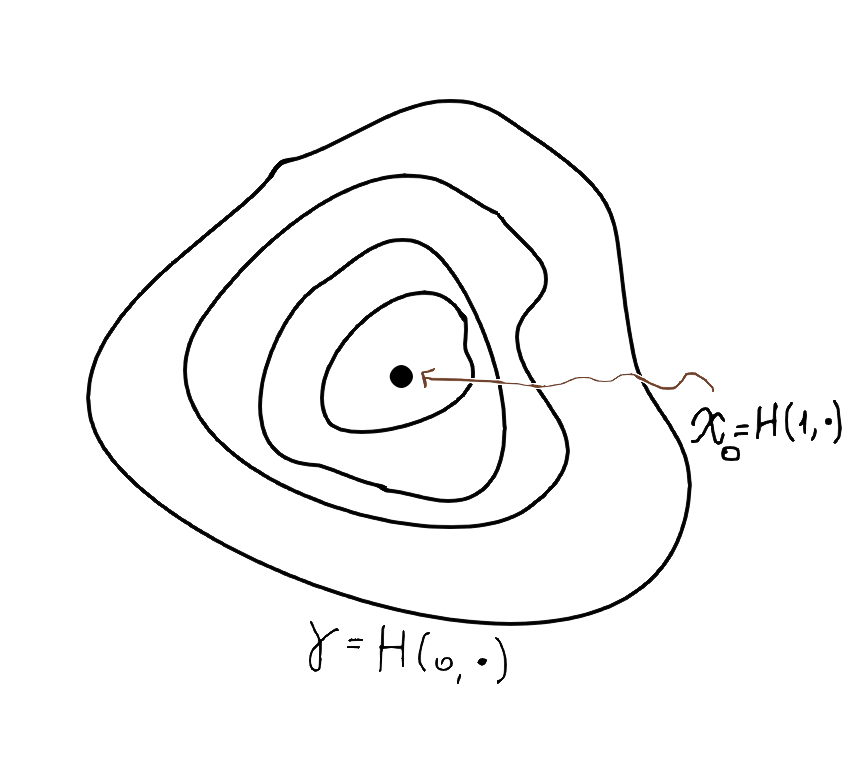
\includegraphics{immagini/omotopia.png}
	\caption{Rappresentazione di un'omotopia: la curva $\gamma$ viene strizzata fino a diventare il punto $x_0$.}
\end{figure}
\begin{definition}[insieme semplicemente connesso]
	Diremo che $E \subseteq \mathbb{R}^n$ è un insieme semplicemente connesso se
	\begin{enumerate}[label=\protect\circled{\arabic*}]
		\item è connesso per archi;
		\item $\forall \gamma \in C^0([a, b], E)$ chiusa ha un punto $x_0 \in E$ a cui è omotopa in $E$.
	\end{enumerate}
\end{definition}
\begin{remark}
	Un esempio di insieme semplicemente connesso è $\Omega = \mathbb{R}^2 \setminus \{(x, y) \in \mathbb{R}^2 : y = 0, x > 0 \}$: questo perché è possibile deformare con continuità la curva chiusa $\gamma$ affinché scavalchi la parte dell'insieme esclusa. Un insieme non semplicemente connesso è $\mathbb{R}^2 \setminus \{ (0, 0) \}$ 
	siccome prendendo una curva sufficientemente vicina all'origine, per esempio, e un raggio sufficientemente grande la curva sarebbe costretta a passare per l'origine che è però esclusa.
	Per $n > 2$ avremo che $\mathbb{R}^n \setminus \{ (0, 0) \}$ è semplicemente connesso siccome è possibile deformare la curva, sfruttando le dimensioni "in più" rispetto ad $\mathbb{R}^2$, per scavalcare l'origine.
\end{remark}
\begin{remark}
	Sia $\Omega = \mathbb{R} \setminus S$ e $S = q + \mathbb{R}v$. $S=\{q+tv : t \in \mathbb{R} \}, q, v \in \mathbb{R}^3$, ovvero lo spazio tridimensionale senza una realtà. Allora $\Omega$ non è semplicemente connesso, siccome prendendo una circonferenza sufficientemente vicina alla retta e con un raggio maggiore della distanza dal punto alla retta, la curva sarebbe costretta a "toccare" la retta per poter essere omotopa ad un punto, pertanto
	non è un insieme semplicemente connesso.
\end{remark}
\begin{prop}[gli insiemi convessi sono semplicemente connessi]
	Sia $E \subseteq \mathbb{R}^n$, allora $E$ è semplicemente connesso
\end{prop}
\begin{proof}
	Se $E$ è convesso e $\gamma: [a, b] \to E$ è chiusa e continua scelgo $x_0 \in E$ e osservo che, preso
	\begin{align*}
	&H(s,t) = sx_0 + \gamma(t) (1 - s) & &0 \leq s \leq 1,
	\end{align*}
	per la convessità di $E$ avremo che $H(s, t) \in E$. Avremo per $s = 0$ che $H(0, t)=\gamma(t)$ e per $s=1$ che $H(1, t)=x_0$. Siccome $H$ è continua, avremo che $H$ è un'omotopia in $E$ tra $\gamma$ e $x_0$.
\end{proof}
\begin{theorem}
	Sia $\Omega \subseteq \mathbb{R}^n$ aperto e semplicemente connesso e sia $\omega \in C^1(\Omega, (\mathbb{R}^n)^*)$. Allora
	\begin{align*}
		\omega \text{ è chiusa } \iff \omega \text{ è esatta }. 
	\end{align*}
	Equivalentemente, se $F \in C^1(\Omega, \mathbb{R}^n)$ allora
	\begin{align*}
		F \text{ è irrotazionale } \iff F \text{ è conservativo }.
	\end{align*}
\end{theorem}
\begin{proof} la dimostrazione verrà fatta, senza perdere di generalità, nel caso delle $1-$forme differenziali. \\
	$\boxed{\Leftarrow}:$ già dimostrato nella proposizione~\ref{prop:esattezza_imp_chiusura} \\
	$\boxed{\Rightarrow}:$ %questa dimostrazione si rifà a delle proprietà del \emph{prodotto wedge}, che trovate nelle appendici.
	%Sappiamo che $\omega = a_1(x)dx_1 + \ldots + a_n(x)dx_n$ e, siccome la forma $\omega$ è chiusa, abbiamo che $d\omega = 0$, dunque
	%$$
	%d\omega = d(a_1(x)dx_1 + \ldots a_n(x)dx_n) = \sum_{i=1}^n da_i \wedge dx_i = \sum_{i=1}^n \left( \sum_{j=1}^n \frac{\partial a_i}{\partial x_j} dx_j \right) \wedge dx_i \stackrel{\text{linearità del prodotto wedge}}{=} \sum_{i=1}^n \sum_{j=1}^n \frac{\partial a_i}{\partial x_j} dx_j \wedge dx_i
	%$$
	fissiamo $x_0 \in \Omega$ e, preso $x \in \Omega$, consideriamo la funzione
	$$
		F(x) = \int_\gamma \omega
	$$
	dove $\gamma(t) : [0, 1] \mapsto \Omega$ è una curva con $\gamma(t)=(1-t) x_0 + tx$. Per definizione di integrale curvilineo di seconda specie avremo che
	$$
		\int_0^1 \omega(\gamma(t)) \dot{\gamma}(t) dt = \int_0^1 \omega((1-t)x_0 + tx)(x-x_0)dt
	$$
	ma possiamo derivare sotto il segno di integrale (la derivata di $\omega \circ \gamma$ esiste ed è continua siccome composizione di funzioni derivabili lungo una direzione $x_j$):
	$$
	\partial_{x_j} F(x) = \int_0^1 \partial_{x_j} \left(\sum_{i=1}^n a_i((1-t)x_0 + tx)(x_i-x_{0_i}) \right) = \int_0^1 \left(a_j((1-t)x_0 + tx) + \sum_{i=1}^n t\frac{\partial a_i}{\partial x_j}((1-t)x_0 + tx)(x_i - x_{0_i}) \right)dt
	$$
	adesso osserviamo che la chiusura della $1-$forma differenziale implica che $\forall 1 \leq i < j \leq n$
	$$
	\frac{\partial a_i}{\partial x_j} = \frac{\partial a_j}{\partial x_i}.
	$$
	Inoltre osserviamo che, tramite il teorema del differenziale della composizione, abbiamo che 
	$$
		\frac{\partial}{\partial t} a_j((1-t)x_0 + tx) = Da_j((1-t)x_0 + tx) \, D((1-t)x_0 + tx)(t) = \sum_{i=1}^n \frac{\partial a_j}{\partial x_i}(x_i - x_{0_i})
	$$
	dunque, effettuando questa sostituzione nell'integrale di sopra, otterremo che
	\begin{align*}
	&\partial_{x_j} F(x) = \int_0^1 \partial_{x_j} \left(a_j((1-t)x_0 + tx) + \sum_{i=1}^n t\frac{\partial a_j}{\partial x_i} \left( ((1-t)x_0 + tx) (x_i - x_{0_i}) \right) \right) dt = \\
	&=\int_0^1 \left( a_j((1-t)x_0 + tx) + t\frac{\partial}{\partial t} \left[ a_j((1-t)x_0 + tx) \right] \right)dt = \int_0^1 \frac{\partial}{\partial t} \left( ta_j((1-t)x_0 + tx) \right)dt = a_j(x) 
	\end{align*}
	dunque $dF=\omega$, il che conclude la dimostrazione.
\end{proof}
\section{Campi vettoriali radiali}
\begin{definition}[campo vettoriale radiale]
	Consideriamo $h: (0, +\infty) \mapsto \mathbb{R}$ continua e $F: \mathbb{R}^n \setminus \{\underline{0} \} \to \mathbb{R}^n$ con $F(x) = h(|x|)x$.
	Diremo allora che $F$ è un campo vettoriale radiale.
\end{definition}
\begin{remark}
Siccome $\nabla |x| = \frac{x}{|x|} \, \forall x \neq \underline{0}$ allora $F(x) = |x|h(|x|)\frac{x}{|x|} \implies F(x) = |x| \, h(|x|)\nabla |x|$
\end{remark}
\begin{prop}[i campi radiali sono conservativi]
	Sia $F$ un campo vettoriale radiale, allora $F$ è conservativo
\end{prop}
\begin{proof}
	Possiamo pensare di definire
	$$
	U(s) = \int_1^s t h(t)dt \text{ con } s > 0 
	$$
	e posto $V(x) = U(|x|) \implies$
	$$
	\implies \nabla V(x) = \sum_{j=1}^n \frac{\partial}{\partial x_j} U(|x|)e_j
	$$
	ma osserviamo che $\frac{\partial U(|x|)}{\partial x_j} = \frac{\partial U(|x|)}{\partial |x|} \frac{\partial |x|}{\partial x_j} = U'(|x|) \frac{x_j}{|x|}$ dove osserviamo che $\frac{\partial |x|}{\partial x_j} = \frac{1}{\cancel{2}} \frac{\cancel{2}x_j}{\sqrt{\sum\limits_{i=1}^n x_i^2}}$
	$$
		\sum_{j=1}^n U'(|x|) \frac{x_j}{|x|}e_j = \frac{U'(|x|)}{|x|} \sum_{j=1}^n x_j e_j = \frac{U'(|x|)}{|x|} |x| = U'(|x|) = |x| \, h(|x|)
	$$
	dove si è usato il teorema fondamentale del calcolo per calcolare la derivata di $U(|x|)$ rispetto a $|x|$ siccome $\frac{\partial}{\partial |x|} = \frac{\partial}{\partial |x|} \int_1^{|x|} t h(t) dt = th(t)|_{t=|x|} = |x|h(|x|)$
\end{proof}
\begin{remark}
	Osserviamo che per $n=2$ il nostro campo vettoriale è definito su $\mathbb{R}^2 \setminus \{ (0, 0) \}$, che ricordiamo essere un insieme non semplicemente connesso. Detto questo, non è detto che non vi siano delle forme differenziali esatte: un esempio
	è il campo gravitazionale che è un campo conservativo.
\end{remark}
Similmente, possiamo definire le $1-$forme differenziali radiali nella seguente maniera
\begin{definition}[$1-$forma differenziale radiale]
	Sia $h(x) \in C^0((0, +\infty), \mathbb{R})$ e sia $\omega \in C^{\infty}(\mathbb{R}^n \setminus \{ \underline{0} \}, (\mathbb{R}^n)^*)$ è una $1-$ forma differenziale radiali se
	$$
		\omega(x) = h(|x|)\sum_{j=1}^n x_j dx_j
	$$
\end{definition}
Come prima, avremo che è esatta con primitiva $P(x)=U(|x|)$, dove $U(s) = \int_1^s th(t)dt$ e $dP(x)=\omega(x)$.
	\chapter{Cenni alla misura di Lebesgue}

In questo capitolo affronteremo il concetto di misura e daremo alcuni accenni all'impostazione teorica data da Lebesgue nello sviluppo
del suo concetto di misura. Alcuni approfondimenti inseriti sono stati presi da \cite{rudin}, tuttavia per una trattazione più accurata e completa rimando a \cite{measure_theory}.

\section{La misura esterna}
Vogliamo adesso determinare una funzione di insiemi $m_n: \mathcal{P}(\mathbb{R}^n) \to [0; +\infty]$ che rappresenta il nostro concetto intuitivo di \emph{volume} dell'insieme, detto \emph{misura dell'insieme}. \\
L'intuizione ci porta a pensare che questa funzione goda delle seguenti proprietà:
\begin{enumerate}[label=\protect\circled{\arabic*}]
	\item $m_n(\emptyset) = 0$
	\item Se $A, B \subseteq X$ tali che $A \subseteq B \implies m_n(A) \leq m_n(B)$
	\item Se $A, B \subseteq X$ tali che $A \cap B = \emptyset \implies m_n(A \cup B) = m_n(A) + m_n(B)$
\end{enumerate}
\begin{definition}[misura di un intervallo e di un $n-$intervallo]
	Per ogni intervallo $I \subseteq \mathbb{R}$ limitato definiamo
	$$
	\mathit{l}(I) = \sup{I} - \inf{I}.
	$$
	Sia adesso $I_1 \times \ldots \times I_n \subseteq \mathbb{R}^n$ definiamo
	$$
		v_n \left( \varprod_{i=1}^n I_i \right) = \prod_{i=1}^n \mathit{l}(I_i) 
	$$
\end{definition}
\begin{definition}[misura di Lebesgue di un insieme $E$]
	Sia $E \subseteq \mathbb{R}^n$, definiamo la misura di Lebesgue di $E$ come
	\begin{equation}
		m_n(E) = \inf \left\{ \sum_{i=1}^{+\infty} v_n(J_i) : E \subseteq \bigcup_{i=1}^{+\infty} J_i \text{ e } J_i \subseteq \mathbb{R}^n \text{ è un } n\text{-intervallo} \right\}
		\label{eq:def_lebesgue}
	\end{equation}
\end{definition}
\begin{remark}
	Con un procedimento abbastanza simile a come abbiamo fatto per la misura di Peano-Jordan, approssimiamo un insieme $E$ tramite degli $n-$intervalli dall'esterno. La sostanziale differenza, per come stiamo introducendo la misura di Lebesgue, è che stiamo approssimando solamente "da fuori".
	In questa maniera possiamo misurare una classe di insiemi più ampia rispetto a quella della misura di Peano-Jordan, in cui si richiedeva che la misura approssimata "da dentro" coincideva con la misura approssimata "da fuori".
\end{remark}
Come vedremo fra un po', esistono degli insiemi che non sono misurabili per Lebesgue; dunque per ogni sottoinsieme di $X$ non è possibile definire una misura $m_n$ (non su tutti gli insiemi essa è additiva come richiesto, dunque non è una misura). \\ Ci basta, tuttavia, definire una misura \emph{esterna}, ovvero
una funzione che stima il volume di un qualunque insieme $E$ attraverso una collezione di insiemi che ricopre dall'esterno il nostro insieme. In questa maniera è possibile definire una funzione d'insieme definita per ogni insieme, tuttavia non rispetta la proprietà di additività numerabile che noi vogliamo per effettuare operazioni come i limiti: tramite 
il teorema di Caratheodory si può tuttavia mostrare che, presa una misura esterna $\mu^*$, esiste uno spazio di misura in cui la misura coincide con quella esterna. \\
Successivamente, dovremo cercare un criterio con cui stabilire se un insieme $E$ è misurabile o meno.
\begin{definition}
	Diremo che $\mu^*: \mathcal{P}(X) \mapsto [0; +\infty]$ è una misura esterna se
	\begin{enumerate}[label=\protect\circled{\arabic*}]
		\item $\mu^*(\emptyset) = 0$;
		\item $\mu^*(E) \leq \sum\limits_{i=1}^{+\infty} \mu^*(E_i)$ se $E \subseteq \bigcup\limits_{i=1}^{+\infty} E_i$
	\end{enumerate}
\end{definition}
\begin{prop}[monotonia della misura esterna]
	Se $\mu^*$ è una misura esterna allora
	$$
	A \subseteq B \implies \mu^*(A) \leq \mu^*(B)
	$$
	\label{prop:monotonia}
\end{prop}
\begin{proof}
	Consideriamo $E = A$ e il seguente insieme
	\begin{align*}
	E_j = \begin{cases} B & j=1 \\ \emptyset & j \geq 2	\end{cases}
	\end{align*}
	osserviamo allora che $E \subseteq \bigcup\limits_{i=1}^{+\infty} E_i$ allora
	$$
	\mu^*(E) = \mu^*(A) \stackrel{\text{per la \circled{2}}}{\leq} \sum_{j=1}^{+\infty} \mu^*(E_j) = \mu^*(E_1) = \mu^*(B)
	$$
	ovvero
	$$
	\mu^*(A) \leq \mu^*(B)
	$$
\end{proof}
\begin{prop}[subadditività finita]
	Le misure esterne sono finitamente subadditive, ovvero preso $E_1, \ldots, E_k$ avremo che 
	$$
	\mu^* \left( \bigcup_{i=1}^{k} E_i \right) \leq \sum_{i=1}^k \mu^*(E_i)
	$$
	\label{prop:sub_finita}
\end{prop}
\begin{proof}
	Siano $E_1, \ldots, E_k \subseteq \mathbb{R}^n$. Imponendo che $\forall j > k, E_j = \emptyset$, allora
	$$
	\forall E \subseteq \bigcup_{i=1}^{+\infty} E_i, \mu^*(E) \leq \sum_{i=1}^{+\infty} \mu^*(E_i) = \sum\limits_{i=1}^{k} \mu^*(E_i) + \sum\limits_{i=k+1}^{+\infty} \mu^*(\emptyset) = \sum\limits_{i=1}^k \mu^*(E_i) \implies \mu^*(E) \leq \sum_{i=1}^k \mu^*(E_i)
	$$
	ma allora, siccome abbiamo banalmente che $\bigcup\limits_{i=1}^{k} E_i \subseteq \bigcup\limits_{i=1}^k E_i$, allora
	$$
	\mu^* \left( \bigcup_{i=1}^k E_i \right) \leq \sum_{i=1}^k \mu^*(E_i)
	$$
\end{proof}
Vogliamo adesso mostrare che la funzione d'insieme $m_n$ da noi definita è effettivamente una misura esterna, dunque è un buon punto di partenza per poter definire una misura che possieda le proprietà che abbiamo enunciato all'inizio di questo capitolo, siccome il teorema di 
Caratheodory ci assicura di poter trovare uno spazio di misura in cui la misura esterna $\mu^*$ è effettivamente una misura (ovvero è additiva su ogni insieme dello sapzio e non subadditiva).
\begin{prop}[misura di Lebesgue è una misura esterna]
	$m_n: \mathcal{P}(X) \to [0; +\infty]$ è una misura esterna
	\label{prop:lebesgue_mis_esterna}
\end{prop}
\begin{proof}
	La dimostrazione consiste nel mostrare che $m_n: \mathcal{P}(X) \mapsto [0; +\infty]$ gode delle proprietà della misura esterna. \\
	La \circled{1} segue banalmente, siccome l'$n-$intervallo nullo è un ricoprimento dell'insieme nullo, dunque $m_n(\emptyset) = 0$.
	Per la \circled{2}, supponiamo naturalmente che $\sum\limits_{i=1}^{+\infty} m_n(E_i) < +\infty$ (altrimenti è banale) e prendiamo un insieme $E \subseteq \bigcup\limits_{i=1}^{+\infty} E_i$, osservando che $\forall i \in \mathbb{N}, E_i \subseteq \bigcup\limits_{k=1}^{+\infty} I_{k}^{(i)}$, pertanto
	$$
		E \subseteq \bigcup_{i=1}^{+\infty} \bigcup_{k=1}^{+\infty} I_k^{(i)}
	$$
	e questo vale per ogni ricoprimento di $\bigcup\limits_{i=1}^{+\infty} E_i$, dunque anche per quello che "fornisce" la misura di $\bigcup\limits_{i=1}^{+\infty} E_i$
	$$
		m_n(E) \leq \inf \left\{\sum_{i=1} l(E_i) \right\} = m_n \left( \bigcup_{i=1}^{+\infty} E_i \right)
	$$
	resta da mostrare che $m_n( \bigcup\limits_{i=1}^{+\infty} E_i ) \leq \sum\limits_{i=1}^{+\infty} m_n(E_i)$ . Questo può essere fatto fissando $\varepsilon > 0$ e osservando che $\forall i \in \mathbb{N}, \exists \bigcup\limits_{k=1}^{+\infty} I_{i}^{(k)} \supseteq E_i : \sum\limits_{k=1}^{+\infty} l(I_i^{(k)}) < m_n(E_i) + \frac{\varepsilon}{2^{i+1}}$, dunque
	$$
	m_n \left( \bigcup_{i=1}^{+\infty} E_i \right) \leq \sum_{i=1}^{+\infty} \sum_{k=1}^{+\infty} l(I_{i}^{(k)}) < \sum_{i=1}^{+\infty} (m_n(E_i) + \frac{\varepsilon}{2^{i+1}}) = \varepsilon + \sum_{i=1}^{+\infty} m_n(E_i)
	$$
	e, siccome $\varepsilon$ era arbitrario, otteniamo la tesi facendo il limite.
\end{proof}
\begin{definition}[insieme misurabile secondo Lebesgue]
	Diremo che $A \subseteq X$ è misurabile secondo Lebesgue se
	$$
	\forall S \subseteq X \implies m_n(S) = m_n(A \cap S) + m_n(S \setminus A)
	$$
	\label{def:mis_lebesgue}
\end{definition}
Per ogni insieme $X$ definiamo con $\mathfrak{M}(X)$ la classe di tutti gli insiemi misurabili secondo Lebesgue.
\begin{definition}[$\sigma-$algebra]
	Diremo che $\mathcal{F} \subseteq \mathcal{P}(X)$ è una $\sigma-$algebra se valgono
	\begin{enumerate}[label=\protect\circled{\arabic*}]
		\item $\emptyset, X \in \mathcal{F}$;
		\item $A \in \mathcal{F} \implies (X \setminus A) \in \mathcal{F}$
		\item $\{ A_j : j \geq 1 \} \subseteq \mathcal{F} \implies \bigcup\limits_{i=1}^{+\infty} A_i \in \mathcal{F}$
	\end{enumerate}
\end{definition}
\begin{definition}[misura]
	Diremo che $\mu: \mathcal{F} \mapsto [0; +\infty]$ è una misura se
	\begin{enumerate}[label=\protect\circled{\arabic*}]
		\item $\mathcal{F}$ è una $\sigma-$algebra;
		\item $\mu(\emptyset) = 0$;
		\item Se $( \{A_i : i \geq 1 \} \subseteq \mathcal{F}) \wedge (\forall i \neq j, A_i \cap A_j = \emptyset$) allora
		$$
			\mu \left( \bigcup_{i=1}^{+\infty} A_i \right) = \sum_{i=1}^{+\infty} \mu(A_i)
		$$
	\end{enumerate}
\end{definition}
\begin{theorem}
	La classe dei misurabili $\mathfrak{M}(X)$ è una $\sigma-$algebra e $m_n:\mathfrak{M}(X) \to [0; +\infty]$ è una misura
\end{theorem}
Diremo allora che $m_n: \mathfrak{M}(X) \to [0; +\infty]$ è la misura di Lebesgue su $X$. Per lo più noi lavoreremo supponendo che $X=\mathbb{R}^n$.
\begin{prop}
	La misura $m_n: \mathfrak{M}(X) \to [0; +\infty]$ è finitamente additiva
\end{prop}
\begin{proof}
La dimostrazione è equivalente a quella della proposizione~\ref{prop:sub_finita} sostituendo opportunamente alle minorazione le eguaglianze.
\end{proof}
\begin{remark}
Ammettendo l'assioma della scelta è possibile mostrare che esistono degli insiemi che non sono misurabili (come ampiamente detto in precedenza). L'esempio più famoso è
l'insieme di Vitali, che si può costruire dentro un qualunque insieme di misura positiva $E \in \mathfrak{M}(\mathbb{R}^n)$. Dalla definizione di misurabilità allora $\exists S_0 \subseteq \mathbb{R}^n$
tale che 
$$
m_n(S_0) \leq m_n(S_0 \cap E) + m_n(S_0 \setminus E)
$$
dunqque si perderebbe la $\sigma-$additività su insiemi disgiunti.
\end{remark}
\subsection{Insiemi trascurabili}
\begin{definition}[insiemi trascurabili]
	Diremo che $Z \subseteq \mathbb{R}^n$ ha misura nulla oppure che è trascurabile se $m_n(Z) = 0$
\end{definition}
\begin{exercise}
	Mostrare che un punto $x \in \mathbb{R}^n$ ha misura nulla
\end{exercise}
\begin{proof}[Svolgimento]
	Sia $x \in \mathbb{R}^n$ e consideriamo un $n-$intervallo $\varprod\limits_{i=1}^n I_i$ dove $I_i = (x_i - \frac{\varepsilon}{2}, x_i + \frac{\varepsilon}{2})$ ($x_i$ rappresenta la $i-$esima componente del punto $x$), dunque rappresenta un cubo di \emph{volume} pari a $\varepsilon^n$ per $i \in \{1, \ldots, n \}$ con $\varepsilon > 0$. Allora possiamo osservare che
	$$
	\{ x \} \subseteq \bigcup_{i=1}^{+\infty} J_i
	$$
	dove
	\begin{align*}
		J_i = \begin{cases}
			\varprod\limits_{i=1}^n (x_i - \frac{\varepsilon}{2}, x_i + \frac{\varepsilon}{2}) \\
			\emptyset
		\end{cases}
	\end{align*}
	ma allora
	$$
	m_n(\{ x \}) \subseteq \bigcup_{i=1}^{+\infty} v_n(J_i) = \varepsilon^n
	$$
	ma allora, siccome $\varepsilon > 0$ è un valore arbitrario, possiamo farne il limite per $\varepsilon \to 0$, dunque $m_n(\{ x \}) = 0$.
\end{proof}
\begin{prop}
	Se $Z \subseteq \mathbb{R}^n$ è numerabile, allora
	$$
		m_n(Z) = 0
	$$
\end{prop}
\begin{remark}
	Non tutti gli insiemi a misura nulla sono numerabili: un esempio è l'insieme di Cantor.
\end{remark}
\begin{proof}
	Se $Z$ è numerabile allora
	$$
		Z = \bigcup_{i=1}^{+\infty} \{ x_i \}
	$$
	dove $x_i: \mathbb{N} \to Z$ dunque
	$$
	m_n(Z) \leq \sum_{i=1}^{+\infty} m_n(\{ x_i \}) = 0 \implies m_n(Z) = 0
	$$
\end{proof}
\begin{cor}
	$\mathbb{Q}^n$ è un insieme trascurabile
\end{cor}
\begin{proof}
$\mathbb{Q}^n \cong \mathbb{N}$ dunque $m_n(\mathbb{Q}^n) = 0$
\end{proof}
\begin{cor}
	Gli insiemi a misura nulla sono misurabili per Lebesgue.
	\label{cor:mis_nulla_misur}
\end{cor}
\begin{proof}
In virtù della definizione~\ref{def:mis_lebesgue} dobbiamo verificare che, preso $Z$ insieme trascurabile, allora
$$
\forall S \subseteq \mathbb{R}^n, m_n(S) = m_n(S \setminus Z) + m_n(S \cap Z)
$$
Ora osserviamo che, siccome $S = (S \setminus Z) \cup (S \cap Z)$, avremo per la subadditività finita (di cui gode $m_n$ siccome nella proposizione~\ref{prop:lebesgue_mis_esterna} abbiamo mostrare che è una misura esterna)
che
$$
m_n(S) \leq m_n(S \setminus Z) \cup (S \cap Z)
$$
Per la disuguaglianza opposta osserviamo che
\begin{align*}
m_n(S) \geq m_n(S \setminus Z) \text{ e } m_n(Z) \geq m_n(S \cap Z)
\end{align*}
per monotonia della misura esterna (proposizione~\ref{prop:monotonia}), ma siccome $0=m_n(Z) \geq m_n(S \cap Z) \implies m_n(S \cap Z) = 0$ allora
$$
m_n(S) \geq m_n(S \setminus Z) = m_n(S \setminus Z) + m_n(S \cap Z) \implies m_n(S) \geq m_n(S \setminus Z) + m_n(S \cap Z)
$$
dunque $m_n(S) = m_n(S \setminus Z) + m_n(S \cap Z)$, ovvero la tesi.
\end{proof}
\begin{theorem}[gli aperti sono misurabili]
	Tutti gli aperti di $\mathbb{R}^n$ sono misurabili secondo Lebesgue
\end{theorem}
Per dimostrare questo teorema abbiamo bisogno del seguente lemma:
\begin{lemma}
Ogni aperto di $\mathbb{R}^n$ è unione numerabile di $n-$intervalli a due a due disgiunti
\end{lemma}
\begin{proof}
	Sia $A \subseteq \mathbb{R}^n$ aperto non vuoto. Allora possiamo considerare la famiglia degli $n-$intervalli $I \subseteq A$ ad estremi razionali, ovvero:
	$$\mathcal{V} = \{I = \prod_{i=1}^n (a_i, b_i] : I \subseteq A, a_i, b_i \in \mathbb{Q} \, \, \forall i \in \{1, \ldots, n\} \}$$
	Siccome ogni $n-$intervallo all'interno di $\mathcal{V}$ può essere messo in corrispondenza biunivoca con la $2n-$upla $(a_1, \ldots, a_n, b_1, \ldots, b_n) \in \mathbb{Q}^{2n}$ che è un insieme numerabile, allora anche $\mathcal{V}$ è un insieme numerabile. E' banale l'inclusione $\bigcup\limits_{I \in A} I \subseteq A$ (per definizione di $\mathcal{V}$), vogliamo
	adesso mostrare che vale anche l'inclusione opposta: sia $x \in A$ e, siccome $A$ è aperto, avremo che 
	$$\forall y \in A, \exists \varepsilon > 0 : \{y = (y_1, \ldots, y_n) \in \mathbb{R}^n : |y_i - x_i| < \varepsilon \, \, \forall i \in \{1, \ldots, n \} \} \subseteq A$$
	Siccome $\mathbb{Q}$ è denso in $\mathbb{R}$ avremo che $\forall i \in \{1, \ldots, n \}, \exists \alpha_i, \beta_i \in \mathbb{Q}$ tali che
	$$
	x_i - \varepsilon < \alpha_i < x_i < \beta_i < x_i + \varepsilon 
	$$
	Dunque avremo che l'$n-$intervallo $I'=\prod\limits_{i=1} (\alpha_i, \beta_i]$ contiene il punto $x$, dunque $x \in \mathcal{V} \implies x \in \bigcup\limits_{I \in \mathcal{V}} I \implies A \subseteq \bigcup_{I \in \mathcal{V}} I$. Concludiamo
	che $A = \bigcup\limits_{i=1} I$. \\
	Mostriamo adesso che possiamo prendere gli $n-$intervalli a due a due disgiunti. Consideriamo $A = \bigcup_{i=i}^{+\infty} I_i$ ma allora, posto $J_i = I_i \setminus \bigcup_{j=1}^{i-1} I_j$, possiamo vedere facilmente che
	$$
	\bigcup_{i=1}^{+\infty} I_i = \bigcup_{i=1}^{+\infty} J_i = A
	$$
\end{proof}
Siamo pronti adesso a dimostrare il teorema:
\begin{proof}[Dimostrazione (del teorema)]
	Sia $A$ un insieme aperto. Per il lemma precedente sappiamo che $A = P = \bigcup_{k=1}^{+\infty} I_i$ dove $I_i$ è un $n-$intervallo, dunque $m_n(P \setminus A) = m_n(\emptyset) = 0$.
	Pertanto $P \setminus A \in \mathfrak{M}(\mathbb{R}^n)$ e $P \in \mathfrak{M}(\mathbb{R}^n)$ siccome unione di $n-$intervalli. 
\end{proof}
\begin{cor}
	Tutti gli insiemi chiusi di $\mathbb{R}^n$ sono misurabili secondo Lebesgue
\end{cor}
\begin{proof}[Dimostrazione (del corollario)]
	Siccome $m_n: \mathfrak{M}(\mathbb{R}^n) \to [0; +\infty]$ allora $\mathfrak{M}(\mathbb{R}^n)$ è una $\sigma-$algebra, dunque se $A \in \mathfrak{M}(\mathbb{R}^n) \implies A^c \in \mathfrak{M}(\mathbb{R}^n)$.
\end{proof}
\begin{cor}
	Tutte le unioni e le intersezioni numerabili di insiemi chiusi o aperti sono ancora misurabili secondo Lebesgue
\end{cor}
\begin{proof}
	Se $\{ B_i : i \geq 1 \} \subseteq \mathfrak{M}(\mathbb{R}^n) \implies \bigcup\limits_{i=1}^{+\infty} B_i \in \mathfrak{M}(\mathbb{R}^n)$ perché $\mathfrak{M}(\mathbb{R}^n)$ è una $\sigma-$algebra, mentre per le intersezioni numerabili abbiamo che se $B_i \in \mathfrak{M}(\mathbb{R}^n) \implies B_i^c \in \mathfrak{M}(\mathbb{R}^n)$ (sempre per le proprietà delle $\sigma-$algebre)
	e, per le leggi di De Morgan, avremo che $\left(\bigcup\limits_{i=1}^{+\infty} B_i^c \right)^c = \bigcap\limits_{i=1}^{+\infty} B_i \in \mathfrak{M}(\mathbb{R}^n)$
\end{proof}
\section{Funzioni misurabili secondo Lebesgue}
Andiamo adesso ad affrontare il concetto di funzione misurabile, il quale ci condurrà, naturalmente, verso il concetto di integrale di Lebesgue
\begin{definition}[funzioni misurabili secondo Lebesgue]
Sia $E \in \mathfrak{M}(\mathbb{R}^n)$ misurabile e $f: E \to \bar{\mathbb{R}}$. Diremo che $f$ è misurabile secondo Lebesgue se $\forall t \in \mathbb{R}$ l'insieme $f^{-1}([-\infty, t)) \in \mathfrak{M}(\mathbb{R}^n)$, ovvero esso è misurabile.
\end{definition}
\begin{remark}(\textbf{Topologia di $[-\infty, \infty]$})
	Ogni aperto di $[-\infty, +\infty]$ è un'unione arbitraria di intervalli che possono essere sia aperti oppure del tipo $[-\infty, t)$ o $(t, +\infty]$.
\end{remark}
\begin{prop}[caratterizzazione delle funzioni misurabili]
	$E \in \mathfrak{M}(\mathbb{R}^n), f: E \to \bar{\mathbb{R}}$ è misurabile se e solo se $\forall O \subseteq \bar{\mathbb{R}}$ aperto di $[-\infty, +\infty]$ abbiamo che $f^{-1}(O) \in M(\mathbb{R}^n)$
\end{prop}
\begin{prop}[le funzioni continue sono misurabili]
	Se $E \in \mathcal{R}^n, f: E \to \mathbb{R}$ è continua, allora è misurabile
\end{prop}
\begin{proof}
	Se $O \subseteq [-\infty, +\infty]$ è un aperto contenuto in $\mathbb{R}$ in realtà è un aperto di $\mathbb{R} \implies f^{-1}(O)$ è aperto in $E$ in virtù del teorema~\ref{thm:teo_cf1}, dunque avremo che $\exists \Omega \subseteq \mathbb{R}^n$ tale che
	$$
	f^{-1}(0) = E \cap \Omega \in \mathfrak{M}(\mathbb{R}^n) \implies f \text{ è misurabile }
	$$
	ovvero la tesi.
\end{proof}
\begin{prop}
	Se $f_n: E \to \bar{\mathbb{R}}$ è una successioni di funzioni misurabili e $f:E \to \bar{\mathbb{R}}$. Se $f_n \stackrel{n \to +\infty}{\to} f \, \, \forall x \in E$ allora $f$ è misurabile
\end{prop}
Prendiamo in causa una funzione che causava molti problemi all'integrale di Riemann, ovvero la funzione di Dirichlet. Al momento, consideriamo una sua \emph{variante} $\chi_k: [0, 1] \to \mathbb{R}$ definita come
\begin{align*}
	\chi_k(x) = \begin{cases}
		1 & \text{ se } x \in \{q_0, \ldots, q_k \} \\
		0 & \text{ se } x \not\in \{q_0, \ldots, q_k \}
	\end{cases}
\end{align*}
allora $\chi_k \stackrel{n \to +\infty}{\to} \chi$, ovvero la funzione di Dirichlet. Grazie alla precedente proposizione siamo in grado di concludere che $\chi$ è misurabile per Lebesgue, ma non per Riemann (sebbene $\forall k, \chi_k$ è Riemann-integrabile).
\begin{exercise}
Mostrare la misurabilità di $\chi$ tramite la definizione di funzione misurabile secondo Lebesgue.
\end{exercise}
\begin{proof}[Svolgimento]
	Osserviamo che $\chi: [0, 1] \mapsto \{0, 1\}$. Mostriamo il seguente lemma
	\begin{lemma}
		Sia $f: A \mapsto B$ e presi $B_1, B_2 \subseteq B$ allora
		$$
			f^{-1}(B_1 \cup B_2) = f^{-1}(B_1) \cup f^{-1}(B_2)
		$$
	\end{lemma}
	\begin{proof}
		Mostriamo che $f^{-1}(B_1 \cup B_2) \subseteq f^{-1}(B_1) \cup f^{-1}(B_2)$: per definizione sappiamo che $f^{-1}(B_1 \cup B_2) = \{x \in A: f(x) \in B_1 \cup B_2 \} \implies f(x) \in B_1 \vee f(x) \in B_2 \implies x \in f^{-1}(B_1) \vee x \in f^{-1}(B_2)$.
		Mostriamo che $f^{-1}(B_1 \cup B_2) \supseteq f^{-1}(B_1) \cup f^{-1}(B_2)$: supponiamo, per assurdo, che $\exists x \in f^{-1}(B_1) \cup f^{-1}(B_2) : x \not\in f^{-1}(B_1 \cup B_2) \implies f(x) \in B_1 \vee f(x) \in B_2$ e $f(x) \not\in B_1 \cup B_2$, il che è un assurdo.
	\end{proof}
	Dunque, in virtù di questo lemma appena mostrato, avremo che
	$$
		\chi^{-1}(\{0, 1\}) = \chi^{-1}(\{0 \}) \cup \chi^{-1}(\{1 \})
	$$
\end{proof}
e abbiamo che $\chi^{-1}({0}) = \mathbb{Q} \cap [0, 1]$ che è un'unione numerabile di punti, ovvero i numeri razionali all'interno di questo intervallo che, in virtù del corollario~\ref{cor:mis_nulla_misur}, è misurabile. \\
L'intervallo restante, invece, sarebbe pari a $[0, 1] \setminus (\mathbb{Q} \cap [0,1])$ che, tuttavia, è misurabile siccome $[0,1]$ è misurabile, $\mathbb{Q} \cap [0,1]$ è misurabile e le differenze sono misurabili secondo Lebesgue per le proprietà delle $\sigma-$algebre.
\begin{prop}
	Se $f, g: E \to \bar{\mathbb{R}}$ sono misurabili, allora
	\begin{enumerate}[label=\protect\circled{\arabic*}]
		\item se $f+g$ è ben definita ovunque su $E$ allora $f+g$ è misurabile;
		\item se $\lambda \in \mathbb{R}$ e $\lambda f$ è ben definita ovunque, allora $\lambda f$ è misurabile;
		\item $E \mapsto \max\{f(x), g(x) \}$ e $E \mapsto \min\{f(x),g(x) \}$ sono misurabili;
		\item se $f_j: E \to \mathbb{R}$ è misurabile $\forall j \in \mathbb{N} \implies x \in E \to \sup\limits_{j \in \mathbb{N}} f_j(x)$ è misurabile.
	\end{enumerate}
	\label{prop:f_g_mis}
\end{prop}
\subsection{L'integrale di Lebesgue}
Per una buona costruzione della misura di Lebesgue, è comodo definire le operazioni algebriche in $[0; +\infty]$. Definiamo il prodotto come
\begin{equation*}
	xy = \begin{cases}
		xy & \text{se } \max\{x, y \} < +\infty \\
		+\infty & \text{se } \max\{x, y \} = +\infty \text{ e } \min\{x, y \} > 0 \\
		0 & \text{se } \max\{x, y \} = +\infty \text{ e } \min\{x, y \} = 0
	\end{cases}
\end{equation*}
Il terzo caso, che sembra patologico, si può facilmente interpretare in maniera geometrica: avendo in mente la teoria dell'integrazione, il prodotto fra $0 \cdot +\infty$ corrisponde a quella di un rettangolo illimitato con base di lunghezza infinita e
altezza nulla, dunque ha area "pari" a 0. \\
Introduciamo adesso la nozione di funzione semplice, concetto cardine per lo sviluppo dell'integrale di Lebesgue.
\begin{definition}[funzione semplice]
	$\varphi: E \to \mathbb{R}$ è una funzione semplice se $\varphi(E)=\{\lambda_1, \ldots, \lambda_k \} \subset \mathbb{R}$ dove $\lambda_i \neq \lambda_j \, \, \forall i \neq j \in \{1, \ldots, k \}$ dove
	$\varphi^{-1}(\lambda_i) = A_i \in \mathfrak{M}(\mathbb{R}^n) \, \, \forall i \in \{1, \ldots, k \}$.
\end{definition}
\begin{definition}[funzione caratteristica]
	$$
		\mathbb{1}_{A_i} = \begin{cases} 1 & x \in A_i \\ 0 & x \not\in A_i \end{cases}
	$$
\end{definition}
\begin{remark}
Segue banalmente che
$$
\varphi(x) = \sum_{i=1}^k \lambda_i \mathbb{1}_{A_i} (x)
$$
se $\varphi$ è una funzione semplice, naturalmente per opportuni $\lambda_1, \ldots, \lambda_k$ e $A_1, \ldots, A_k \in \mathfrak{M}(\mathbb{R}^n)$.
\end{remark}
Geometricamente non è difficile intuire che il volume sotto una funzione semplice (che assume valori pari a costanti che dipendono dalla regione di spazio) corrisponde ad un "solido" $n-$dimensionale con altezza $\lambda_j$ con $j \in \{1, \ldots, k \}$ e base pari alla "superficie" (naturalmente il termine usato qua è per rendere intuitiva la trattazione, ma non necessariamente è una superficie) 
del dominio. Nell'ipotesi di $\lambda_j \geq 0 \, \, \forall j \in \{1, \ldots, k \}$ (per non avere problemi con volumi negativi) allora possiamo già definire il concetto di integrale

\begin{definition}
	Sia $\varphi: E \to \mathbb{R}$ una funzione semplice con $\lambda_j \geq 0 \, \, \forall j \in \{1, \ldots, k \}$ definiamo il suo integrale come
	\begin{equation}
		I(\varphi) = \sum_{j=1}^n \lambda_j m_n(A_j)
		\label{def:int_funz_sempl}
	\end{equation}
\end{definition}
\begin{remark}
Si osservi che nella definzione~\ref{def:int_funz_sempl} compare il prodotto $0 \cdot +\infty$ quando $m_n(A_i) = +\infty$ e $\lambda_i = 0$.
\end{remark}
\begin{definition}[integrale di Lebesgue]
	Data $f: E \to [0; +\infty]$ misurabile allora
	$$
		\int_E f(x)dx = \sup\{I(\varphi) : 0 \leq \varphi \leq f \text{ e } \varphi \text{ è semplice } \}
	$$
\end{definition}
Introdurremo le seguenti notazioni per l'integrale di Lebesgue
$$
\int_E f(x)dx = \int_E f(x_1, \ldots, x_n)dx_1, \ldots dx_n = \int_E f = \int_E f(x)dm_n(x) = \int_E fdm_n 
$$
\begin{remark}
Segue subito dalla definizione che se $f, g: E \to [0; +\infty]$ sono misurabili e $f \leq g$ su $E$ allora
$$
\int_E f \leq \int_E g
$$
\end{remark}
\begin{remark}
Se $E \in \mathfrak{M}(\mathbb{R}^n) \implies \mathbb{1}_E$ è misurabile e vale
$$
m_n(E) = \int_{\mathbb{R}^n} \mathbb{1}_E dm_n
$$
\end{remark}
\begin{remark}
Se $\varphi: E \to [0; +\infty]$ è semplice allora $\int\limits_E \varphi dm_n = I(\varphi) = \sum\limits_{i=1}^k \lambda_i m_n(E_i) $
\end{remark}
\begin{prop}
Sia $f: E \to \bar{\mathbb{R}}$ misurabile, allora anche $|f|$ è misurabile
\end{prop}
\begin{proof}
$|f| = f^+ + f^-$ dove $f^{+} = \max\{f, 0 \}$ e $f^{-}=\max\{0, -f \}$. Sappiamo, dalla proposizione~\ref{prop:f_g_mis}, che $\max\{f,0 \}$ e $\max\{-f, 0\}$ sono misurabili (dove abbiamo preso $g(x) = 0$) e la somma di due funzioni misurabili è misurabile.
\end{proof}
\begin{definition}[integrabilità secondo Lebesgue]
	Diremo che $f$ è integrabile secondo Lebesgue se
	$$
	\int_E |f(x)|dx < +\infty
	$$
	e, in tal caso, segue che
	$$
	\int_E f(x)dx = \int_E f^{+}(x)dx - \int_E f^{-}(x)dx
	$$
\end{definition}
\begin{definition}[proprietà quasi ovunque]
	Diremo che una proprietà o un'affermazione $P(x)$, con $x \in A$, vale quasi ovunque su $A$ se l'insieme dei punti
	$$
		Z = \{x \in A: P(x) \text{ è falsa } \}
	$$
	ha misura nulla, ovvero $m_n(Z) = 0$
\end{definition}
\begin{prop}
	Se $f: E \to [0; +\infty]$ misurabile allora
	\begin{enumerate}[label=\protect\circled{\arabic*}]
		\item $\int_E fdm_n = 0 \implies f=0$ quasi ovunque su $E$;
		\item $\int_E fdm_n < +\infty \implies f<+\infty$ quasi ovunque su $E$ 
	\end{enumerate}
\end{prop}
\begin{remark}
	La tesi del punto $\circled{1}$ ci dice che $f$ è quasi ovunque nulla su $E$ o equivalentemente che l'insieme $Z \subseteq E$ dei punti in cui $f$ assume dei valori positivi ha misura nulla, dunque $m_n(Z) = 0$. \\
	La tesi del punto $\circled{2}$ è analoga
\end{remark}
\begin{theorem}
	Siano $f, g: E \to \bar{\mathbb{R}}$ integrabili, ovvero $\int_E |f| dm_n < +\infty$ e $\int_E |g|dm_n < + \infty$, allora
	\begin{enumerate}[label=\protect\circled{\arabic*}]
		\item $\lambda, \tau \in \mathbb{R} \implies \lambda f + \tau g \in \mathbb{R}$ è quasi ovunque ben definita e sommabile. Inoltre
		$\int_E (\lambda f + \tau g) dm_n = \lambda \int_E f dm_n + \tau \int_E g dm_n$
		\item $|\int_E f dm_n| \leq \int_E |f|dm_n$
		\item $f \leq q$ quasi ovunque su $E \implies \int_E f \leq \int_E g$ 
	\end{enumerate}
\end{theorem}
\begin{theorem}[integrale di Riemann $1-$dimensionale con l'integrale di Lebesgue]
	Siano $-\infty \leq a < b \leq +\infty, I \subseteq \mathbb{R}$ intervallo tale che $a = \inf{I}$ e $b=\sup{I}$ e sia $f: I \to \mathbb{R}$ assolutamente integrabile secondo Riemann in senso generalizzato su $I$, ovvero
	$$
	\int_a^b |f(t)|dt < +\infty
	$$
	allora $f: I \to \mathbb{R}$ è integrabile (e quindi misurabile) secondo Lebesgue e
	\begin{equation}
		\int_a^b f(t)dt = \int_I fdm_n
		\label{eq:eqv_leb_riem}
	\end{equation}
\end{theorem}
\begin{remark}
	Osserviamo che l'equazione~\ref{eq:eqv_leb_riem} è il primo procedimento operativo con cui calcolare l'integrale di Lebesgue
\end{remark}
\begin{remark}
	Il teorema include anche il caso particolare in cui $I=[a,b]$.
\end{remark}
\begin{remark}(Esistenza di funzioni integrabili secondo Riemann in senso generalizzato ma non secondo Lebesgue) \\
	La funzione $f(x) = \frac{\sin{x}}{x}$ è integrabile (ma non assolutamente!) secondo Riemann in senso generalizzato nell'intervallo $[1, +\infty]$ ma non per Lebesgue. \\
	Mostriamo che non è integrabile secondo Lebesgue mostrando che
	$$
	\int_1^{+\infty} \Big| \frac{\sin{x}}{x} \Big|dx = +\infty
	$$
	Osserviamo che possiamo "spaccare" il nostro integrale, per linearità rispetto agli ordini di integrazione, fra multipli interi di $\pi$:
	\begin{align*}
	&\int_1^{+\infty} \Big| \frac{\sin{x}}{x} \Big| = \int_1^{\pi} \frac{\sin{x}}{x} + \sum_{k=1}^{+\infty} \int_{k\pi}^{(k+1)\pi} \Big|\frac{\sin{x}}{x} \Big|dx \geq \sum_{k=1}^{+\infty} \int_{k\pi}^{(k+1)\pi} \Big|\frac{\sin{x}}{(k+1)\pi} \Big| = \sum_{k=1}^{+\infty} \frac{1}{(k+1)\pi}\int_{k\pi}^{(k+1)\pi} |\sin{x}|dx = \\
	&=\sum_{k=1}^{+\infty} \frac{1}{k\pi} = \frac{1}{\pi}\sum_{k=1} \frac{1}{k+1} = +\infty
	\end{align*}
	Possiamo anche far vedere che la funzione $\frac{\sin{x}}{x}$ ammette integrale convergente in $(1, +\infty)$, infatti:
	$$
	\int_1^{+\infty} \frac{\sin{x}}{x}dx = \int_1^\pi \frac{\sin{x}}{x}dx + \sum_{i=1}^{+\infty} \int_{k\pi}^{(k+1)\pi} \frac{\sin{x}}{x}dx = \int_1^{\pi} \frac{\sin{x}}{x}dx + \sum_{i=1}^{+\infty} (-1)^k \int_{k\pi}^{(k+1)\pi} \frac{|\sin{x}|}{x}dx
	$$
	dove abbiamo riscritto il nostro integrale come una sommatoria del tipo $\sum\limits_{i=1}^{+\infty} (-1)^k a_k$ dove $a_k = \int\limits_{k\pi}^{(k+1)\pi} \frac{|\sin{x}|}{x}dx$ siccome, per periodicità della funzione $\sin{x}$ avremo che
	\begin{equation*}
		\int_{k\pi}^{(k+1)\pi} \sin{x} = \begin{cases}
			1 & \text{se } k \text{ pari } \\
			-1 & \text{se } k \text{ dispari }
		\end{cases}
	\end{equation*}
	dunque avremo una serie a segni alterni. Tuttavia
	$$
	a_{k+1} = \int_{(k+1)\pi}^{(k+2)\pi} \frac{|\sin{x}|}{x} dx < \int_{(k+1)\pi}^{(k+2)\pi} \frac{|\sin{x}|}{(k+1)\pi} < \int_{k\pi}^{(k+1)\pi} \frac{|\sin{x}|}{x} dx = a_{k+1} < a_k
	$$
	dunque converge per il criterio di Leibniz.
\end{remark}
\begin{theorem}[teorema della convergenza dominata di Lebesgue] \hspace{1cm} \\
	Se $\forall k, \, f_k: E \to \bar{\mathbb{R}}$ sono misurabili e $\exists g: E \to [0; +\infty]$ integrabile tale che $|f_k| \leq g$ e $f_k \stackrel{k \to +\infty}{\to} f$, allora
	$$
	\int_E |f|dm_n < +\infty \text{ (ovvero è integrabile secondo Lebesgue) }
	$$
	e
	\begin{equation}
		\lim_{k \to +\infty} \int_E |f_k - f| dm_n = 0
	\end{equation}
\end{theorem}
\begin{remark}(Scambio del limite con l'integrale) \\
	Prendiamo la tesi del teorema e osserviamo che
	$$
	\lim_{k \to +\infty} \int_E |f_k - f| dm_n = 0 \implies \lim_{k \to +\infty} \int_E f_k dm_n = \int_E f dm_n = \int_E \lim_{k \to +\infty} f_k dm_n
	$$
	ovvero il limite si scambia con l'integrale
\end{remark}
\subsection{Introduzione agli spazi $\mathcal{L}^p$}
\begin{definition}[spazio vettoriale $\mathcal{L}^p$]
	Sia $1 \leq p < +\infty$, definiamo
	$$
	\mathcal{L}^p(E) = \left\{ f: E \to \mathbb{R} \text{ mis. } : \int_E |f|^p dm_n < +\infty \right\}
	$$
	e osserviamo che è uno spazio normato rispetto alla norma
	$$
	|| f ||_{\mathcal{L}^p(E)} = \left( \int_E |f|^p dm_n \right)^{\frac{1}{p}}
	$$
\end{definition}
In virtù di quanto detto prima, se $|| f ||_{\mathcal{L}^p(E)} = 0 \implies f = 0$ quasi ovunque su $E$. E' possibile dimostrare che, su questi spazi,
\begin{enumerate}[label=\protect\circled{\arabic*}]
	\item $\mathcal{L}^p(E)$ è uno spazio vettoriale di dimensione infinita quindi se $f, g \in \mathcal{L}^p(E), \lambda, \tau \in \mathbb{R} \implies \lambda f + \tau g \in \mathcal{L}^p(E)$ (abbastanza banale)
	\item $|| f + g ||_{\mathcal{L}^p(E)} \leq || f ||_{\mathcal{L}^p(E)} + || g ||_{\mathcal{L}^p(E)}$	(si fa con la disuguaglianza di Holder)
\end{enumerate}
Per rendere completamente $|| \cdot ||_{\mathcal{L}^p(E)}$ una norma possiamo definire una relazione d'equivalenza fra gli elementi dello spazio vettoriale
$$
f \sim g \iff f = g \text{ quasi ovunque su } E
$$
dunque consideriamo $L^p(E) = \sfrac{\mathcal{L}^p(E)}{\sim}$ l'insieme quoziente della relazione, dove $|| f ||_{L^p(E)} = || g ||_{\mathcal{L}^p(E)}$. \\
Osserviamo che $g \sim f$ è ben definita siccome
$$
|| f ||_{L^p(E)} = \left(\int_E |f|^p \right)^{\frac{1}{p}} = \left(\int_E |g|^p \right)^{\frac{1}{p}} = || g ||_{\mathcal{L}^p(E)}
$$
dunque $|| f ||_{L^p(E)} = 0 \implies [f]_{\sim} = 0$. Quindi $|| \cdot ||_{L^p(E)}$ è una norma su $L^p(E)$ ed è completa: il teorema di
convergenza dominata ci assicura che le successioni di Cauchy a valori in questo spazio convergono, dunque
$$
|| f_k - f_m ||_{L^p(E)} \to 0 \implies \exists f \in L^p(E) : || f - f_k ||_{L^p(E)} \to 0 \implies (L^p(E), || \cdot ||_{L^p(E)}) \text{ è uno spazio di Banach}.
$$
Nel caso di $n=2$ possiamo anche definire un prodotto scalare reale $\varphi: L^2(E) \times L^2(E) \to \mathbb{R}$ tale che $(u, v) \mapsto \int_E uv dm_n$, osservando che
la norma indotta dal prodotto scalare coincide con $L^2(E)$ data prima. La completezza di $L^2(E)$ e la presenza di un prodotto scalare rende tale spazio uno spazio di Hilbert.

\section{Sezionamenti di insiemi in $\mathbb{R}^n$}
Argomento su cui ci sofferemeremo parecchio è lo sviluppo di alcuni strumenti con cui facilitare il calcolo della misura degli insiemi. Uno degli strumenti
più potenti è sicuramente il teorema di Tonelli, il quale ci assicura di poter calcolare la misura di un insieme parametrizzando le altre variabili in funzione delle altre. \\
Supponiamo che $\mathbb{R}^n = \mathbb{R}^k \times \mathbb{R}^h$ con $x \in \mathbb{R}^k, y \in \mathbb{R}^h$.
\begin{theorem}[di Tonelli]
	Sia $E \in \mathfrak{M}(\mathbb{R}^n = \mathbb{R}^k \times \mathbb{R}^h)$ e sia $f: E \to [0; +\infty]$ misurabile. Allora abbiamo che
	\begin{enumerate}[label=\protect\circled{\arabic*}]
		\item per quasi ovunque $x \in \mathbb{R}^k$, l'insieme $E_x$ e la funzione $f(x, \cdot): E_x \to [0; +\infty]$ sono misurabili
		\item la funzione $x \mapsto \int\limits_{E_x} f(x, y)dm_h(y)$ è definita quasi ovunque e misurabile
		\item $\int\limits_E f dm_n = \int\limits_{\mathbb{R}^k}(\int\limits_{E_x} f(x, y)dm_h(y))dm_k(x)$ 
	\end{enumerate}
\end{theorem}
\begin{remark}
	Il quasi ovunque all'interno del teorema ci consente di poter andare ad integrare $x \mapsto \int_{E_x} f(x, y)dy$ anche se $\exists Z \subseteq \mathbb{R}^k$ con $m_k(Z) = 0$ ove non è definita. Infatti,
	possiamo definire la funzione uguale a $0$ su $Z$, dando comunque luogo ad una funzione misurabile in $\mathbb{R}^n$ il cui valore è sempre indipendente dalla scelta, siccome l'insieme $Z$ è a misura nulla.
\end{remark}
\begin{remark}
	Il teorema di Tonelli può essere formulato anche invertendo l'ordine di integrazione, ovvero scambiando la $x$ con la $y$. Più in generale il teorema si può formulare con un qualsiasi raggruppamento di coordinate che fattorizzi
	$\mathbb{R}^n = \mathbb{R}^k \times \mathbb{R}^h$.
\end{remark}
\begin{theorem}[di Tonelli "invertito"]
	Sia $E \in \mathfrak{M}(\mathbb{R}^n)$ e sia $f: E \to [0; +\infty]$ misurabile. Allora abbiamo
	\begin{enumerate}[label=\protect\circled{\arabic*}]
		\item per quasi ovunque $y \in \mathbb{R}^h$, $E_y$ e $f(\cdot, y): E_y \to [0; +\infty]$ sono misurabili
		\item la funzione $y \mapsto \int\limits_{E_y} f(x, y)dm_k(x)$ è definita quasi ovunque e misurabile
		\item $\int\limits_E f dm_n = \int\limits_{\mathbb{R}^h} (\int\limits_{E_y} f(x, y) dm_k(x)) dm_h(y)$
	\end{enumerate}
\end{theorem}
\begin{remark}(Scambio dell'ordine di integrazione) \\
Se $f: E \to [0; +\infty]$ è misurabile allora combinando le due versioni del teorema di Tonelli concludiamo che
$$
	\int\limits_E fdm_n = \int\limits_{\mathbb{R}^k} \left( \int\limits_{E_x} f(x,y)dm_h(y) \right)dm_k(x) = \int\limits_{\mathbb{R}^h} \left( \int\limits_{E_y} f(x, y)dm_k(x) \right) dm_h(y)
$$
ovvero la formula di scambio dell'integrazione. \\
Nel caso particolare in cui $E = A \times B$ con $A \in \mathfrak{M}(\mathbb{R}^k)$ e $B \in \mathfrak{M}(\mathbb{R}^h)$ (dunque $E \in \mathfrak{M}(\mathbb{R}^n)$ che andrebbe mostrato, ma lo daremo per buono), allora
$$f: A \times B \to [0; +\infty] \text{ misurabile } \implies \int\limits_{A \times B} fdm_n = \int\limits_A \left(\int\limits_B f(x, y)dy\right)dx = \int\limits_B \left(\int\limits_A f(x, y)dx\right)dy$$ siccome $(A \times B)_x = B \, \, \forall x \in A$ e $(A \times B)_y = A \, \, \forall y \in B$. \\
Nel caso ancora più particolare in cui, oltre alle condizioni di prima, abbiamo che $f: A \times B \to [0; +\infty]$ misurabile con $f(x, y) = g(x)w(y)$ con $g: A \to [0; +\infty]$ e $w: B \to [0;+\infty]$ allora
$$
\int\limits_{A \times B} f(x,y)dm_n = \int\limits_A g(x)dx \int\limits_B w(y)dy
$$
\end{remark}
Andiamo a formulare un teorema simile a quello di Tonelli ma valido per le funzioni integrabili (secondo Lebesgue).
\begin{theorem}[teorema di Fubini]
	Sia $E \in \mathfrak{M}(\mathbb{R}^n)$ e sia $f: E \to \bar{R}$ integrabile. Allora abbiamo che
	\begin{enumerate}[label=\protect\circled{\arabic*}]
		\item per quasi ovunque $x \in \mathbb{R}^k, E_x$ e $f(x, \cdot): E_x \to \bar{R}$ è sommabile;
		\item la funzione $x \mapsto \int_{E_x} f(x, y)dm_h(y)$ è definita quasi ovunque e sommabile;
		\item $\int\limits_E fdm_n = \int_{\mathbb{R}^k} \left( \int_{E_x} f(x, y)dm_h(y) \right) dm_k(x)$ 
	\end{enumerate}
\end{theorem}
\begin{remark}
	Valgono le medesime considerazioni fatte per il teorema di Tonelli: anche in questo caso, è possibile scambiare l'ordine di integrazione
	ed è possibile con le condizioni particolare di prima, ovvero $E=A \times B$ e $f: A \times B \to \bar{R}$ con $f(x, y) = g(x)w(y)$, separare l'integrale come
	$$
	\int_E f(x, y)dm_n = \int_A g(x)dm_k(x) \int_B w(y)dm_h(y)
	$$
	se $f$ è integrabile, $A \in \mathfrak{M}(\mathbb{R}^k)$, $B \in \mathfrak{M}(\mathbb{R}^h)$ e $g: A \to \bar{R}$ e $W: b \to \bar{R}$ misurabili.
\end{remark}
\begin{example}
	Consideriamo una funzione $f(x, y)$ integrabile sul dominio rettangolare $D=(0,1)^2$ ($\iff \int_{(0,1)^2} |f(x, y)|dxdy < +\infty$) con la proprietà che $f(x,y)=-f(y,x)$. Mostrare che
	$\int_{(0,1)^2} f(x,y)dxdy = 0$.
\end{example}
\begin{proof}[Svolgimento]
$$
\int_{(0,1)^2} fdm_2 \stackrel{(0,1)^2 = (0,1) \times (0,1)}{=} \int_0^1 \left( \int_0^1 f(x, y) dy \right)dx = -\int_0^1 \left( \int_0^1 f(y,x) dy \right) dx = - \int_{(0,1)^2} fdm_2 \implies \int_{(0,1)^2} fdm_2 = 0 
$$
\end{proof}
\begin{example}
	Consideriamo la funzione $f(x, y)=\frac{x^2 - y^2}{(x^2 + y^2)^2}$ che soddisfa $f(x, y) = -f(y,x)$. Mostrare che non è integrabile.
\end{example}
\begin{proof}[Svolgimento]
	Non sappiamo ancora se $f$ sia integrabile in $E = (0,1)^2$, ovvero se $\int\limits_E |f|dm_2$ è finito o $+\infty$. Supponiamo per assurdo che lo sia, allora dovrebbe valere lo scambio dell'ordine di integrazione:
	\begin{align*}
	&\int_E f(x, y) = \int_0^1 \left( \int_0^1 \frac{x^2 - y^2}{(x^2 + y^2)^2} dx \right) dy = \int_0^1 \left( \int_0^1 \frac{1}{x^2+y^2} - 2\frac{y^2}{(x^2 + y^2)^2} \right) dy
	\end{align*}
	a questo punto facciamo il cambio di variabile $x = ty \implies dx = ydt$, pertanto
	\begin{align*}
	&\int_0^1 \left( \int_0^1 \frac{1}{x^2+y^2} - 2\frac{y^2}{(x^2 + y^2)^2} \right) dy = \int_0^1 \left( \int_0^{\frac{1}{y}} \frac{1}{y^2(1+t^2)} - 2\frac{y^2}{y^4(1+t^2)} ydt \right)dy = \\
	&=\int_0^1 \frac{1}{y} \left[ \arctan{\frac{1}{y}} - 2 \int_0^1 \frac{1}{(1+t^2)}dt \right]dy
	\end{align*}
	Studiamo il secondo termine:
	$$
	\int_0^{\frac{1}{y}} \frac{1}{(1+t^2)^2} dt = \int_0^{\frac{1}{y}} \frac{1}{(1+t^2)}dt - \int_0^{\frac{1}{y}} \frac{t^2}{(1+t^2)^2} dt = \arctan{\frac{1}{y}} - \int_0^{\frac{1}{y}} \frac{t^2}{(1+t^2)^2}dt
	$$
	dunque
	$$
	\int_0^{\frac{1}{y}} \frac{t^2}{(1+t^2)^2} = \int_0^{\frac{1}{y}} \frac{t}{2}(\frac{(1+t^2)^{-1}}{(-1)})dt = \frac{t}{2(1+t^2)}|_b^0 + \int_0^{\frac{1}{y}} \frac{1}{2} \frac{1}{1+t^2}dt = -\frac{\frac{1}{y}}{(1+\frac{1}{y^2})} + \frac{1}{2}\arctan{\frac{1}{y}}
	$$
	dunque
	$$
	\int_E fdm_2 = - \int_0^1 \frac{1}{1+y^2}dy = - \int_0^1 \frac{1}{1+y^2}dy = - \frac{\pi}{4}.
	$$
	Ora osserviamo che, sezionando rispetto a $y$ costante prima, abbiamo che
	\begin{align*}
	&\int_0^1 \left( \int_0^1 \frac{x^2-y^2}{(x^2 + y^2)^2}dy \right)dx \stackrel{\text{raccolgo un } -}{=} - \int_0^1 \left( \int_0^1 \frac{y^2 - x^2}{(x^2 + y^2)^2} dy \right)dx \stackrel{\text{usiamo l'ip. } f(x,y)=-f(y,x)}{=} \\
	&= -\int_0^1 \left(\int_0^1 \frac{x^2-y^2}{(x^2 + y^2)^2} dx \right)dy = - \int_E fdm_2 = \frac{\pi}{4} 
	\end{align*}
	Avevamo supposto che $f$ fosse integrabile, ma questo porta ad un assurdo con il teorema di Fubini; pertanto concludiamo che la nostra funzione non fosse integrabile secondo Lebesgue.
\end{proof}
\begin{exercise}
	Calcolare la misura di $E=\{(x, y) \in \mathbb{R}^2: 0 < x \leq 1, 0 < |y| < \frac{1}{\sqrt{x}} \}$
\end{exercise}
\begin{proof}[Svolgimento]
	L'insieme $E$ è misurabile in quanto è l'unione di un insieme aperto con l'insieme $S=\{(x, y) \in \mathbb{R}^2 : x=1, |y| < 1 \} = \{1\} \times (-1, 1)$ che ha misura nulla. \\
	$$
	m_2(E) = \int_{\mathbb{R}} m_1(E_x)dx = \int_0^1 m_1\left( \left(-\frac{1}{\sqrt{x}}, \frac{1}{\sqrt{x}} \right) \right)dx = 2 \int_0^1 \frac{1}{\sqrt{x}}dx = 4\sqrt{x}\Bigg|^{x=1}_{x=0} = 4
	$$
	dove abbiamo applicato il teorema di Tonelli alla funzione caratteristica $\mathbb{1}_E$, non negativa e misurabile. \\
	Possiamo, pertanto, anche scambiare l'ordine di integrazione osservando che $|y| < \frac{1}{\sqrt{x}} \implies x < \frac{1}{y^2}$: tuttavia devono essere vere contemporaneamente le due disuguaglianze $0 < x \leq 1$ e $0 < x < \frac{1}{y^2} \implies 0 < x < \min\{1, \frac{1}{y^2}\}$. Dunque
	\begin{align*}
	&m_2(E) = \int_{\mathbb{R}^2} \mathbb{1}_E dm_2 = \int_\mathbb{R} \left( \int_\mathbb{R} \mathbb{1}_E(x,y)dx \right)dy = \int_\mathbb{R} m_1(E_y)dy = \\
	&=\int_{\mathbb{R}} m_1 \left( \left\{x \in (0, 1) : |y| < \frac{1}{\sqrt{x}} \right\} \right)dy = 2 \int_0^{+\infty} m_1 \left( \left\{x \in (0,1) : 0 < x < \frac{1}{y^2} \right\} \right)dy = 2 \int_0^{+\infty} \left( \int_0^{\min\{1, \frac{1}{y^2}\}} \mathbb{1}_E dx \right)dy = \\
	&=2 \int_0^1 \left( \int_0^1 \mathbb{1}_E dx \right)dy + 2\int_1^{+\infty} \left( \int_0^{\frac{1}{y^2}} \mathbb{1}_E dx \right)dy = 2 + 2\int_1^{+\infty} \frac{1}{y^2}dy = 2 + 2 = 4
	\end{align*}
	Dunque da questo esercizio capiamo bene che spesso sono conveniente alcuni sezionamenti rispetto ad altri
\end{proof}
\begin{exercise}
	Consideriamo $f: \Omega \to \mathbb{R}$ dove $\Omega = \{(x, y) \in \mathbb{R}^2 : 1 < x < y < e^2, y > e \}$ e $f(x,y) = \frac{1}{x\log{y}}$. Stabilire se $f$ è integrabile ed, in tal caso, calcolare $\int_\Omega f dm_2$
\end{exercise}
\begin{proof}
	Osserviamo innanzitutto che la funzione $f > 0 \forall (x, y) \in \Omega$, $f$ è continua e quindi anche misurabile in $\Omega$ ed è pertanto ben definito $\int_\Omega \frac{1}{x\log{y}}dxdy$. Possiamo, pertanto, applicare il teorema di Tonelli rispetto ad uno dei possibili sezionamenti:
	$$
	\int_\Omega \frac{1}{x} \frac{1}{\log{y}}dxdy = \int_\mathbb{R} \left( \int_{\Omega_y} \frac{1}{x}\frac{1}{\log{y}} dx \right)dy = \int_e^{e^2} \frac{1}{\log{y}} \left( \int_1^y \frac{1}{y} dx \right) dy = \int_e^{e^2} 1dy = e(e-1)
	$$
	Scambiamo l'ordine di integrazione
	\begin{flalign*}
	&\int_\Omega \frac{1}{x} \frac{1}{\log{y}}dxdy = \int_1^{e^2} \frac{1}{x} \left( \int_{\Omega_x} \frac{1}{\log{y}dy} \right)dx =\int_1^e \frac{1}{x} \left( \int_e^{e^2} \frac{1}{\log{y}}dy \right) dx + \int_e^{e^2} \frac{1}{x} \left( \int_x^{e^2} \frac{1}{\log{y}}dy \right)dx = & \\
	&= \int_e^{e^2} \frac{1}{\log{y}}dy + \int_e^{e^2} \left( \int_x^{e^2} \frac{1}{\log{y}}dx \right) dy
	\end{flalign*}
	tuttavia $\int_e^x \frac{1}{\log{t}}dt$ non ha primitiva esprimibile sotto forma delle note funzioni che conosciamo. 
\end{proof}
\begin{exercise}
	Sia $f: E \to \mathbb{R}$ e $f(x, y, z) = \sqrt{x^2 - z^2}\log{y}$ dove $E = \{(x, y, z) \in \mathbb{R}^3 : 0 \leq z \leq x \leq 1, 0 < y \leq x \}$
\end{exercise}
\begin{proof}[Svolgimento]
	Osserviamo che la funzione $f(x) \leq 0 \forall (x, y, z) \in E$. Questo si può facilmente vedere siccome $0 < y \leq x \leq 1 \implies 0 < y \leq 1$ e possiamo inoltre vedere che $f$ è continua, dunque misurabile. \\
	Per le proposizioni viste in precedenza sappiamo che $f^{-}(x, y, z)$ è ben definita e misurabile $\implies \int\limits_E f^{-}(x, y, z)dx$ è ben definito, dunque possiamo applicarvi il teorema di Tonnelli (ricordiamo infatti che tale teorema è applicabile esclusivamente il nostro dominio è
	scrivibile sotto forma di prodotti cartesiani):
	\begin{align*}
	\int_E f^{-}(x, y, z)dm_3 = \int_0^1 \left( \int_{E_x} f dydz \right) dx = \int_0^1 \left( \int_{E_x} fdydz \right)dx = \int_0^1 \left( \int_{E_x} \sqrt{x^2 - z^2}\log{y}dydz \right)dx
	\end{align*}
	osserviamo che $E_x = \{(y, z) \in \mathbb{R}^2 : 0 \leq z \leq x, 0 < y \leq z \}$, dunque
	$$
	\int_E fdm_3 = \int_0^1 \left( \int_0^x \left( \sqrt{x^2 - z^2} \log{y} dy \right)dz \right)dx = \int_0^1 \left(\int_0^x \left( \sqrt{x^2 - z^2} \int_0^x \log{y} dy \right)dz \right) dx 
	$$
	osserviamo che
	\begin{flalign*}
	\int_0^x \log{y}dy = y\log{y}\Bigg|_{y \to 0^+}^{y=x} - \int_0^x 1dy = x\log{x} - x
	\end{flalign*}
	\begin{flalign*}
		&\int_0^x (x^2 - z^2)^{\frac{1}{2}}dz = x^2 \int_0^1 \sqrt{1-t^2}dt = x^2 \int_0^{\frac{\pi}{2}} \sqrt{1-\sin^2{\theta}}\cos{\theta}d\theta = x^2 \int_0^\frac{\pi}{2} \cos^2{\theta}d\theta = x^2 \int_0^\frac{\pi}{2} \left(\frac{1+\cos{2\theta}}{2} \right)d\theta = & \\ 
		&x^2 \left( \frac{\pi}{4} + \frac{1}{2}\int_0^{\frac{\pi}{2}} \cos{2 \theta}d\theta \right) = x^2 \frac{\pi}{4}
	\end{flalign*}
	dunque
	\begin{align*}
	&\int_E fdm_3 = \int_0^1 (x \log{x} - x) \frac{\pi}{4}x^2 dx = \frac{\pi}{4} \int_0^1 \left( x^3 \log{x} - x^3 \right) dx = \frac{\pi}{4} \left( \frac{x^4}{4} \log{x}\Bigg|_{x \to 0^+}^{x=1} - \int_0^1 \frac{x^3}{4}dx - \frac{1}{4} \right) = \frac{\pi}{4} \left(-\frac{1}{4} - \frac{1}{16} \right) = \\
	&= -\frac{5\pi}{64}
	\end{align*}
\end{proof}
\section{Teorema del cambiamento di variabili}
Come nel caso degli integrali a singola variabile, vogliamo adesso effettuare dei cambi di variabile all'interno degli integrali. Infatti il passaggio a coordinate permette, spesso, di fruire più facilmente di alcune simmetrie
di cui godono certi insiemi oppure certe funzioni (si pensi a voler calcolare il volume occupato da una sfera: in coordinate cartesiane può essere un incubo parametrizzare le variabili, tuttavia potremmo pensare di scrivere le coordinate dei punti $(x, y, z) \mapsto (\rho, \theta, \varphi)$). Per fare ciò abbiamo bisogno di una serie di risultati:
\begin{theorem}
	Sia $v_1, \ldots, v_n \in \mathbb{R}^n$ e sia $L : \mathbb{R}^n \to \mathbb{R}^n, L(x) = \sum_{i=1}^n x_i v_i$. Allora
	\begin{equation}
		m_n(L([0, 1]^n)) = \left| \det \begin{bmatrix} v_1 & \ldots & v_n \end{bmatrix} \right|
	\end{equation}	
\end{theorem}
\begin{remark}
	Naturalmente se $v_1, \ldots, v_n$ sono una base ortonormale di $\mathbb{R}^n$ allora 
	$$
	m_n(L([0,1]^n)) = \left| \det \begin{bmatrix} v_1, \ldots, v_n \end{bmatrix} \right| = 1
	$$
	ovvero le isometrie preservano la misura di Lebesgue. Questo, naturalmente, risulta intuitivamente ovvio dal punto di vista geometrico, siccome l'area di un rettangolo ruotato o traslato sicuramente risulta sempre la stessa.
\end{remark}
\begin{remark}
	Supponendo che $l_1, \ldots, l_n > 0$, allora
	$$
	L([0, l_1] \times \ldots \times [0, l_n]) = \left\{ v = \sum_{i=1}^n t_i v_i : 0 \leq t_i \leq x_i \right\} = \left\{ \sum_{i=1}^n \tau_i l_i v_i :  0 \leq \tau_i \leq 1 \right\} = T([0,1]^n) \text{ dove } T(x)=\sum_{i=1} \tau_i l_i v_i
	$$
	dunque
	\begin{flalign*}
	&m_n(L([0, l_1] \times \ldots \times [0, l_n])) = m_n(T([0,1]^n)) = \left| \det \begin{bmatrix} l_1v_1, l_2v_2, \ldots, l_n v_n \end{bmatrix} \right| = \left| \det \begin{bmatrix} v_1, \ldots, v_n \end{bmatrix} \right| \prod_{i=1}^n l_i = & \\ 
	&\left| \det \begin{bmatrix} v_1, \ldots, v_n \end{bmatrix} \right| m_n([0, l_1] \times \ldots \times [0, l_n])  
	\end{flalign*}
\end{remark}
\begin{definition}[jacobiano]
	Se $f: \Omega \to \mathbb{R}^n, \Omega$ aperto $\subseteq \mathbb{R}^n$ e $f \in C^1(\Omega, \mathbb{R}^n), x \in \Omega$ allora
	$$
	Jf(x) = |\det{Df(x)}|
	$$
	detto jacobiano di $f$ in $x$.
\end{definition}
\begin{remark}
	Sia $L: \mathbb{R}^n \to \mathbb{R}^n, L(e_i) = v_i \, \, \forall i \in \{1, \ldots, n \} \implies A = [v_1, \ldots, v_n] \in \mathbb{R}^n$ è la matrice associata ad $L$ allora
	$$
	DL = A = [v_1, \ldots, v_n]
	$$
	e dunque per l'osservazione precedente avremo che
	$$
	m_n (L([0, l_1] \times \ldots \times [0, l_n])) = \left| \det \begin{bmatrix} v_1, \ldots, v_n \end{bmatrix} \right| l_1 \ldots l_n = DL m_n([0, l_1] \times \ldots \times [0, l_n]) \implies DL = \frac{m_n(L([0, l_1] \times \ldots \times [0, l_n]))}{m_n([0, l_1] \times \ldots \times [0, l_n])}
	$$
	dove in realtà $Q$ può essere sostituito da un qualunque insieme $E \in \mathfrak{M}(\mathbb{R}^n)$ con $m_n(E) > 0$.
\end{remark}
In maniera euristica possiamo dare una traccia di dimostrazione del teorema di cambio di variabile che vogliamo adesso utilizzare. Supponiamo di voler effettuare un cambio di variabili all'interno dell'integrale: la funzione $f(x) \in C^1$ intorno a $x_0$ può
essere approssimata con un'applicazione lineare del tipo
$$
f(x) = f(x_0) + Df(x_0)(x-x_0) \implies f(x_0 + I) \approx f(x_0) + Df(x_0)(I)
$$
ove $I=[0, x_1] \times [0, x_n]$ per $x_1, \ldots, x_n > 0$. Pertanto per quanto visto prima
$$
m_n(f(x_0 + I)) = m_n(Df(x_0)(I)) = Jf(x_0) \prod_{i=1}^n x_i \implies df(x) = Jf(x) dx_1 \ldots dx_n
$$
Per alleggerire l'enunciato del teorema, diamo la definizione di diffeomorfismo che rende un poco più snello l'enunciato del teorema del cambiamento di variabile.
\begin{definition}[diffeomorfismo]
	Diremo che $\varphi: \Omega \to \mathcal{U}$ è un diffeomorfismo se 
	\begin{enumerate}[label=\protect\circled{\arabic*}]
		\item $\varphi$ è invertibile; 
		\item $\varphi \in C^1(\Omega, \mathcal{U})$;
		\item $\varphi^{-1} \in C^1(\mathcal{U}, \Omega)$
	\end{enumerate}
\end{definition}
Possiamo dare due versioni di questo teorema: uno per le funzioni misurabili, un altro per le funzioni integrabili (come per il teorema di Tonelli e di Fubini).
\begin{theorem}[cambio di variabili per funzioni misurabili]
	Sia $E \in \mathfrak{M}(\mathbb{R}^n), f: E \to [0; +\infty]$ misurabile, $\Omega, \mathcal{U} \subseteq \mathbb{R}^n$ aperti, $T: \Omega \to \mathcal{U}$ diffeomorfismo. Allora
	\begin{enumerate}[label=\protect\circled{\arabic*}]
		\item $T^{-1}(E) \in \mathfrak{M}(\mathbb{R}^n)$ e $f \circ T: T^{-1}(E) \to [0; +\infty]$ è misurabile;
		\item $$\int_E f(y)dy = \int_{T^{-1}(E)} f(T(x))JT(x)dx$$
	\end{enumerate}
\end{theorem}
\begin{theorem}[cambio di variabili per funzioni integrabili]
	Sia $E \in \mathfrak{M}(\mathbb{R}^n), f: E \to \bar{\mathbb{R}}$ integrabile secondo Lebesgue, $\Omega, \mathcal{U} \subseteq \mathbb{R}^n$ aperti, $T: \Omega \to \mathcal{U}$ diffeomorfismo. Allora
	\begin{enumerate}[label=\protect\circled{\arabic*}]
		\item $T^{-1}(E) \in \mathfrak{M}(\mathbb{R}^n)$ e $f \circ T: T^{-1}(E) \to [0; +\infty]$ è misurabile;
		\item $$\int_E f(y)dy = \int_{T^{-1}(E)} f(T(x))JT(x)dx$$
	\end{enumerate}
\end{theorem}
Andiamo adesso a discutere dei vari sistemi di coordinate a cui passare per rendere più \emph{handy} il calcolo degli integrali.
\subsection{Coordinate polari}
Per identificare un punto, invece di identificarli tramite la sua ascissa e la sua ordinata, possiamo pensare di individuarli tramite la sua distanza dall'origine e dall'angolo che il segmento che lo congiunge con
l'origine forma con l'asse delle ascisse. Dunque
\begin{align*}
&\begin{cases}
	x = \rho \cos{\varphi} \\
	y = \rho \sin{\varphi}
\end{cases} & &\iff & &(x, y) = T(\rho, \varphi) \\
& & & & &\rho > 0, 0 < \varphi < 2\pi
\end{align*}
dunque potremmo 
\begin{figure}[H]
	\centering
	\begin{tikzpicture}
		% Disegna gli assi cartesiani
		\draw[->] (-0.5, 0) -- (3, 0) node[right] {\(x\)};
		\draw[->] (0, -0.5) -- (0, 3) node[above] {\(y\)};
		
		% Disegna il segmento che rappresenta \rho
		\node[above] at (2, 2) {\((x, y)\)};
		\draw[thick] (0, 0) -- (2, 2) node[midway, above left] {\(\rho\)};
		
		% Disegna l'arco per l'angolo \varphi
		\draw[thick] (1, 0) arc[start angle=0, end angle=45, radius=1cm];
		\node at (1.2, 0.3) {\(\varphi\)};
		
		% Punto iniziale del segmento
		\filldraw (0, 0) circle (1pt);
		\filldraw (2, 2) circle (1pt);
	\end{tikzpicture} 
\end{figure}
osserviamo che il jacobiano di questa trasformazione $T$ che è in funzione delle variabili $(\rho, \varphi)$ sarà pari a
$$
DT(\rho, \varphi) = \det \begin{bmatrix} \cos{\varphi} && -\rho \sin{\theta} \\
	\sin{\varphi} && \rho \cos{\theta}
\end{bmatrix} 
$$
per garantire l'iniettiva della nostra trasformazione, definiamo $T: \mathbb{R}^+ \times (0, 2\pi) \mapsto \mathbb{R}^2 \setminus ([0; +\infty) \times \{0\})$ dunque
\begin{figure}[H]
	\centering
	\begin{tikzpicture}
		% Assi
		\draw[->] (-3, 0) -- (0, 0);
		\draw[->, dashed] (0, 0) -- (3, 0) node[right] {\(x\)};
		\draw[->] (0, -3) -- (0, 3) node[above] {\(y\)};
		% Il segmento che rappresenta \rho
		\node[above] at (2, 2) {\((x, y)\)};
		\draw[thick] (0, 0) -- (2, 2) node[midway, above left] {\(\rho\)};
		
		% Arco fra il segmento e l'asse x
		\draw[thick] (1, 0) arc[start angle=0, end angle=45, radius=1cm];
		\node at (1.2, 0.3) {\(\varphi\)};
		%origine e il punto P
		\filldraw (0, 0) circle (1pt);
		\filldraw (2, 2) circle (1pt);


	\end{tikzpicture}
\end{figure}
e, per quanto riguarda la sua inversa, possiamo vedere che presi $x$ e $y$ possiamo risalire alla $\rho$ tramite la semplice relazione $\rho = \sqrt{x^2 + y^2}$, mentre 
l'angolo $\varphi$, posto $\Omega_0 = \mathbb{R}^2 \setminus ([0; +\infty) \times \{0\})$, può essere ottenuto considerando banalmente la funzione argomento, che si può mostrare essere, posto  $C^{\infty}(\Omega_0)$. \\
\begin{remark}
Ci si chiede, inoltre, se il fatto che $T$ non generi tutto lo spazio possa, in qualche maniera contribuire agli integrali; tuttavia si può mostrare che
$$
m_2(\mathbb{R}^2 \setminus \Omega_0) = 0
$$
questo si può facilmente vedere dal fatto che $\mathbb{R}^2 \setminus \Omega_0 = [0; \infty) \times \{0\}$ che corrisponde ad un insieme che, per come avevamo definito le operazioni algebriche in $[0; +\infty]$, corrisponde ad un insieme a misura nulla. \\
Dunque, il suo contributo all'integrale è nullo.
\end{remark}
Per le coordinate polari, dunque, se $E \subseteq \mathbb{R}^2$ misurabile allora
\begin{equation}
	\int_E f(x)dx = \int_{T^{-1}(E)} f(\rho \cos{\varphi}, \rho \sin{\varphi}) \rho d\rho d\varphi
\end{equation}
\begin{exercise}
	Calcolare $\int\limits_{-\infty}^{+\infty} e^{-t^2} dt$
\end{exercise}
\begin{proof}[Svolgimento]
	La funzione $e^{-x^2}$ è naturalmente integrabile, siccome $\frac{e^{-x^2}}{\frac{1}{x^2}} \stackrel{x \to +\infty}{\to} 0$ per gli ordini di infinito, dunque $e^{-x^2} \ll \frac{1}{x^2} \implies \int_1^{+\infty} e^{-x^2} dx \ll \int_1^{+\infty} \frac{1}{x^2}$ mentre sull'intervallo $[0; 1]$ la funzione è limitata e continua. La parita della funzione garantisce lo stesso per l'intervallo $(-\infty; 0]$. Osserviamo
	adesso che, tramite l'integrabilità, siamo sicuri di poter applicare $Fubini$ siccome l'intervallo $(-\infty; +\infty)$ è sicuramente misurabile in quanto aperto. Osserviamo che, applicando Fubini, su un insieme del tipo $\mathbb{R} \times \mathbb{R}$ allora
	$$
	\int_{-\infty}^{+\infty} e^{-(x^2 + y^2)}dxdy = \int_{-\infty}^{+\infty} e^{-y^2} dy \int_{-\infty}^{+\infty} e^{-x^2} dx = (\int_{-\infty}^{+\infty} e^{-x^2}dx)
	$$
	dunque possiamo studiare direttamente l'integrale in due variabili dove possiamo passare alle coordinate polari. Osserviamo che
	\begin{align*}
	&\int_{\mathbb{R}^2} e^{-x^2 - y^2} dxdy = \int_{0}^{+\infty} \int_{0}^{2\pi} e^{-\rho^2 \cos^2{\varphi} - \rho^2 \sin^2{\varphi}} \rho d\theta d\rho = \int_0^{+\infty} \rho d\rho \int_{0}^{2 \pi} e^{-\rho^2} \rho d\rho = -\pi \int_0^{+\infty} -2 \rho e^{-\rho^2} d\rho = - \pi e^{-\rho^2}\Bigg|^{+\infty}_{0} = \\
	&=0 + \pi = \pi
	\end{align*}
	dunque $\int\limits_{-\infty}^{+\infty} e^{-x^2} dx = \sqrt{\pi}$ 
\end{proof}
\begin{exercise}
	Mostrare che $\int\limits_{(0,1)^2} \frac{|x^2 - y^2|}{(x^2 + y^2)^2}dxdy = +\infty$
\end{exercise}
\begin{proof}
	$$
	\int_{(0,1)^2} \frac{|x^2 - y^2|}{(x^2 + y^2)^2}dxdy \geq \int_{B(0,1) \cap (0,1)^2} \frac{|x^2 - y^2|}{(x^2 + y^2)^2} dxdy = \int_{0}^1 \int_0^{2\pi} \frac{|\cos^2{\varphi} - \sin^2{\varphi}|}{\rho} d\rho d\varphi = \int_0^{1} \frac{1}{\rho} d\rho \int_0^{2\pi} |\cos{\frac{\varphi}{2}}| d\varphi = +\infty
	$$
\end{proof}
\subsection{Volumi dei solidi di rotazione}
Definiamo un solido di rotazione attorno all'asse z come l'insieme misurabile $E \subseteq \mathbb{R}^3$ descritto dal profilo $\rho: [h_1, h_2] \to [0; +\infty)$ continuo tale che abbiamo
$$
E = \{(x, y, z) \in \mathbb{R}^3 : x^2 + y^2 \leq \rho(z), h_1 \leq z \leq h_2 \}
$$
Per misurare tale insieme possiamo usare il teorema di Tonelli banalmente
\begin{align*}
&m_3(E) = \int_E \mathbb{1}_E dm_3 = \int_{h_1}^{h_2} \left( \int_{E_z} dxdy \right) = \int_{h_1}^{h_2} \left( \int_{E_z} \rho d\rho d\varphi \right) = \int_{h_1}^{h_2} \left( \int_0^{\rho(z)} \rho d\rho \int_0^{2\pi} d\varphi \right)dz = \int_{h_1}^{h_2} \pi \rho^2(z) dz \\
&= \pi \int_{h_1}^{h_2} \rho^2(z) dz  
\end{align*}
\begin{example}
Consideriamo un cono retto di altezza $H > 0$ e raggio $R > 0$. Definiamo $\rho(z)$ lineare e tale che $\rho(H) = 0, \rho(0) = R \implies \rho(z) = R - \frac{R}{H}z, \rho: [0, H] \to [0; +\infty)$, pertanto
$$
m_3(C) = \pi \int_0^H \left( R - \frac{R}{H}z \right)^2 dz = \pi R^2 \int_0^H \left(1-\frac{z}{H} \right)dz = \pi R^2 \left[ \left(\frac{z}{H} - 1 \right)^3 - \frac{H}{3} \right]^{z=H}_{z=0} = \frac{\pi}{3} R^2 H
$$
\end{example}
Abbiamo quindi mostrato il seguente teorema:
\begin{theorem}
	Sia $E = \{(x, y, z) \in \mathbb{R}^3 : x^2 + y^2 \leq \rho(z), h_1 \leq z \leq h_2 \}$ (a meno di scambiare una coordinata). Allora
	$$
	m_3(E) = \pi \int_{h_1}^{h_2} \rho^2(z)dz
	$$
\end{theorem}
Adesso cerchiamo di estendere la definizione di coordinate polari a $3$ dimensioni. Vogliamo che, nel caso di $z$ costante, individuare alla vecchia maniera 2-dimensionale. Pertanto una possibile trasformazione può essere la seguente
$$
	T(\rho, \varphi, h) = (\rho \cos{\varphi}, \rho \sin{\varphi}, h) = (x, y, z) \implies \begin{cases} x = \rho \cos{\varphi} \\ y = \rho \sin{\varphi} \\ z = h \end{cases}
$$
\begin{figure}[H]
	\centering
	\tdplotsetmaincoords{60}{110}
	\begin{tikzpicture}[scale=3, tdplot_main_coords]

		% Disegna gli assi cartesiani
		\draw[->] (-1, 0, 0) -- (1, 0, 0) node[left] {\(x\)};
		\draw[->] (0, -1, 0) -- (0, 1, 0) node[above] {\(y\)};
		\draw[->] (0, 0, -1) -- (0, 0, 1) node[above] {\(z\)};

		% Segmento rho nel piano xy
		\draw[dashed] (0, 0, 0) -- (1, 1, 0) node[midway, above right] {\(\rho\)};

		% Altezza h sull'asse z
		% \draw[dashed] (2, 1, 0) -- (2, 1, 2) node[above left] {\(h\)};
		\draw[dashed] (1, 1, 0) -- (1, 1, 1) node[midway, above right] {\(h\)};
		\draw[thick] (0, 0, 0) -- (1, 1, 1);
		
		% Arco per l'angolo phi
		\tdplotdrawarc[thick]{(0,0,0)}{1}{0}{45}{anchor=north}{$\varphi$}

		% Punto finale
		\filldraw (1, 1, 1) circle (1pt);

	\end{tikzpicture}
\end{figure}
pertanto $T: \mathbb{R}^+ \times (0, 2\pi) \times \mathbb{R} \mapsto (\mathbb{R}^2 \setminus [0; +\infty) \times \{ 0 \}) \times \mathbb{R}$. Dunque
$$
JT(\rho, \varphi, h) = \det \begin{bmatrix}
\cos{\varphi} & -\rho \sin{\varphi} & 0 \\
\sin{\varphi} & \rho \cos{\varphi} &  0 \\
0 & 0 & 1
\end{bmatrix} = \rho
$$
il che naturalmente implica
$$
\int_E f(x, y, z)dxdydz = \int_{T^{-1}(E)} f(\rho \cos{\varphi}, \rho \sin{\varphi}, h) \rho d\rho d\varphi dh
$$
Possiamo adesso pensare di calcolare il volume di rotazione $E$ ottenuto ruotando un insieme $A \subseteq (0, +\infty) \times \mathbb{R}$ attorno all'asse $z$: supponiamo per esempio che
$$
E = \{(\rho, \varphi, h) : (\rho, \varphi) \in A, \varphi \in [0, 2\pi] \}
$$
e calcoliamo la misura di tale insieme
\begin{align*}
&m_3(E) = \int_E dxdydz = \int_{T^{-1}(E)} \rho d\rho d\varphi dh = \int_0^{2\pi} \left( \int_{\Omega_\varphi} \rho d\rho dh \right) d\varphi = 2\pi \int_A \rho d\rho dh
\end{align*}
Introducendo il concetto di baricentro, potremmo pensare di definire una grandezza che misura la distanza \emph{media} dall'asse $z$ che ci consente di calcolare il volume come una sorta di base $\times$ altezza:
$$
m_3(E) = 2 \pi R_b m_2(A) = 2 \pi \int_A \rho d\rho dh \implies R_b = \frac{\int_A \rho d\rho dh}{m_2(A)}
$$
Abbiamo mostrato il seguente teorema
\begin{theorem}[secondo teorema di Guldino]
	$$m_3(A) = 2 \pi R_b m_2(A) $$ dove $R_b$ è la distanza del baricentro rispetto all'asse intorno a cui ruota 
\end{theorem}
\begin{exercise}[Volume del toro]
Individuare il volume di un toro, ottenuto dalla rotazione di una circonferenza con centro a distanza $R > 0$ dall' origine e con raggio $r > 0$ con $R > r$
\end{exercise}
\begin{proof}[Svolgimento]
Cercare di parametrizzare l'integrale non è difficile ma non necessario: abbiamo il secondo teorema di Guldino dalla nostra parte. Il baricentro, in questo caso, sarà sempre $R$ e l'area dell'insieme ruotato sarà invece $\pi r^2$
\begin{figure}
	\centering
	\begin{tikzpicture}
		\begin{axis}[
			view={45}{45}, % Angolo di visualizzazione
			colormap name=violet,
			z buffer=sort,
		]
			\addplot3[
				surf,
				samples=40,
				domain=0:2*pi,
				y domain=0:2*pi,
			] (
				{(2 + cos(deg(y))) * cos(deg(x))},
				{(2 + cos(deg(y))) * sin(deg(x))},
				{sin(deg(y))}
			);
		\end{axis}
	\end{tikzpicture}
\end{figure}
dunque
$$
m_3(T) = 2\pi^2 Rr^2
$$
\end{proof}
\subsection{Invarianza per traslazioni e omogeneità della misura di Lebesgue}
Sia $E \in \mathfrak{M}(\mathbb{R}^n), \lambda \in \mathbb{R} \setminus \{0\}, x \in \mathbb{R}^n \implies$
\begin{enumerate}[label=\protect\circled{\arabic*}]
	\item $m_n(x+E) = m_n(E)$
	\item $m_n(\lambda E) = |\lambda|^n m_n(E)$
\end{enumerate}
dove abbiamo definito
\begin{align*}
&\lambda E = \{\lambda y \in \mathbb{R}^n : y \in E \} \\
&x + E = \{x+y \in \mathbb{R}^n : y \in E \}
\end{align*}
Questo può essere facilmente visto come conseguenza di una banalissima trasformazione delle coordinate per mezzo della funzione
$$
T(y) = x + y \text{ con } JT = 1 \implies \int_T(E) 1dz = \int_{E+x} 1dz = \int_E 1dz \iff \circled{1}
$$
nel caso della traslazione e nel caso della dilatazione poiché
$$
H(y) = \lambda y \text{ con } JH = |\lambda|^n \implies \int_{\lambda E} 1dz = \int_{T(E)} 1dz = |\lambda|^n \int_E 1dz \iff \circled{2}
$$
Proponiamo un esercizio piuttosto complicato, che è un buon esercizio per gli integrali
\begin{exercise}
Provare che $\int_{B(0, 1)} \frac{1}{|x|^\alpha}$ converge $\iff 0 < \alpha < n$. Supporre per ipotesi che $\alpha > 0$
\end{exercise}
\begin{proof}[Svolgimento]
	Vogliamo determinare per quali valori di $\alpha > 0$ il seguente integrale converge:
	$$
	\int_{B(0, 1)} \frac{1}{|x|^\alpha} dx
	$$
	possiamo pensare di definire una funzione del tipo
	$$
	\mathbb{1}_{[0, \frac{1}{|x|^\alpha})}(t) = \begin{cases} 1 & \text{ se } 0 \leq t < \frac{1}{|x|^\alpha} \\
	0 & \text{ se } t \geq \frac{1}{|x|^\alpha}
	\end{cases}
	$$
	ora osserviamo che $0 \leq |x| \leq 1$ e dalla condizione $0 < t < \frac{1}{|x|^\alpha}$ segue che $0 \leq x < \min\{1, \frac{1}{t^{\frac{1}{\alpha}}} \}$, dunque avremo che per $t \in [0; 1], t^{\frac{1}{\alpha}} < 1 \implies \frac{1}{t^{\frac{1}{\alpha}}} \geq 1$ ma abbiamo il vincolo che $|x| < \min{(1, \frac{1}{t^{\frac{1}{\alpha}}})} = 1$. Per
	$t \geq 1$ avremo invece che $t^{\frac{1}{\alpha}} \geq 1 \implies \frac{1}{t^{\frac{1}{\alpha}}} \leq 1 \implies |x| < \frac{1}{t^{\frac{1}{\alpha}}}$ dunque la funzione caratteristica non si annullerà per $|x| < \frac{1}{t^{\frac{1}{\alpha}}}$
	\begin{align*}
	&\int_0^1 \left( \int_{B(0,1)} \mathbb{1}_{B \left(0, \frac{1}{t^{\frac{1}{\alpha}}} \right)}(x)dx \right)dt + \int_1^{+\infty} \int_{B(0,1)} \left( \mathbb{1}_{B \left(0, \frac{1}{t^{\frac{1}{\alpha}}} \right)}(x)dx	\right)dt = \\
	&m_n(B(0, 1)) + \int_1^{+\infty} m_n \left(B \left(0, \frac{1}{t^{\frac{1}{\alpha}}} \right) \right) \stackrel{\text{per omogeneità}}{=} m_n(B(0,1)) + m_n(B(0,1)) \int_1^{+\infty} \frac{1}{t^{\frac{n}{\alpha}}} = m_n(B(0,1))(1 + \frac{t^{-\frac{n}{\alpha} + 1}}{1 - \frac{n}{\alpha}}\Bigg|^{+\infty}_{1})
	\end{align*}
	dove quest'ultima espressione converge solamente per $0 < \alpha < n$.
\end{proof}
\begin{exercise}
Provare che $\int\limits_{\mathbb{R}^n \setminus B(0,1)} \frac{1}{|x|^\alpha}dx < +\infty \iff \alpha > n$.
\end{exercise}
\begin{proof}[Svolgimento]
	L'idea è simile a come svolto precedente: definiamo la funzione caratteristica definita come segue
	$$
	\mathbb{1}_{[0; \frac{1}{|x|^\alpha})} = \begin{cases} 1 & \text{ se } 0 \leq t \leq \frac{1}{|x|^\alpha} \\
		0 & \text{ altrimenti }
	\end{cases}
	$$
	e possiamo dunque considerare l'integrale della funzione $\mathbb{1}_{[0; \frac{1}{|x|^\alpha})} : [0; +\infty] \times (\mathbb{R}^n \setminus B(0,1))$, parametrizzando la $|x|$ in funzione della $t$ osservando che quando $1 \leq t \leq +\infty$ siamo nella regione in cui la funzione caratteristica si annulla. Fra $[0, 1]$ la funzione $\mathbb{1}_{[0; \frac{1}{|x|^\alpha}]}$ sarà $0$ per $t \geq \frac{1}{|x|^\alpha} \implies |x| \geq t^{-\frac{1}{\alpha}}$. Fissando la $t$ integreremo la $x$ fra $B(0, \frac{1}{t^{-\frac{1}{\alpha}}}) \setminus B(0,1)$, dunque
	$$
	\int_{[0, +\infty] \times (\mathbb{R}^n \setminus B(0,1))} \mathbb{1}_{[0; \frac{1}{|x|^\alpha}]} = \int_0^{1} \left(\int_{\mathbb{R}^n \setminus B(0,1)} \mathbb{1}_{[0; \frac{1}{\frac{1}{t^{\frac{1}{\alpha}}}})} dx \right) dt + \cancel{\int_1^{+\infty} \left( \int_{\mathbb{R}^n \setminus B(0, 1)} \mathbb{1}_{[0; \frac{1}{|x|^\alpha})} dx \right) dt}
	$$
	dove l'ultimo integrale si annulla per quanto detto prima. Osserviamo che il primo integrale invece è pari a
	$$
	\int_0^1 m_n \left(B \left(0, \frac{1}{t^{\frac{1}{\alpha}}} \right) \setminus B(0,1) \right)dt = \int_0^1 m_n \left( B \left(0, \frac{1}{t^{-\frac{1}{\alpha}}}\right) \right) - m_n(B(0, 1))dt \stackrel{\text{per omogeneità}}{=} m_n(B(0,1))\int_0^1 t^{-\frac{n}{\alpha}} - 1 dt
	$$
	il quale converge se e solo se $-\frac{n}{\alpha} > - 1 \implies \frac{n}{\alpha} < 1 \implies \alpha > n$.
\end{proof}
Potremmo mostrare, in maniera più formale, la seguente proposizione
\begin{prop}
	Se $f: E \to [0; +\infty]$ misurabile, allora
$$
\int_E f(x)dx = m_{n+1}(\{(x,t) \in \mathbb{R}^{n+1}: x \in E, 0 \leq t \leq f(x) \})
$$
\end{prop}
\begin{proof}
$$
\int_E f(x)dx = \int_E \int_0^{f(x)} 1 dtdx = \int_0^{f(x)} \left( \int_E f(x) dx \right) dt = \int_0^{f(x)} m_n({(x \in E: f(x) \geq t)})dt
$$
\end{proof}
Questo, applicato ai precedenti esercizi, rende molto facile il conto.
\subsection{Coordinate sferiche}
Possiamo definire un altro tipo di coordinate molto utili in tre dimensioni, ovvero le coordinate sferiche. In questo caso
identifichiamo il singolo punto sempre tramite la sua distanza dall'origine $\rho$ e tramite gli angoli che esso crea con l'asse $x$ (che indicheremo sempre con $\varphi$) e l'angolo che crea con l'asse $z$ (che indicheremo con $\theta$). Graficamente
\begin{figure}[H]
	\centering
	\tdplotsetmaincoords{60}{110} % Vista 3D: modifica gli angoli per cambiare prospettiva
	\begin{tikzpicture}[tdplot_main_coords]

  	% Coordinate sferiche del punto
  	\pgfmathsetmacro{\rvec}{1.5}   % r (raggio)
  	\pgfmathsetmacro{\thetavec}{45} % θ (colatitudine: angolo rispetto all'asse z)
  	\pgfmathsetmacro{\phivec}{60}   % φ (longitudine: angolo rispetto all'asse x nel piano xy)
  	% Assi cartesiani
  	\draw[->] (0,0,0) -- (3,0,0) node[anchor=north east] {$x$};
  	\draw[->] (0,0,0) -- (0,3,0) node[anchor=north west] {$y$};
  	\draw[->] (0,0,0) -- (0,0,3) node[anchor=south] {$z$};
 	% Punto in coordinate sferiche
  	\tdplotsetcoord{P}{\rvec}{\thetavec}{\phivec}
  	\draw[dashed, gray] (0,0,0) -- (P) node[pos=1.1, anchor=north west] {$P(r, \theta, \varphi)$};

  	% Arco per φ nel piano xy
  	\tdplotdrawarc[->]{(0,0,0)}{1.5}{0}{45}{anchor=south}{$\varphi$}

  	% Proiezione del punto nel piano xy
  	\draw[dashed, gray] (P) -- (\rvec*1.414/2, \rvec*1.414/2, 0);

  	% Arco per θ rispetto all'asse z
  	\tdplotsetthetaplanecoords{\phivec} % Imposta il piano contenente θ
  	\tdplotdrawarc[->, tdplot_rotated_coords]{(0,0,0)}{1.5}{0}{\thetavec}{anchor=west}{$\theta$}

  	% Punto finale
  	\filldraw (P) circle (1.5pt);

\end{tikzpicture}
\end{figure}
\begin{exercise}
	Studiare l'integrabilità di $f(x, y) = (x^6 y^5 + x^3 y^2 + 2x + 2y + 2)e^{-x^2 - y^2}$ su $\mathbb{R}^2$ e, in tal caso, calcolarne l'integrale
\end{exercise}
\begin{proof}
	Osserviamo che
	$$
		\int_{\mathbb{R}^2} |x^n y^m| e^{-x^2 - y^2} \ll \int_{\mathbb{R}^2} (x^2 + y^2)^{\frac{n+m}{2}} = \int_{\mathbb{R}^2} \rho^{n+m+1} e^{-\rho^2} d\rho d\theta < +\infty
	$$
	adesso osserviamo che
	$$
		\int_{\mathbb{R}^2} x^n y^m e^{-x^2 - y^2}dxdy = \int_{\mathbb{R}} x^n e^{-x^2} dx \int_{\mathbb{R}} y^m e^{-y^2}dy = 0
	$$
	siccome $n$ e $m$ sono sempre dispari (se fossero stati entrambi pari non sarebbe stato così), pertanto l'unico termine che sopravvive è 
	$$
	\int_{-\infty}^{+\infty} 2e^{-x^2 - y^2} = 2\pi
	$$
\end{proof}
\section{Misura di Hausdroff $2-$dimensionale}

Possiamo anche dare la nozione di area per le superfici immerse in $\mathbb{R}^3$: per esempio se fossimo interessati a studiare la superficie di una sfera o di un cilindro, la misura di Lebesgue $m_3$ darebbe che il valore di essa è $0$, siccome essa misura
il volume $3-$dimensionale delle superfici, che in questo caso risulta essere pari a $0$ siccome lo "spessore" della superficie occupata da un cilindro ha ovviamente volume nullo. \\
\begin{definition}[misura di Hausdroff $2-$dimensionale]
	Sia $A \subseteq \mathbb{R}^3$, allora l'area di tale insieme è
	$$
		\mathcal{H}^2(A) = \sup_{\delta > 0} \inf \left\{ \sum_{j=0}^{+\infty} \frac{\pi}{4} (\diam E_j)^2 | A \subseteq \bigcup_{j=0}^{+\infty} E_j \right\}
	$$
	per tutti i possibili ricoprimenti $\{ E_i \}_i$ per cui $\sup\limits_{i \geq 0} \diam E_i < \delta$, dove $\diam E = \sup\limits_{x, y \in E} |x-y|$
\end{definition}
Poniamo $\sigma=\mathcal{H}^2=$ misura $2-$dimensionale di $E$. \\
Si può mostrare che la teoria dell'integrazione rispetto a $\sigma$ si costruisce esattamente come con la misura di Lebesgue. 
\begin{theorem}[teorema A1] \hspace{1cm} \\
	\begin{enumerate}[label=\protect\circled{\arabic*}]
		\item gli insiemi chiusi, la loro unione e intersezione (finita o numerabile) e i loro complementari (quindi anche gli insiemi aperti) sono $\sigma-$misurabili;
		\item le funzioni continue sono $\sigma-$misurabili
	\end{enumerate}
\end{theorem}
\begin{definition}[jacobiano di una funzione non iniettiva]
Sia $L:\mathbb{R}^2 \to \mathbb{R}^3$ lineare con matrice $A \in \mathbb{R}^{3 \times 2}, A = \begin{bmatrix} a_{11} & a_{12} \\ a_{21} & a_{22} \\ a_{31} & a_{32} \end{bmatrix}$ e posto $M_{ij}(A) = \det \begin{bmatrix} a_{i1} & a_{i2} \\ a_{j1} & a_{j2} \end{bmatrix}$ definiamo
il jacobiano di $L$ come
$$
JL = \sqrt{M_{12}(A)^2 + M_{13}(A)^2 + M_{23}(A)^2}
$$
\end{definition}
usando il prodotto vettoriale è possibile mostrare che $JL = |Le_1 \times Le_2|$. Questo si può, naturalmente, applicare ad ogni funzione $\phi \in C^1(\Omega, \mathbb{R}^3), \Omega$ aperto $\subseteq \mathbb{R}^2$ con $\phi$ dipende dalla variabile $u = (u_1, u_2) \in \Omega$. Fissando un punto $w \in \Omega$ possiamo definire
$$
J\phi(w) = J(d\phi(w)) = |\partial_{e_1} \phi(w) \times \partial_{e_2} \phi(w)|
$$
\begin{theorem}[teorema H2]
	Sia $\Omega \subseteq \mathbb{R}^2$ aperto e $\Phi \in C^1(\Omega, \mathbb{R}^3)$ con $\Phi$ iniettiva, $E \in \mathfrak{M}(\mathbb{R}^2), E \subseteq \Omega$ (ovvero $E$ è misurabile secondo Lebesgue e contenuto in $\Omega$), allora abbiamo
	\begin{enumerate}[label=\protect\circled{\arabic*}]
		\item $\Phi(E) \in \mathfrak{M}_2(\mathbb{R}^3)$ ovvero è $\sigma-$misurabile e 
		$$
		\sigma(\Phi(E)) = \int_E J\Phi(u)du
		$$
		\item se $f: \Phi(E) \to \bar{\mathbb{R}}$ $\sigma-$misurabile e $\int\limits_{\Phi(E)} |f|d\sigma < +\infty \implies$
		$$
			\int_{\Phi(E)} fd\sigma = \int_E f(\Phi(u))J\Phi(u)du
		$$
	\end{enumerate}
	che prende il nome di integrale di area.
\end{theorem}
naturalmente si ottiene questo banale corollario se $f$ è continua (in quanto misurabile)
\begin{cor}
	Siano $\Omega \subseteq \mathbb{R}^2$ aperto e $\Phi \in C^1(\Omega, \mathbb{R}^3)$ con $\Phi$ iniettiva, $E \in \mathfrak{M}(\mathbb{R}^2), E \subseteq \Omega$ e $f: \Phi(E) \to \mathbb{R}$ è continua con
	$\int\limits_{\Phi(E)} |f|d\sigma < +\infty$ allora
	$$
	\int_{\Phi(E)} f d\sigma = \int_E f(\Phi(u)) J\Phi(u)du
	$$
\end{cor}
\begin{example}[calcolo della superficie della sfera]
	Calcolare l'area della superficie di una sfera
\end{example}
\begin{proof}[Svolgimento]
	Sia data una superficie sferica di raggio $R > 0$ e centro $x \in \mathbb{R}^3$, allora
	$$
	\Phi(\varphi, \theta) = x + R(\sin{\theta} \cos{\varphi}, \sin{\theta}\sin{\varphi}, \cos{\theta})
	$$
	al variare di $\varphi \in (0, 2\pi)$ e $\theta \in (0, \pi)$. Osserviamo che
	$$
	\sigma(x + R\mathbb{S}^2 \setminus \Phi((0, 2\pi) \times (0, \pi))) = 0
	$$
	dunque la parte di superficie non "generata" da $\Phi$ (per garantire l'iniettiva della trasformazione) non contribuisce all'integrale. \\
	Procediamo, dunque, nel calcolare il jacobiano di $\Phi$:
	\begin{align*}
		&\partial_{\varphi} \Phi = R \begin{bmatrix} \sin{\theta} (-\sin{\varphi}), \sin{\theta} \cos{\varphi}, 0 \end{bmatrix}
		&\partial_{\theta} \Phi = R \begin{bmatrix} \cos{\theta} \cos{\varphi}, \cos{\theta} \sin{\varphi}, \sin{\theta} \end{bmatrix}
	\end{align*}
	dunque
	$$
	J\Phi(\varphi, \theta) = R^2 \sqrt{(\sin^2{\theta} \cos{\varphi})^2 + (\sin^2{\theta} \sin{\varphi})^2 + (\cos{\theta} \sin{\theta})^2} = R^2 \sin{\theta}
	$$
	pertanto
	$$
	\sigma(x+R\mathbb{S}^2) = \int_{(0, 2\pi) \times (0, \pi)} J\Phi (\varphi, \theta) d\varphi d\theta = R^2 \int_0^{2\pi} \int_0^\pi \sin{\theta} d\theta d\varphi = 4 \pi R^2
	$$
\end{proof}
\begin{example}[area del toro di raggi $0 < r < R$]
	Calcolare l'area del toro di raggi $0 < r < R$
\end{example}
\begin{proof}[Svolgimento]
	Possiamo parametrizzare la superficie di un toro nella seguente maniera:
	$$
	\Phi(\varphi, \theta) = \begin{pmatrix}	(R + r\cos{\theta})\cos{\varphi} & (R+r \cos{\theta})\sin{\varphi} & r \sin{\theta}		\end{pmatrix}
	$$
	dunque
	\begin{flalign*}
	&\partial_\varphi \Phi = \begin{pmatrix} -\sin{\varphi}(R + r \cos{\theta}) & \cos{\varphi}(R + r \cos{\theta}) & 0\end{pmatrix} & \\
	&\partial_\theta \Phi = \begin{pmatrix} - r \sin{\theta} \cos{\varphi} & -r \sin{\theta} \sin{\varphi} & r\cos{\theta}	\end{pmatrix}
\end{flalign*}
	i quali ci consentono di concludere che
	\begin{flalign*}
	&J\Phi(\varphi, \theta) = r(R + r\cos{\theta}) \implies \sigma(T) = \int_{(0, 2\pi) \times (0, \pi)} J\Phi d\varphi d\theta = r \int_0^{2\pi} \int_0^{2\pi} (R + r\cos{\theta}) d\varphi d\theta = \\
	&= 2\pi r \int_0^{2\pi} R + r\cos{\theta} d\theta = 2 \pi r 2 \pi R = 4 \pi^2 rR
	\end{flalign*}
\end{proof}
\begin{exercise}
	Calcolare l'integrale di superficie
	$$
	\int_T \frac{|xz|}{(x^2 + y^2)^{\frac{3}{2}}} d\sigma
	$$
	dove $T=\varphi((0, 2\pi)^2)$ toro di raggi $0 < r < R$
	
\end{exercise}
\begin{proof}[Svolgimento]
Dal precedente esercizio, sappiamo è possibile parametrizzare come
	$$
	\Phi(\varphi, \theta) = \begin{bmatrix}	(R + r\cos{\theta})\cos{\varphi} & (R + r\cos{\theta})\sin{\theta} & r \sin{\theta}	\end{bmatrix}
	$$
	pertanto
	\begin{flalign*}
	&\int_{(0, 2pi)^2} \frac{(R+r\cos{\theta}) |\cos{\varphi}||r\sin{\theta}|r(R+r\cos{\theta})}{R+r\cos{\theta}}d\varphi d\theta = r^2 \int_{(0,2\pi)^2} \frac{|\cos{\varphi}| |\sin{\theta}|}{R + r\cos{\theta}} d\varphi d\theta = & \\
	&= r^2 \int_0^{2\pi} |\cos{\varphi}|d\varphi \int_0^{2 \pi} \frac{|\sin{\theta}|}{R + r\cos{\theta}} d\theta = 4r \int_0^\pi \frac{\sin{\theta}}{R + r\cos{\theta}}d\theta - 4r \int_\pi^{2\pi} \frac{\sin{\theta}}{R + r\cos{\theta}}d\theta & \\
	= 8r\log{\frac{R+r}{R-r}}
	\end{flalign*}
\end{proof}
Adesso abbiamo tutti gli strumenti per determinare l'area ottenuta facendo ruotare una curva di $2\pi$ attorno ad un asse: supponiamo di avere una curva $\gamma: [a, b] \to \mathbb{R}^2$ $C^1_\text{tratti}$ tale che $\gamma_1(t) > 0 \, \, \forall t \in [a, b]$ e di voler
determinare l'area della superficie $\Sigma$ ottenuta ruotando $\gamma$ attorno all'asse $z$. \\
Parametrizziamo la nostra superficie come
$$
\Phi(\varphi, t) = \begin{pmatrix}
	\gamma_1(t) \cos{\varphi}, & \gamma_1(t) \sin{\varphi}, & \gamma_2(t)
\end{pmatrix} \, \, \text{ con } t \in (a, b), \varphi \in (0, 2\pi) 
$$
pertanto
$$
D\Phi = \begin{pmatrix}
-\gamma_1(t)\sin{\varphi} & \dot{\gamma_1}(t)\cos{\varphi} \\
\gamma_1(t)\cos{\varphi} & \dot{\gamma_1}(t)\sin{\varphi} \\
0 & \dot{\gamma}(t)
\end{pmatrix}
$$
dunque
$$
J\varphi = \sqrt{\gamma_1^2 \dot{\gamma_1}^2 + \dot{\gamma_2}^2 \dot{\gamma_1}^2 \sin^2{\varphi} + \dot{\gamma_2}^2 \gamma_1^2 \cos{\varphi}^2} = \gamma_1\sqrt{\dot{\gamma_1}^2 + \dot{\gamma_2}^2} = \gamma_1 |\dot{\gamma}(t)|
$$
pertanto
$$
\sigma(\Sigma) = \int_{(a, b) \times (0, 2\pi)} d\sigma = \int_{0}^{2\pi} \int_a^b \gamma_1(t) |\dot{\gamma}(t)|dt d\varphi = 2 \pi \int_a^b \gamma_1(t) |\dot{\gamma}(t)|dt = 2 \pi L \int_\gamma x dl
$$
dove $L=\int_a^b |\dot{\gamma}(t)|dt$ è la lunghezza della curva. Dunque abbiamo mostrato il seguente teorema:
\begin{theorem}[primo teorema di Guldino]
$$
\sigma(\Sigma) = 2\pi d_\gamma l(\gamma)
$$
dove poniamo $d_\gamma = \frac{\int_a^b \gamma_1(t) |\dot{\gamma}(t)|dt}{\int_a^b |\dot{\gamma}(t)|dt}$.
\end{theorem}
\subsection{Area dei grafici}
Consideriamo $u \in C^1(\Omega, \mathbb{R}), \Omega \subseteq \mathbb{R}^2$ aperto e la funzione grafico associata $\varphi(x, y)=(x, y, u(x,y)) \implies \varphi \in C^1(\Omega, \mathbb{R}^3)$ (in virtù del teorema del differenziale totale) ed è iniettiva.
In virtù del teorema del Dini, possiamo definire una funzione $\Sigma=f(\Omega), \sigma(\text{gr} \, u) = \sigma(\Sigma) = \int_\Omega J\varphi dxdy$. In virtù di quanto detto in precedenza, possiamo dunque definire il jacobiano di $\varphi$ come
$$
\begin{pmatrix}
1 & 0 \\
0 & 1 \\
u_x & u_y
\end{pmatrix} \implies (J\varphi)^2 = 1 + u_x^2 + u_y^2 \implies J\varphi = \sqrt{1 + |\nabla u|^2}
$$
dunque possiamo concludere che
\begin{enumerate}[label=\protect\circled{\arabic*}]
	\item $\sigma(\Sigma) = \int_\Omega \sqrt{1 + |\nabla u|^2} dm_2$
	\item se $f: \Sigma \to \mathbb{R}$ continua allora
	$$
		\int_\Sigma f d\sigma = \int_\Omega f(x, y, u(x, y)) \sqrt{1 + |\nabla u|^2} dxdy
	$$
\end{enumerate}
\begin{remark}
	Possiamo dunque vedere $\sqrt{1 + |\nabla u|^2}$ come l'infinitesimo elemento d'area.
\end{remark}
\begin{remark}
	Possiamo formulare questo teorema in altri modi analoghi, considerando dei grafici rispetto alle variabili $(x, z)$ e $(y, z)$.
\end{remark}
\begin{example}
	Consideriamo $S=\{(x, y, z) \in \mathbb{R}^3: z^2 + y^2 \leq 9, x - 2y + z = 1 \}$. Determinare
	\begin{enumerate}[label=\protect\circled{\arabic*}]
		\item $\sigma(S)$
		\item studiare l'integrabilità di $\frac{x+y+z}{(y^2 + z^9)^{\frac{7}{8}}}$ su $S$ ed, in tal caso, calcolare
		$$
			\int_S \frac{x+y+z}{(y^2 + z^2)^{\frac{7}{8}}} d\sigma
		$$
	\end{enumerate}
\end{example}
\begin{proof}[Svolgimento]
	Possiamo rappresentare la nostra superficie come
	$$
	x = 1 + 2y - z
	$$
	dunque definiamo la seguente funzione $\varphi(y, z) = (1+2y-z, y, z)$ da cui possiamo determinare il jacobiano:
	$$
	J\varphi = \begin{pmatrix}
		2 & -1 \\
		1 & 0 \\
		0 & 1
	\end{pmatrix} \implies J\varphi = \sqrt{1 + 4 + 1} = \sqrt{6}
	$$
	dunque
	$$
	\sigma(S) = \int_S d\sigma = \int_{\mathbb{B}(0, 3)} \sqrt{6} dm_2 = 9 \pi \cdot \sqrt{6} 
	$$
	Per quanto riguarda l'integrabilità possiamo osservare che
	\begin{flalign*}
	&\int_S \frac{|x+y+z|}{(y^2 + z^2)^{\frac{7}{8}}}d\sigma = \int_S \frac{|1 + 3y|}{(y^2 + z^2)^{\frac{7}{8}}}d\sigma \leq \int_S \frac{10}{(y^2+z^2)^{\frac{7}{8}}} d\sigma = 10 \sqrt{6} \int_{\mathbb{B}(0, 3)} \frac{1}{|(y, z)|^{\frac{7}{4}}} < +\infty
	\end{flalign*}
	in virtù dell'esercizio in cui avevamo mostrato che $\int_{\mathbb{B}(0, r)} \frac{1}{|x|^\alpha} < +\infty \iff 0 < \alpha < n$.
	L'integrale è un banale conto
\end{proof}
\section{Teorema di Gauss-Green}
Vogliamo adesso ricavare il teorema di Gauss-Green, il quale ci consente di ricavare una forma 
\begin{theorem}[curva semplice]
	$\varphi: [a, b] \to \mathbb{R}^2$ è semplice se $\gamma|_{[a, b)}$ e $\gamma|_{(a, b]}$ sono iniettive.
\end{theorem}
\begin{remark}
	Una curva semplice può essere chiusa: se $\gamma(a) = \gamma(b)$ allora $\gamma|_{(a, b]}$ e $\gamma|_{[a, b)}$.
\end{remark}
\begin{remark}
	Se $\gamma: [a, b] \to \mathbb{R}^2, \gamma|_{[a, b)}$ è iniettiva allora non può essere semplice: infatti potrebbe esistere un punto $c \in (a, b)$ tale che
	$\gamma(b) = \gamma(c)$ allora $\gamma|_{[a, b)}$ e $\gamma|_{(a, b]}$.
\end{remark}
\begin{definition}[aperto regolare]
	Sia $\Omega \subseteq \mathbb{R}^2$ un insieme aperto, connesso per archi e limitato. Se supponiamo che $\text{Fr}\Omega$ sia un'unione di curve chiuse, semplici e $C^1_\text{tratti}$ diremo che
	è un aperto regolare e denoteremo la sua frontiera con il simbolo $\partial \Omega$, detto \emph{bordo di} $\Omega$.
\end{definition}
\begin{definition}[orientazione del bordo regolare]
	Sia $\Omega$ un insieme regolare e siano $\gamma_1, \ldots, \gamma_N$ le curve semplici, chiuse e $C^1_\text{tratti}$ le cui immagini costituiscono $\partial \Omega$. Se tutte le curve $\gamma_i$ percorrono
	$\partial \Omega$ lasciando $\Omega$ alla sua sinistra, diremo che orientano positivamente $\Omega$, altrimenti lo orientano negativamente. \\
	Indicheremo con $\partial^{+} \Omega$ il bordo di $\Omega$ positivamente orientato, mentre con $\partial^{-} \Omega$ il bordo di $\Omega$ negativamente orientato.
\end{definition}
Tramite questa definizione, possiamo dare un senso all'integrale curvilineo calcolato sul bordo positivamente orientato

\begin{definition}[integrale curvilineo sul bordo positivamente orientato]
	Sia $\Omega \subseteq \mathbb{R}^2$ un aperto regolare e sia $\partial^{+} \Omega$ il bordo positivamente orientato dalle curve $\gamma_1, \ldots, \gamma_N$ $C^1_\text{tratti}$, semplici e chiusi; ove
	$\gamma_i: [a_i, b_i] \to \partial \Omega \, \, \forall i \in \{1, \ldots, N \}$. Sia $\omega \in C^0(\mathcal{U}, (\mathbb{R}^2)^*)$ una $1-$forma differenziale ove $\partial \Omega \subseteq \mathcal{U} \subseteq \mathbb{R}^2$. \\
	Definiamo allora
	$$
	\int_{\partial^{+} \Omega} = \sum_{i=1}^N \int_{\gamma_i} \omega = \sum_{i=1}^N \int_{a_i}^{b_i} \omega(\gamma(t))(\dot{\gamma}(t))dt
	$$
	Se $\Gamma_i: [\alpha_i, \beta_i] \to \partial \Omega$ sono delle curve $C^1_\text{tratti}$, semplice e chiuse che orientano negativamente il bordo $\partial \Omega$ definiamo
	$$
	\int_{\partial^{-} \Omega} = \sum_{i=1}^N \int_{\Gamma_i} \omega = \sum_{i=1}^N \int_{\alpha_i}^{\beta_i} \omega(\Gamma(t))(\dot{\Gamma}(t))dt
	$$
\end{definition}
\begin{remark}
	Gli integrali $\int\limits_{\partial^{+} \Omega} \omega, \int\limits_{\partial^{-} \Omega} \omega$ non dipendono dalla scelta della parametrizzazione delle curve chiuse, semplici e $C^1_\text{tratti}$ che parametrizzano il bordo, ma solo dal
	loro verso di percorrenza. Questo è una proprietà dell'integrale curvilineo di seconda specie (teorema di invarianza). \\
	Si può inoltre osservare che
	$$
	\int_{\partial^{+} \Omega} \omega = - \int_{\partial^{-} \Omega} \omega
	$$
\end{remark}
\begin{theorem}[teorema di Gauss-Green nel piano]
	Sia $\Omega \subseteq \mathbb{R}^2$ un aperto regolare e $F \in C^1(\bar{\Omega}, \mathbb{R}^2)$. Allora
	$$
	\int_\Omega \left( \frac{\partial F_2}{\partial x} - \frac{\partial F_1}{\partial y} \right) dxdy = \int_{\partial^{+} \Omega} F_1dx + F_2dy
	$$
\end{theorem}
\begin{proof}[Dimostrazione euristica]
	Vediamo l'integrazione lungo il bordo $\partial \Omega$ come orientata $"dx \wedge dy"$:
	\begin{align*}
	&\int_\Omega \left(\frac{\partial F_2}{\partial y} - \frac{\partial F_1}{\partial x} \right) dx \wedge dy = \int_\Omega \frac{\partial F_2}{\cancel{\partial x}} \cancel{dx} \wedge dy - \int_{\Omega} \frac{\partial F_1}{\partial y} dx \wedge dy = \\
	&=\int_{\partial^{+} \Omega} F_2 dy + \int_{\partial^{-} \Omega} \frac{\partial F_1}{\cancel{\partial y}} \cancel{dy} \wedge dx = \int_{\partial^{+} \Omega} F_2 dy + \int_{\partial^{+} \Omega} F_1 dx
	\end{align*}
	dove la penultima eguaglianza si è ottenuta osservando che dobbiamo "invertire" $dx \wedge dy$ ma geometricamente percorrere un bordo positivamente o negativamente cambia solamente il segno, dunque $dx \wedge dy = - dy \wedge dx$ (rimando alle appendici per una trattazione più accurata del prodotto \emph{wedge}).
\end{proof}
\begin{example}
	Sia $\Omega = (-1, 1) \times (1, 2)$ e sia $F=(x^2 - y, x^2 - y)$. Sia inoltre $\gamma$ una curva semplice, chiusa e $C^1_\text{tratti}$ che percorre $\partial \Omega$ in senso orario. Determinare
	$$
	\int_\gamma F
	$$
\end{example}
\begin{proof}
	Il valore dell'integrale lungo il bordo è, ovviamente, indipendente dalla parametrizzazione. Conseguentemente potremmo pensare di applicare il teorema di Gauss-Green sulla curva semplice, chiusa e $C^1_\text{tratti}$ più "semplice" possibile, ovvero una curva di forma rettangolare.
	Pertanto
	\begin{flalign*}
	&\int_{\gamma} F = -\int_{\partial^{+} \Omega} F = - \int_{\partial^{+} \Omega} F_1 dx + F_2 dy = - \int_\Omega \left( \frac{\partial F_2}{\partial x} - \frac{\partial F_1}{\partial y} \right) dxdy = \int_{-1}^{1} dx \int_1^2 (-1 - 2x)dy = \int_{-1}^{1} (-1 - 2x)dx = & \\ 
	&= -2 - 2 \int_{-1}^1 xdx = -2 \implies \int_{\gamma} F = - 2
	\end{flalign*}
\end{proof}
\begin{example}
	Sia $\gamma(t) = \begin{pmatrix} \cos{t}, & \frac{\sin{t}}{\sqrt{2}} \end{pmatrix}, \gamma: [0, 2\pi] \to \mathbb{R}^2$. Calcolare $\int_\gamma \eta_0$, dove $\eta_0 = - \frac{y}{x^2 + y^2}dx + \frac{x}{x^2 + y^2}dy$.
\end{example}
\begin{proof}
	$$\int_{0}^{2\pi} \left(\frac{1}{\sqrt{2}} \frac{\sin^2{t}}{\cos^2{t} + \frac{1}{2} \sin^2{t}} + \frac{1}{\sqrt{2}} \frac{\cos^2{t}}{\cos^2{t} + \frac{1}{2} \sin^2{t}} \right)dt = \frac{1}{\sqrt{2}} \int_0^{2\pi} \frac{1}{\cos^2{t} + \frac{1}{2} \sin^2{t}}dt$$. Osserviamo che, nonostante questo integrale non sia risolvibile, abbiamo un grande problema: la funzione non è definita su
	$$
	E = \{(x, y) \in \mathbb{R}^2 : x^2 + 2y^2 < 1 \}
	$$
	che è un insieme aperto, regolare e orientato positivamente da $\gamma$, tuttavia $\eta_0$ non è definita in $(0, 0)$ e non è possibile estenderla con continuità. \\
	Possiamo però restringere l'insieme a
	$$
	H = E \setminus \mathbb{B}(0, \frac{1}{2})
	$$
	che è un aperto regolare, dove $\eta_0 \in C^1(\mathcal{U}, (\mathbb{R}^2)^*), \bar{H} \subseteq U \subseteq \mathbb{R}^2$ e posso applicare Gauss-Green ad $\eta_0$ sull'aperto $H$: definiamo
	\begin{align*}
		&F_1=-\frac{y}{x^2 + y^2}	&	F_2 = \frac{x}{x^2 + y^2} &
	\end{align*}
	e osserviamo che, come avevamo visto già in precedenza, $\eta_0$ è chiusa $\implies \frac{\partial F_2}{\partial x} = \frac{\partial F_1}{\partial y}$, dunque
	$$
	\int_H \left(\frac{\partial F_2}{\partial x} - \frac{\partial F_1}{\partial y} \right) = 0 = \int_{\partial^{+} H} F_1 dx + F_2 dy \implies  \int_{\partial^{+} H} \eta_0 = 0 = \int_\gamma \eta_0 + \int_c \eta_0
	$$
	dove $\gamma$ è la curva che orienta positivamente il bordo, mentre la curva $c$ orienta positivamente il bordo interno (dovuto alla rimozione della palla centrata in $0$ e di raggio $2$). Ma allora
	$$
	\int_\gamma \eta_0 = - \int_c \eta_0
	$$
	possiamo parametrizzare $\tilde{c}(t) = \frac{1}{2} \begin{pmatrix} \cos{t}, & \sin{t} \end{pmatrix}$ che si muove in senso antiorario, da cui ricaviamo che
	$$
	\int_{\tilde{c}} \eta_0 = 2\pi \implies \int_\gamma \eta_0 = - \int_c \eta_0 = \int_{\tilde{c}} \eta_0
	$$
\end{proof}
\subsection{Forme differenziali d'area}
\begin{prop}
	Sia $H \subseteq \mathbb{R}^2$ un aperto regolare. Allora
	$$
	m_2(H) = \int_H 1dxdy = \int_{\partial^{+} H} xdy = - \int_{\partial^{+} H} ydx = \int_{\partial^{+} H}	 \frac{xdy - ydx}{2}
	$$
\end{prop}
\begin{proof}
Preso $F_1=y$ e $F_2 = 0$ avremo che
$$
\int_H 1dxdy = -\int_{\partial^{+} H} ydx
$$
e preso $F_1 = 0$ e $F_2 = x$ avremo che
$$
\int_H 1dxdy = \int_{\partial^{+} H} xdy
$$
dunque
$$
m_2(H) = \int_H 1dxdy = \int_{\partial^{+} H} \frac{xdy - ydx}{2} 
$$
\end{proof}
Un'operazione molto utile che possiamo fare è il cosiddetto \emph{pull-back} di una forma differenziale rispetto a delle coordinate: questo è particolarmente interessante per le forme differenziali di un'area, le quali rappresentano, in un certo senso, l'elemento infinitesimo di area.
\begin{definition}[pull-back di una $1-$forma differenziale]
	Sia $T$ una funzione differenziabile tale che $T: \mathcal{V} \to \mathcal{V}$ e $\omega$ una $1-$forma differenziale tale che $\omega \in C^0(\mathcal{U}, (\mathbb{R}^n)^*) \implies$
	$$
	T^*\omega \in C^0(\mathcal{V}, (\mathbb{R}^n)^*)
	$$
\end{definition}
\begin{remark}
	Il nome antisonante deriva proprio dal fatto che sto tirando indietro la $1-$forma differenziale da $\mathcal{U}$ a $\mathcal{V}$
\end{remark}
Un'interessante proprietà del pull-back è la seguente:
$$
\int_\gamma \omega = \int_{T^{-1} \circ \gamma} T^*\omega
$$
\begin{example}[forma d'area in coordinate polari]
	Sia $T(\rho, \varphi) = \begin{pmatrix}	\rho \cos{\varphi} & \rho \sin{\varphi} \end{pmatrix}$ con $\rho > 0, 0 < \varphi < 2\pi$. Vogliamo determinare $T^*\omega$ dove, naturalmente, $\omega = \frac{xdy-ydx}{2}$. Il calcolo si ottiene, banalmente, sostituendo al posto di $x$ e $y$ le nuove "espressioni", calcolandone
	naturalmente il differenziale
	\begin{align*}
	&\frac{xdy - ydx}{2} = \frac{\rho \cos{\varphi} d(\rho \sin{\varphi}) - \rho \sin{\varphi} d(\rho \cos{\varphi})}{2} = & \\ 
	&\frac{1}{2} \left( \rho \cos{\varphi} \sin{\varphi} d\rho + \rho^2 \cos^2{\varphi} d\varphi - \rho \sin{\varphi} \cos{\varphi} d\rho + \rho^2 \sin^2{\varphi} d\varphi \right) = \frac{1}{2} \rho^2 d\varphi
	\end{align*}
	dunque $T^*\omega = \frac{1}{2} \rho^2 d\varphi$ è la $1-$forma differenziale d'area in coordinate polari, definita in $(0, +\infty) \times (0, 2\pi)$. Siamo adesso autorizzati a dire che
	$$
	d\sigma = \frac{1}{2} \rho^2 d\varphi
	$$
\end{example}
\begin{example}[area di una regione tramite la $1-$forma d'area in coordinate polari]
	Consideriamo $E = \{(\rho \cos{\varphi}, \rho \sin{\varphi}) : \alpha \leq \varphi \leq \beta, 0 \leq \rho \leq r(\varphi) \}$ e consideriamo $r(\varphi) : [\alpha, \beta] \to [0; +\infty)$ continua con $0 \leq \alpha < \beta \leq 2 \pi$. Calcolare la forma d'area
\end{example}
\begin{proof}[Svolgimento]
	Osserviamo che $E$ è un aperto regolare, il cui bordo può essere ottenuto tramite due segmenti radiali $\gamma_1, \gamma_3$ e una curva regolare $\gamma_2$ che descrive il bordo con lunghezza variabile.
	$$
	m_2(E) = \int_{\partial^{+} E} \omega = \int_{\partial^{+} E} \frac{-ydx + xdy}{2} = \int_{\gamma_1} \frac{-ydx + xdy}{2} + \int_{\gamma_2} \frac{-ydx + xdy}{2} + \int_{\gamma_3} \frac{-ydx + xdy}{2}
	$$
	e possiamo mostrare che $
	\int\limits_{\gamma_1} \frac{-ydx + xdy}{2} = 0
	$
	siccome
	$$
	\int_{\gamma_1} \frac{-ydx + xdy}{2} = \frac{1}{2} \int_{T^{-1} \circ \gamma_1} \rho^2 d\varphi = 0 
	$$
	siccome $\varphi=\text{costante}$. Similmente per $\gamma_3$, da cui possiamo concludere che
	$$
	m_2(E) = \frac{1}{2} \int_{T^{-1} \circ \gamma_2} \rho^2 d\varphi \stackrel{\Gamma = T^{-1} \circ \gamma}{=} \frac{1}{2} \int_\Gamma \rho^2 d\varphi  
	$$
\end{proof}
\begin{exercise}
	Scrivere in coordinate polari $xdy$ e $-ydx$
\end{exercise}
\begin{proof}
	E' banale dalla formula del pull-back: se $\omega(x, y) = xdy$ allora
	$$
	\omega(T(\rho, \varphi)) = \rho \cos{\varphi} d(\rho \sin{\varphi}) = \rho \sin{\varphi} \cos{\varphi} d\rho + \rho^2 \cos^2{\varphi} d\varphi  
	$$
	mentre per $\omega(x, y) = -ydx$ allora
	$$
	\omega(T(\rho, \varphi)) = -\rho \sin{\varphi} d\rho + \rho^2 \sin^2{\varphi} d\varphi  
	$$
\end{proof}
\begin{exercise}
	Calcolare l'area dell'ellisse di equazione $\frac{x^2}{a^2} + \frac{y^2}{b^2} = 1$ con $a, b > 0$ scegliendo un'oppurtuna forma d'area
\end{exercise}
\begin{proof}[Svolgimento]
	Possiamo sfruttare il teorema di Gauss-Green: possiamo parametrizzare il bordo dell'ellisse come
	$$
	\begin{cases}
		x = a \cos{\varphi} \\
		y = b \sin{\varphi}
	\end{cases} \implies \frac{x^2}{a^2} + \frac{y^2}{b^2} = \cos^2{\varphi} + \sin^2{\varphi} = 1
	$$
	Usando la forma d'area unito al teorema di Gauss-Green abbiamo che
	\begin{flalign*}
	&\int_{\partial^{+} \Omega} xdy = \int_E dxdy = \int_{\gamma} xdy = \int_0^{2\pi} ab \cos^2{\varphi} = ab \int_0^{2\pi} \frac{1+\cos{2\varphi}}{2}d\varphi = ab \left( \int_0^{2\pi} \frac{1}{2} d\varphi + \frac{1}{2} \int_0^{2\pi} \cos{2\varphi} d\varphi \right) = \pi ab
	\end{flalign*}
\end{proof}
\begin{remark}
	E' possibile ricavare la $1-$forma d'area senza l'utilizzo del teorema di Gauss-Green nella seguente maniera: posto l'insieme
	$$
	E = \{(\rho \cos{\varphi}, \rho \sin{\varphi}): \varphi \in (\alpha, \beta) \text{ e } 0 < \rho < r(\varphi) \}
	$$
	dove abbiamo naturalmente che $0 \leq \alpha < \beta \leq 2\pi$ e $r: [\alpha, \beta] \to [0; +\infty)$ è continua. Vediamo $E$ come l'immagine della trasformazione $T(\rho, \varphi) = (\rho \cos{\varphi}, \rho \sin{\varphi})$ dell'insieme
	$$
	F = \{(\rho, \varphi) : 0 < \rho < r(\varphi), \alpha < \varphi < \beta \}
	$$
	pertanto
	\begin{flalign*}
	&m_2(E) = \int_E dxdy = \int_{T^{-1}(E)} \rho d \rho d\varphi = \int_{F} \rho d\rho d\varphi = \int_{\alpha}^{\beta} \int_0^{r(\varphi)} \rho d\rho \implies m_2(E) = \frac{1}{2} \int_\alpha^\beta r(\varphi)^2 d\varphi
	\end{flalign*}
	Dunque, sempre ponendo $\Gamma = T^{-1} \circ \gamma$ avremo che
	$$
	\int_\Gamma \omega = \int_\alpha^\beta \omega(\Gamma(\varphi))(\dot{\Gamma}(\varphi)) = \frac{1}{2} \int_{\alpha}^{\beta} r(\varphi) d\varphi
	$$
	si osservi che la curva dà un'area positiva se si muove in senso antiorario (poiché l'angolo $\varphi$ cresce).
\end{remark}
\begin{exercise}
Consideriamo $F(x, y) = (e^{x^2}-xy^2, e^{-\sin{e^y}} + x^2 y)$ e l'aperto regolare
$$
\Omega = \{(x, y) \in \mathbb{R}^2 : y^2 - x^2 < 1, 0 < x < \sqrt{3}, y > 0 \}
$$
Sia $\Gamma$ una curva $C^1_\text{tratti}$, chiusa e semplice che percorre $\partial \Omega$ in senso orario. Calcoliamo $\int_\Gamma F$
\end{exercise}
\begin{proof}[Svolgimento]
	Usiamo il teorema di Gauss-Green
	\begin{flalign*}
	&\int_\Gamma F = -\int_{\gamma_1 + \gamma_2 + \gamma_3 + \gamma_4} F = \int_{\partial^{+} \Omega} F = -\int_{\Omega} \left( \frac{\partial F_2}{\partial x} - \frac{\partial F_1}{\partial y} \right) dxdy = -\int_\Omega (2yx + 2yx) dxdy = -4\int_\Omega yz dxdy = \\
	&= - 4 \int_0^{\sqrt{3}} dx + \int_0^{\sqrt{1+x^2}} yx dxdy = - 4 \int_0^{\sqrt{3}} x \left( \frac{1+x^2}{2} \right) dx = -\left( \frac{x^2}{2} + \frac{x^4}{4} \right)\Bigg|_{x=0}^{x=\sqrt{3}} = - \frac{15}{2}
\end{flalign*}
\end{proof}
\section{Flusso e teorema della divergenza}

Vogliamo definire il concetto di flusso attraverso una superficie, nozione che ha molte applicazioni in molte discipline scientifiche. Dobbiamo, tuttavia, stabilire un modo per orientare una superficie 
\begin{definition}[superficie regolare orientata da $\nu$]
	Sia $\Sigma \subseteq \mathbb{R}^3$ una superficie regolare, diremo che $\Sigma$ è orientata da $\nu: \Sigma \mapsto \mathbb{S}^2$ è continua e 
	\begin{align*}
	\nu(x) \perp T_{x} \Sigma \, \, \forall x \in \Sigma.
	\end{align*}
	Diremo che $\nu(x)$ è un campo normale a $\Sigma$
\end{definition}

\begin{definition}[flusso di $F$ attraverso $\Phi$]
	Se $F \in C^0(\mathcal{U}, \mathbb{R}^3), \mathcal{U} \subseteq \mathbb{R^3}$ aperto con $\Sigma \subseteq \mathcal{U}$ e $\int_\Sigma |F|d\sigma < +\infty$, definiamo il flusso di $F$ attraverso $\nu$ come
	$$
	\Phi(F, \Sigma, \nu) = \int_\Sigma \innerprod{F}{\nu}d\sigma
	$$
\end{definition}
\begin{remark}
	Esistono superfici regolari non orientabili: un esempio è il nastro di Möbius
	\begin{figure}[H]
		\centering
		\begin{tikzpicture}
			\begin{axis}[
			  hide axis,
			  view = {40}{40}
			]
			\addplot3 [
			  surf,
			  colormap/greenyellow,
			  shader     = faceted interp,
			  point meta = x,
			  samples    = 40,
			  samples y  = 5,
			  z buffer   = sort,
			  domain     = 0:360,
			  y domain   =-0.5:0.5
			] (
			  {(1+0.5*y*cos(x/2)))*cos(x)},
			  {(1+0.5*y*cos(x/2)))*sin(x)},
			  {0.5*y*sin(x/2)}
			);
		  
			\addplot3 [
			  samples=50,
			  domain=-145:180, % The domain needs to be adjusted manually,
							   % depending on the camera angle, unfortunately
			  samples y=0,
			  thick
			] (
			  {cos(x)},
			  {sin(x)},
			  {0}
			);
			\end{axis}
		  \end{tikzpicture}
		  \caption{Nastro di Möbius. La circonferenza disegnata serve proprio per far vedere che un giro attorno a questo nastro inverte l'orientazione: se io prendessi un versore normale "puntato" verso l'esterno, allora dopo un giro questo sarebbe invertito, dunque ci sarebbe una discontinuità e $\nu$ non sarebbe continua,
		  come riesco dalla definizione di superficie orientabile}
	\end{figure}
\end{remark}
\begin{example}[esempio di calcolo del flusso attraverso una superficie] \hspace{1cm} \\
	Sia $T=\left\{(x, y, z) \in \mathbb{R}^3: x, y, z > 0, x + \frac{y}{2}+\frac{z}{4}=1 \right\}$ e $F(x, y, z)=(y, x, \frac{z}{2}+ y - 2)$. Calcolare il flusso attraverso questa superficie
\end{example}
\begin{proof}[Svolgimento]
	Osserviamo che, essendo il triangolo un piano "confinato" a $x, y, z > 0$, possiamo facilmente trovare il versore normale prendendo il vettore $(1, \frac{1}{2}, \frac{1}{4})$. Possiamo altrimenti porre
	$g(x, y, z) = x + \frac{y}{2} + \frac{z}{4}$ e definire il nostro triangolo tramite la funzione definente $g$: lo spazio tangente ad ogni punto $x_0$ di questa superficie sarà dato da $\nabla g(x_0) = (1, \frac{1}{2},\frac{1}{4})$. \\
	Esplicitiamo la $x$:
	$$
	x = 1 - \frac{y}{2} - \frac{z}{4} > 0 \text{ siccome } 0 < x = 1 - \frac{y}{2} - \frac{z}{4} = \varphi(y, z)
	$$
	La normale a questo piano è dato naturalmente dal gradiente che corrisponde proprio a
	$$
	\nabla g(x, y, z) = \begin{pmatrix} 
		\partial_y \varphi & \partial_z \varphi \\
		1 & 0 \\
		0 & 1
	\end{pmatrix} \implies |\nabla g| = \sqrt{(\partial_y \varphi)^2 + (\partial_z \varphi)^2 + 1} = \sqrt{1 + |\nabla \varphi|^2} 
	$$
	dunque il vettore normale è proprio
	$$
	\nu = \frac{(1, \frac{1}{2}, \frac{1}{4})}{\sqrt{1 + (\frac{1}{2})^2 + (\frac{1}{4})^2}} \implies \Phi(F, \Sigma, \nu) = \int_H \innerprod{F}{\frac{\nabla g}{\sqrt{1 + |\nabla \varphi|^2}}} \sqrt{1 + |\nabla \varphi|^2} dydz
	$$
	dove $H = \{(y, z) \in \mathbb{R}^2 : 0 < \frac{y}{2} + \frac{z}{4} < 1 \}$. Dunque
	$$
	\int_H \innerprod{F}{(1, \frac{1}{2}, \frac{1}{4})} dydz =	int_0^2 y \int_0^{4 - 2y} dz = \frac{8}{3}
	$$
\end{proof}

\subsection{Frontiera regolare di un aperto}

\begin{definition}[punto regolare di frontiera e derivata esterna] \hspace{1cm} \\
	Sia $\Omega \subseteq \mathbb{R}^3$ un insieme aperto. Diremo ceh $x \in \text{Fr} \, \Omega$ è un punto di frontiera regolare se
	\begin{enumerate}[label=\protect\circled{\arabic*}]
		\item $\exists O \subseteq \mathbb{R}^3$ aperto tale che $x \in O \cap \text{Fr} \, \Omega$
		\item $\exists g \in C^1(O)$ tale che $O \cap \Omega = \{y \in O : g(y) < 0 \}$
		\item $\nabla g(y) \neq 0 \, \, \forall y \in O$
	\end{enumerate}
	Denoteremo con $\partial_{\text{reg}}$ la frontiera regolare o bordo regolare di $\Omega$. Diremo che $g$ definisce una porzione di frontiera regolare
	$O \cap \text{Fr} \, \Omega$ e
	$$
	\nu(y) = \frac{\nabla g(y)}{|\nabla g(y)|} \, \, \forall y \in O \cap \text{Fr} \, \Omega
	$$
	dove $\nu: \partial_{\text{reg}} \Omega \mapsto \mathbb{S}^2$ è detta normale esterna ad $\Omega$ in $x \in \partial_{\text{reg}} \Omega$.
\end{definition}
\begin{remark}
I punti regolari di frontiera sono quei punti che separano l'interno dall'esterno, ma sono dei "buoni" punti, nel senso che non sono discontinui. Per esempio se avessi una punta la normale sarebbe discontinua (inserire immagine)
\end{remark}
\begin{prop}
	Dato $\Omega \subseteq \mathbb{R}^3$ il sottoinsieme $\partial_{\text{reg}} \Omega$ di $\text{Fr} \, \Omega$ è un'unione al più numerabile di superfici regolari.
\end{prop}
\begin{proof}[Idea della dimostrazione]
Si osserva che $\partial_{\text{reg}} \Omega$ è un'aperto in $\text{Fr} \, \Omega$ rispetto la topologia (indotta) di sottospazio e che tale topologia ha una base numerabile di aperti, dunque per il teorema di Lindelöf ogni ricoprimento aperto
ha un sottoricoprimento numerabile. Prendendo come aperti del ricoprimento di $\partial_{\text{reg}} \Omega$ gli $\{O_x : x \in \partial_{\text{reg}} \Omega \}$ dove $O_x \subseteq \mathbb{R}^3$ e $g: O_x \to \mathbb{R}$ definisce $\partial_{\text{reg}} \Omega$
intorno a $x$, dunque la tesi.
\end{proof}
\begin{prop}
Se $\nu: \partial_{\text{reg}} \to \mathbb{S}^2$ è la normale esterna allora è continua
\end{prop}
\begin{proof}
$$
\nu(y) = \frac{\nabla g(y)}{|\nabla g(y)|} \, \, y \in O \cap \text{Fr} \, \Omega
$$
è continua sulla porzione di frontiera $O \cap \text{Fr} \, \Omega$ siccome rapporto di funzioni continue
\end{proof}
Presa una funzione $F: \mathbb{R}^3 \to \mathbb{R}^3$ possiamo allora definire il flusso, supponendo che $\int_{\partial_{\text{reg}}} |F| < +\infty$ (ovvero $F$ è $\sigma-$integrale su $\partial_{\text{reg}}$), attraverso la frontiera regolare
$$
\Phi(F, \partial_{\text{reg}} \Omega, \nu) = \int_{\partial_{\text{reg}} \Omega} \innerprod{F}{\nu} d \sigma
$$
\begin{definition}[divergenza]
	Sia $F \in C^1(\Omega, \mathbb{R}^3), \Omega \subseteq \mathbb{R}^3$ aperto, allora definiamo la divergenza di $F$ la funzione scalare
	$$
	\Div F = \partial_x F_x + \partial_y F_y + \partial_z F_z
	$$
	dove $F=(F_x, F_y, F_z)$
\end{definition}
\begin{theorem}[teorema della divergenza]
	Sia $\Omega \subseteq \mathbb{R}^3$ limitato e connesso per archi tale che
	\begin{enumerate}[label=\protect\circled{\arabic*}]
		\item $\sigma(\text{Fr} \, \Omega \setminus \partial_{\text{reg}}) = 0$
		\item $\sigma(\partial_{\text{reg}}) < +\infty$
	\end{enumerate}
	allora se $F \in C^1(\mathcal{U}, \mathbb{R}^3), \bar{\Omega} \subseteq \mathcal{U}$ dove $\mathcal{U} \subseteq \mathbb{R}^3$ è aperto vale la seguente formula
	$$
	\int_\Omega \Div F dm_3 = \int_{\partial_{\text{reg}} \Omega} \innerprod{F}{\nu} d\sigma = \Phi(F, \partial_{\text{reg}} \Omega, \nu)
	$$
\end{theorem}
Mostriamo due esempi famosi del teorema della divergenza
\subsection{Legge di Gauss}
Sia $E = k_e \frac{q}{r^2}\hat{r}$ il campo elettrico generato da una carica puntiforme, allora
$$
\Div E = \Div(k_e \frac{q}{r^2} \hat{r}) = \Div(k_e \frac{q}{r^3}r) = k_e q \sum_{i=1}^3 \partial_{x_i} (\frac{x_i}{|x|^3}) = k_e q \sum_{i=1}^3 \frac{|x|^3 - 3 x_i^2 |x|}{|x|^6} = k_e q \frac{3|x|^2 - 3 |x|^2}{|x|^5} = 0
$$ 
$E$ è ben definito $\Omega \setminus B(x_0, \varepsilon)$ e, dunque, possiamo applicare il teorema della divergenza su $\Omega \setminus B(x_0, \varepsilon)$, da cui deduciamo che
\begin{align*}
&\Phi(E, \partial_{\text{reg}} (\Omega \setminus B(x_0, \varepsilon)), \nu) = \int_{\partial \Omega} \innerprod{E}{\nu} d\sigma + \int_{\partial B(x_0, \varepsilon)} \innerprod{E}{\nu} d\sigma = \Phi(E, \partial \Omega, \nu) - k_e \frac{q}{\varepsilon^2} (4 \pi \varepsilon^2) = \\
&=\int_{\Omega \setminus B(x_0, \varepsilon)} \Div E dm_3 = 0 \implies \Phi(E, \partial \Omega, \nu) = 4 \pi k_e q
\end{align*}
dove abbiamo usato il fatto che $\int\limits_{B(x_0, \varepsilon)} \innerprod{E}{\nu} = E 4 \pi \varepsilon^2$ in virtù delle simmetria radiale del campo elettrico.
\subsection{Equazione di continuità in fluidodinamica}
Sia $\Omega$ una regione di spazio di un fluido che sta "uscendo" da questo e indichiamo con $d\Sigma$ l'elemento infinitesimo di superficie, $d\sigma$ l'elemento infinitesimo di area e $v(x, y, z, t)$ la velocità della particella di un liquido nel punto $(x, y, z)$ al tempo $t$. In un tempo
infinitesimale $dt$, l'elemento infinitesimale di volume di liquido passante attraverso l'elemento di superficie $d\Sigma$ è pari a $|\vec{v} \cdot \nu|d\sigma$, dove $\vec{v}$ è la velocità del liquido mentre $\nu$ è la normale alla
superficie. Supponendo che il nostro liquido abbia una densità $\rho(x, y, z, t) \geq 0$ variabile, la quantità di fluido totale è data da
$$
V = \int_\Sigma \rho (\vec{v} \cdot \nu)d\sigma = \Phi(\rho \vec{v}, \Sigma, \nu) 
$$
Per la conservazione della massa dobbiamo avere che
$$
\frac{M_t - M_{t+dt}}{dt} = V
$$
ma sapendo che $M_t = \int\limits_\Omega \rho(x, y, z, t) dxdydz$ (ovvero la massa di tutto il fluido è l'integrale in tutta la regione di spazio $\Omega$ in cui si trova il fluido al tempo $t$), allora
$$
-\frac{\partial}{\partial t} \int_\Omega \rho(x, y, z, t)dxdydz = \int_{\partial \Omega} \rho \vec{v} \cdot \nu d\sigma
$$
dove il $-$ deriva dal fatto che la $V$ è naturalmente positiva ma il bilancio di massa dove che il fluido esce dalla superficie diminuisce, dunque la derivata è negativa. Tramite la teoria di Lebesgue è possibile portare la derivata all'interno dell'integrale con ipotesi deboli, dunque
$$
\int_\Omega - \frac{\partial \rho}{\partial t} dm_3 = \Phi(\rho \vec{v}, \partial \Omega, \nu) \stackrel{\text{thm divergenza}}{=} \int_\Omega \Div(\rho \vec{v}) \implies \frac{\partial \rho}{\partial t} + \Div(\rho \vec{v}) = 0
$$
che prende il nome di equazione di continuità.

\begin{example}[calcolo del flusso tramite il teorema della divergenza]
	Calcolare $\Phi(F, \Sigma, \nu)$ dove $F(x, y, z)=(x, y, z)$ e $\Sigma=\{(x, y, z) \in \mathbb{R}^3 : 4x^2 + 4y^2 + z^2 = 4, x \leq 0 \}$, dove questa è orientata dalla normale $\nu$ che è individuata dalla condizione
	$\nu(-1, 0, 0) = (-1, 0, 0)$.
\end{example}
\begin{proof}[Svolgimento]
	Osserviamo che sul semipiano $D = \Sigma \cap \{x = 0\}$ avremo che la normale $\eta = (1, 0, 0)$ mentre per quanto riguarda il resto della superficie dobbiamo essere un po' più originali.
	$$
	\Phi(F, \partial \Omega, n) = \Phi(F, \Sigma, \nu) + \Phi(F, D, \eta) \stackrel{\text{thm divergenza}}{=} \int_\Omega \Div F dm_3 = 3\int_\Omega dm_3 = 3m_3(\Omega) 
	$$
	dove $\Omega = \{(x, y, z) \in \mathbb{R}^3 | 4x^2 + 4y^2 + z^2 < 4, x < 0 \}$. Possiamo fare questo integrale senza problemi in coordinate sferiche
	$$
	m_3(\Omega) = \int_\Omega dxdydz = 2 \int_{\Omega'} dxdydz' = 2 m_3(B(0, 1) \cap \{ x < 0 \})= \frac{4}{3} \pi 
	$$
	dove, per agevolare il calcolo dell'integrale, abbiamo fatto il cambio di coordinate $(x', y', z') \mapsto (x', y', 2z') = (x, y, z)$ dunque il jacobiano di questa trasformazione era pari a $2$ e poi abbiamo diviso per $2$ per ottenere solo metà contributo della sfera (siccome la condizionee $x<0$ taglia metà della sfera).
	Dunque
	$$
	\Phi(F, \Sigma, \nu) = 3m_3(\Omega) = 4\pi
	$$
\end{proof}
\section{Teorema del rotore}
\begin{definition}[curva regolare a tratti]
	Una curva $\gamma: [a, b] \to \mathbb{R}^n$ si dice regolare a tratti se $\gamma \in C^1_\text{tratti}$ e $\dot{\gamma}(t) \neq 0 \, \, \forall t \in (t_{i-1}, t_i) \, \, \forall i \in \{1, \ldots, N \}$ dove $a=t_0 < t_1 < \ldots < t_{N-1} < t_N = b$ è il partizionamento che rende $\gamma$ $C^1_\text{tratti}$. Se $N=1$, ovvero $t_0=a$ e $t_1=b$ diremo che $\gamma$ è regolare.
\end{definition}
\begin{definition}[dominio piano elementare]
	Un insieme $H \subseteq \mathbb{R}^2$ è detto dominio piano elementare se è limitato e la sua frontiera $\partial H$ è una curva semplice, chiusa e regolare a tratti 
\end{definition}
\begin{remark}
Il "bordo" di questo dominio può essere frastagliato in alcuni punti
\begin{figure}
	\centering
	\begin{tikzpicture}[scale=2]
		\filldraw[fill=gray!20, draw=black, thick] 
			(0, 0) -- (2, 0.5) -- (2.5, 1.5) -- (1.5, 2.5) -- (-0.5, 2) -- cycle;
		
		% Etichetta della regione H
		\node at (1, 1) {\Huge $H$};
	
		% Disegna la frontiera con frecce per l'orientamento
		\draw[->, thick] (0, 0) -- (1, 0.25);
		\draw[->, thick] (2, 0.5) -- (2.25, 1);
		\draw[->, thick] (2.5, 1.5) -- (2, 2);
		\draw[->, thick] (1.5, 2.5) -- (0.5, 2.25);
		\draw[->, thick] (-0.5, 2) -- (-0.25, 1);
	
		% Etichetta della frontiera
		\node at (2.7, 1.5) {\Large $\partial H$};
	
		% Disegna una curva rossa tra due punti adiacenti sulla frontiera
		%\draw[thick, red] (2, 0.5) to[out=120, in=240] (2.5, 1.5);
	
		% Punti di partenza e arrivo della curva
		\filldraw[red] (2, 0.5) circle (0.05);   % Punto iniziale
		\filldraw[red] (2.5, 1.5) circle (0.05); % Punto finale
	
		% Aggiungi un clip per evitare che il riempimento si estenda oltre la curva rossa
		\clip (0, 0) -- (2, 0.5) -- (2.5, 1.5) -- (1.5, 2.5) -- (-0.5, 2) -- cycle;
	\end{tikzpicture}
	\caption{Esempio di dominio piano elementare. Come si vede il bordo è frastagliato, eppure è possibile parametrizzare il bordo con una curva semplice, chiusa e regolare a tratti}
\end{figure}
\end{remark}
	\chapter{Altri esercizi proposti}
\begin{exercise}
	Sia $E=\{(x, y, z) \in \mathbb{R}^3 : z \geq 0, y \geq 1, y^{2 \alpha}(z + x^2) \leq 1 \}$. Determinare se è misurabile
\end{exercise}
\begin{proof}[Svolgimento]
	Osserviamo che la condizione $z + x^2 \leq y^{-2 \alpha} \implies 0 \leq y^{-2\alpha}$ e $x^2 \leq y^{-2 \alpha}$. Sezioniamo con Tonelli con la $y$
	$$
	\int_E dxdydz = \int_1^{+\infty} dy \int_{E_y} dxdz
	$$
	dove $E_y$ è un sezionamento a $y$ costante. Possiamo allora sezionare con $x^2 \leq y^{-2\alpha} \implies -y^{-\alpha} < x < y^{\alpha}$
	\begin{align*}
	&\int_1^{+\infty} dy \int_{E_y} dxdz = \int_1^{+\infty} dy \int_{-y^{-\alpha}}^{y^{-\alpha}} dx \int_0^{y^{-2 \alpha} - x^2} dz = 2 \int_1^{+\infty} dy \int_0^{y^{-\alpha}} y^{-2 \alpha} - x^2 dx = \\
	&=\int_1^{+\infty} y^{-3 \alpha} - \frac{x^3}{3}\Bigg|_0^{y^{-\alpha}} dy = \frac{4}{3} \frac{y^{-3\alpha + 1}}{1 - 3 \alpha}\Bigg|_1^{+\infty} \implies \alpha \neq \frac{1}{3}
	\end{align*}
\end{proof}
\begin{exercise}
Siano $\gamma(t)=(t^2 e^t, t^2)$ e siano $c(t)=(te, t)$ con $\gamma, c:[0,1] \to \mathbb{R}$. Calcolare l'area fra le due curve
\end{exercise}
\begin{proof}[Svolgimento]
	Possiamo usare la forma differenziale d'area per calcolare quest'area. \textbf{Attenzione:} usare una forma differenziale d'area rispetta ad un'altra fa cambiare il valore delle aree sotto le curve $\gamma$ e $c(t)$, in maniera tale che le differenze e le somme diano lo stesso valore: la forma differenziale
	$$
	\Gamma_c = \int_{\partial^{+} E} \frac{xdy - ydx}{2} = 0
	$$
	mentre
	$$
	\Gamma_c = \int_{\partial^{+} E} xdy = \frac{e}{2} \neq 0
	$$
	Quindi quando si usano le forme differenziali e si sceglie quale usare, dobbiamo fare i conti tutti con la stessa!
\end{proof}
\begin{exercise}
	Sia $\omega = \log(x^2 + y^2 + z^2)xdx + \log(x^2+y^2+z^2)ydy + \log(x^2+y^2+z^2)zdz$ definita su $\Omega = \mathbb{R}^3 \setminus \{(0, 0, 0)\}$. Mostrare che 
	\begin{enumerate}
		\item $\omega$ è esatta
		\item Sia $\gamma(t) : [0, \pi] \to \Omega$ con $\gamma(t) = (\sin(t), \cos(t), 0)$. Calcolare $\int_{\gamma} \omega$
	\end{enumerate}
\end{exercise}
	\newpage
	\clearpage
	\cleardoublepage
	\pagestyle{plain}
	\thispagestyle{empty}
	\vspace*{\fill}
	\begin{figure}[H]
		\centering
		\hspace*{-1cm}
		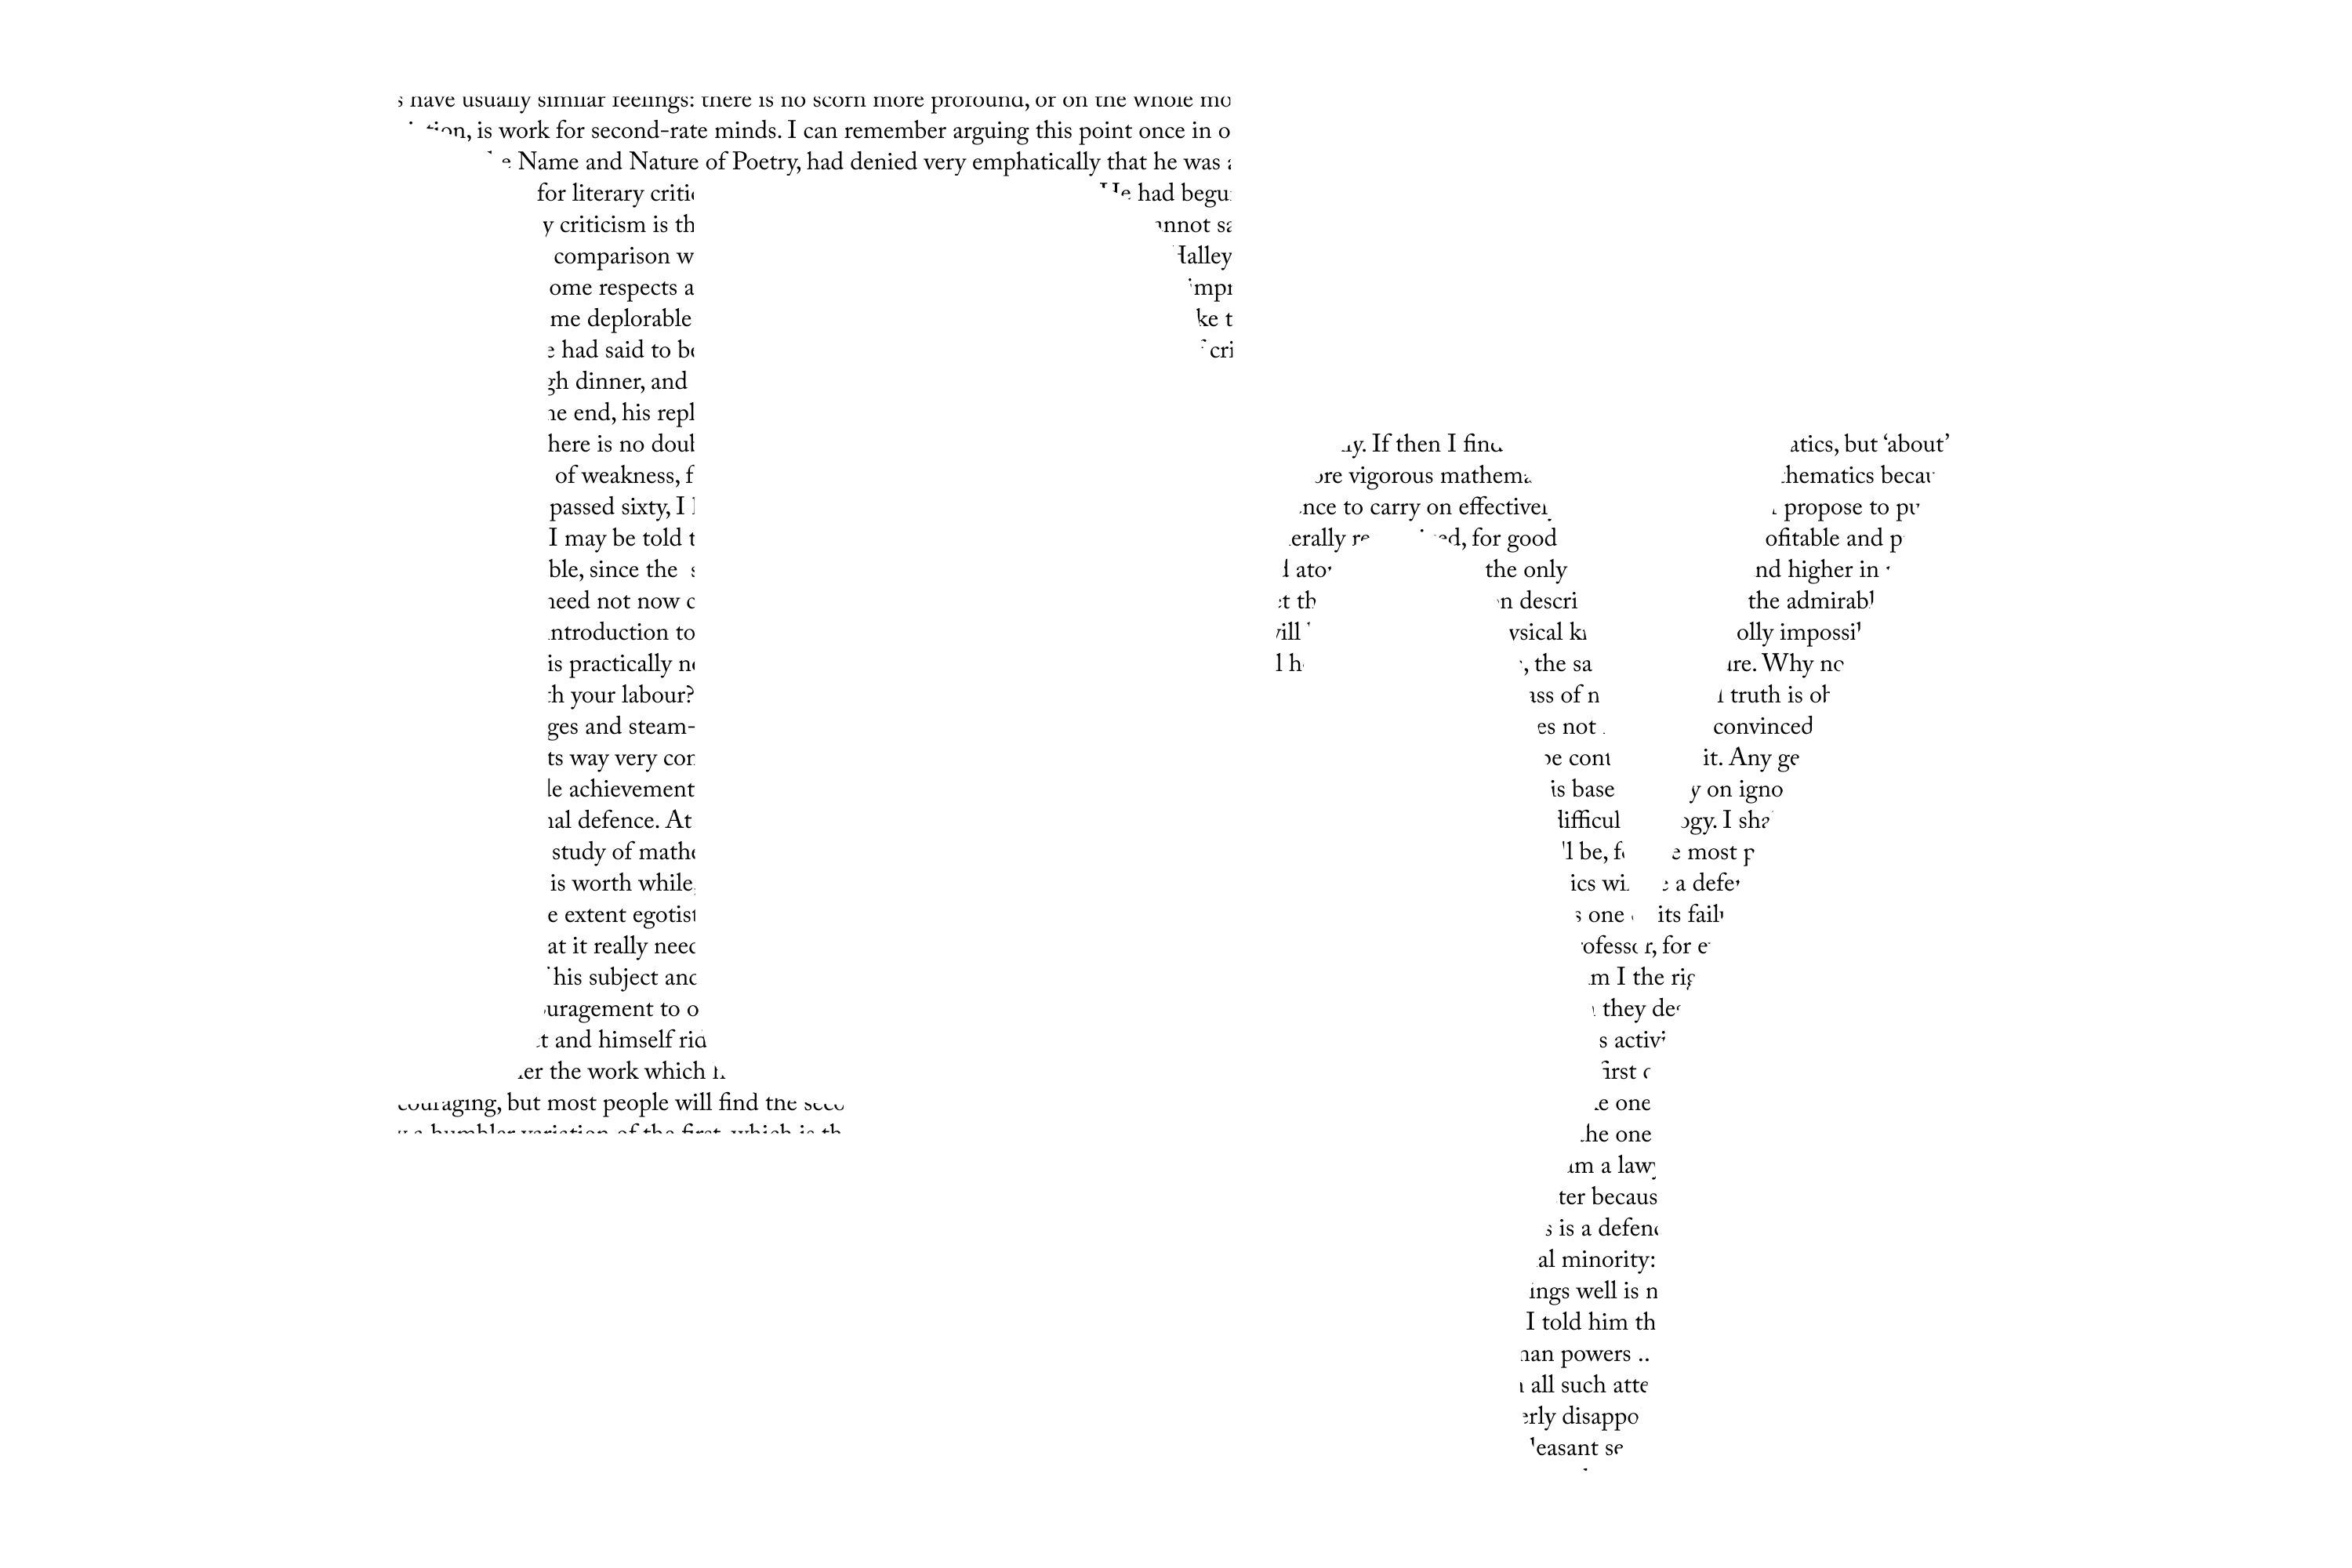
\includegraphics[scale=0.25]{immagini/gamma_illustrata.png}
	\end{figure}
	\vspace*{\fill}
	\pagestyle{empty}
	\begin{appendices}
		\pagestyle{fancy}
		\fancyhead[LO]{\textbf{\thepage}}  % Numero di pagina in grassetto a sinistra
		\fancyhead[RO]{\nouppercase\rightmark}         % Capitolo e sezione a destra

		% Definizione dell'intestazione per pagine pari (Even)
		\fancyhead[LE]{\nouppercase\leftmark}          % Capitolo e sezione a sinistra
		\fancyhead[RE]{\textbf{\thepage}}  % Numero di pagina in grassetto a destra

		% Cancella il footer
		\fancyfoot{}
		\setlength{\headheight}{14.49998pt}
		\addtolength{\topmargin}{-2.49998pt}
		% Personalizzazione della linea orizzontale
		\renewcommand{\headrulewidth}{0.4pt}
		\renewcommand{\footrulewidth}{0pt}
		\chapter{Notazione multi-indice}

La notazione multi-indice è una notazione matematica che consente di semplificare enormemente la scrittura di formule matematiche. Ciò è possibile \emph{generalizzando} il concetto di indice che passa dall'essere
un semplice "numero" ad una $n-$upla ordinata di indici. Consideriamo $\alpha \in \mathbb{N}^n$, ovvero $\alpha = (\alpha_1, \ldots, \alpha_n)$ come nostro multi-indice, allora possiamo definire una serie di operazioni: la più semplice di tutti, data la natura di spazio vettoriale di cui gode $\mathbb{N}^n$, è sicuramente la somma dei multi-indici:
$$
\forall \alpha, \beta \in \mathbb{N}^n, \alpha \pm \beta = (\alpha_1 \pm \beta_1, \ldots, \alpha_n \pm \beta_n).
$$
Per quanto riguarda i nostri scopi, è utile definire la \emph{norma multi-indice}, il \emph{fattoriale multi-indice} e il \emph{coefficiente multinomiale}:
\begin{definition}[norma multi-indice]
	Sia $\alpha \in \mathbb{N}^n$ allora definiamo la norma multi-indice come
	$$
	|\alpha| = \sum_{i=1}^n \alpha_i
	$$
\end{definition}
\begin{definition}[fattoriale multi-indice]
	Sia $\alpha \in \mathbb{N}^n$, definiamo il fattoriale multi-indice di $\alpha$ come
	$$
	\alpha! = \alpha_1 ! \alpha_2 ! \ldots \alpha_n !
	$$
\end{definition}
\begin{definition}[coefficiente multinomiale]
	Sia $\alpha \in \mathbb{N}^n$ tale che $|\alpha| = k$, allora definiamo il coefficiente multinomiale come
	$$
	\binom{k}{\bm{\alpha}} = \frac{k!}{\alpha!} = \frac{k!}{\alpha_1 ! \alpha_2 ! \ldots \alpha_n !}
	$$
\end{definition}
\textbf{Notazione}: per distinguerlo dal normale coefficiente binomiale, nel caso del coefficiente multinomiale, metterò in grassetto il multi-indice.
\begin{remark}
	Potremmo pensino introdurre un ordinamento parziale (ma non è di grande interesse) dicendo che $\alpha \leq \beta \iff \alpha_i \leq \beta_i \, \, \forall i \in \{1, \ldots, n \}$. Si vede subito che, così come è stato definito, questo non può essere un ordinamento totale
\end{remark}
Vediamo come questa notazione può agevolarci la scrittura del polinomio di Taylor e la scrittura dei polinomi in $n$-variabili. Innanzitutto definiamo
\begin{definition}[potenza multi-indice]
	Sia $x \in \mathbb{R}^n$ allora
	\begin{align*}
		x^{\alpha} = x_1^{\alpha_1} x_2^{\alpha_2} \ldots x_n^{\alpha_n}
	\end{align*}
\end{definition}
Questa notazione facilita enormemente la scrittura dei polinomi in $n-$variabili, infatti
\begin{definition}[polinomio in $n-$variabili]
	$P: \mathbb{R}^n \to \mathbb{R}$ è un polinomio in $n-$variabili di grado $k \geq 0$ se
	$$
	\exists C = \{c_\alpha : |\alpha| \leq k, \alpha \in \mathbb{N}^n \} \subset \mathbb{R} 
	$$
	dove $0 \neq c_\beta \in C$ e $|\beta| = k$. Allora
	$$
	P(x) = \sum_{|\alpha| \leq k} c_\alpha x^{\alpha}
	$$
\end{definition}
Oltre a questo possiamo definire la derivata multi-indice
\begin{definition}[derivata multi-indice]
	Sia $\alpha \in \mathbb{N}^n$ allora 
	$$
	\partial^{\alpha}_x = \partial_{x_1}^{\alpha_1} \ldots \partial_{x_n}^{\alpha_n}
	$$
	dove, naturalmente, poniamo che $\partial_{x_j}^0 = 1$
\end{definition}
Riprendiamo il polinomio di Taylor: da quanto visto nella sezione \ref{sec:polinomio_taylor} abbiamo visto che possiamo scrivere il polinomio di Taylor di una funzione $f: \mathbb{R}^n \to \mathbb{R}$ come
$$
P_k(f, \xi)\sum_{i_1, \ldots, i_k=1}^k \partial_{x_{i_1}} \ldots \partial_{x_{i_k}} f(\xi) (x_{i_1} - \xi_{i_1}) \ldots (x_{i_k} - \xi_{i_k}).
$$
Osserviamo che possiamo allora usare la potenza multi-indice per scrivere i termini $(x_{i_j} - \xi_{i_j})$, considerando $\alpha \in \mathbb{N}^n$ e osservando che $\alpha_{j_1}, \ldots, \alpha_{j_m} \geq 1$ e $1 \leq j_1, \ldots, j_m \leq n$ tali che $\alpha_{j_1} + \ldots + \alpha_{j_m} = k$. In altre parole avremo solamente le derivate di ordine superiore
$$
\partial_{x_{j_1}}^{\alpha_{j_1}} \partial_{x_{j_2}}^{\alpha_{j_2}} \ldots \partial_{x_{j_m}}^{\alpha_{j_m}} f(\xi)
$$
e $\alpha_i = 0$ se $i \neq j_1, \ldots, j_m$. \\
Adesso ricordiamo che il teorema di Schwarz ci assicura che la derivata di una funzione di ordine $C^k$ rispetto agli indici $\alpha_{j_1}, \ldots, \alpha_{j_m}$ (rispetto, naturalmente, in ordine a $x_{j_1}, \ldots, x_{j_m}$) è pari a quella ottenuta con una permutazione $\sigma$ degli indici $\alpha_{j_1}, \ldots, \alpha_{j_m}$, dunque dobbiamo moltiplicare i termini della serie di Taylor per un termine che ci "tronca" i termini uguali (si ricordi la dimostrazione della proposizione \ref{prop:caratterizzazione_taylor}, dove compariva il termine $l!$). La possibilità di avere $\alpha_{j_1}$ derivate rispetto a $x_{j_1}$ sulle $k$ possibili è pari a $\binom{k}{\alpha_{j_1}}$ (non siamo interessati all'ordine, dunque usiamo per questo il coefficiente binomiale) e la stessa cosa vale per tutti gli altri termini, infatti
le possibilità di avere $\alpha_{j_2}$ derivate rispetto a $x_{j_2}$ sulle $k-\alpha_{j_1}$ rimanenti è pari a $\binom{k - \alpha_{j_1}}{\alpha_{j_2}}$ e così via. In generale, il numero di modi in cui possiamo distribuire le derivate è pari a
\begin{flalign*}
&\binom{k}{\alpha_{j_1}} \binom{k - \alpha_{j_1}}{\alpha_{j_2}} \ldots \binom{k - \alpha_{j_1} - \ldots - \alpha_{j_{m-1}}}{\alpha_{j_m}} = \frac{k!}{\alpha_{j_1}! (k - \alpha_{j_1})} \frac{(k-\alpha_{j_1})!}{\alpha_{j_2}!(k - \alpha_{j_1} - \alpha_{j_2})!} \frac{(k - \alpha_{j_1} - \alpha_{j_2})!}{\alpha_{j_3}! (k - \alpha_{j_1} - \alpha_{j_2} - \alpha_{j_3})!} \ldots & &\\
&\cdot \frac{(k - \alpha_{j_1} - \ldots - \alpha_{j_{m-2}})!}{\alpha_{j_{m-1}}! (k - \alpha_{j_1} \ldots - \alpha_{j_{m-1}})!} \frac{\alpha_{j_m}}{\alpha_{j_m}! 0!} = \frac{k!}{\alpha_{j_1}! \alpha_{j_2}! \ldots \alpha_{j_m}!} = \binom{k}{\bm{\alpha}}
\end{flalign*}
Con gli argomenti precedenti in combinazione con il teorema di Schwarz di ordine superiore, possiamo dunque dimostrare il seguente lemma
\begin{lemma}
	Sia $f \in C^k(\Omega)$ e $\xi \in \Omega$, allora abbiamo
	$$
	d^l f(\xi)(x - \xi) = \sum_{|\alpha|=l} \binom{l}{\bm{\alpha}} \partial^{\alpha} f(\xi) (x - \xi)^{\alpha}.
	$$
\end{lemma}
\begin{prop}
	Se $f \in C^k(\Omega), \Omega \subseteq \mathbb{R}^n$ aperto e $\xi \in \Omega$, allora abbiamo che
	$$
	P_k(f, \xi)(x) = \sum_{|\alpha| \leq k} \frac{1}{\alpha!} \partial^{\alpha} f(\xi) (x - \xi)^{\alpha}
	$$
\end{prop}
\begin{proof}
	Sappiamo che per $0 \leq j \leq k$ abbiamo che
	$$
	d^j f(\xi)(h) = \sum_{|\alpha| = j} \binom{j}{\bm{\alpha}} \partial^{\alpha} f(\xi) h^{\alpha}
	$$
	e ciò implica, per quanto visto nel capitolo 3, che
	\begin{align*}
	&P_k(f, \xi) = \sum_{j=0}^k \frac{1}{j!} d^j f(\xi)(x - \xi) = \sum_{j=0}^k \sum_{|\alpha| = j} \binom{j}{\bm{\alpha}} \partial^{\alpha}_x f(\xi) (x - \xi)^{\alpha} \stackrel{\binom{j}{\bm{\alpha}} = \frac{j!}{\alpha!}}{=} \sum_{j=0}^k \sum_{|\alpha| = j} \frac{1}{\alpha!} \partial^{\alpha}_x f(\xi) (x - \xi)^{\alpha} = & &\\
	&= \sum_{0 \leq |\alpha| \leq k} \frac{1}{\alpha!} \partial^{\alpha}_x f(\xi) (x - \xi)^{\alpha}
	\end{align*}
\end{proof}
\begin{theorem}[formula di Taylor coi multi-indici]
	Se $f \in C^k(\Omega), \xi \in \Omega, \Omega \subseteq \mathbb{R}^n$ aperto, allora abbiamo che
	$$
	f(x) = \sum_{0 \leq |\alpha| \leq k} \frac{1}{\alpha!} \partial_x^{\alpha} f(\xi) (x - \xi)^{\alpha} + o(|x-\xi|^{\alpha})
	$$
\end{theorem}
\begin{proof}
	La dimostrazione segue dalla precedente proposizione e dalla formula di Taylor che abbiamo visto nel capitolo 3.
\end{proof}
		\chapter{Dimostrazione del teorema della funzione inversa}
\pagestyle{plain}
\thispagestyle{empty}
\pagestyle{fancy}
In questa appendice ci proponiamo di dimostrare in maniera rigorosa il teorema della funzione inversa, riportando tutti i teoremi precedentemente non enunciati necessari per effettuare la dimostrazione. Sarebbe anche interessante mostrare che il teorema del Dini implica il teorema della funzione inversa, mostrando così
che i due teoremi sono equivalenti, tuttavia ciò non verrà fatto.

\begin{theorem}[della funzione inversa]
    Sia $\Omega \subseteq \mathbb{R}^n$ aperto, $f \in C^k(\Omega, \mathbb{R}^n), x_0 \in \Omega$ e $Df(x_0) \in \mathbb{R}^{n \times n}$ invertibile. \\
    Allora $\exists \rho > 0: \exists U \subseteq \mathbb{R}^n$ aperto tali che $f_{|_{B(x_0, \rho)}} \in C^{k}(B(x_0, \rho), U)$ è invertibile e, posto $g=(f_{|_{B(x_0, \rho)}})^{-1}:U \to B(x_0, \rho)$, abbiamo che
    $g \in C^k(U, B(x_0, \rho))$ con
    $$
    Dg(y) = (Df(g(y)))^{-1} \, \forall y \in U
    $$
    \label{thm:inverse_function}
    \end{theorem}

\section{Norma matriciale indotta}

Per dimostrare questo risultato, è conveniente passare ad una norma differente di quella di Hilbert-Schmidt. Sebbene tutte le norme, in uno spazio finito dimensionale sono equivalenti (e dunque inducono la stessa topologia) l'utilizzo di questa norma rende più semplice la trattazione
di alcuni risultati di cui abbiamo bisogno. Iniziamo dando la definizione di spazio delle applicazione lineari fra due spazi vettoriali, la quale dovrebbe già essere stata data nel corso di Geometria, che riporto per completezza
\begin{definition}[spazio delle applicazioni lineari]
    Siano $X, Y$ due spazi vettoriali su un campo $\mathbb{K}$. Definiamo
    $$
    \mathcal{L}(X, Y) = \{f: X \mapsto Y \, | \, f \text{ è lineare} \}
    $$
\end{definition}
\begin{remark}
    Se $A : \mathbb{R}^n \mapsto \mathbb{R}^n$ lineare, scriveremo che $A \in \mathcal{L}(\mathbb{R}^n)$
\end{remark}
\begin{remark}
    $\mathcal{L}(X, Y)$ con $X, Y$ spazi vettoriali su un campo $\mathbb{K}$ è uno spazio vettoriale
\end{remark}
\begin{definition}[norma matriciale indotta]
    Sia $A \in \mathcal{L}(\mathbb{R}^n, \mathbb{R}^m)$, allora definiamo la norma $|| A ||$ matriciale di A come
    \begin{equation}
        || A || = \sup_{x \in \mathbb{S}^{n-1}} |Ax|
    \end{equation}
    dove $|\cdot|:\mathbb{R}^m \to \mathbb{R}$ è la usuale norma euclidea.
\end{definition}
\begin{remark}
    Questa norma viene chiamata, in maniera suggestiva, \emph{indotta} siccome non è altro che la norma vettoriale utilizzata in $\mathbb{R}^n$ che viene "indotta" sullo spazio delle matrici considerando il $\sup$ della norma euclidea della matrice applicata sui vettori di norma $1$.
\end{remark}
\begin{remark}
    Si potrebbero definire le $p-$norme indotte, definite nell'usuale maniera riportata sopra, dove si utilizza come norma vettoriale la norma $|| \cdot ||_p \, : \mathbb{R}^n \to \mathbb{R}$ tale che
    $$
    (x_1, \ldots, x_n) \stackrel{||\cdot||_p}{\mapsto} \left( \sum_{i=1}^n |x_i|^p \right)^{\frac{1}{p}}
    $$
\end{remark}
\begin{remark}
    Osserviamo che
    \begin{equation}
    |Ax| \leq || A || \, |x|
    \label{eq:matrix_norm_inequality}
    \end{equation}
    vale $\forall x \in \mathbb{R}^n$. Inoltre, se $\exists \lambda \in \mathbb{R} : \forall x \in \mathbb{R}^n, |Ax| \leq \lambda |x|$ allora $|| A || \leq \lambda$
\end{remark}
\begin{exercise}
    Mostrare la disuguaglianza (\ref{eq:matrix_norm_inequality}).
\end{exercise}
\begin{proof}[Svolgimento]
    Sia $x \in \mathbb{R}^n$. Allora sappiamo che
    $$
    |Ax| = \big|A( \, |x| \, \frac{x}{|x|} )\big| = |x| \, \big|A\frac{x}{|x|}\big| \leq |x| \, || A ||
    $$
    siccome $\frac{x}{|x|}$ è un vettore di norma unitaria.
\end{proof}
Per pura completezza, riporto la dimostrazione che due norme, nel caso finito-dimensionale, sono \emph{equivalenti}
\begin{definition}[equivalenza fra norme]
    Sia $V$ un $\mathbb{K}-$spazio vettoriale e siano $||\cdot||_1, ||\cdot||_2$ due norme definite sullo spazio vettoriale. Allora diremo che esse sono equivalenti se esistono due costanti $c$ e $C$ strettamente positive per cui
    \begin{equation}
        \forall x \in V, c||x||_1 \leq ||x||_2 \leq C||x||_1.
    \end{equation}
\end{definition}
\begin{remark}
    Due norme equivalenti inducono la stessa topologia (impropriamente la stessa metrica), quindi strutture topologiche quali gli insiemi aperti, le funzioni continue e successioni convergenti rimarrano tali "cambiando" norma: questo potrà sembrare di poco conto e un'astrazione non necessaria, tuttavia, ripensando a come abbiamo costruito tutta la teoria dei limiti e delle successioni in $\mathbb{R}^n$, ci accorgiamo che la norma è l'oggetto su cui abbiamo basato la nostra nozione di convergenza. Dire che
    due norme inducono la stessa topologia vuol dire che presi due oggetti $x, y \in \mathbb{R}^n$ tali che $|x - y| \to 0$ (dove con $|\cdot|: \mathbb{R}^n \to \mathbb{R}$ intendo la norma euclidea) allora presa una qualunque altra norma $||\cdot||_{\star}: \mathbb{R}^n \to \mathbb{R}$ avremo che $||x - y||_{\star} \to 0$. 
    Questo è un risultato non banale e che, in generale, non è vero per spazi vettoriali infinito-dimensionali.
\end{remark}
\begin{prop}[tutte le norme sono equivalenti a quella euclidea su $\mathbb{R}^n / \, \mathbb{C}^n$]
    Sia $n \in \mathbb{N}$. Tutte le norme su $\mathbb{R}^n$ (o $\mathbb{C}^n$) sono equivalenti alla norma euclidea.
    \label{thm:equiv_norme_euclidea}
\end{prop}
\begin{proof}
    Senza perdita di generalità effettueremo la dimostrazione nel caso di $\mathbb{R}^n$. Sia $|| \cdot ||_{\star}$ una norma su $\mathbb{R}^n$ e denotiamo con $||x||_2$ la norma euclidea. Siano $\{e_1, \ldots, e_n \}$ una base canonica su $\mathbb{R}^n$, allora $\forall x \in \mathbb{R}^n, \exists x_1, x_2, \ldots, x_n \in \mathbb{R}^n : x = x_1 e_1 + \ldots + x_n e_n;$ possiamo allora
    applicare ripetutamente la disuguaglianza triangolare sulla norma di $x$ per minorarla
    $$
    ||x||_{\star} = ||\sum_{i=1}^n x_i e_i ||_{\star} \leq \sum_{i=1}^n ||x_i e_i||_{\star} = \sum_{i=1}^n |x_i| ||e_i||_{\star} \leq \sqrt{\sum_{i=1} |x_i|^2 \sum_{i=1}^n ||e_i||^2_{\star}} = ||x||_2 \sqrt{\sum_{i=1}^n ||e_i||^2_{\star}}.
    $$
    dove nell'ultima minorazione si è utilizzata la disuguaglianza di Cauchy-Schwarz. \\
    Dunque se poniamo $A = \sqrt{\sum\limits_{i=1}^n ||e_i||^2_{\star}}$ otteniamo che $||x||_{\star} \leq A||x||_2 \, \, \forall x \in \mathbb{R}^n$, ovvero la norma euclidea domina la norma $\star$. A questo punto, per vedere che la norma $\star$ domina quella euclidea, possiamo considerare la funzione
    $$
    f(x) = ||x||_{\star}
    $$
    Osserviamo che
    $$
    |f(x) - f(y)| = | \, ||x||_{\star} - ||y||_{\star}| \leq ||x-y||_{\star} \leq A||x-y||_2, \, \, \forall x, y \in \mathbb{R}^n,
    $$
    questo prova che la funzione $f$ è lipschtziana, dunque continua rispetto alla norma euclidea. Consideriamo la sfera unitaria $\mathbb{S}^{n-1}$: tale insieme è infatti compatto per il teorema di Heine-Borel (teorema \ref{thm:heine_borel}) in quanto limitato (banale) e chiuso (corollario del lemma \ref{lemma:frontiera_chiusa} dimostrato più avanti), conseguentemente, avremo per il teorema di Weierstrass (teorema \ref{thm:weierstrass}) che 
    la funzione $f$ assumerà massimo e minimo. Sia $u_{\star} \in \mathbb{S}^{n-1}$ tale che
    $$
        \min_{u \in \mathbb{S}^{n-1}} ||u||_{\star} = \min_{u \in U} f(u) = f(u_{\star}) = ||u_{\star}||_{\star}.
    $$
    Indichiamo tale risultato con $B = ||u_{\star}||_{\star} > 0$ è strettamente positivo siccome $||v||_{\star} = 0 \iff v = 0$ (una delle proprietà di cui gode la norma) e nel nostro caso stiamo considerando $u \in \mathbb{S}^{n-1} = {u \in \mathbb{R}^n : ||u||_2 = 1}$, dunque $\forall u \in \mathbb{S}^{n-1}, u \neq 0$. Ma allora, per ogni $x$ non nullo abbiamo che
    $$
    ||x||_{\star} = || \, ||x||_2 \, \frac{x}{||x||_2} \, ||_{\star} = ||x||_2 \, || \, \frac{x}{||x||_2} \, ||_{\star} \geq ||x||_2 \, B
    $$
    siccome $\frac{x}{||x||_2}$ è un vettore unitario rispetto alla norma euclidea e, per quanto visto prima, abbiamo che $\forall u \in \mathbb{S}^{n-1}, B = ||u_{\star}||_{\star} \leq ||u||_{\star}$, giustificando così la maggiorazione effettuata nell'ultimo passaggio. Concludendo, abbiamo che
    $$
        B |||x||_2 \leq ||x||_{\star} \leq A ||x||_2
    $$
    e
    $$
        \frac{1}{A} ||x||_{\star} \leq ||x||_2 \leq \frac{1}{B} ||x||_{\star}
    $$
    dunque $||\cdot||_{\star}$ e $||\cdot||_2$ sono equivalenti.
\end{proof}
\begin{cor}[tutte le norme sono equivalenti in $\mathbb{R}^n / \, \mathbb{C}^n$]
    Sia $n \in \mathbb{N}$. Tutte le norme sono equivalenti in $\mathbb{R}^n / \, \mathbb{C}^n$.
\end{cor}
\begin{proof}
    Come visto nella dimostrazione del teorema \ref{thm:equiv_norme_euclidea}, sappiamo che prese due norme $||\cdot||_{\star}$ e $||\cdot||_{\ast}$ avremo che $\exists A_{\star}, B_{\star}, A_{\ast}, B_{\ast} \in \mathbb{R}$ tali che
    \begin{align*}
        &B_{\star} \, ||x||_2 \leq ||x||_{\star} \leq A_{\star} \, ||x||_2 & &B_{\ast} \, ||x||_2 \leq ||x||_{\ast} \leq A_{\ast} \, ||x||_2 \\
        &\frac{1}{A_{\star}} \, ||x||_{\star} \leq ||x||_{2} \leq \frac{1}{B_{\star}} ||x||_{\star} & &\frac{1}{A_{\ast}} \, ||x||_{\ast} \leq ||x||_{2} \leq \frac{1}{B_{\ast}} ||x||_{\ast}
    \end{align*}
    pertanto abbiamo che
    $$
    ||x||_{\ast} \leq  A_{\ast} \, ||x||_2 = \frac{A_{\ast}}{B_{\star}} B_{\star} \, ||x||_2 \leq \frac{A_{\ast}}{B_{\star}} \, ||x||_{\star} \implies ||x||_{\ast} \leq \frac{A_{\ast}}{B_{\star}} \, ||x||_{\star}
    $$
    e similmente possiamo vedere che
    $$
    ||x||_{\ast} \geq B_{\ast} ||x||_2 = B_{\ast} \frac{1}{A_{\star}} ||x||_{\star} \implies ||x||_{\ast} \geq \frac{B_{\ast}}{A_{\star}} ||x||_{\star}.
    $$
    Conseguentemente, si conclude che
    $$
    \frac{B_{\ast}}{A_{\star}} \, ||x||_{\star} \leq ||x||_{\ast} \leq \frac{A_{\ast}}{B_{\star}} \, ||x||_{\star},
    $$
    e
    $$
    \frac{B_{\star}}{A_{\ast}} \, ||x||_{\ast} \leq ||x||_{\star} \leq \frac{A_{\star}}{B_{\ast}} \, ||x||_{\ast}.
    $$
    Dunque le norme $||\cdot||_{\star}$ e $||\cdot||_{\ast}$ sono equivalenti.
\end{proof}
\begin{cor}[tutte le norme sono equivalenti su spazi di dimensione finita]
    Sia $V$ un $\mathbb{R}-$spazio (o un $\mathbb{C}-$spazio) di dimensione finita $n$. Allora tutte le norme sono equivalenti. 
    \label{cor:equivalence_norms}
\end{cor}
\begin{proof}
    Senza perdita di generalità faremo la dimostrazione nel caso di $\mathbb{R}-$spazio vettoriale. Sia $(V, ||\cdot||_V)$ uno spazio vettoriale normato reale di dimensione finita $n$ e fissiamo una base $\mathcal{B} = \{ v_1, \ldots, v_n \}$ di tale spazio.
    Sappiamo allora che $\forall v \in V \exists \lambda \in \mathbb{R}^n : v = \sum_{i=1}^n b_i v_i$ con $\lambda = (\lambda_1, \ldots, \lambda_n)$: possiamo dunque considerare l'isomorfismo lineare
    \begin{align*}
        &\phi: \mathbb{R}^n \to V \, \, \text{tale che} \, \, \lambda \in \mathbb{R}^n \stackrel{\phi}{\mapsto} \sum_{i=1}^n \lambda_i v_i \in V.
    \end{align*}
    Grazie a questo isomorfismo possiamo far corrispondere alla norma di $V$ una norma definita su $\mathbb{R}^n$ definita come
    $$
    ||\lambda||_{\star} = ||\phi(\lambda)||_V, \, \, \forall \lambda \in \mathbb{R}^n.
    $$
    Verifichiamo che essa è una norma su $\mathbb{R}^n$: abbiamo che $\phi(\lambda) = 0_V \iff \lambda = \underline{0}$ (siccome $\phi$ è un isomorfismo lineare) e per proprietà della norma $||\cdot||_V$ abbiamo che $||v||_V = 0 \iff v = 0$, dunque abbiamo effettivamente che $||\lambda||_{\star} = 0 \iff \lambda = \underline{0}$. Preso adesso uno scalare $c \in \mathbb{R}$ e $\lambda \in \mathbb{R}^n$, abbiamo che
    $\phi(c\lambda) = c\phi(\lambda)$ (sempre perché $\phi$ è un isomorfismo lineare) e, per proprietà di omogeneità della norma, abbiamo che $||c\lambda||_{\star} = ||\phi(c\lambda)||_V = ||c \phi(\lambda) ||_V = |c| \, ||\phi(\lambda)||_V = |c| \, ||\lambda||_{\star}$, mentre per la disuguaglianza triangolare abbiamo che presi $\lambda_1, \lambda_2 \in \mathbb{R}^n$ abbiamo che
    $$
        ||\lambda_1 + \lambda_2||_{\star} = ||\phi(\lambda_1 + \lambda_2)||_V \leq ||\phi(\lambda_1)||_V + ||\phi(\lambda_2)||_V = ||\lambda_1||_{\star} + ||\lambda_2||_{\star},
    $$
    dove nei passaggio abbiamo utilizzato che $\phi(\lambda_1 + \lambda_2) = \phi(\lambda_1) + \phi(\lambda_2)$ (sempre perché $\phi$ è un isomorfismo lineare) e la disuguaglianza triangolare di cui gode la norma $||\cdot||_V$. Dunque la norma definita come
    $$
        ||\lambda||_{\star} = ||\phi(\lambda)||_V
    $$
    è una norma su $\mathbb{R}^n$. \\
    Siano adesso $||\cdot||_{\flat\star} = ||\phi(\cdot)||_{\flat}$ e $||\cdot||_{\sharp\star} = ||\phi(\cdot)||_{\sharp}$ due norme su $\mathbb{R}^n$. Per il corollario \ref{cor:equivalence_norms} abbiamo che
    $$
    \exists A_\flat, B_\flat, A_\sharp, B_\sharp \in \mathbb{R} : \begin{cases}
        A_\flat \, ||\lambda||_{\sharp\star} \leq ||\lambda||_{\flat\star} \leq B_\flat \, ||\lambda||_{\sharp\star} \\
        A_\sharp \, ||\lambda||_{\flat\star} \leq ||\lambda||_{\sharp\star} \leq B_\sharp \, ||\lambda||_{\flat\star}
    \end{cases} \, \, \forall \lambda \in \mathbb{R}^n.
    $$
    Ma siccome $\phi$ è un isomorfismo suriettivo allora avremo che
    $$
    \begin{cases}
        A_\flat \, ||v||_{\sharp} \leq ||v||_{\flat} \leq B_\flat \, ||v||_{\sharp} \\
        A_\sharp \, ||v||_{\flat} \leq ||v||_{\sharp} \leq B_\sharp \, ||v||_{\flat}
    \end{cases} \, \, \forall v \in V,
    $$
    ovvero le norme $||\cdot||_{\flat}$ e $||\cdot||_{\sharp}$ sono equivalenti.
\end{proof}
\section{Alcuni risulti preliminari per la dimostrazione}

Andiamo ad enunciare alcuni risultati di cui abbiamo bisogno per dimostrare quanto ci siamo prefissi all'inizio di questa appendice. Alcuni di essi dovrebbero essere già noti dal corso di Analisi Matematica:
\begin{theorem}[di Banach-Caccioppoli]
	Sia $X$ uno spazio metrico completo e sia $\varphi: X \to X$ una contrazione (ovvero una funzione $L-$lipschtziana con $L < 1$). Allora $\exists ! x \in X : \varphi(x) = x$
\end{theorem}
\begin{proof}
	Sia $(X, d)$ uno spazio metrico completo e sia $x_0 \in X$. Definiamo una successione $\{ x_n \}$ in maniera ricorsiva, imponendo che
	\begin{align*}
		&x_{n+1} = \varphi(x_n) & &(n = 0, 1, \ldots).
	\end{align*}
	La dimostrazione segue in due \emph{step}: la prima consiste nel mostrare l'esistenza di un punto fisso, la seconda l'unicità di tale punto. \\
	\emph{Esistenza}: l'idea è quella di mostrare che questa successione da noi definita è una successione di Cauchy, da cui segue, data la completezza di $X$, che la successione converge a $x \in X$. \\
	Siccome $\varphi$ è una contrazione, allora $\exists c \in \mathbb{R}$ tale che $c < 1$ e $\forall x, y \in X, d(\varphi(x), \varphi(y)) \leq c d(x, y)$. Dunque avremo che
	$$
	d(x_{n+1}, x_n) = d(\varphi(x_n), \varphi(x_{n-1})) \leq c d(x_n, x_{n-1})
	$$
	Procedendo induttivamente (il caso $n=1$ è naturalmente banale) avremo che
	$$
	d(x_{n+1}, x_n) \leq c d(x_n, x_{n-1}) \leq c^n d(x_1, x_0)
	$$
	mentre se prendiamo $n \neq m$ e supponiamo (senza perdere di generalità) che $n > m$ allora
	\begin{align*}
	d(x_n, x_m) &\stackrel{\text{dis. triang.}}{\leq} \sum_{i = m}^{n-1} d(x_i, x_{i+1}) \leq \sum_{i=m}^{n-1} c^{i} d(x_1, x_0) = d(x_1, x_0) \sum_{i=m}^{n+1} c^{i} = \\
	&= d(x_1, x_0) \left( \frac{1-c^{n+1}}{1-c} - \frac{1 - c^{m+1}}{1-c} \right) = \frac{c^{m} - c^{n}}{1-c} d(x_1, x_0).
	\end{align*}
	Ma, siccome $c < 1$, se $m \to +\infty$ e $n > m$ allora quest'ultima quantità tende a $0$, dunque risulta che $\{ x_n \}$ è una successione di Cauchy. Conseguentemente, essendo $X$ completo,
	tale successione converge ad un punto $x \in X$ e, usando la continuità di $\varphi$, abbiamo che
	$$
	x_{k+1} = \varphi(x_k) \implies \lim_{k \to +\infty} x_{k+1} = \lim_{x \to +\infty} \varphi(x_k) \implies x = \varphi(x).
	$$
	\emph{Unicità}: supponiamo per assurdo che esistano due punti fissi, ovvero $\exists x, y \in X, x \neq y : \varphi(x) = x, \varphi(y) = y$. Allora avremo che
	$$
	d(x, y) = d(\varphi(x), \varphi(y)) \leq c d(x, y) \implies d(x, y) \leq c d(x, y) \implies c > 1
	$$
	il che è un assurdo siccome $\varphi$ è una contrazione.
\end{proof}
\begin{theorem}[criterio di Lipschtiz]
	Sia $\Omega \subseteq \mathbb{R}^n$ convesso, $f: \Omega \to \mathbb{R}^m$ una funzione di classe $C^1(\Omega, \mathbb{R}^m)$ e supponiamo che si abbia $L = \sup\limits_{x \in \Omega} ||Df(x)|| < +\infty$. Allora la funzione
	$f$ è $L-$lipschtziana, ossia
	$$
	\forall x, y \in \Omega, |f(x) - f(y)| \leq L|x-y|
	$$
\end{theorem}
\begin{proof}
	Fissiamo $x, x' \in \Omega$, allora consideriamo la funzione $g(t) = f(tx + (1-t)y)$ con $t \in [0, 1]$, pertanto $g: [0, 1] \to \mathbb{R}^m$ ed è anch'essa di classe $C^1$ e si ha che
	$$
	g'(t) = Df(tx + (1-t)y)(x - y)
	$$
	e, dalla formula fondamentale del calcolo integrale, segue che 
	$$
	f(x) - f(y) = g(1) - g(0) = \int_0^1 g'(t)dt = \int_0^1 Df(tx + (1-t)y)(x-y)dt
	$$
	da cui segue che
	\begin{align*}
	|f(x) - f(y)| = |\int_0^1 Df(tx + (1-t)y)(x-y)dt| &\leq \int_0^1 || Df(tx + (1-t)y) || |x-y|dt \leq \\
	&\leq \int_0^1 Ldt |x-y| = L|x-y|
	\end{align*}
\end{proof}
\begin{lemma}
    $\forall n > 0, \forall r > 0, \forall x \in \mathbb{R}^n, B_r(x) \subset \mathbb{R}^n$ sono convesse.
\end{lemma}
\begin{proof}
    Fissiamo $n > 0$, $r > 0$ e $x \in \mathbb{R}^n$. Siano adesso $y, z \in B_r(x)$ e consideriamo il luogo dei punti descritti da
    $$
    \alpha = ty + (1-t)z, \text{ con } t \in [0, 1].
    $$
    Allora
    \begin{align*}
    | \alpha - x | &= |ty + (1-t)z - x| \leq |ty + (1-t)z - tx - (1 - t)x| \leq |ty - tx| + |(1-t)z - (1-t)x| = \\
    &=t \, |y - x| + (1-t) \, |z - x| < tr + (1-t)r = r 
    \end{align*}
\end{proof}
\begin{remark}
    Questa dimostrazione è valida, in realtà, per ogni spazio vettoriale munito di norma. Il fatto che le palle siano convesse non è valido per ogni spazio metrico: un esempio può essere dato da $\mathbb{R}^2$ munito della distanza
    $$
    d((x_1, x_2), (y_1, y_2)) = \sqrt{|x_1 - y_1|} + \sqrt{|x_2 - y_2|}
    $$
    dove la palla centrata in $(0, 0)$ e di raggio $1$ assume la seguente forma
    
    \begin{figure}[H]
        \centering
        \scalebox{1.5}{\begin{tikzpicture}
            % Imposta l'area del luogo geometrico
            \fill[blue!20, domain=0:1, samples=200, smooth]
                plot[samples=200, domain=0:1] ({\x^2}, {(1-\x)^2}) -- % Primo quadrante
                plot[samples=200, domain=0:1] ({-(1-\x)^2}, {\x^2}) -- % Secondo quadrante
                plot[samples=200, domain=0:1] ({-\x^2}, {-(1-\x)^2}) -- % Terzo quadrante
                plot[samples=200, domain=0:1] ({(1-\x)^2}, {-\x^2}) -- cycle; % Quarto quadrante
        
            % Disegna il bordo del luogo geometrico
            \draw[thick, blue, smooth, domain=0:1]
                plot[samples=200] ({\x^2}, {(1-\x)^2}) -- % Primo quadrante
                plot[samples=200] ({-(1-\x)^2}, {\x^2}) -- % Secondo quadrante
                plot[samples=200] ({-\x^2}, {-(1-\x)^2}) -- % Terzo quadrante
                plot[samples=200] ({(1-\x)^2}, {-\x^2}) -- cycle; % Quarto quadrante
        
            % Disegna gli assi
            \draw[->] (-1, 0) -- (1, 0);
            \draw[->] (0, -1) -- (0, 1);
        \end{tikzpicture}}
    \end{figure}
\end{remark}
Nel prossimo teorema facciamo uso del seguente risultato che propongo come esercizio
\begin{exercise}
    Sia $A \in \mathcal{L}(\mathbb{R}^n, \mathbb{R}^m)$ e sia $B \in \mathcal{L}(\mathbb{R}^m, \mathbb{R}^k)$, allora
    $$
        || BA || \leq || B || \, || A ||.
    $$
    Mostrare questo risultato sia per la norma matriciale indotta che per la norma di Hilbert-Schmidt
\end{exercise}
\begin{proof}[Svolgimento]
    Nel caso della norma matriciale indotta abbiamo che
    $$
    || BAx || \leq || B(Ax) || \leq || B || |Ax| \leq || B || \, || A || \, |x| \implies || BA || \leq || B || \, || A ||
    $$
    dove abbiamo utilizzato ripetutamente la (\ref{eq:matrix_norm_inequality}). \\
    Per quanto riguarda la norma di Hilbert-Schmidt, osserviamo che, posto $C = BA$, abbiamo che
    \begin{align*}
    || C || = \sqrt{\sum_{i, j} c_{ij}^2} &= \sqrt{\sum_{i}^k \sum_j^n \left( \sum_{k=1} a_{ik} b_{kj} \right)^2} \leq \sqrt{\sum_{i}^k \sum_j^n \sum_{l=1}^m a_{il}^2 \sum_{l=1}^m b_{lj}^2} = \\
    &= \sqrt{\sum_i^k \sum_{l}^m a_{il}^2 \sum_{j}^n \sum_{l}^m b_{lj}^2} = \sqrt{\sum_{i, l} a_{il}^2 \sum_{l, j} b_{lj}^2} = || B || \, || A ||
    \end{align*}
    dove abbiamo utilizzato la disuguaglianza di Cauchy-Schwarz per giustificare la minorazione. Dunque
    $$
    || BA || \leq || B || \, || A ||.
    $$
\end{proof}
\begin{theorem}[continuità dell'operazione di inversione di una matrice]
    Sia $\mathit{\Omega}$ l'insieme di tutte le applicazioni lineari invertibili a valori in $\mathbb{R}^n$. Allora
    \begin{enumerate}[label=\protect\circled{\arabic*}]
        \item Se $A \in \mathit{\Omega}$, $B \in \mathcal{L}(\mathbb{R}^n)$ e
        \begin{equation*}
            || B - A || \cdot || A^{-1} || < 1 \tag{$\ast$}
        \end{equation*}
        allora $B \in \mathit{\Omega}$.
        \item $\mathit{\Omega}$ è un insieme aperto di $\mathcal{L}(R^n)$ e la mappa $A \mapsto A^{-1}$ è continua su $\mathit{\Omega}$ 
    \end{enumerate}
    \label{thm:continuity_of_the_inverse_matrix}
\end{theorem}
\begin{proof}
Mostriamo la \circled{1}. Osserviamo che prese $A \in \mathit{\Omega}, B \in \mathcal{L}(\mathbb{R}^n)$ che soddisfano la ($\ast$) e, per comodità, poniamo $\frac{1}{\alpha} = || A^{-1} ||$ e $|| B - A || = \beta$. Dunque la ($\ast$) diventa
$$
\frac{\beta}{\alpha} < 1 \implies \alpha > \beta.
$$
Osserviamo adesso che $\forall x \in \mathbb{R}^n$
$$
\alpha |x| = \alpha | A^{-1} A x | \leq \alpha || A^{-1} || \, |Ax| = |Ax| = |(A - B + B)x| \leq |(A-B)x| + |Bx| \leq \beta |x| + |Bx|
$$
dunque
\begin{equation*}
0 \leq (\alpha - \beta) |x| \leq |Bx| \tag{\text{$\star$}}
\end{equation*}
dove la prima eguaglianza segue dal fatto che $\alpha - \beta > 0$. Ma questo allora implica che $Bx \neq 0$ se $x \neq \underline{0}$: questo ci permette di concludere, per una serie di noti risultati visti dal corso di Geometria, che $B$ è un isomorfismo, dunque è invertibile, quindi $B \in \mathit{\Omega}$. \\
Mostriamo la \circled{2}. Prendiamo $x = B^{-1}y$ e mettiamola all'interno della ($\star$)
$$
(\alpha - \beta) |B^{-1}y| \leq |BB^{-1}y| = |y|
$$
che una relazione valida $\forall y \in \mathbb{R}^n$ da cui possiamo dedurre che
$$
    |B^{-1}y| \leq \frac{1}{\alpha - \beta} |y| \implies || B || \leq \frac{1}{\alpha - \beta}.
$$
Osservando che
$$
    B^{-1} - A^{-1} = B^{-1} (A-B) A^{-1}
$$
abbiamo che
$$
|| B^{-1} - A^{-1} || \leq || B^{-1} || \, || A - B || \, || A^{-1} || \leq \frac{1}{\alpha - \beta} \frac{\beta}{\alpha} = \frac{\beta}{\alpha (\alpha - \beta)}
$$
e per $\beta \to 0$ osserviamo che $|| B - A || \to 0$, dunque la mappa che associa ad una matrice la sua inversa è continua.
\end{proof}
\begin{remark}
    Il passaggio in cui abbiamo affermato che $|| B || \leq \frac{1}{\alpha - \beta}$ sarebbe fallito con la norma di Hilbert-Schmidt. Sarebbe invece stato corretto nel caso in cui io avessi affermato che $|| B || \leq \frac{\sqrt{N}}{\alpha - \beta}$: il motivo
    di questo deriva dal fatto che in base ortonormale la norma di Hilbert-Schmidt altro non è che $|| B || = \sqrt{\sum\limits_{i=1}^n |Be_i|^2}$ dove $\{e_1, \ldots, e_n \}$ è una qualunque base ortonormale dello spazio vettoriale su cui mi trovo e $|\cdot|:V \to \mathbb{K}$ è la norma su essa definita. Nel caso sopra se risultava che
    $|Bx| \leq \frac{1}{\alpha - \beta} |x| \, \, \forall x \in \mathbb{R}^n \implies |Be_i| < \frac{1}{\alpha - \beta} \implies || B || = \sqrt{\sum\limits_{i=1}^n |Be_i|^2} \leq \sqrt{\sum\limits_{i=1}^n \frac{1}{(\alpha - \beta)^2}} = \frac{\sqrt{N}}{\alpha - \beta}$. Siccome queste dimostrazioni risultano più naturali con la norma matriciale indotta, ho preferito
    passare a questa norma piuttosto che rimanere con quella di Hilbert-Schmidt, sebbene, in linea di principio, queste dimostrazioni si potrebbero "riadattare" siccome le due norme sono equivalenti.
\end{remark}
\begin{lemma}
    $\forall \Omega \subseteq \mathbb{R}^n, \text{Fr} \, \Omega$ è un insieme chiuso.
    \label{lemma:frontiera_chiusa}
\end{lemma}
\begin{proof}
    La dimostrazione è immediata: sappiamo dall'esercizio \ref{exercise:frontiera_intersec} che la frontiera di $\Omega$ è definita come $\text{Fr} \, \Omega = \overline{\Omega} \cap \overline{\Omega^c}$. Conseguentemente,
    abbiamo che $\overline{\Omega}$ è un insieme chiuso, $\overline{\Omega^c}$ è chiuso e abbiamo che
    $$
        (\overline{\Omega} \cap \overline{\Omega^c})^c = (\mathbb{R}^n \setminus \overline{\Omega}) \cup (\mathbb{R}^n \setminus \overline{\Omega^c})
    $$
    ma, per quanto mostrato nella proposizione \ref{prop:set_closed_iff_compl_open}, abbiamo che $\mathbb{R}^n \setminus \overline{\Omega}$ e $\mathbb{R}^n \setminus \overline{\Omega^c}$ sono insiemi aperti e, per quanto visto nell'esercizio \ref{exercise:union_open_set_is_open}, abbiamo che
    l'unione di insiemi aperti è un insieme aperto. Ma allora il complementare di $\text{Fr} \, \Omega$ è aperto, dunque, sempre per la proposizione \ref{prop:set_closed_iff_compl_open}, avremo che è un insieme chiuso.
\end{proof}
\begin{lemma}
    Siano dati $A \subseteq \mathbb{R}^n$ aperto e $B \subseteq \mathbb{R}^n$ chiuso. Allora $A \setminus B$ è aperto e $B \setminus A$ è chiuso.
    \label{lemma:diff_open_closed_set}
\end{lemma}
\begin{proof}
    Siccome $B$ è chiuso, allora $B^c = \mathbb{R}^n \setminus B$ è aperto in virtù della proposizione \ref{prop:set_closed_iff_compl_open}, dunque 
    $$
    A \setminus B = A \cap B^c = A \cap (\mathbb{R}^n \setminus B)
    $$
    tuttavia, per quanto visto nell'esercizio \ref{exercise:intersec_open_set_is_open}, abbiamo che l'intersezione di aperti è un insieme aperto. Per quanto riguarda $B \setminus A$ osserviamo che
    $$
    (B \cap (\mathbb{R}^n \setminus A))^c = B^c \cup (\mathbb{R}^n \setminus A)^c = B^c \cup A
    $$
    che è aperto come conseguenza dell'esercizio \ref{exercise:union_open_set_is_open}, dunque $B \cap (\mathbb{R}^n \setminus A)$ è chiuso sempre per la proposizione \ref{exercise:intersec_open_set_is_open} ma
    $$
    B \setminus A = B \cap (\mathbb{R}^n \setminus A) \implies B \setminus A \text{ è aperto.}
    $$
\end{proof}
\section{Dimostrazione del teorema}
Procediamo nella dimostrazione del teorema della funzione inversa
\begin{proof}[Dimostrazione (del teorema \ref{thm:inverse_function})]
	Denotiamo con $\mathbb{R}^{n \times n} \ni A = (Df(x_0))^{-1}$. L'idea è quello di utilizzare il teorema di Banach-Caccioppoli per mostrare che, preso un insieme $U \subset f(B(x_0, r))$ aperto sufficientemente piccolo, la funzione $T: \mathbb{R}^n \to \mathbb{R}^n$ tale che $T(x) = x + A(y - f(x))$ abbia un unico punto fisso, il che necessariamente implica che $y = f(x)$ (infatti $T(x) = x \iff x + A(y-f(x)) = x \iff A(y-f(x)) = \underline{0} \iff y - f(x) = \underline{0}$ in quanto $A$ è invertibile, dunque l'unica soluzione all'equazione $Ax = \underline{0}$ è $x = \underline{0}$). \\
	Siccome $\Omega$ è aperto e $f \in C^1(\Omega, \mathbb{R}^n) \implies Df: \Omega \to \mathbb{R}^n$ è continuo, allora possiamo scegliere $\rho > 0$ in maniera tale che
	\begin{align*}
	&\overline{B_{\rho}(x_0)} \subset \Omega \text{    e    } |Df(x) - Df(x_0)| < \frac{1}{2 || A ||} \forall x \in \overline{B_\rho(x_0)}.
	\end{align*}
	Poniamo $r = \frac{\rho}{2 || A ||}, y_0 = f(x_0)$. Fissato $y \in B_r(y_0)$, consideriamo l'applicazione
	$$
	T : \overline{B_{\rho}(x_0)} \mapsto \mathbb{R}^n \text{ tale che } 	T(x) = x + A(y-f(x))
	$$
	e osserviamo, come già anticipato, che $T(x) = x \iff y=f(x)$. Allora, ricordando che $ADf(x_0) = \text{Id}$, avremo, per $x \in \overline{B_p(x_0)}$, che
	$$
	|| DT(x) || = || \text{Id} - ADf(x) ||  \leq || A || \, || Df(x) - Df(x_0) || \leq || A || \frac{1}{2 || A ||} = \frac{1}{2}
	$$
	dunque, per il criterio di Lipschtiz, avremo che la funzione $T$ è $\frac{1}{2}-$lipschtziana. Mostriamo adesso che $T(\overline{B_\rho(x_0)}) \subset \overline{B_\rho(x_0)}$: infatti, preso $x \in \overline{B_\rho(x_0)}$, abbiamo che
	\begin{align*}
	|T(x) - x_0| \stackrel{\text{dis. triang.}}{\leq} |T(x) - T(x_0)| + |T(x_0) - x_0| &\leq \frac{1}{2} |x-x_0| + |A(y - y_0)| \leq \frac{\rho}{2} + || A || r = \\
	&=\frac{\rho}{2} + || A || \frac{r}{2 || A ||} = \rho.
	\end{align*}
	Dunque $T : \overline{B_\rho(x_0)} \mapsto \overline{B_\rho(x_0)}$ è una contrazione, $B_\rho(x_0)$ è uno spazio metrico completo (rispetto alla metrica indotta) e, quindi, per il teorema delle contrazioni esiste un'unica soluzione all'equazione
	$$
		T(x) = x.
	$$
	Ma prendendo arbitrariamente $y \in B_\rho(y_0)$ possiamo trovare un unico $x \in B_\rho(x_0)$ che risolve l'equazione $f(x) = y$
	pertanto possiamo definire $g$ l'applicazione $y \in B_{r}(y_0) \mapsto x \in B_{\rho}(x_0)$
	\begin{align*}
		&g: B_{r}(y_0) \subset \overline{B_{\rho} (x_0)} \mapsto \overline{B_\rho(x_0)}, & &f(g(y)) = x.
    \end{align*}
	Cerchiamo di capire, adesso, dove viene mandata la frontiera di $B_\rho(x_0)$ tramite $f$: per fare ciò si consideri l'insieme $\Sigma = f(\text{Fr} \, B_\rho(x_0))$, osservando che la continuità di $f$ e il fatto che $\text{Fr} \, B_\rho(x_0)$ è compatto (è banalmente limitato, è chiuso in virtù del lemma \ref{lemma:frontiera_chiusa} e, dunque, è compatto per il teorema \ref{thm:heine_borel}) garantiscono che $\Sigma$ sia compatto. Inoltre
    $y_0 \neq \Sigma$ siccome, per quanto mostrato in precedenza, $\exists ! x \in \overline{B_\rho(x_0)}$ per cui $f(x) = y_0$ e tale punto è proprio $x_0 \neq \text{Fr} \, B_\rho(x_0)$. Dunque avremo che $V = B_r(y_0) \setminus \Sigma$ è un insieme aperto (in virtù del lemma \ref{lemma:diff_open_closed_set}). Posto $U = g(V)$ risulta che $f_{|U} : U \to V$ è bigettiva
    e ha $g$ come inversa. Inoltre, per costruzione, abbiamo evitato che $U$ possieda tutti i punti di $\text{Fr} \, B_\rho(x_0)$ e, dunque, risulta che $U \subset B_\rho(x_0)$. \\
    Vogliamo mostrare adesso che $U$ è aperto: preso $x \in U$ poniamo $y = f(x)$ da cui, per come abbiamo definito $U$ e $V$, si deduce che $y \in V$. Siccome quest'ultimo insieme è aperto, sappiamo che $\exists \varepsilon > 0: B_\varepsilon(y) \subset V$ ed, essendo $f$ continua, possiamo trovare $\delta > 0$ tale che
    $$
    f(B_\delta(x)) \subset B_\varepsilon(y) \subset V,
    $$
    ma allora, siccome $x \in U \subset B_\rho(x_0)$, a meno di rimpicciolire $\delta$ possiamo supporre che $B_\delta(x) \subset B_\rho(x_0)$. Risulta, dunque, che $f(B_\delta(x)) \subset V \implies B_\delta(x) = g(f(B_\delta(x))) \subset U$. Dunque $U$ contiene un intorno di ogni suo punto, dunque è aperto. \\
    Mostriamo, infine, che $g$ è differenziale in ogni suo punto $y \in B_r(y_0)$ e che il suo differenziale $Dg(y)$ è uguale a $Df(x)^{-1}$ con $x = g(y)$, ossia si vuole mostrare che
    $$
        \lim_{y' \to y} \frac{g(y') - g(y) - Df(x)^{-1}(y'-y)}{|y-y'|} = 0.
    $$
    Osserviamo, tuttavia, che $y \in B_r(y_0)$ dunque stiamo considerando la seguente quantità (che abbiamo riscritto sfruttando la differenziabilità della funzione $f$)
    \begin{align*}
    &\frac{g(y') - g(y) - Df(x)^{-1}(f(x')-f(x))}{|y' - y|} = \frac{x' - x - Df(x)^{-1}(Df(x)(x'-x) + o(|x' - x|))}{|y' - y|} = \\
    &=\frac{Df(x)^{-1}(o(|x'-x|))}{|y'-y|} = \frac{Df(x)^{-1}(o(|x'-x|))}{|x'-x|} \frac{|x'-x|}{|y'-y|}.
    \end{align*}
    Per concludere, ci basta mostrare che se $y' \to y \implies x' \to x$, cosicché il primo termine dell'ultimo prodotto tende a zero per definizione di $o-$piccolo. Per fare questo, possiamo riutilizzare
    l'applicazione $T$ definita in precedenza: ricordando che essa è $\frac{1}{2}-$lipschtziana abbiamo che
    \begin{align*}
    \frac{1}{2} |x' - x| \geq  |T(x') - T(x)| = |x' - x + A(y - f(x))| &\geq |x' - x| - |A(y - f(x'))| = & \\
    &=|x'-x| - || A || \, |y'-y| &
    \end{align*}
    da cui possiamo dedurre che $|x' - x| \leq 2 \, || A || \, |y' - y|$, pertanto $x' \to x$ se $y' \to y$ e per $y' \to y$ il rapporto $\frac{|x'-x|}{|y'-y|}$ è limitato. Questo ci porta a concludere che
    $$
    \frac{Df(x)^{-1}(o(|x'-x|))}{|x'-x|} \frac{|x'-x|}{|y'-y|} \to 0 \text{ per } y' \to y.
    $$
    Questo ci permette di concludere che la funzione $g$ è differenziale in $y$ (e dall'arbitrarietà di tale punto segue che è differenziale per ogni punto in $B_r(y_0)$, dunque anche in $V \subset B_r(y_0)$). A
    questo punto, resta da mostrare che il differenziale $Dg(y)$ è una funzione continua, ma dato che $Dg(y) = Df(g(y))^{-1}$ si osserva che essendo $g$ continua (in quanto differenziabile), essendo $Df$ continua (per ipotesi)
    ed essendo continua anche la mappa che associa ad una matrice la sua inversa (in virtù del teorema \ref{thm:continuity_of_the_inverse_matrix}), la funzione $Dg$ dev'essere continua.
\end{proof}
		\chapter{Forme chiuse su semplicemente connessi}
\pagestyle{plain}
\thispagestyle{empty}
\pagestyle{fancy}

La dimostrazione che ho riportato nel capitolo \ref{cap:integrali_curvilinei} riguardo all'esattezza delle forme chiuse richiede delle ipotesi molto forti. Ci chiediamo, adesso, se sia possibile indebolire ancora di
più le ipotesi affinché una $1-$forma differenziale chiusa sia anche esatta: in questa appendici cercheremo di rispondere a questa domanda, prefiggendoci il compito di dimostrare che le forme differenziali chiuse su insiemi semplicemente connessi sono tutte esatte. 
Questo risultato è estendibile agli insiemi contraibili e, naturalmente, questo risultato può essere generalizzato anche per le $k-$forme, tuttavia ci limiteremo al caso delle $1-$forme.

\section{Omotopia e gruppo fondamentale}

Sia $U \subseteq \mathbb{R}^n$ un insieme connesso. Abbiamo visto, nel capitolo \ref{cap:integrali_curvilinei}, che sono equivalenti le due affermazioni:
\begin{enumerate}[label=\protect\circled{\arabic*}] 
    \item $\omega$ è esatta;
    \item $\forall \gamma: [a, b] \to U, \gamma(a) = \gamma(b), \int_\gamma \omega = 0$.
\end{enumerate} 
Vogliamo utilizzare questo fatto per dimostrare che su insiemi semplicemente connessi, le forme chiuse sono esatte. Per fare ciò dobbiamo ragionare più in generale, introducendo alcuni aspetti dell'omotopia che
non avevamo trattato in precedenza. \\

Prima di procedere, dobbiamo innanzitutto andare nel più astratto: per generalizzare il risultato ottenuto dobbiamo fare riferimento a degli strumenti più astratti di quelli visti per adesso. Dobbiamo, tuttavia, procedere
"cautamente": per utilizzare correttamente questi strumenti è necessario che questi siano ben definiti e ben posti. Per fare questo, introduciamo inizialmente il concetto di spazio topologico, un concetto attorno a cui stiamo
"orbitando" da tutto il corso ma di cui non abbiamo avuto mai bisogno di utilizzare, siccome abbiamo sempre lavorato utilizzando la distanza euclidea. 

\begin{definition}[spazio topologico]
    Una coppia $(S, \tau)$ si dice spazio topologico tale che
    \begin{enumerate}[label=\protect\circled{\arabic*}]
        \item $S$ è un insieme;
        \item $\tau$ è una collezione di insiemi di $S$ tali che
        \begin{enumerate}
            \item $\emptyset, S \in \tau$; (\emph{l'insieme vuoto e } $X$ \emph{ appartengono a } $\tau$);
            \item $\forall Z \in \tau, \bigcup Z \in \tau$ (\emph{l'unione arbitraria di insiemi appartenenti a } $\tau$ \emph{ appartiene a } $\tau$);
            \item $\forall Z \in \tau, \bigcap Z \in \tau$ (\emph{l'intersezione finita di insiemi appartenenti a } $\tau$ \emph{ appartiene a } $\tau$).
        \end{enumerate}
    \end{enumerate}
    Diciamo che $\tau$ è una topologia su $X$. Inoltre diciamo che gli insiemi che appartengono a $\tau$ sono aperti in $X$. 
    \label{def:topological_space}
\end{definition}

Soffermiamoci un momento su questa definizione: la topologia, nonostante la definizione astratta, altro non è che uno spazio in cui abbiamo la nozione di apertura e chiusura. Possiamo infatti ben vedere come uno spazio metrico
altro non è che uno spazio topologico in cui la topologia è indotta dalla metrica: la definizione di insieme aperto e chiuso, infatti, sono state date tirando in causa la nozione di distanza; tuttavia questo non toglie la natura
topologica dello spazio. Anzi, più avanti mostreremo (per completezza) che una distanza induce proprio una topologia. \\
\begin{example}[esempio di spazio topologico]
    Consideriamo l'insieme $S = \{a,b,c \}$. Osserviamo che
    \begin{enumerate}[label=\protect\circled{\arabic*}]
        \item le collezioni $R = \{\emptyset, S, \{a \} \}$ e $X = \{ \emptyset, S, \{a\}, \{b\}, \{c\} \}$ altro non sono che topologie su $S$.
        \item la collezione $Z = \{\emptyset, S, \{ a \}, \{ b \} \}$ non è una topologia su $S$ siccome manca l'unione di $\{ a \}, \{ b \}$.
    \end{enumerate}
\end{example}

\begin{definition}[insieme chiuso]
    Sia $(S, \tau)$ uno spazio topologico, un sottoinsieme $A \subseteq S$ si dice chiuso se $S \setminus A$ è aperto.
    \begin{equation*}
        A \text{ è chiuso } \iff A^c \in \tau.
    \end{equation*}
\end{definition}
\begin{remark}
    Preso $(S, \tau)$ spazio topologico, allora $\emptyset, S$ sono sia aperti che chiusi in ogni topologia.
\end{remark}
Prima di procedere ulteriormente, vorrei innanzitutto far vedere che, preso $(X, d)$ spazio metrico, allora la distanza induce una topologia. Vogliamo mostrare il seguente teorema
\begin{theorem}[degli aperti metrici]
    Sia $(X, d)$ uno spazio metrico. Sia $\tau$ la famiglia dei sottoinsiemi $A \subseteq X$ tali che
    $$
    \forall a \in A, \exists \varepsilon > 0 : B(a, \varepsilon) \subseteq A.
    $$
    Allora $\tau$ è una topologia su $X$.
\end{theorem}
\begin{proof}
    La dimostrazione verte nel mostrare che $\tau$ soddisfa le buone proprietà richieste nella definizione \ref{def:topological_space}. Osserviamo che, chiaramnete, il vuoto e $X$ appartengono a $\tau$. Mostriamo
    adesso che $\tau$ è chiusa per unioni qualsiasi. Sia $\{ A_i \}_{i \in I} \subseteq \tau$: vogliamo far vedere che $\bigcup\limits_{i \in I} A_i \in \tau$. Allora, si osservi che preso $x \in \bigcup\limits_{i \in I} A_i \exists j \in I : x \in A_j$. Quindi sappiamo
    che $\exists \varepsilon > 0 : B(x, \varepsilon) \subseteq A_j$, ma siccome $A_j \subseteq \bigcup\limits_{i \in I} A_i \implies B(x, \varepsilon) \subseteq \bigcup\limits_{i \in I} A_i$.
    Passiamo adesso alle intersezioni finite. Sia $A = \bigcap\limits_{i=1}^n A_i$ con $A_i \in \tau \, \forall i \in \{ 1, \ldots, n\}$. Allora sappiamo che $\exists \varepsilon_1, \ldots, \varepsilon_n > 0: B(x, \varepsilon_i) \subseteq A_i$ con $i \in \{1, \ldots, n \}$. Ma allora si conclude necessariamente
    che, posto $\varepsilon = \min(\varepsilon_1, \ldots, \varepsilon_n)$, sappiamo che $\varepsilon > 0$ (siccome il minimo di $n$ numeri strettamente positivi) e $\forall i \in \{1, \ldots, n \}, B(x, \varepsilon) \subseteq B(x, \varepsilon_i) \subseteq A_i$ (siccome $\forall i \in \{1, \ldots, n \}, \varepsilon \leq \varepsilon_i$) $\implies B(x, \varepsilon) \subseteq \bigcap\limits_{i=1}^n A_i$.
\end{proof}

Abbiamo già definito il concetto di \emph{omotopia} nel capitolo \ref{cap:integrali_curvilinei}. La definizione, nel caso di spazi topologici, è la seguente:
\begin{definition}[omotopia]
    Siano $X, Y$ due spazi topologici e siano $f, g : X \to Y$ funzioni continue. Una omotopia di $f$ in $g$ è una funzione continua $H: X \times I \to Y$ tale che $\forall x \in X, H(x, 0) = f(x), H(x, 1) = g(x)$. In tal caso
    diremo che $f$ è omotopa a $g$ e si scrive $f \sim g$.
\end{definition}
Tuttavia in spazi topologici come si definisce la continuità? La prossima definizione risponderà alla nostra domanda
\begin{definition}[continuità in spazi topologici]
    Siano $X, Y$ due spazi topologici. Diremo che $f: X \to Y$ è continua se $\forall A \subseteq Y \text{ aperto}, f^{-1}(A) \text{ è aperto in } X$.
\end{definition}
\begin{remark}
    Confrontiamo questa definizione con il teorema \ref{thm:theo_c1}: nel caso di $\mathbb{R}^n$ o, in generale negli spazi metrici, si poteva dimostrare che valeva questo fatto. Ma in generale tale teorema è proprio il punto di partenza
    della topologia perché, in un certo senso, ci dice che per studiare la continuità non è necessario conoscere la distanza ma solamente la famiglia dei sottoinsiemi aperti: la topologia altro non è che la branca della matematica che si occupa
    di studiare le trasformazioni continue e le proprietà di uno spazio che sono conservate da una trasformazione continua.
\end{remark}
Prima di procedere nella dimostrazione di quanto prefisso, abbiamo bisogno di dimostrare una serie di proprietà dell'omotopia che necessitano, tuttavia, di qualche proprietà insiemistica e topologica che dobbiamo dimostrare. La prima fra tutti è la seguente identità
\begin{lemma}
    Siano $X, Y$ due insiemi e sia $f: X \to Y$ una funzione fra i due. Allora, presi due sottoinsiemi $A \subseteq X, B \subseteq Y$, vale la seguente identità
    \begin{equation*}
        f^{-1}(Y \setminus B) = X \setminus f^{-1}(B).
    \end{equation*}
    \label{lemma:preimage_diff}
\end{lemma}
\begin{proof}
    Per dimostrare questa affermazione è sufficiente mostrare, come al solito, che valgono le due inclusioni $\subseteq$ e $\supseteq$. \\
    $\boxed{\subseteq}$: sia $x \in f^{-1}(Y \setminus B)$, allora, per definizione, sappiamo che $f(x) \in Y \setminus B$. Ma allora sappiamo che $f(x) \in Y$ e $f(x) \not\in B$, da cui deduciamo allora che $x \in f^{-1}(Y) = X$ (banale) e $x \not\in f^{-1}(B)$ dunque $x \in X \setminus f^{-1}(B)$. \\
    $\boxed{\supseteq}$: sia $x \in X \setminus f^{-1}(B)$, allora sappiamo che $x \in X$ e $x \not\in f^{-1}(B)$. Ma allora $f(x) \in Y$ (banale) e $f(x) \not\in B$, dunque $f(x) \in Y \setminus B$, pertanto, per definizione, $x \in f^{-1}(Y \setminus B)$.
\end{proof}
\begin{lemma}
    Siano $X, Y$ due spazi topologici. Diremo che $f$ è continua se e solo se $\forall A \subseteq Y$ chiuso, $f^{-1}(A)$ è chiuso.
    \label{lemma:continuos_map_closed}
\end{lemma}
\begin{proof} \hspace{1cm} \\
    $\boxed{\Rightarrow}$: sappiamo che $f$ è continua se la preimmagine di aperti è aperta. Ma allora, preso $A \subseteq Y$, abbiamo che $f^{-1}(A)$ è aperto mentre
    $$
        X \setminus f^{-1}(A) = f^{-1}(Y \setminus A) = f^{-1}(A^c),
    $$
    dove la prima uguaglianza segue dalla definizione di complementare e dalla proprietà dimostrata nel lemma \ref{lemma:preimage_diff}. Sappiamo allora che $A$ è aperto $\implies A^c$ è chiuso e $f^{-1}(A)$ è aperto $\implies (f^{-1}(A))^c$ è chiuso. \\
    Dunque abbiamo che per ogni chiuso $A \subseteq Y$, abbiamo che $f^{-1}(A)$ è chiuso. \\
    $\boxed{\Leftarrow}$: sappiamo che $f^{-1}(A)$ è chiuso per ogni chiuso $A \subseteq Y$. Ma allora, preso $A \subseteq Y$ aperto, abbiamo che $f^{-1}(A^c)$ è chiuso, ma allora
    $$
        f^{-1}(A^c) = f^{-1}(Y \setminus A) = X \setminus f^{-1}(A)
    $$
    dove l'ultima uguaglianza segue sempre dal lemma \ref{lemma:preimage_diff}. Ma allora segue che $f^{-1}(A)$ è aperto, dunque $f$ è continua. 
\end{proof}
\begin{lemma}[dell'incollamento]
    Siano $X = A \cap B$, con $A$ e $B$ sottospazi topologici chiusi di $X$, allora $f: X \to Y$ è continua se e solo se $f_{|A}$ e $f_{|B}$ sono continue.
    \label{lemma:gluing_lemma}
\end{lemma}
\begin{proof} \hspace{1cm} \\
    $\boxed{\Rightarrow}$: banalmente, se $f$ è una funzione continua, allora avremo che $f_{|A}$ e $f_{|B}$ sono continue. Infatti se $C = f(A)$ e $D = f(B)$ sono chiusi, allora per ogni aperto $C' \subseteq C$ avremo che
    $f^{-1}(C')$ è aperto (per continuità di $f$) e similmente per ogni aperto di $D$. \\
    $\boxed{\Leftarrow}$:  sia adesso $C$ un insieme chiuso di $Y$ allora $f^{-1}(A) \cap A$ e $f^{-1}(B) \cap B$ sono, rispettivamente, due chiusi in $A$ e in $B$, essendo $f_{|A}$ e $f_{|B}$ continue e per il lemma \ref{lemma:continuos_map_closed}. Ma allora
    $f^{-1}(C) \cap A$ e $f^{-1}(C) \cap B$ sono chiusi in $X$, essendo $A$ e $B$ chiusi. Avremo allora che
    $$
    f^{-1}(C) = (f^{-1}(C) \cap A) \cup (f^{-1}(C) \cap B)
    $$
    è unione di chiusi, dunque è un chiuso. Allora $f$ è continua, sempre per il lemma \ref{lemma:continuos_map_closed}.
\end{proof}
\begin{prop}[l'omotopia è una relazione d'equivalenza]
    Siano $X, Y$ spazi topologici. Allora l'omotopia definisce una relazione d'equivalenza sull'insieme delle funzioni continue da $X$ in $Y$.
\end{prop}
\begin{proof} \hspace{1cm} \\
    Dobbiamo banalmente mostrare che valgono le proprietà di \emph{riflessività}, \emph{simmetria} e \emph{transitività} di cui gode un a relazione d'equivalenza. \\
    \emph{Riflessività}: ogni funzione è banalmente omotopa a sé stessa, possiamo infatti considerare $H(x, \lambda) = f(x)$. \\
    \emph{Simmetria}: sia $f \sim g$, allora osserviamo che $H(x, \lambda)$ è l'omotopia di $f$ in $g$ allora $H(x, 1-\lambda)$ è l'omotopia di $g$ in $f$. \\
    \emph{Transitività}: siano $f \sim g, g \sim z$, dove $f, g, z : X \to Y$ e consideriamo le relative omotopie $H$ di $f$ in $g$ e $K$ di $g$ in $z$. Allora possiamo definire l'omotopia
    $$
        Z: X \to Y = \begin{cases}
            H(x, 2\lambda) & \text{se } 0 \leq \lambda \leq \frac{1}{2} \\
            K(x, 2\lambda - 1) & \text{se } \frac{1}{2} \leq \lambda \leq 1
        \end{cases}
    $$
    e osservare che essa si tratta di un'omotopia di $f$ in $z$ siccome $Z(x, 0) = H(x, 0) = f(x)$ e $Z(x, 1) = K(x, 1) = z(x)$. La continuità dell'omotopia non è assolutamente banale, ma discende dal lemma \ref{lemma:gluing_lemma}.
\end{proof}
\begin{prop}
    Uno spazio topologico $X$ connesso per archi è semplicemente connesso se e solo se esiste un'unica classse di omotopia di cammini chiusi che collegano due punti di $X$.
\end{prop}
\begin{proof}
    Osserviamo che la connessione per archi in $X$ garantisce che $\forall x, y \in X, \exists \gamma: [0, 1] \to X : \gamma(0) = x, \gamma(1) = y$. \\
    $\boxed{\Rightarrow}$: assumiamo che $X$ sia connesso per archi. In tal caso abbiamo che, prese due curve $\gamma, \delta : [0, 1] \to X$ tali che $\gamma(0) = \delta(0) = x$ e $\gamma(1) = \delta(1) = y$, avremo che,
    presa $g : [0, 1] \to [0, 1]$ tale che $p \stackrel{g}{\mapsto} 1 - p$, allora $\gamma + g*\delta$ è un cammino chiuso. Ma sappiamo che $\pi_1(X, x_0) = 0$ (il gruppo fondamentale è banale) pertanto abbiamo che
    $$
    [\gamma] = [\gamma \bar{\delta} \delta] = [\delta],
    $$
    siccome il circuito $\gamma + g*\delta$ è un circuito banale su $x$. Concludiamo che esiste un'unica classe di omotopia di cammini chiusi. \\
    $\boxed{\Leftarrow}$: Se esiste un'unica classe di omotopia di cammini fra $x_0$ e $x_0$ allora segue banalmente che $\pi(X, x_0) = 0$. Dall'arbitrarietà di $x_0$ segue che lo spazio è semplicemente connesso. 
\end{proof}
		\chapter{Il prodotto esterno}
\pagestyle{plain}
\thispagestyle{empty}
\pagestyle{fancy}
Le forme differenziali, dal punto di vista storico, derivano dalla generalizzazione al caso multidimensionale di concetti
quali il lavoro di un campo su un cammino e il flusso di un liquido attraverso una superficie. In fisica classica, esse sono particolarmente
rilevanti per la piena comprensione del formalismo hamiltoniano della meccanica classica mentre in fisica moderna sono fondamentali per la
teoria della relatività generale e per la teoria dei campi quantistici. \\
Gli argomenti qua esposti sono stati presi principalmente da \cite{arnold}, libro che consiglio di leggere per chi volesse approfondire meglio gli argomenti che adesso esporremo e alcuni aspetti del corso di Meccanica Analitica, tuttavia sono presenti anche in \cite{rudin}, in una forma più sintentica e, secondo me, meno chiara.

\section{Forme algebriche esterne}
Vogliamo introdurre definendo le forme algebriche esterne, strettamente collegate alle forme differenziali. Partiamo dalle $1-$forme algebriche esterne
\begin{definition}
    Sia $\omega : \mathbb{R}^n \to \mathbb{R}$, diremo che essa è $1-$forma algebrica esterna se è una funzione lineare definita sui vettori,
    $$
    \omega(\lambda_1 \xi_1 + \lambda_2 \xi_2) = \lambda_1 \omega(\xi_1) + \lambda_2 \omega(\xi_2), \forall \lambda_1, \lambda_2 \in \mathbb{R}, \forall \xi_1, \xi_2 \in \mathbb{R}^n.
    $$
\end{definition}
Un esempio di $1-$forma algebrica è sicuramente il lavoro di una forza $\vec{F}$ su un cammino $\gamma$. Similmente, possiamo andare a definire le $2-$forme
\begin{definition}
    Chiamiamo $2-$forma algebrica esterna una funzione $\omega^2: \mathbb{R}^n \times \mathbb{R}^n \to \mathbb{R}$ una funzione definita sulle coppie di vettori bilineare e antisimmetrica,
    \begin{align*}
        &\omega^2(\lambda_1 \xi_1 + \lambda_2 \xi_2, \xi) = \lambda_1 \omega^2(\xi_1, \xi) + \lambda_2 \omega^2(\xi_2, \xi), \forall \lambda_1, \lambda_2 \in \mathbb{R}, \forall \xi_1, \xi_2, \xi \in \mathbb{R}^n \\
        &\omega^2(\xi_1, \xi_2) = - \omega^2(\xi_2, \xi_1) \forall \xi_1, \xi_2 \in \mathbb{R}^n.
    \end{align*}
\end{definition}
Un esempio di $2-$forma algebrica è il flusso di campo $\vec{F}$ attraverso una superficie $\Sigma$.
\begin{prop}
    Per ogni $2-$forma algebrica $\omega^2$ si ha sempre che
    $$
    \omega^2(\xi, \xi) = 0, \forall \xi \in \mathbb{R}^n.
    $$
\end{prop}
\begin{proof}
    Abbiamo che
    $$
    \omega^2(\xi, \xi) \stackrel{\text{per l'antisimmetricità}}{=} - \omega^2(\xi, \xi) \implies \omega^2(\xi, \xi) = 0.
    $$
\end{proof}

L'insieme di tutte le $2-$forme differenziali forma uno spazio vettoriale con le seguenti operazioni:
\begin{align*}
    &(\omega_1^2 + \omega_2^2)(\xi_1, \xi_2) = \omega_1^2(\xi_1, \xi_2) + \omega_2^2(\xi_1, \xi_2) \\
    &(\lambda \omega^2)(\xi_1, \xi_2) = \lambda \omega^2(\xi_1, \xi_2).
\end{align*}
\begin{exercise}
    Trovare le dimensioni dello spazio vettoriale delle $2-$forme algebriche esterne, mostrando che è finito.
\end{exercise}
\begin{proof}[Svolgimento]
    E' chiaro che presi due vettori $\xi_1, \xi_2 \in \mathbb{R}^n$ distinti, sappiamo che $\xi_1 = \sum\limits_{i=1}^n \alpha_i e_i, \xi_2 = \sum\limits_{i=1}^n \beta_i e_i$ la $2-$forma algebrica esterna $\omega^2$ agisce su questi due nella seguente maniera:
    $$
        \omega^2(\xi_1, \xi_2) = \omega^2(\sum_{i=1}^n \alpha_i e_i, \sum_{j=1}^n \beta_j e_j) = \sum_{i, j} \alpha_i \beta_j (1-\delta_{ij}) A_{ij} = \sum_{i \neq j} \alpha_i \beta_j A_{ij}
    $$
    dove si è usato il fatto che $\omega^2(e_i, e_i) = 0 \implies \omega^2(e_i, e_j) = (1-\delta_{ij}) \omega^2(e_i, e_j)$ e definiamo la matrice $A_{ij} = \omega^2(e_i, e_j)$ antisimmetrica: abbiamo costruito un isomorfismo tra lo spazio delle $2-$forme algebriche esterne e lo spazio delle matrici antisimmetriche, siccome l'azione su una base può essere modellizzata tramite un'applicazione lineare antisimmetrica. Ne segue che lo spazio vettoriale delle $2-$forme algebriche esterne ha dimensione pari a $\frac{n(n-1)}{2}$.
\end{proof}
Astraiamo ancora di più il concetto di forma algebrica esterna, introducendo le $k-$forme
\begin{definition}[$k-$forma algebrica esterna]
    Sia $k \in \mathbb{N}^{> 0}$, diremo che una funzione $\omega^k: \varprod\limits_{i=1}^k \mathbb{R}^n \to \mathbb{R}$ antisimmetrica e multilineare è una $k-$forma algebrica esterna, ovvero se $\forall \xi_1', \xi_1'', \ldots, \xi_k \in \mathbb{R}^n$ soddisfa le seguenti proprietà:
    \begin{align*}
        &\omega^k(\lambda_1 \xi_1' + \lambda_2 \xi_1'', \ldots, \xi_k) = \lambda_1 \omega^k(\xi_1', \ldots, \xi_k) + \lambda_2 \omega^k(\xi_1'', \ldots, \xi_k), \forall \lambda_1, \lambda_2 \in \mathbb{R}, \\
        &\omega^k(\xi_{i_1}, \ldots, \xi_{i_k}) = (-1)^{\nu} \omega^k(\xi_1, \ldots, \xi_k) \text{ con } \nu = \begin{cases} 1 & \text{ se la permutazione } i_1, \ldots, i_k \text{ è pari} \\ 0 & \text{ se la permutazione è dispari } \end{cases}.
    \end{align*}
\end{definition}

Risulta evidente che, procedendo come fatto prima, definendo le seguenti operazioni sulle $k-$forme algebriche esterne
\begin{align*}
    \begin{aligned}
        &(\omega_1^k + \omega_2^k)(\boldsymbol{\xi}) = \omega_1^k(\boldsymbol{\xi}) + \omega_2^k(\boldsymbol{\xi}) \\
        &(\lambda \omega)^k(\boldsymbol{\xi}) = \lambda \omega^k(\boldsymbol{\xi})
    \end{aligned}
    \qquad \text{dove } \boldsymbol{\xi} = (\xi_1, \ldots, \xi_k) \text{ e } \forall i \in \{1, \ldots, k\},\ \xi_i \in \mathbb{R}.
\end{align*}
\begin{exercise}
    Trovare le dimensioni dello spazio vettoriale delle $k-$forme algebriche esterne, mostrando che è finito.
\end{exercise}
\begin{proof}[Svolgimento]
    Si può ragionare come fatto in precedenza, ragionando come agisce una $k-$forma algebrica esterna su una base $\{ e_1, \ldots, e_n \}$, osservando che in virtù della sua antisimmetria se sono presenti $2$ vettori uguali, il valore assunto dalla $k-$forma è nullo (basta ragionare come fatto prima nel caso delle $2-$forme). Risulta quindi chiaro che l'azione di una $k-$forma è dunque identificata dalla combinazione senza ripetizioni $\xi_{i_1}, \ldots, \xi_{i_k}$ di $k$ vettori presi dalla base $\{ e_1, \ldots, e_n \}$. Se ne conclude che la dimensione dello spazio delle $k-$forme è pari a $\binom{n}{k}$. 
\end{proof}
\section{Prodotto esterno}

Si vuole introdurre il concetto di prodotto esterno tra forme algebriche esterne: se $\omega^k$ è una $k-$forma algebrica esterna e $\omega^l$ è una $l-$forma algebrica esterna, il prodotto esterno $\omega^k \wedge \omega^l$ sarà una $k + l-$forma algebrica esterna. Per adesso limitiamoci al prodotto fra due $1-$forme algebriche esterne: prese $\omega^1_1$ e $\omega^1_2$ avremo che $\omega_1^1 \wedge \omega_2^1$ è una $2-$forma algebrica esterna: preso $\mathbb{R}^{2n} \ni \mathbf{\xi} = (\xi_1, \xi_2)$ con $\xi_1, \xi_2 \in \mathbb{R}^n$ definiamo 
$$
\omega(\mathbf{\xi}) = (\omega_1^1 \wedge \omega_2^1)(\xi_1, \xi_2) = \det{\begin{bmatrix}
    \omega_1^1(\xi_1) & \omega_2^1(\xi_1) \\
    \omega_1^1(\xi_2) & \omega_2^1(\xi_2)
\end{bmatrix}}
$$
\begin{exercise}
    Verificare che $(\omega_1^1 \wedge \omega_2^1)$ è una $2-$forma algebrica esterna.
\end{exercise}
\begin{proof}[Svolgimento]
    Posto $\omega = (\omega^1_1 \wedge \omega_2^1)$, è chiaro che $\omega: \mathbb{R}^n \times \mathbb{R}^n \to \mathbb{R}$, quindi è sufficiente mostrare che sia bilineare e antisimmetrica, che sono banali da verificare in virtù della definizione di determinante.
\end{proof}
\begin{exercise}
    Dimostrare che l'applicazione $(\omega_1^1, \omega_2^1) \to (\omega_1^1 \wedge \omega_2^1)$ è bilinare e antisimmetrica
\end{exercise}
\begin{proof}[Svolgimento]
    Risulta chiara l'antisimmetria, in quanto
    $$
        \omega_2^1 \wedge \omega_1^1 = \det{\begin{bmatrix}
            \omega_2^1(\xi_1) & \omega_1^1(\xi_1) \\
            \omega_2^1(\xi_2) & \omega_1^1(\xi_2)
        \end{bmatrix}} = - \det{\begin{bmatrix}
            \omega_1^1(\xi_1) & \omega_2^1(\xi_1) \\
            \omega_1^1(\xi_2) & \omega_2^1(\xi_2)
        \end{bmatrix}} = - \omega_1^1 \wedge \omega_2^1,
    $$
    dove si è usato il fatto che il determinante è antisimmetrico per scambio di colonne.
    Per quanto riguarda la bilinearità, è sufficiente osservare che
    \begin{align*}
        &(\lambda_1 \omega_1^1 + \lambda_1' \omega_1^{'1}) \wedge \omega_2^1 = \det{\begin{bmatrix}
            \lambda_1 \omega_1^1(\xi_1) + \lambda_1' \omega_1^{'1}(\xi_1) & \omega_2^1(\xi_1) \\
            \lambda_1 \omega_1^1(\xi_2) + \lambda_1' \omega_1^{'1}(\xi_2) & \omega_2^1(\xi_2)
        \end{bmatrix}} = \\
        &=\det{\begin{bmatrix}
            \lambda_1 \omega_1^1(\xi_1) & \omega_2^1(\xi_1) \\
            \lambda_1 \omega_1^1(\xi_2) & \omega_1(\xi_2)
        \end{bmatrix}} + \det{\begin{bmatrix}
            \lambda_1' \omega_1^{'1}(\xi_1) & \omega_2^1(\xi_1) \\
            \lambda_1' \omega_1^{'1}(\xi_2) & \omega_2^1(\xi_2)
        \end{bmatrix}} = (\lambda_1 \omega_1^1) \wedge \omega_2^1 + (\lambda_1' \omega_1^{'1}) \wedge \omega_2^1.
    \end{align*}
\end{proof}

Assumiamo adesso che in $\mathbb{R}^n$ sia fissato un sistema di coordinate, ovvero siano date $n$ $1-$forme differenziali indipendenti $x_1, \ldots, x_n$ tali che $x_i: \mathbb{R}^n \to \mathbb{R}$ e preso $\mathbb{R}^n \ni \mathbf{\xi} = (\xi_1, \ldots, \xi_n) \stackrel{x_i}{\mapsto} \xi_i$ che chiamiamo \emph{forme di base}, allora i prodotti esterni delle forme di base sono le $2-$forme $x_i \wedge x_j$ da cui risulta chiaro, per quanto mostrato nell'esercizio precedente, che
\begin{itemize}
    \item $x_i \wedge x_i = 0$,
    \item $x_i \wedge x_j = - x_j \wedge x_i$
\end{itemize}
e, in virtù di quanto visto nel corso di Geometria, la $2-$forma ottenuta con il prodotto esterno fra due forme di base (distinte) ha una chiara interpretazione geometrica: presa la coppia di vettori $(\xi_1, \xi_2)$ risulta che il prodotto esterno delle due $1-$forme è l'area orientata della proiezione del parallelogramma identificato dai vettori $\xi_1, \xi_2$ sul piano coordinato $x_i, x_j$.
\begin{exercise}
    Mostrare che le $\binom{n}{2} = \frac{n(n-1)}{2}$ forme $x_i \wedge x_j \, (i < j)$ sono linearmente indipendenti.
\end{exercise}
\begin{proof}
    Supponiamo che esista una combinazione lineare nulla:
    \[
        \sum_{1 \le i < j \le n} \lambda_{ij} \, x_i \wedge x_j = 0.
    \]
    Applichiamo entrambi i membri al parallelogramma generato da \( \mathbf{x_r}, \mathbf{x_s} \) (dove qua intendiamo i vettori e non le loro forme di base), dove \( r < s \). Si ha:
    \[
        \left( \sum_{i < j} \lambda_{ij} \, x_i \wedge x_j \right)(e_r, e_s) = \lambda_{rs} (x_r \wedge x_s)(e_r, e_s) = \lambda_{rs}.
    \]
    Infatti, \( x_r(e_r) = 1, x_s(e_s) = 1 \), e tutte le altre forme \( x_i \wedge x_j \) si annullano su \( e_r, e_s \) perché restituiscono zero se \( \{i,j\} \ne \{r,s\} \).

    Quindi \( \lambda_{rs} = 0 \). Poiché \( r < s \) è arbitrario, si ha che tutti i coefficienti \( \lambda_{ij} = 0 \). Ciò mostra che le \( x_i \wedge x_j \) (con \( i < j \)) sono linearmente indipendenti.
\end{proof}
\begin{exercise}
    Dimostrate che tutte le 2-forme in uno spazio tridimensionale $(x_1, x_2, x_3)$ si esauriscono con le forme
    $$
        P x_2 \wedge x_3 + Q x_3 \wedge x_1 + R x_1 \wedge x_2.
    $$
\end{exercise}
\begin{proof}[Svolgimento]
    Come mostrato nell'esercizio precedente, i prodotti esterni \( x_2 \wedge x_3, x_3 \wedge x_1 \) e \( x_1 \wedge x_2 \) sono linearmente indipendenti. Poiché la dimensione dello spazio delle 2-forme algebriche esterne è pari a \( \binom{3}{2} = 3 \) segue, per definizione equivalente di base come un insieme linearmente indipendente massimale, che ogni 2-forma algebrica esterna si può esprimere come combinazione lineare di questi tre elementi.
\end{proof}
\begin{exercise}
    Mostrare che ogni $2-$forma nello spazio $n-$dimensionale si può scrivere in maniera univoca come combinazione lineare delle forme $x_i \wedge x_j$.
\end{exercise}
\begin{proof}[Svolgimento]
    Consideriamo l’insieme delle forme $x_i \wedge x_j$ per $1 \le i < j \le n$. Tali forme sono $ \binom{n}{2} $ in numero e sono linearmente indipendenti, come mostrato in un esercizio precedente.

    Inoltre, sappiamo che lo spazio delle 2-forme algebriche esterne su \( \mathbb{R}^n \) ha dimensione proprio \( \binom{n}{2} \). Pertanto, per il teorema generale secondo cui ogni insieme di \( d \) vettori linearmente indipendenti in uno spazio vettoriale di dimensione \( d \) forma una base, le forme \( x_i \wedge x_j \) costituiscono una base.

    Ne segue che ogni 2-forma può essere scritta in modo unico come combinazione lineare delle forme \( x_i \wedge x_j \).
\end{proof}


	\end{appendices}
	\cleardoublepage
\addcontentsline{toc}{chapter}{Bibliografia}
\bibliographystyle{unsrt}
\bibliography{bibliography.bib}
\end{document}